\documentclass[oneside]{book}

%%%%%%%%%%%%%%%%%%%%%%%%%%%%%%Paquetes%%%%%%%%%%%%%%%%%%%%%%%%%%%%%%%%%%%%%%%%%%%%%%%5
%%%%%%%%%%%%%%%%%%%%%%%%%%%%%%%%%%%%%%%%%%%%%%%%%%%%%%%%%%%%%%%%%%%%%%%%%%%%%%%%%%%%%
%\usepackage{empheq}
\usepackage[spanish]{babel}
\usepackage{amssymb,amsmath,amsthm}
\usepackage{enumerate}
\usepackage{verbatim}
\usepackage{array}
\usepackage{ wasysym }%simbolos especiales
\usepackage{hyperref}
\usepackage{color}
\usepackage[spanish]{varioref} % ESTILO PARA REFERENCIAS
\usepackage{fontspec} %para xelatex
\usepackage[a4paper,driver=xetex,top=2.5cm, bottom=2.7cm,%
layouthoffset=10mm, left=1.5cm, right=6.2cm,marginparwidth=3.5cm]{geometry}
\usepackage{fancyhdr} %Encabezados mejorados
\usepackage{marginnote} % Notas al margen mejoradas
\usepackage{titlesec} %para encabezados
\usepackage{pst-all} %pstricks graficos
\let\clipbox\relax
\usepackage{pgf,tikz,pgfplots} %tikz graficos
\pgfplotsset{compat=1.15}
\usetikzlibrary{arrows}
\usepackage{imakeidx} %supongo que para indices multiples
\usepackage{pythontex}%Ejecutar python dentro latex
\usepackage{diagrams}%diagramas comutativos
\usepackage{hyperref}%hipertexto
\defaultfontfeatures{Ligatures=TeX}
\usepackage[framemethod=TikZ]{mdframed}
\usepackage[breakable,many]{tcolorbox}
\tcbset{nobeforeafter} % prevents tcolorboxes being placing in paragraphs
\usepackage{float}
\floatplacement{figure}{H} % forces figures to be placed at the correct location
\usepackage{graphicx}
    % We will generate all images so they have a width \maxwidth. This means
    % that they will get their normal width if they fit onto the page, but
    % are scaled down if they would overflow the margins.
% \makeatletter
% \def\maxwidth{\ifdim\Gin@nat@width>\linewidth\linewidth
% \else\Gin@nat@width\fi}
% \makeatother
% \let\Oldincludegraphics\includegraphics
% Set max figure width to be 80% of text width, for now hardcoded.
% \renewcommand{\includegraphics}[1]{\Oldincludegraphics[width=.8\maxwidth]{#1}}
    % Ensure that by default, figures have no caption (until we provide a
    % proper Figure object with a Caption API and a way to capture that
    % in the conversion process - todo).
%     \usepackage{caption}
%     \DeclareCaptionLabelFormat{nolabel}{}
%     \captionsetup{labelformat=nolabel}
\usepackage{adjustbox} % Used to constrain images to a maximum size 
\usepackage{textcomp} % defines textquotesingle
    % Hack from http://tex.stackexchange.com/a/47451/13684:
\AtBeginDocument{%
\def\PYZsq{\textquotesingle}% Upright quotes in Pygmentized code
    }
\usepackage{upquote} % Upright quotes for verbatim code
\usepackage{eurosym} % defines \euro
\usepackage[mathletters]{ucs} % Extended unicode (utf-8) support
\usepackage{fancyvrb} % verbatim replacement that allows latex
\usepackage{grffile} % extends the file name processing of package graphics 
                         % to support a larger range 
    % The hyperref package gives us a pdf with properly built
    % internal navigation ('pdf bookmarks' for the table of contents,
    % internal cross-reference links, web links for URLs, etc.)
    
%\usepackage{longtable} % longtable support required by pandoc >1.10
\usepackage{booktabs}  % table support for pandoc > 1.12.2
\usepackage[inline]{enumitem} % IRkernel/repr support (it uses the enumerate* environment)
\usepackage[normalem]{ulem} % ulem is needed to support strikethroughs (\sout)
                                % normalem makes italics be italics, not underlines
\usepackage{mathrsfs}



%%%%%%%%%% Nuevos Entornos-Comandos%%%%%%%%%%%%%%%%%%%%%%%%%%%%%%%%%%%5
%\input{entornos_comandos.tex}

% %%%%%%%%%%%%%%%%%%%%%%%%%%Nuevos comandos entornos%%%%%%%%%%%%%%%%%%%%%%%%%%%%%%%%
% %%%%%%%%%%%%%%%%%%%%%%%%%%%%%%%%%%%%%%%%%%%%%%%%%%%%%%%%%%%%%%%%%%%%%%%%
\newenvironment{demo}{\noindent\emph{Dem.}}{\hfill\qed \newline\vspace{5pt}}

\newenvironment{observa}{\noindent\textbf{Observación:}}{}

\newcommand{\com}{\mathbb{C}}
\newcommand{\rr}{\mathbb{R}}
\newcommand{\nn}{\mathbb{N}}
\newcommand{\zz}{\mathbb{Z}}
\newcommand{\qq}{\mathbb{Q}}
\newcommand{\R}{\text{(R)}}
\renewcommand{\epsilon}{\varepsilon}
\renewcommand{\lim}{\mathop{\rm lím}}
\renewcommand{\inf}{\mathop{\rm ínf}}
\renewcommand{\liminf}{\mathop{\rm líminf}}
\renewcommand{\limsup}{\mathop{\rm límsup}}
\renewcommand{\min}{\mathop{\rm mín}}
\renewcommand{\max}{\mathop{\rm máx}}
\renewcommand{\b}[1]{\boldsymbol{#1}}
\renewenvironment{frame}[1]{}{}
\newcommand{\C}{\overline{C}}
%%%%%%%%%%%%%%%% Funcion característica %%%%%%%%%%%5555555

\DeclareRobustCommand{\rchi}{{\mathpalette\irchi\relax}}
\newcommand{\irchi}[2]{\raisebox{\depth}{$#1\chi$}} % inner command, used by \rchi


% 
% 
% 


%\renewcommand{\lim}{displaystyle\lim}
\DeclareMathOperator{\atan2}{atan2}
\DeclareMathOperator{\sen}{sen}
\DeclareMathOperator{\sgn}{sgn}
\DeclareMathOperator{\diametro}{diam}


\pgfdeclareverticalshading{exersicebackground}{100bp}
  {color(0bp)=(black!40);color(50bp)=(black!0)}

\mdfdefinestyle{MiEstilo}{innertopmargin=10pt,linecolor=white!100,%
linewidth=2pt,topline=true,tikzsetting={shading=exersicebackground}}  


%%%%%%%%%%%%  Teorema %%%%%%%%%%%%%%%%%%%%%%%%%%55

\newcounter{teorema}[chapter] \setcounter{teorema}{0}
\renewcommand{\theteorema}{\arabic{chapter}.\arabic{section}.\arabic{teorema}}
\newenvironment{teorema}[2][]{%
\refstepcounter{teorema}%
\mdfsetup{style=MiEstilo%
}
\ifstrempty{#1}
{
\begin{mdframed}[]\relax%
\strut \textbf{Teorema~\theteorema}\label{#2}
}
{
\begin{mdframed}[]\relax%
\strut \textbf{Teorema~\theteorema~(#1)}\label{#2}
}
}{\end{mdframed}}
%%%%%%%%%%%%%%%%%%%%%%%%%%%%%
%Lemma


\newcounter{lema}[chapter] \setcounter{lema}{0}
\renewcommand{\thelema}{\arabic{chapter}.\arabic{section}.\arabic{lema}}
\newenvironment{lema}[2][]{%
\refstepcounter{lema}%
\mdfsetup{style=MiEstilo%
}
\ifstrempty{#1}
{
\begin{mdframed}[]\relax%
\strut \textbf{Lema~\thelema}\label{#2}
}
{
\begin{mdframed}[]\relax%
\strut \textbf{Lema~\thelema~(#1)}\label{#2}
}
}{\end{mdframed}}
%%%%%%%%%%%%%%%%%%%%%%%%%%%%%


%% Definicion
\newcounter{definicion}[chapter] \setcounter{definicion}{0}
\renewcommand{\thedefinicion}{\arabic{chapter}.\arabic{section}.\arabic{definicion}}
\newenvironment{definicion}[2][]{%
\refstepcounter{definicion}%
\mdfsetup{style=MiEstilo%
}
\ifstrempty{#1}
{
\begin{mdframed}[]\relax%
\strut \textbf{Definición~\thedefinicion}\label{#2}
}
{
\begin{mdframed}[]\relax%
\strut \textbf{Definición~\thedefinicion~(#1)}\label{#2}
}}{\end{mdframed}}
%%%%%%%%%%%%%%%%%%%%%%%%%%%%%
%%%%%%%%%%%%%%%%%%%%%%%%%%%%%%

%%%%%%%%%%%%%%%%% Demostracion

\newenvironment{prf}{\noindent\emph{Dem.}}{$\square$ \newline\vspace{5pt}}


%Corolario
\newcounter{corolario}[chapter] \setcounter{corolario}{0}
\renewcommand{\thecorolario}{\arabic{chapter}.\arabic{section}.\arabic{corolario}}
\newenvironment{corolario}[2][]{%
\refstepcounter{corolario}%
\mdfsetup{style=MiEstilo%
}
\ifstrempty{#1}
{
\begin{mdframed}[]\relax%
\strut \textbf{Corolario~\thecorolario}\label{#2}
}
{
\begin{mdframed}[]\relax%
\strut \textbf{Corolario~\thecorolario~(#1)}\label{#2}
}}{\end{mdframed}}
%%%%%%%%%%%%%%%%%%%%%%%%%%%%%




%%%%%%%%%%%%%%%%%%%%%%%%%%%%%%
%% Ejercicio
\newcounter{ejercicio}[chapter] \setcounter{ejercicio}{0}
\renewcommand{\theejercicio}{\arabic{chapter}.\arabic{section}.\arabic{ejercicio}}
\newenvironment{ejercicio}[2][]{%
\refstepcounter{ejercicio}%
\mdfsetup{style=MiEstilo%
}
\ifstrempty{#1}
{
\begin{mdframed}[]\relax%
\strut \textbf{Ejercicio~\theejercicio}\label{#2}
}
{
\begin{mdframed}[]\relax%
\strut \textbf{Ejercicio~\theejercicio~(#1)}\label{#2}
}}{\end{mdframed}}
%%%%%%%%%%%%%%%%%%%%%%%%%%%%%



%%%%%%%%%%%%%%%%%%%%%%%%%%%%%
%%%%%%%%%%%%%%%%%%%%%%%%%%%%%%
%%%%%%%%%%%%%%%    Proposicion    %%%%%%%%%%%%%%%%%%%%5

\newcounter{proposicion}[chapter] \setcounter{proposicion}{0}
\renewcommand{\theproposicion}{\arabic{chapter}.\arabic{section}.\arabic{proposicion}}
\newenvironment{proposicion}[2][]{%
\refstepcounter{proposicion}%
\mdfsetup{style=MiEstilo%
}
\ifstrempty{#1}
{
\begin{mdframed}[]\relax%
\strut \textbf{Proposición~\theproposicion}\label{#2}
}
{
\begin{mdframed}[]\relax%
\strut \textbf{Proposición~\theproposicion (~#1)}\label{#2}
}}{\end{mdframed}}
%%%%%%%%%%%%%%%%%%%%%%%%%%%%%

%%%%%%%%%%Ejemplo%%%%%%%%%%%%%%%%%%%%%%%%%%%%%%5555
\newcounter{ejemplo}[chapter] \setcounter{ejemplo}{0}
\renewcommand{\theejemplo}{\arabic{chapter}.\arabic{section}.\arabic{ejemplo}}
\newenvironment{ejemplo}[2][]{%
\refstepcounter{ejemplo}%
\relax\noindent\textbf{Ejemplo~\theejemplo}\label{#2}
}{}


%%%%%%%%%%Observacion%%%%%%%%%%%%%%%%%%%%%%%%%%%%%%5555
\newcounter{observacion}[chapter] \setcounter{observacion}{0}
\renewcommand{\theobservacion}{\arabic{chapter}.\arabic{section}.\arabic{observacion}}
\newenvironment{observacion}{%
\refstepcounter{observacion}%
\relax\noindent\textbf{Observacion~\theobservacion}
}{}

%%%%%%%%%%%%%%%Secciones%%%%%%%%%%%%%%%%%%%%%%%%%%%%%%%5


\makeatletter
\newcommand\makeSecHead[4][\fbox]{%
  \@namedef{#2}{\@ifnextchar*{\@nameuse{#2@i}}{\@nameuse{#2@ii}}}
%
    \expandafter\def\csname#2@i\endcsname*##1{\par\vspace{#4}\noindent
       #1{\parbox{\dimexpr\textwidth-2\fboxsep-2\fboxrule}{%
         \normalfont\normalsize#3\makebox[40pt][l]{}~##1}}\par\vspace{#4}}%
%
    \expandafter\def\csname#2@ii\endcsname{\@ifnextchar[{\@nameuse{#2@iii}}{\@nameuse{#2@iv}}}%
%
    \expandafter\def\csname#2@iii\endcsname[##1]##2{\par\vspace{#4}\noindent
      #1{\parbox{\dimexpr\textwidth-2\fboxsep-2\fboxrule}{%
        \refstepcounter{#2}\normalfont\normalsize#3\makebox[40pt][l]{\@nameuse{the#2}}~##2}}%
        \addcontentsline{toc}{#2}{\@nameuse{the#2}~##1}\par\vspace{#4}}%
%
   \expandafter\def\csname#2@iv\endcsname##1{\par\vspace{#4}\noindent
     #1{\parbox{\dimexpr\textwidth-2\fboxsep-2\fboxrule}{%
       \refstepcounter{#2}\normalfont\normalsize#3\makebox[40pt][l]{\@nameuse{the#2}}~##1}}%
       \addcontentsline{toc}{#2}{\@nameuse{the#2}~##1}\par\vspace{#4}}%
}
\makeatother    

\makeSecHead[\colorbox{gray!30}]{chapter}{\Huge\bfseries}{20pt}
\makeSecHead[\colorbox{gray!30}]{section}{\LARGE\bfseries}{15pt}
\makeSecHead[\colorbox{gray!30}]{subsection}{\Large\bfseries}{12pt}
\makeSecHead[\colorbox{gray!30}]{subsubsection}{\large\bfseries}{10pt}

%\renewcommand{\emph}[1]{\fontshape{it}\selectfont #1}


%%%%%%%%%%%%% Configuracion para notebook importadas

        
    % Colors for the hyperref package
    \definecolor{urlcolor}{rgb}{0,.145,.698}
    \definecolor{linkcolor}{rgb}{.71,0.21,0.01}
    \definecolor{citecolor}{rgb}{.12,.54,.11}

    % ANSI colors
    \definecolor{ansi-black}{HTML}{3E424D}
    \definecolor{ansi-black-intense}{HTML}{282C36}
    \definecolor{ansi-red}{HTML}{E75C58}
    \definecolor{ansi-red-intense}{HTML}{B22B31}
    \definecolor{ansi-green}{HTML}{00A250}
    \definecolor{ansi-green-intense}{HTML}{007427}
    \definecolor{ansi-yellow}{HTML}{DDB62B}
    \definecolor{ansi-yellow-intense}{HTML}{B27D12}
    \definecolor{ansi-blue}{HTML}{208FFB}
    \definecolor{ansi-blue-intense}{HTML}{0065CA}
    \definecolor{ansi-magenta}{HTML}{D160C4}
    \definecolor{ansi-magenta-intense}{HTML}{A03196}
    \definecolor{ansi-cyan}{HTML}{60C6C8}
    \definecolor{ansi-cyan-intense}{HTML}{258F8F}
    \definecolor{ansi-white}{HTML}{C5C1B4}
    \definecolor{ansi-white-intense}{HTML}{A1A6B2}
    \definecolor{ansi-default-inverse-fg}{HTML}{FFFFFF}
    \definecolor{ansi-default-inverse-bg}{HTML}{000000}

    % commands and environments needed by pandoc snippets
    % extracted from the output of `pandoc -s`
    \providecommand{\tightlist}{%
      \setlength{\itemsep}{0pt}\setlength{\parskip}{0pt}}
    \DefineVerbatimEnvironment{Highlighting}{Verbatim}{commandchars=\\\{\}}
    % Add ',fontsize=\small' for more characters per line
    \newenvironment{Shaded}{}{}
    \newcommand{\KeywordTok}[1]{\textcolor[rgb]{0.00,0.44,0.13}{\textbf{{#1}}}}
    \newcommand{\DataTypeTok}[1]{\textcolor[rgb]{0.56,0.13,0.00}{{#1}}}
    \newcommand{\DecValTok}[1]{\textcolor[rgb]{0.25,0.63,0.44}{{#1}}}
    \newcommand{\BaseNTok}[1]{\textcolor[rgb]{0.25,0.63,0.44}{{#1}}}
    \newcommand{\FloatTok}[1]{\textcolor[rgb]{0.25,0.63,0.44}{{#1}}}
    \newcommand{\CharTok}[1]{\textcolor[rgb]{0.25,0.44,0.63}{{#1}}}
    \newcommand{\StringTok}[1]{\textcolor[rgb]{0.25,0.44,0.63}{{#1}}}
    \newcommand{\CommentTok}[1]{\textcolor[rgb]{0.38,0.63,0.69}{\textit{{#1}}}}
    \newcommand{\OtherTok}[1]{\textcolor[rgb]{0.00,0.44,0.13}{{#1}}}
    \newcommand{\AlertTok}[1]{\textcolor[rgb]{1.00,0.00,0.00}{\textbf{{#1}}}}
    \newcommand{\FunctionTok}[1]{\textcolor[rgb]{0.02,0.16,0.49}{{#1}}}
    \newcommand{\RegionMarkerTok}[1]{{#1}}
    \newcommand{\ErrorTok}[1]{\textcolor[rgb]{1.00,0.00,0.00}{\textbf{{#1}}}}
    \newcommand{\NormalTok}[1]{{#1}}
    
    % Additional commands for more recent versions of Pandoc
    \newcommand{\ConstantTok}[1]{\textcolor[rgb]{0.53,0.00,0.00}{{#1}}}
    \newcommand{\SpecialCharTok}[1]{\textcolor[rgb]{0.25,0.44,0.63}{{#1}}}
    \newcommand{\VerbatimStringTok}[1]{\textcolor[rgb]{0.25,0.44,0.63}{{#1}}}
    \newcommand{\SpecialStringTok}[1]{\textcolor[rgb]{0.73,0.40,0.53}{{#1}}}
    \newcommand{\ImportTok}[1]{{#1}}
    \newcommand{\DocumentationTok}[1]{\textcolor[rgb]{0.73,0.13,0.13}{\textit{{#1}}}}
    \newcommand{\AnnotationTok}[1]{\textcolor[rgb]{0.38,0.63,0.69}{\textbf{\textit{{#1}}}}}
    \newcommand{\CommentVarTok}[1]{\textcolor[rgb]{0.38,0.63,0.69}{\textbf{\textit{{#1}}}}}
    \newcommand{\VariableTok}[1]{\textcolor[rgb]{0.10,0.09,0.49}{{#1}}}
    \newcommand{\ControlFlowTok}[1]{\textcolor[rgb]{0.00,0.44,0.13}{\textbf{{#1}}}}
    \newcommand{\OperatorTok}[1]{\textcolor[rgb]{0.40,0.40,0.40}{{#1}}}
    \newcommand{\BuiltInTok}[1]{{#1}}
    \newcommand{\ExtensionTok}[1]{{#1}}
    \newcommand{\PreprocessorTok}[1]{\textcolor[rgb]{0.74,0.48,0.00}{{#1}}}
    \newcommand{\AttributeTok}[1]{\textcolor[rgb]{0.49,0.56,0.16}{{#1}}}
    \newcommand{\InformationTok}[1]{\textcolor[rgb]{0.38,0.63,0.69}{\textbf{\textit{{#1}}}}}
    \newcommand{\WarningTok}[1]{\textcolor[rgb]{0.38,0.63,0.69}{\textbf{\textit{{#1}}}}}
    
    
    % Define a nice break command that doesn't care if a line doesn't already
    % exist.
    \def\br{\hspace*{\fill} \\* }
    % Math Jax compatibility definitions
    \def\gt{>}
    \def\lt{<}
    \let\Oldtex\TeX
    \let\Oldlatex\LaTeX
    \renewcommand{\TeX}{\textrm{\Oldtex}}
    \renewcommand{\LaTeX}{\textrm{\Oldlatex}}
    % Document parameters
    % Document title
    \title{PenduloDoble}
    
    
    
    
    
% Pygments definitions
\makeatletter
\def\PY@reset{\let\PY@it=\relax \let\PY@bf=\relax%
    \let\PY@ul=\relax \let\PY@tc=\relax%
    \let\PY@bc=\relax \let\PY@ff=\relax}
\def\PY@tok#1{\csname PY@tok@#1\endcsname}
\def\PY@toks#1+{\ifx\relax#1\empty\else%
    \PY@tok{#1}\expandafter\PY@toks\fi}
\def\PY@do#1{\PY@bc{\PY@tc{\PY@ul{%
    \PY@it{\PY@bf{\PY@ff{#1}}}}}}}
\def\PY#1#2{\PY@reset\PY@toks#1+\relax+\PY@do{#2}}

\expandafter\def\csname PY@tok@gd\endcsname{\def\PY@tc##1{\textcolor[rgb]{0.63,0.00,0.00}{##1}}}
\expandafter\def\csname PY@tok@gu\endcsname{\let\PY@bf=\textbf\def\PY@tc##1{\textcolor[rgb]{0.50,0.00,0.50}{##1}}}
\expandafter\def\csname PY@tok@gt\endcsname{\def\PY@tc##1{\textcolor[rgb]{0.00,0.27,0.87}{##1}}}
\expandafter\def\csname PY@tok@gs\endcsname{\let\PY@bf=\textbf}
\expandafter\def\csname PY@tok@gr\endcsname{\def\PY@tc##1{\textcolor[rgb]{1.00,0.00,0.00}{##1}}}
\expandafter\def\csname PY@tok@cm\endcsname{\let\PY@it=\textit\def\PY@tc##1{\textcolor[rgb]{0.25,0.50,0.50}{##1}}}
\expandafter\def\csname PY@tok@vg\endcsname{\def\PY@tc##1{\textcolor[rgb]{0.10,0.09,0.49}{##1}}}
\expandafter\def\csname PY@tok@vi\endcsname{\def\PY@tc##1{\textcolor[rgb]{0.10,0.09,0.49}{##1}}}
\expandafter\def\csname PY@tok@vm\endcsname{\def\PY@tc##1{\textcolor[rgb]{0.10,0.09,0.49}{##1}}}
\expandafter\def\csname PY@tok@mh\endcsname{\def\PY@tc##1{\textcolor[rgb]{0.40,0.40,0.40}{##1}}}
\expandafter\def\csname PY@tok@cs\endcsname{\let\PY@it=\textit\def\PY@tc##1{\textcolor[rgb]{0.25,0.50,0.50}{##1}}}
\expandafter\def\csname PY@tok@ge\endcsname{\let\PY@it=\textit}
\expandafter\def\csname PY@tok@vc\endcsname{\def\PY@tc##1{\textcolor[rgb]{0.10,0.09,0.49}{##1}}}
\expandafter\def\csname PY@tok@il\endcsname{\def\PY@tc##1{\textcolor[rgb]{0.40,0.40,0.40}{##1}}}
\expandafter\def\csname PY@tok@go\endcsname{\def\PY@tc##1{\textcolor[rgb]{0.53,0.53,0.53}{##1}}}
\expandafter\def\csname PY@tok@cp\endcsname{\def\PY@tc##1{\textcolor[rgb]{0.74,0.48,0.00}{##1}}}
\expandafter\def\csname PY@tok@gi\endcsname{\def\PY@tc##1{\textcolor[rgb]{0.00,0.63,0.00}{##1}}}
\expandafter\def\csname PY@tok@gh\endcsname{\let\PY@bf=\textbf\def\PY@tc##1{\textcolor[rgb]{0.00,0.00,0.50}{##1}}}
\expandafter\def\csname PY@tok@ni\endcsname{\let\PY@bf=\textbf\def\PY@tc##1{\textcolor[rgb]{0.60,0.60,0.60}{##1}}}
\expandafter\def\csname PY@tok@nl\endcsname{\def\PY@tc##1{\textcolor[rgb]{0.63,0.63,0.00}{##1}}}
\expandafter\def\csname PY@tok@nn\endcsname{\let\PY@bf=\textbf\def\PY@tc##1{\textcolor[rgb]{0.00,0.00,1.00}{##1}}}
\expandafter\def\csname PY@tok@no\endcsname{\def\PY@tc##1{\textcolor[rgb]{0.53,0.00,0.00}{##1}}}
\expandafter\def\csname PY@tok@na\endcsname{\def\PY@tc##1{\textcolor[rgb]{0.49,0.56,0.16}{##1}}}
\expandafter\def\csname PY@tok@nb\endcsname{\def\PY@tc##1{\textcolor[rgb]{0.00,0.50,0.00}{##1}}}
\expandafter\def\csname PY@tok@nc\endcsname{\let\PY@bf=\textbf\def\PY@tc##1{\textcolor[rgb]{0.00,0.00,1.00}{##1}}}
\expandafter\def\csname PY@tok@nd\endcsname{\def\PY@tc##1{\textcolor[rgb]{0.67,0.13,1.00}{##1}}}
\expandafter\def\csname PY@tok@ne\endcsname{\let\PY@bf=\textbf\def\PY@tc##1{\textcolor[rgb]{0.82,0.25,0.23}{##1}}}
\expandafter\def\csname PY@tok@nf\endcsname{\def\PY@tc##1{\textcolor[rgb]{0.00,0.00,1.00}{##1}}}
\expandafter\def\csname PY@tok@si\endcsname{\let\PY@bf=\textbf\def\PY@tc##1{\textcolor[rgb]{0.73,0.40,0.53}{##1}}}
\expandafter\def\csname PY@tok@s2\endcsname{\def\PY@tc##1{\textcolor[rgb]{0.73,0.13,0.13}{##1}}}
\expandafter\def\csname PY@tok@nt\endcsname{\let\PY@bf=\textbf\def\PY@tc##1{\textcolor[rgb]{0.00,0.50,0.00}{##1}}}
\expandafter\def\csname PY@tok@nv\endcsname{\def\PY@tc##1{\textcolor[rgb]{0.10,0.09,0.49}{##1}}}
\expandafter\def\csname PY@tok@s1\endcsname{\def\PY@tc##1{\textcolor[rgb]{0.73,0.13,0.13}{##1}}}
\expandafter\def\csname PY@tok@dl\endcsname{\def\PY@tc##1{\textcolor[rgb]{0.73,0.13,0.13}{##1}}}
\expandafter\def\csname PY@tok@ch\endcsname{\let\PY@it=\textit\def\PY@tc##1{\textcolor[rgb]{0.25,0.50,0.50}{##1}}}
\expandafter\def\csname PY@tok@m\endcsname{\def\PY@tc##1{\textcolor[rgb]{0.40,0.40,0.40}{##1}}}
\expandafter\def\csname PY@tok@gp\endcsname{\let\PY@bf=\textbf\def\PY@tc##1{\textcolor[rgb]{0.00,0.00,0.50}{##1}}}
\expandafter\def\csname PY@tok@sh\endcsname{\def\PY@tc##1{\textcolor[rgb]{0.73,0.13,0.13}{##1}}}
\expandafter\def\csname PY@tok@ow\endcsname{\let\PY@bf=\textbf\def\PY@tc##1{\textcolor[rgb]{0.67,0.13,1.00}{##1}}}
\expandafter\def\csname PY@tok@sx\endcsname{\def\PY@tc##1{\textcolor[rgb]{0.00,0.50,0.00}{##1}}}
\expandafter\def\csname PY@tok@bp\endcsname{\def\PY@tc##1{\textcolor[rgb]{0.00,0.50,0.00}{##1}}}
\expandafter\def\csname PY@tok@c1\endcsname{\let\PY@it=\textit\def\PY@tc##1{\textcolor[rgb]{0.25,0.50,0.50}{##1}}}
\expandafter\def\csname PY@tok@fm\endcsname{\def\PY@tc##1{\textcolor[rgb]{0.00,0.00,1.00}{##1}}}
\expandafter\def\csname PY@tok@o\endcsname{\def\PY@tc##1{\textcolor[rgb]{0.40,0.40,0.40}{##1}}}
\expandafter\def\csname PY@tok@kc\endcsname{\let\PY@bf=\textbf\def\PY@tc##1{\textcolor[rgb]{0.00,0.50,0.00}{##1}}}
\expandafter\def\csname PY@tok@c\endcsname{\let\PY@it=\textit\def\PY@tc##1{\textcolor[rgb]{0.25,0.50,0.50}{##1}}}
\expandafter\def\csname PY@tok@mf\endcsname{\def\PY@tc##1{\textcolor[rgb]{0.40,0.40,0.40}{##1}}}
\expandafter\def\csname PY@tok@err\endcsname{\def\PY@bc##1{\setlength{\fboxsep}{0pt}\fcolorbox[rgb]{1.00,0.00,0.00}{1,1,1}{\strut ##1}}}
\expandafter\def\csname PY@tok@mb\endcsname{\def\PY@tc##1{\textcolor[rgb]{0.40,0.40,0.40}{##1}}}
\expandafter\def\csname PY@tok@ss\endcsname{\def\PY@tc##1{\textcolor[rgb]{0.10,0.09,0.49}{##1}}}
\expandafter\def\csname PY@tok@sr\endcsname{\def\PY@tc##1{\textcolor[rgb]{0.73,0.40,0.53}{##1}}}
\expandafter\def\csname PY@tok@mo\endcsname{\def\PY@tc##1{\textcolor[rgb]{0.40,0.40,0.40}{##1}}}
\expandafter\def\csname PY@tok@kd\endcsname{\let\PY@bf=\textbf\def\PY@tc##1{\textcolor[rgb]{0.00,0.50,0.00}{##1}}}
\expandafter\def\csname PY@tok@mi\endcsname{\def\PY@tc##1{\textcolor[rgb]{0.40,0.40,0.40}{##1}}}
\expandafter\def\csname PY@tok@kn\endcsname{\let\PY@bf=\textbf\def\PY@tc##1{\textcolor[rgb]{0.00,0.50,0.00}{##1}}}
\expandafter\def\csname PY@tok@cpf\endcsname{\let\PY@it=\textit\def\PY@tc##1{\textcolor[rgb]{0.25,0.50,0.50}{##1}}}
\expandafter\def\csname PY@tok@kr\endcsname{\let\PY@bf=\textbf\def\PY@tc##1{\textcolor[rgb]{0.00,0.50,0.00}{##1}}}
\expandafter\def\csname PY@tok@s\endcsname{\def\PY@tc##1{\textcolor[rgb]{0.73,0.13,0.13}{##1}}}
\expandafter\def\csname PY@tok@kp\endcsname{\def\PY@tc##1{\textcolor[rgb]{0.00,0.50,0.00}{##1}}}
\expandafter\def\csname PY@tok@w\endcsname{\def\PY@tc##1{\textcolor[rgb]{0.73,0.73,0.73}{##1}}}
\expandafter\def\csname PY@tok@kt\endcsname{\def\PY@tc##1{\textcolor[rgb]{0.69,0.00,0.25}{##1}}}
\expandafter\def\csname PY@tok@sc\endcsname{\def\PY@tc##1{\textcolor[rgb]{0.73,0.13,0.13}{##1}}}
\expandafter\def\csname PY@tok@sb\endcsname{\def\PY@tc##1{\textcolor[rgb]{0.73,0.13,0.13}{##1}}}
\expandafter\def\csname PY@tok@sa\endcsname{\def\PY@tc##1{\textcolor[rgb]{0.73,0.13,0.13}{##1}}}
\expandafter\def\csname PY@tok@k\endcsname{\let\PY@bf=\textbf\def\PY@tc##1{\textcolor[rgb]{0.00,0.50,0.00}{##1}}}
\expandafter\def\csname PY@tok@se\endcsname{\let\PY@bf=\textbf\def\PY@tc##1{\textcolor[rgb]{0.73,0.40,0.13}{##1}}}
\expandafter\def\csname PY@tok@sd\endcsname{\let\PY@it=\textit\def\PY@tc##1{\textcolor[rgb]{0.73,0.13,0.13}{##1}}}

\def\PYZbs{\char`\\}
\def\PYZus{\char`\_}
\def\PYZob{\char`\{}
\def\PYZcb{\char`\}}
\def\PYZca{\char`\^}
\def\PYZam{\char`\&}
\def\PYZlt{\char`\<}
\def\PYZgt{\char`\>}
\def\PYZsh{\char`\#}
\def\PYZpc{\char`\%}
\def\PYZdl{\char`\$}
\def\PYZhy{\char`\-}
\def\PYZsq{\char`\'}
\def\PYZdq{\char`\"}
\def\PYZti{\char`\~}
% for compatibility with earlier versions
\def\PYZat{@}
\def\PYZlb{[}
\def\PYZrb{]}
\makeatother


    % For linebreaks inside Verbatim environment from package fancyvrb. 
    \makeatletter
        \newbox\Wrappedcontinuationbox 
        \newbox\Wrappedvisiblespacebox 
        \newcommand*\Wrappedvisiblespace {\textcolor{red}{\textvisiblespace}} 
        \newcommand*\Wrappedcontinuationsymbol {\textcolor{red}{\llap{\tiny$\m@th\hookrightarrow$}}} 
        \newcommand*\Wrappedcontinuationindent {3ex } 
        \newcommand*\Wrappedafterbreak {\kern\Wrappedcontinuationindent\copy\Wrappedcontinuationbox} 
        % Take advantage of the already applied Pygments mark-up to insert 
        % potential linebreaks for TeX processing. 
        %        {, <, #, %, $, ' and ": go to next line. 
        %        _, }, ^, &, >, - and ~: stay at end of broken line. 
        % Use of \textquotesingle for straight quote. 
        \newcommand*\Wrappedbreaksatspecials {% 
            \def\PYGZus{\discretionary{\char`\_}{\Wrappedafterbreak}{\char`\_}}% 
            \def\PYGZob{\discretionary{}{\Wrappedafterbreak\char`\{}{\char`\{}}% 
            \def\PYGZcb{\discretionary{\char`\}}{\Wrappedafterbreak}{\char`\}}}% 
            \def\PYGZca{\discretionary{\char`\^}{\Wrappedafterbreak}{\char`\^}}% 
            \def\PYGZam{\discretionary{\char`\&}{\Wrappedafterbreak}{\char`\&}}% 
            \def\PYGZlt{\discretionary{}{\Wrappedafterbreak\char`\<}{\char`\<}}% 
            \def\PYGZgt{\discretionary{\char`\>}{\Wrappedafterbreak}{\char`\>}}% 
            \def\PYGZsh{\discretionary{}{\Wrappedafterbreak\char`\#}{\char`\#}}% 
            \def\PYGZpc{\discretionary{}{\Wrappedafterbreak\char`\%}{\char`\%}}% 
            \def\PYGZdl{\discretionary{}{\Wrappedafterbreak\char`\$}{\char`\$}}% 
            \def\PYGZhy{\discretionary{\char`\-}{\Wrappedafterbreak}{\char`\-}}% 
            \def\PYGZsq{\discretionary{}{\Wrappedafterbreak\textquotesingle}{\textquotesingle}}% 
            \def\PYGZdq{\discretionary{}{\Wrappedafterbreak\char`\"}{\char`\"}}% 
            \def\PYGZti{\discretionary{\char`\~}{\Wrappedafterbreak}{\char`\~}}% 
        } 
        % Some characters . , ; ? ! / are not pygmentized. 
        % This macro makes them "active" and they will insert potential linebreaks 
        \newcommand*\Wrappedbreaksatpunct {% 
            \lccode`\~`\.\lowercase{\def~}{\discretionary{\hbox{\char`\.}}{\Wrappedafterbreak}{\hbox{\char`\.}}}% 
            \lccode`\~`\,\lowercase{\def~}{\discretionary{\hbox{\char`\,}}{\Wrappedafterbreak}{\hbox{\char`\,}}}% 
            \lccode`\~`\;\lowercase{\def~}{\discretionary{\hbox{\char`\;}}{\Wrappedafterbreak}{\hbox{\char`\;}}}% 
            \lccode`\~`\:\lowercase{\def~}{\discretionary{\hbox{\char`\:}}{\Wrappedafterbreak}{\hbox{\char`\:}}}% 
            \lccode`\~`\?\lowercase{\def~}{\discretionary{\hbox{\char`\?}}{\Wrappedafterbreak}{\hbox{\char`\?}}}% 
            \lccode`\~`\!\lowercase{\def~}{\discretionary{\hbox{\char`\!}}{\Wrappedafterbreak}{\hbox{\char`\!}}}% 
            \lccode`\~`\/\lowercase{\def~}{\discretionary{\hbox{\char`\/}}{\Wrappedafterbreak}{\hbox{\char`\/}}}% 
            \catcode`\.\active
            \catcode`\,\active 
            \catcode`\;\active
            \catcode`\:\active
            \catcode`\?\active
            \catcode`\!\active
            \catcode`\/\active 
            \lccode`\~`\~ 	
        }
    \makeatother

    \let\OriginalVerbatim=\Verbatim
    \makeatletter
    \renewcommand{\Verbatim}[1][1]{%
        %\parskip\z@skip
        \sbox\Wrappedcontinuationbox {\Wrappedcontinuationsymbol}%
        \sbox\Wrappedvisiblespacebox {\FV@SetupFont\Wrappedvisiblespace}%
        \def\FancyVerbFormatLine ##1{\hsize\linewidth
            \vtop{\raggedright\hyphenpenalty\z@\exhyphenpenalty\z@
                \doublehyphendemerits\z@\finalhyphendemerits\z@
                \strut ##1\strut}%
        }%
        % If the linebreak is at a space, the latter will be displayed as visible
        % space at end of first line, and a continuation symbol starts next line.
        % Stretch/shrink are however usually zero for typewriter font.
        \def\FV@Space {%
            \nobreak\hskip\z@ plus\fontdimen3\font minus\fontdimen4\font
            \discretionary{\copy\Wrappedvisiblespacebox}{\Wrappedafterbreak}
            {\kern\fontdimen2\font}%
        }%
        
        % Allow breaks at special characters using \PYG... macros.
        \Wrappedbreaksatspecials
        % Breaks at punctuation characters . , ; ? ! and / need catcode=\active 	
        \OriginalVerbatim[#1,codes*=\Wrappedbreaksatpunct]%
    }
    \makeatother

    % Exact colors from NB
    \definecolor{incolor}{HTML}{303F9F}
    \definecolor{outcolor}{HTML}{D84315}
    \definecolor{cellborder}{HTML}{CFCFCF}
    \definecolor{cellbackground}{HTML}{F7F7F7}
    
    % prompt
    \newcommand{\prompt}[4]{
        \llap{{\color{#2}[#3]: #4}}\vspace{-1.25em}
    }
    

    
    % Prevent overflowing lines due to hard-to-break entities
    \sloppy 
    % Setup hyperref package
    \hypersetup{
      breaklinks=true,  % so long urls are correctly broken across lines
      colorlinks=true,
      urlcolor=urlcolor,
      linkcolor=linkcolor,
      citecolor=citecolor,
      }

%%%%%%%%%%%%Configuración Encabezados Página
\fancyfoot{}
\fancyhead[RO,LE]{\thepage}
\fancyhead[LO]{\leftmark}
\fancyhead[RE]{\rightmark}


\titleformat{\section}
  {\normalfont\Large\bfseries}{\thesection}{1em}{}[{\titlerule[0.8pt]}]

  
%%%%%%%%%%%%Configuracion Apéndices %%%%%%%%%%%%%%%%%%%%%%%%55555  
\AtBeginEnvironment{subappendices}{%
\chapter*{Apéndices}
\addcontentsline{toc}{chapter}{Apéndices}
\counterwithin{figure}{section}
\counterwithin{table}{section}
}







% %%%%%%%%%%%%%Configuración de fuente para XeLaTeX


% %\setromanfont[Mapping=tex-text]{Oswald-Light}
\setmainfont{Roboto Condensed}
% %\setsansfont{Gentium Basic}
% %\setsansfont{FreeMono}
%\setromanfont{Oswald-Light}
%\setromanfont{Comfortaa}
 %
%
% \renewcommand{\familydefault}{\sfdefault}


%%%%%%%%%%%%%%%%%   Titulo  %%%%%%%%%%%%%%%%%%%%%%%%%%%%%%%%%%%%

\renewcommand{\emptyset}{\varnothing}

\title{Introducción al Análisis Matemático\\
\textcolor{red}{(BORRADOR)}
}

 

\author{}
\date{}
%%%%%%%%%%%%%%%%%%%%%%%%%%%%%%%%%%%%%%%%%%%%%%%%%%%%%%%%%%%%%%%%%%%%%%%%%%%%%%%%%%%%%%

%%%%%%%%%%%%%%   Indices %%%%%%%%%%%%%%%%%%%%%%%%%%%%%%%%%%%%%%%%%%%%%%%%%%%%%%
\makeindex[title=Indice Conceptos]
\makeindex[name=personas,title=Indice de Personas,columns=3]
\makeindex[name=simbolos,title=Indice Símbolos,columns=3]

\begin{document}



\fontsize{11pt}{11pt}\selectfont

\pagestyle{fancy}

%
 \maketitle
 \tableofcontents
%

%
\chapter*{Prólogo}

















%
%
%  \bibliographystyle{apalike-url}
%  \bibliography{diferenciales_ecuaciones,diferenciales_ecuaciones_sim}
 
 



%\chapter{Los números reales}


\section{Axiomas}\label{sec,apendice}
 Hay dos ópticas para introducir los numeros
 reales, las denominaremos axiomática y constructiva.
 Describimos a continuación, y someramente, cada una de ellas.

 Se pueden introducir los números reales a travez de un sistema
 axiomático. Como es conocido, un sistema axiomático consta de
 \emph{términos primitivos}, que son, por decirlo as\'{\i}, los
 objetos iniciales, a travez de los cuales se construyen todos los
 demás objetos de la teor\'{\i}a. Pueden ser términos
 primitivos: conjuntos, operaciones, relaciones, etc. Es importante
 aclarar que los términos primitivos son objetos puramente
 hipotéticos, es decir no se afirma la existencia de estos
 objetos. Los términos primitivos para los números reales son:
 un conjunto, comunmente denotado por $\rr$, dos funciones de
  $\rr\times\rr$ en $\rr$, usualmente denotadas por $+$ y $.$\footnote
  {Estas operaciones se denominan suma y multiplicación,
  usualmente se omite el signo de multiplicación} y una relación
  $\leq$. Para completar el sistema axiomático,
  debemos dar los axiomas, estos son propiedades que se postulan
  para los términos primitivos. Los axiomas para los números
  reales los podemos dividir en cuatro grupos:

  \begin{itemize}
    \item[1)] $\rr$ es un cuerpo, es decir:
        \begin{itemize}
            \item[1.1)] $x+(y+z)=(x+y)+z$;
            \item[1.2)] $x+y=y+x$;
            \item[1.3)] Existe un elemento $0\in\rr$ tal que $x+0=x$;
            \item[1.4)] Para cada $x\in\rr$ existe un $y\in\rr$
            tal que $x+y=0$;
            \item[1.5)] $x(yz)=(xy)z$;
            \item[1.6)] $xy=yx$;
            \item[1.7)] Existe un elemento $1\in\rr$ tal que
            $1.x=x$;
            \item[1.8)] Para cada elemento $0\neq x\in\rr$ existe un
            elemento $y\in\rr$ tal que $xy=1$;
            \item[1.9)] $x(y+z)=xy+xz$;
        \end{itemize}
    \item[2)] $\rr$ es un cuerpo ordenado.
        \begin{itemize}
            \item[2.1)] Si $x\leq y$ e $y\leq z$ entonces $x\leq
            z$;
            \item[2.2)] Si $x\leq y$ e $y\leq x$ entonces $x=y$;
            \item[2.3)] Si $x$ e $y$ pertenecen a $\rr$ entonces
            $x\leq y$ o $y\leq x$;
            \item[2.4)] Si $x\leq y$ entonces $x+z\leq y+z$;
            \item[2.5)] Si $0\leq x$ e $0\leq y$ entonces $0\leq
            xy$;
        \end{itemize}

        Dentro de $\rr$  se puede construir un conjunto, denotado
        por $\mathbb{Z}$. que corresponde a los enteros.
    \item[3)] $\rr$ es un cuerpo ordenado y arquimedeano. Esto es:
    para todo $y\geq 0$ y todo $x>0$ existe un entero $n$ tal que
    $nx\geq y$.

    Por último tenemos el axioma de completitud. Hay varias
    formulaciones equivalentes para este axioma, ver el Ejercicio
     \vref{ejer,completitud} nosotros elegimos
    la siguiente:

    \item[4)] Todo subconjunto $A\subset\rr$ acotado
    superiormente, tiene supremo, es decir existe un $\alpha\in\rr$
    tal que: 1) $\alpha$ es una cota superior de $A$, esto es $\alpha\geq x$
    para todo $x\in A$ y 2) $\alpha$ es la más chica de las
    cotas superiores, esto es si $\beta$ es cota superior entonces
    $\alpha\leq\beta$. Observar que no es necesario que $\alpha\in
    A$.
  \end{itemize}



  Hay tres propiedades que
  ser\'{\i}an deseables que un sistema axiomático tuviera: 1)
  \emph{coherencia}, es decir que los axiomas no se
  ``contradigan'' 2)\emph{independencia}, entendiendo por esto que
  los axiomas no sean redundantes, es decir que ninguno de ellos
  se obtenga a partir de los demás y 3)
  \emph{completitud}\footnote{No confundir este concepto con el de
  completitud de un e.m.}, esto es que toda afirmación de la
  teor\'{\i}a o su negación se pueda deducir.

  Destacamos,
  nuevamente, que los objetos postulados como términos
  primitivos en el sistema axiomatico y que satisfagan los axiomas
  podr\'{\i}an no existir. En particular esto ocurre si el sistema
  axiomático es contradictorio. Obviamente, en ese caso, nuestro
  s\'{\i}stema axiomático no servir\'{\i}a de mucho. Esto no sucede para el
  s\'{\i}stema de axiomas para los números reales. Este
  s\'{\i}stema tiene un modelo, es decir podemos encontrar un
  conjunto $\rr$ y las funciones y relación postuladas de modo
  tal que se satisfagan todos los axiomas. Esto nos lleva a la otra óptica de
  introducción de los números reales, la que denominamos constructiva. Varios
  modelos fueron propuestos por diversos matemáticos, en
  particular Dedekind y Cantor. Estos modelos
  son construidos a partir de los números racionales.\footnote{Es bueno
  decir que también es posible construir los números
  racionales a partir de los naturales y estos a partir de la
  Teor\'{\i}a de Conjuntos; no obstante esto se aparta
  considerablemente de los objetivos de esta materia} A Dedekind
  le debemos el método de cortaduras y a Cantor el método de
  sucesiones fundamentales de Cauchy.


%
%=====================================================================
%CAPITULO I
%=======================================================================
\chapter{Conjuntos}
\marginnote{
\begin{center}
 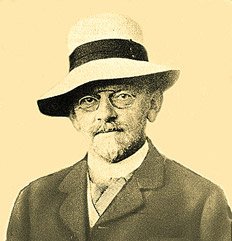
\includegraphics[scale=.4]{imagenes/Hilbert.jpg}\\
\end{center}
\small
<<David Hilbert (Königsberg, Prusia Oriental; 23 de enero de 1862-Gotinga, Alemania; 14 de febrero de 1943) fue un matemático alemán, reconocido como uno de los más influyentes del siglo XIX y principios del XX. Estableció su reputación como gran matemático y científico inventando y/o desarrollando un gran abanico de ideas, como la teoría de invariantes, la axiomatización de la geometría y la noción de espacio de Hilbert, uno de los fundamentos del análisis funcional. Hilbert y sus estudiantes proporcionaron partes significativas de la infraestructura matemática necesaria para la mecánica cuántica y la relatividad general. Fue uno de los fundadores de la teoría de la demostración, la lógica matemática y la distinción entre matemática y metamatemática. Adoptó y defendió vivamente la teoría de conjuntos y los números transfinitos de Cantor. Un ejemplo famoso de su liderazgo mundial en la matemática es su presentación en 1900 de un conjunto de problemas abiertos que incidió en el curso de gran parte de la investigación matemática del siglo XX.>> (Wikipedia)
}
\begin{quote}
 <<Nadie nos expulsará del paraíso que \index[personas]{Cantor} Cantor ha creado para nosotros>> 
\end{quote}
\begin{flushright}
 David Hilbert \index[personas]{Hilbert}
\end{flushright}






En esta unidad estudiaremos el concepto de
\index{Conjuntos!cardinal}\emph{cardinal} de un conjunto. Con este concepto se pretende dar
un significado a la noción de cantidad de elementos de un
conjunto, en especial cuando este es ``infinito''. Como se verá,
y por extraño que parezca, aunque el conjunto involucrado sea
infinito de todas maneras podremos definir el cardinal de ese
conjunto. Con esto implicitamente decimos que no todos los
conjuntos infinitos tendrán el mismo cardinal. Empezaremos
recordando algunas cuestiones básicas de teoría de
conjuntos que, a la vez, nos servirán como referencia para  las
notaciones.

%--------------------------------------------------------------
%SECCION




\section{Repaso nociones básicas sobre \index{Conjuntos} conjuntos}
La siguiente introducción está lejos de ser exhaustiva, solo
recordaremos conceptos ya sabidos. Nos dentendremos algo más en
aquellos puntos que puedan ser nuevos.

\begin{definicion}Dados dos conjuntos $A$ y $B$ denotaremos su \index{Conjuntos!union}\index{Conjuntos!intersección}\index{Conjuntos!diferencia}\emph{unión,
intersección y diferencia} por: $A\cup B$, $A\cap B$ y $A-B$
repectivamente. Estos nuevos conjuntos se definen por: \index[simbolos]{$A\cup B$}\index[simbolos]{$A\cap B$}\index[simbolos]{$A-B$}
\[A\cup B=\{x:x\in A\vee x\in B\},\]

\[A\cap B=\{x:x\in A\wedge x\in B\}\]
y

\[A-B=\{x:x\in A \wedge x\notin B\},\]
respectivamente.
\end{definicion}
 Por lo general, tendremos que los
conjuntos con los que trabajaremos estarán contenidos en un
conjunto que llamaremos el universo $\mathcal{U}$. Aceptado la
existencia de este universo, frecuentemente usaremos la siguiente
notación para el \emph{complemento} 
\[A^c=\mathcal{U}-A.\] 
\index[simbolos]{$A^c$}
Además consideraremos la operación de \index{Conjuntos!diferencia simétrica}\emph{diferencia simétrica},
definiéndose por:
\[A\bigtriangleup B=(A-B)\cup(B-A).\]
\index[simbolos]{$A\bigtriangleup B$}
\begin{definicion}Dados dos elementos arbitrarios $a$ y $b$ se
define el \emph{par ordenado}\index{par ordenado} $(a,b)$, por la siguiente igualdad
\[(a,b)=\{a,\{a,b\}\}.\]
\end{definicion}

La propiedad más relevante de pares ordenados es que si \index[simbolos]{$(a,b)$}
$(a,b)=(c,d)$ entonces $a=c$ y $b=d$. Eso se infiere de la demostración y queda como ejercicio. Ahora consideramos el
conjunto formado por todos los pares ordenados de elementos
pertenecientes a conjuntos dados.

\begin{definicion} Sean $A$ y $B$ conjuntos. El \index{Conjuntos!producto cartesiano}\emph{producto cartesiano} de $A$ con
$B$, denotado por $A\times B$, es el siguiente conjunto:
\[A\times B=\{(a,b):a\in A\wedge b\in B\}.\]
\end{definicion}
La siguiente definición es bien conocida.

\begin{definicion} Una \index{Función} \emph{función} $f$ de $A$ en $B$ (abreviaremos esta frase
porel siguiente símbolo: $f:A\longrightarrow B$)\index[simbolos]{$f:A\longrightarrow B$}, es un
subconjunto del producto cartesiano $A\times B$ con la propiedad
que: para todo $a\in A$ existe un único $b\in B$ tal que
$(a,b)\in f$. \end{definicion}

Suponemos que ya todos conocemos estos conceptos, asi como los
conceptos relacionados de: imagen, la notación $f(a)$, función
inyectiva, suryectiva y biyectiva. Admitimos todo esto por sabido.
Ahora introducimos una nueva notación.

\begin{definicion}
Por $B^A$ \index[simbolos]{$B^A$} denotamos al conjunto de todas las funciones
$f:A\longrightarrow B$.
\end{definicion}

Mas adelante daremos algunas explicaciones del porque de esta
notación.

Seguidamente damos las definiciones de los conjuntos imagen y preimagen de un conjunto dado por una función.

\marginnote{
\begin{center}
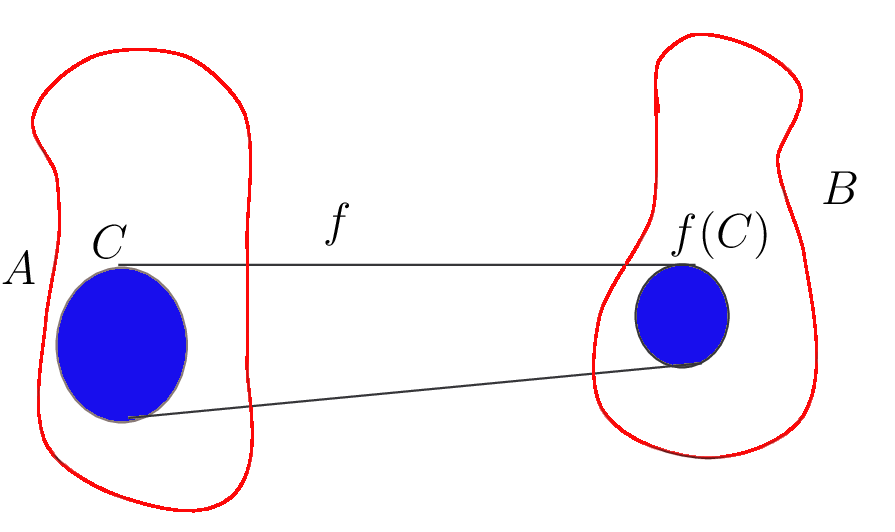
\includegraphics[scale=.15]{imagenes/funcima.png}\\
Conjunto $f(C)$
\end{center}
}
\begin{definicion} Dada una función $f:A\longrightarrow B$ y subconjuntos
$C\subset A$ y $D\subset B$ definimos:
\[f(C)=\{f(a):a\in C\}\]
y
\[f^{-1}(D)=\{a\in A:f(a)\in C\}.\]
\end{definicion}
\marginnote{
\begin{center}
 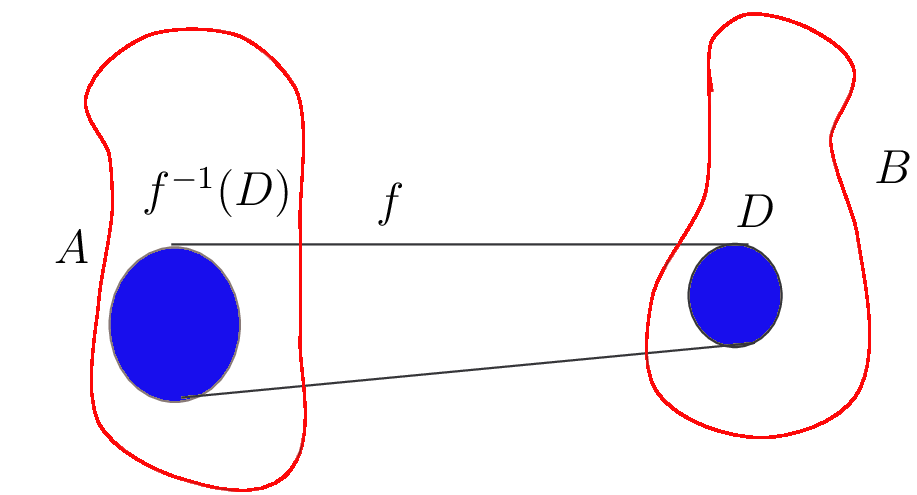
\includegraphics[scale=.15]{imagenes/fpreima.png}\\
 Conjunto $f^{-1}(D)$
\end{center}
}











Muy a menudo utilizaremos las propiedades que a continuación se
enuncian. Las demostraciones, de las mismas, quedaran a cargo del
alumno; ver Ejercicio \vref{3}.

\begin{proposicion}\label{propfunc} Sea $f:A\longrightarrow B$ una función.
Entonces
\begin{itemize}
\item[1.] $f(C_1\cup C_2)=f(C_1)\cup f(C_2).$
\item[2.]$f^{-1}(D_1\cup D_2)= f^{-1}(D_1)\cup f^{-1}(D_2).$
\item[3.] $f(C_1\cap C_2)\subset f(C_1)\cap f(C_2).$
\item[4.]$f^{-1}(D_1\cap D_2)= f^{-1}(D_1)\cap f^{-1}(D_2).$
\end{itemize}
\end{proposicion}


También vamos a considerar el \index{Conjuntos!partes}\emph{conjunto de partes} de un conjunto
dado, esto es el conjunto de todos sus subconjuntos.
Explícitamente:
\[\mathcal{P}(A)=\{C:C\subset A\}.\]
Se pueden efectuar uniones e intersecciones de una cantidad
arbitraria de conjuntos. Para poder enunciarlas debemos definir
antes lo que entendemos por una \emph{familia subindicada de
conjuntos} (o brevemente \emph{familia de conjuntos}).

\begin{definicion} Supongamos dado un conjunto $I$, al que nos referiremos como
conjunto de índices, y una función $i:I\longrightarrow
\mathcal{P}(A)$. Así tenemos que, para cada $i\in I$, existe
un único subconjunto de $A$, que llamaremos $A_i$. Diremos entonces que $\{A_i\}_{i\in I}$ es una familia
subindicada de conjuntos por el conjunto de índices $I$.
\end{definicion}

Ahora podemos definir la unión y la intersección de una
familia de esta índole de la siguiente manera
\begin{definicion} Definimos la unión e intersección de una
familia $\{A_i\}_{i\in I}$ por:
\[\bigcup_{i\in I}A_i=\{a:\exists i\in I:a\in A_i\}\]\index[simbolos]{$\bigcup_{i\in I}A_i$}
y
\[\bigcap_{i\in I}A_i=\{a:\forall i\in I:a\in A_i\}\]\index[simbolos]{$\bigcap_{i\in I}A_i$}
respectivamente.
\end{definicion}
En el Ejercicio \vref{propuniarb} podemos encontrar una serie de
propiedades de uniones e intersecciones de familias de conjuntos.
Estas propiedades las usaremos con frecuencia.
 Por último, en esta revisión de conjuntos, expondremos el
 axioma de elección. Este es un axioma de la teoría de
 conjuntos. Hay que aclarar que es posible axiomatizar la
 teoría de conjuntos, de esta axiomatización el mencionado axioma
 puede formar parte. Decimos ``puede'' por que este
 axioma ha despertado multitud de controversias en torno a su
 inserción o no en el restante conjunto de axiomas. No vamos a
 discutir aquí esta controversia ni tampoco la teoría
 axiomática de conjuntos pues esto nos desviaría de nuetros
 objetivos. Solo enunciaremos el \index{Axioma de elección}\emph{axioma de elección}, que
 usaremos frecuentemente.

\begin{axioma} Sea $\{A_i\}_{i\in I}$ una familia de conjuntos no
vacios. Entonces existe una función
\[f:I\longrightarrow\bigcup_{i\in I}A_i.\]
con la propiedad  que: 
\[\forall i\in I: f(i)\in A_i.\]
\end{axioma}



%--------------------------------------------------------------
%SECCION


\section{Definición de conjuntos coordinables}\marginnote{\vspace{-6cm}
\begin{center}
 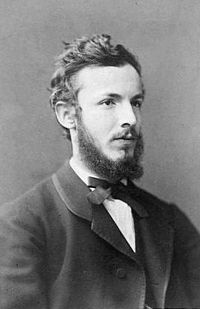
\includegraphics[scale=.4]{imagenes/Cantor.jpg}\\
 George Cantor (1845-1918)
\end{center}
\small
Georg Ferdinand Ludwig Philipp Cantor (San Petersburgo, 3 de marzo de 1845-Halle, 6 de enero de 1918) fue un matemático y lógico nacido en Rusia. Fue inventor con \index[personas]{Dedekind}\index[personas]{Frege}Dedekind y Frege de la teoría de conjuntos, que es la base de las matemáticas modernas. Gracias a sus atrevidas investigaciones sobre los conjuntos infinitos fue el primero capaz de formalizar la noción de infinito bajo la forma de los números transfinitos (cardinales y ordinales). 
(Wikipedia)}
En esta sección definimos el concepto clave de esta unidad, a
saber el concepto de que dos conjuntos sean \index{Conjuntos!coordinabilidad}\emph{coordinables}. Este concepto fue introducido y explotado por George Cantor.  Damos
una breve discución para motivar nuestra definición.

 Cuando
alguién cuenta algún conjunto de cosas, establece una
correspondencia entre los objetos que cuenta y un subconjunto de
números naturales. En el proceso de conteo,
algún objeto fue el primero en contarse, y se habrá dicho:
``uno'' para ese objeto. El proceso continua asignando,
sucesivamente, el número dos, tres, etc, a los restantes objetos
a contar, hasta que no queden más por contarse. Así, si en
este proceso llegamos hasta el 20, por ejemplo, decimos que hay 20
objetos. Aunque no haya que percatarse de eso a los fines
prácticos, lo que también hicimos fue establecer una
correspondencia o función entre los objetos y el conjunto
$\{1,\dots,20\}$. Más aún, esta correspondencia fue biyectiva
pues a cada número le correspondió solo uno de los objetos, es decir la función es inyectiva, y a cada objeto le
correspondió algún número, es decir  la función es
suryectiva. En otras palabras contar un conjunto significa
determinar el \index{intervalo inicial} \emph{intervalo inicial} del conjunto de los
números naturales para el cual exista una correspondencia biyectiva
con el conjunto que queremos contar. Conocer esto obviamente es
inútil a los efectos de contar cosas de la ``vida cotidiana'';
no obstante, es una observación fundamental a los efectos de
extender lo que llamamos ``contar'' a conjuntos infinitos. Lo que
antecede sugiere la siguiente definición.
\marginnote{ \emph{Intervalo inicial:}  un conjunto de
la forma: $\{j\in\mathbb{N}:1\leq j\leq n\}$, para cierto
$n\in\mathbb{N}$. De ahora en más, llamaremos a este conjunto:
$\mathbb{N}_n$}
\begin{definicion}\label{defcoordinables} Dados dos conjuntos: $A$ y $B$,
se dirá que ellos son coordinables, escribiremos \index[simbolos]{$A\thicksim B$}$A\thicksim B$,
si existe una función biyectiva $f:A\longrightarrow B$.
\end{definicion}

Esta es nuestra definición de que dos conjuntos, finitos o
no, tengan la misma cantidad de elementos. Como veremos, no
todos los  conjuntos infinitos son coordinables entre si. 
Es bueno notar que no es difícil demostrar que $\thicksim$ es
una relación de equivalencia (ver Ejercicio \vref{1}).
 Ahora
veamos algunos ejemplos.

\begin{ejemplo}Consideremos la función
$f:\nn\longrightarrow\{x\in\nn:x\,\,\text{es par}\}$, definida por
$f(x)=2x$. Facilmente se ve que $f$ es una biyección entre los
conjuntos indicados. De ahí que:
$\nn\thicksim\{x\in\nn:x\,\,\text{es par}\}$.
\end{ejemplo}

En este ejemplo observamos que, desde nuestro punto de vista, el
conjunto de los naturales tiene la misma cantidad de elementos
que el conjunto de los naturales pares. Es decir, según nuestra concepción de cantidad de elementos, el
todo no es mayor que una de sus partes. Este ejemplo ya lo había mencionado Galileo Galilei.

\begin{ejemplo}\label{rcoord(0,1)} Veamos que $\rr\thicksim (0,1)$. En este caso se
puede considerar la función

\[f(x):= \tan\biggl(\frac{2\pi x-\pi}{2}\biggr).\]
Dejamos como ejercicio corroborar que la función dada establece
una biyección entre los conjuntos involucrados.
\end{ejemplo}

Los dos ejemplos anteriores muestran una característica
importante de los conjuntos infinitos; un subconjunto de ellos
puede ser coordinable con el conjunto total. Mientras que, los
conjuntos finitos  carecen de esta característica.
Ver Ejercicio \vref{infcoordconsub}




%--------------------------------------------------------------
%SECCION

\section{Conjuntos numerables}
Hasta el momento hemos hablado de conjuntos
finitos e infinitos. Apelamos a la idea que todos nos forjamos en nuestras vidas  sobre el significado de estos términos .  Pero en este momento estamos  en condiciones, a
partir de la noción  de coordinalidad, de definir de forma
matemáticamente precisa los anteriores  significados.
\index{Conjuntos!finitos}\index{Conjuntos!infinitos}\index{Conjuntos!numerables}\index{Conjuntos!a lo sumo numerables}
\begin{definicion} Diremos que un conjunto $A$ es:
\begin{itemize}
\item[1.] \textbf{finito} si existe un $n\in\nn$ tal que
$A\thicksim\nn_n$.
\item[2.] \textbf{infinito }si no es finito.
\item[3.] \textbf{numerable} si $A\thicksim\nn$.
\item[4.] \textbf{a lo sumo numerable} si es finito o numerable.
\end{itemize}
\end{definicion}

En virtud de que $\thicksim$ es una realción de equivalencia, y
especialmente por el carácter transitivo de esta, si $A\thicksim
B$ y $B$ tiene alguna de las cuatro propiedades de la definición
anterior entonces $A$ tendrá esa misma propiedad.

Recordemos que, por definición, una sucesión $\{a_i\}$ de
elementos de un conjunto $A$ es una función
$f:\nn\longrightarrow A$, donde $a_i=f(i)$. Vemos así que el
concepto de numerabilidad está relacionado con el de sucesión.
En efecto, si el conjunto $A$ es numerable entonces sus elementos
se pueden disponer en una sucesión, donde ningún término se
repita.

Es oportuno que observemos que un conjunto no puede ser numerable
y finito a la vez; dicho de otra forma, los conjuntos numerables
son infinitos. Esto, como hemos definido los conceptos numerable y
finito de  manera precisa, tiene que ser demostrado.

\begin{teorema}\label{nesinfinito} Un conjunto numerable es
infinito.
\end{teorema}
\begin{demo} Supongamos que, por lo contrario, existe un conjunto
$A$ numerable y, a la vez, finito. Así tendríamos que:
$A\thicksim\nn$ y $A\thicksim\nn_n$, para algún $n\in\nn$. Como
$\thicksim$ es una relación de equivalencia , deducimos que
$\nn\thicksim\nn_n$. Sea, pues, $f$ una biyección:
$f:\nn_n\longrightarrow\nn$. Ahora consideremos el
natural\footnote{El símbolo $:=$ se lee \emph{igual por
definición}. Esto es, el miembro de la izquierda es definido por
el de la derecha}: $k:=f(1)+\dots+f(n)+1$. Como $f$ es una
biyección, existe algún $m$, con $1\leq m\leq n$ tal que
$f(m)=k$. Es decir
\[f(m)=f(1)+\dots+f(n)+1.\]
Seguramente, en el miembro derecho, uno de los términos es
$f(m)$. Este se puede cancelar con el miembro de la izquierda,
quedando
\[0=f(1)+\dots+f(m-1)+f(m+1)+\dots+f(n)+1.\]
Esta igualdad es absurda pues el miembro de la derecha es mayor
que $1$.
\end{demo}

Vamos a ver algunos otros conjuntos que también son numerables.
Empezamos por el siguiente.

\begin{proposicion}\label{subconjunto} Un subconjunto de un conjunto a lo sumo numerable es a
lo sumo numerable.
\end{proposicion}
\begin{demo} Sea $A\subset B$, con $B$ a lo sumo numerable. Se puede suponer
que $B\subset \nn$. ?`Por qué? Y, también podemos suponer que
$A$ es infinito, puesto que si fuera finito no habría nada
que probar. Definimos una función $f:\nn\longrightarrow A$ por
induccion. Puesto que los números naturales son bien ordenados,
tenemos que $A$ tiene un primer elemento, digamos, $a_1$.
Definamos
\[f(1)=a_1.\]
Ahora definimos $f(j)$ por:
\begin{equation}\label{frecursiva}
f(j)=\text{el primer elemento del conjunto: }A-\{f(i):1\leq i\leq
j-1\}. \end{equation} Esta definición es posible pues
$A-\{f(i):1\leq i\leq j-1\}\neq\emptyset$, de lo contrario $A$
sería finito. Queda así definida la función $f$. Resta
ver que es biyectiva.

Veamos, en primer lugar, que es inyectiva. Sea $i>j$. En virtud de
~\eqref{frecursiva}, tenemos que $f(i)\notin\{f(k):1\leq k\leq
i-1\}$ de lo cual, y como $j<i$, deducimos que $f(i)\neq f(j)$.

Ahora veamos la suryectividad. Supongamos que existe un elemento
$n\in A$ tal que $n\notin f(\nn)$. Recordemos la Definición
\eqref{frecursiva}. Ella nos dice, en virtud de que $n\notin
f(\nn)$, que $f(i)<n$, para todo $i$. Esto es debido a que $f(i)$
es el mínimo del conjunto $ A-\{f(k):1\leq k\leq i-1\}$ y a
que $n$ pertenece a ese conjunto. Tenemos, entonces, que
$f(\nn)\subset\nn_n$. Como consecuencia del Ejercicio \vref{1.5}
concluímos que $f(\nn)$ es finito. Pero como $f$ es inyectiva
$\nn\thicksim f(\nn)$. Lo que es una contradicción pues $\nn$ es
infinito.
\end{demo}

\begin{proposicion}\label{zesnum}
El conjuntos $\mathbb{Z}$, de los enteros,  es numerable.
\end{proposicion}
\begin{demo} Construímos una función que establece
una biyección entre los enteros positivos y los naturales pares
y entre los enteros negativos y los naturales impares. La
función es la siguiente:

\[f(x)=\left\{
\begin{array}{ll}
    2x+2, & \hbox{si $x\geq 0$;} \\
    -2x-1, & \hbox{si $x<0$.} \\
\end{array}
\right.\] Dejamos como ejercicio demostrar que, efectivamente, la
función $f$ es una biyección entre $\nn$ y $\mathbb{Z}$.
\end{demo}

\begin{proposicion}\label{NxNesnum} El conjunto $\nn\times\nn$ es numerable.
\end{proposicion}
\begin{demo} La demostración de este enunciado ya no es tan
sencilla. La idea se la debemos a G. Cantor. Primero presentaremos un razonamiento \href{https://es.wikipedia.org/wiki/Heur%C3%ADstica}{heurístico}  de
la construcción de la biyección entre $\nn\times\nn$
 y $\nn$. En rigor de verdad, a los efectos lógicos de la demostración, toda esta parte de la demostración
 se podría obviar; pudiéndose dar la fórmula
 ~\eqref{forfinal} sin dar ninguna justificación de como se nos
 ocurrió. Elegimos el camino contrario, explicar
 como obtener la fórmula.


 Dispongamos del conjunto $\nn\times\nn$ en un arreglo del tipo
de una ``matríz infinita'', como sigue:
\[\begin{diagram}
(1,1)   & \rTo        & (1,2)  &                      & (1,3)  &                      & (1,4) &\dots\\
        & \ldTo(2,2)  &        &\ldTo(2,2)\ruTo(4,2)  &        & \ldTo(2,2)\ruTo(6,4) &        &     \\
(2,1)   &             & (2,2)  &                      & (2,3)  &                      &        &      \\
        &\ldTo(2,2)   &        & \ldTo(2,2)           &        & \ddots               &        &      \\
(3,1)   &             &(3,2)   &                      &        &                      &        &      \\
        & \ldTo(2,2)  &        &   \ddots             &        &                      &        &      \\
 (4,1)  &             &        &                      &        &                      &        &      \\
 \vdots &             &        &                      &        &                      &        &      \\
\end{diagram}\]
Notar que, además de colocar los pares ordenados, hemos colocado
algunas flechas. Estas flechas indican un camino. Este es el
camino que seguiremos  para enumerar los pares ordenados.
Así, construiremos una función $f$ que hará las
siguientes asignaciones:

\begin{eqnarray}
    f:\nn\times\nn&\longrightarrow\nn\nonumber \\
    (1,1)&\longmapsto 1\nonumber \\
    (1,2)&\longmapsto 2\nonumber \\
     (2,1)&\longmapsto 3\nonumber\\
        &\hspace{-29pt}\vdots\nonumber \\
        \nonumber
\end{eqnarray}
Observar que en nuestro camino vamos siguiendo diagonales de
la matriz, de izquierda a derecha y de arriba hacia abajo. Cuando llegamos al margen izquierdo de la matriz
saltamos al borde superior, para luego descender por la
siguiente diagonal. Estas diagonales tienen $1, 2, 3, \dots$
elementos. Agrupemos los números naturales de esa forma, es
decir un primer grupo de uno, un segundo de dos y así
sucesivamente:

\[\underbrace{1}_{1} \underbrace{2\quad 3}_{2}\quad\underbrace{4\quad 5\quad
6}_{3}\quad \underbrace{7\quad 8\quad  9\quad 10}_{4}\dots
\]
Obsérvese que

\begin{equation}\label{numfinal}
\frac{j(j +1)}{2}=\text{número final del agrupamiento
$j$-ésimo}.
\end{equation}
Por ejemplo: el grupo cuarto tiene por su último elemento el 10,
que es igual a 4.5/2. Tambien tenemos que todos los pares
ordenados sobre la misma diagonal, tienen la característica
de que sus componentes suman lo mismo. Numeremos las diagonales,
de izquierda a derecha, empezando por 1. Así tenemos que la
diagonal 1 posee el elemento (1,1), la diagonal dos tiene los
elementos $(1,2)$ y $(2,1)$, etc. Por lo observado, tenemos la
siguiente fórmula, para cualquier par $(j,k)$

\begin{equation}\label{numdiag}
j+k-1=\text{el número de la diagonal a la que pertenece } (j,k).
\end{equation}
 El objetivo es poner en correspondencia la diagonal
$j$-ésima con el grupo $j$-ésimo de naturales. Notar que, en
virtud de ~\eqref{numfinal}, tenemos que
\begin{equation}\label{numdiag2}
\begin{split}\frac{(j+k-1)(j+k)}{2}=&\text{es el último número}\\
 & \text{del agrupamiento $j+k-1$-ésimo}.\\
\end{split}
\end{equation}
Así, si al primer miembro de ~\eqref{numdiag2} le restamos
$(j-1)$, obtenemos el número que ocupa el lugar $j$ (contando de
atras para adelante) del agrupamiento $j+k-1$ de naturales. Con
esto probamos que la función que queriamos construir es:


\begin{equation}\label{forfinal}
f(j,k):=\frac{(j+k-1)(j+k)}{2}-j+1.
\end{equation}
El resto de la demostración lo dejamos como ejercicio. Es decir la   demostración que ~\eqref{forfinal} es
biyectiva (ver Ejercicio \vref{2}).
\end{demo}

Como consecuencia del Ejercicio \vref{1.2} y de la Proposición
anterior, podemos afirmar que si $A$ y $B$ son numerables,
entonces $A\times B$ es numerable.



La siguiente propiedad también es útil para determinar si un
conjunto es numerable.

\begin{proposicion}\label{numinysur}Sean $A$ y $B$ conjuntos, con $B$ a lo sumo
numerable.
\begin{itemize}
\item[1.] Supongamos que existe una función inyectiva $f:A\longrightarrow
B$. Entonces $A$ es a lo sumo numerable.
\item[2.] Supongamos que existe una aplicación suryectiva
$f:B\longrightarrow A$. Entonces $A$ es a lo sumo numerable.
\end{itemize}
\end{proposicion}
\begin{demo} Veamos primero 1. La función $f$ es  una biyección entre $A$ y su
imagen $f(A)$. Como $B$ es a lo sumo numerable,  y como
consecuencia de la Proposición \vref{subconjunto}, tenemos que
$f(A)$ es a lo sumo numerable. Ahora, como $A\thicksim f(A)$
tenemos que $A$ es a lo sumo numerable.

Ahora probemos 2. Como $f$ es suryectiva, tenemos que $\forall
a\in A$: $f^{-1}(\{a\})\neq\emptyset$. Ahora, por el axioma de
elección sabemos que existe al menos una función
$g:A\longrightarrow B$ tal que $\forall a\in A:g(a)\in
f^{-1}(\{a\})$. Si pudiéramos probar que la función $g$ fuera
inyectiva, entonces obtendríamos la tesis a partir del inciso
1, que ya fue demostrado. Veamos, pues, que $g$ es inyectiva.
Supongamos que $a_1,a_2\in A$ y que $a_1\neq a_2$. Afirmamos que
$f^{-1}(\{a_1\})\cap f^{-1}(\{a_2\})=\emptyset$. En efecto, si
$b\in f^{-1}(\{a_1\})\cap f^{-1}(\{a_2\})$ entonces por un lado
 $f(b)=a_1$ y por otro $f(b)=a_2$, lo que es una contradicción pues $a_1\neq a_2$.
\end{demo}

Es interesante hacer notar que, utilizando el teorema anterior,
podemos dar otra demostración, más concisa, de la
Proposición \vref{NxNesnum}.

En esta demostración hacemos uso del Teorema Fundamental de la
Aritmética. Recordemos lo que este teorema nos dice:


\begin{teorema}[Fundamental de la Aritmética] Todo entero positivo $n$ se representa, de
manera única, de la forma $n=p_1^{\alpha_1}p_2^{\alpha_2}\dots
p_j^{\alpha_j}$, donde $p_1$, $p_2$,...,$p_j$ son números primos
y $\alpha_1$, $\alpha_2$,...,$\alpha_j$ son enteros positivos.
\end{teorema}

\begin{demo} \emph{alternativa de la Proposición \ref{NxNesnum}}
Definimos la siguiente función

\[\begin{split}
f:\nn\times\nn&\longrightarrow\nn\\
 (n,m)&\longrightarrow 2^n3^m\\
 \end{split}.
 \]
Por el Teorema Fundamental de la Aritmética, y mas precisamente
por la unicidad de la representación, tenemos, como $2$ y $3$
son primos, que si $2^n3^m=2^{n^{\prime}}3^{m^{\prime}}$ entonces
$n=n^{\prime}$ y $m=m^{\prime}$. Por consiguiente la función $f$
es inyectiva. Ahora, invocando la Proposición \vref{numinysur}
concluímos que $\nn\times\nn$ es a lo sumo numerable. Lo que
resta es, solo, ver que $\nn\times\nn$ no es finito. Esto se puede
probar observando que $\nn\times\nn$ contiene el subconjunto
$A=\{(1,n):n\in\nn\}$ que es coordinable con $\nn$, ?`Cuál es la
biyección?, y por consiguiente infinito. Así,
$\nn\times\nn$ no puede ser finito, si lo fuera, $A$ también lo
sería, por ser un subconjunto de él. Lo que concluye la
demostración.
\end{demo}

Ahora podemos demostrar  uno de los resultados más interesantes
de esta teoría.

\begin{teorema} El conjunto $\mathbb{Q}$ es numerable.
\end{teorema}
\begin{demo} Sabemos que $\mathbb{Z}$ es numerable y dejamos como ejercicio demostrar que $\mathbb{Z}-\{0\}$ es numerable. Consecuentemente también  $\mathbb{Z}\times\mathbb{Z}-\{0\}$ es numerable. Podemos
definir la siguiente función:
\[
\begin{split}
f:\mathbb{Z}\times\mathbb{Z}-\{0\}&\longrightarrow\mathbb{Q}\\
(n,m)&\longmapsto \frac{n}{m}
\end{split}
.\] Esta aplicación es suryectiva. Por consiguiente, usando la
parte 2. de la Proposición \vref{numinysur}, obtenemos que
$\mathbb{Q}$ es a lo sumo numerable. Así $\mathbb{Q}$ es
finito o numerable. Pero como $\mathbb{Q}$ es infinito, pues
$\nn\subset\mathbb{Q}$, tenemos que $\mathbb{Q}$ es numerable. \end{demo}


Traduciendo nuestra interpretación de que dos conjuntos
coordinables tienen la misma cantidad de elementos, vemos que hay
tantos racionales como naturales. Esta afirmación es un tanto
desconcertante. Sabemos que los racionales son
densos dentro de los reales. Esto quiere decir que dentro de cada
intervalo abierto, por chico que este fuere, siempre hay números
racionales dentro. Sin embargo, uno puede poner en correspondencia
$\nn$ y $\mathbb{Q}$.  

A esta altura pareciera que
todos los conjuntos resultan ser numerables, pero ya veremos, en
la sección siguiente, que no es así.


\begin{lema}\label{subconjnum} Todo conjunto infinito tiene un
subconjunto numerable.
\end{lema}

\begin{demo} Sea $A$ un conjunto infinito. Usaremos un argumento similar a la demostración de
la Proposición \vref{subconjunto}. Definimos inductivamente una
función $f:\nn\longrightarrow A$  de la siguiente manera. Puesto
que $A$ es infinito, en particular, es no vacio, así podemos
encontrar un elemento $a_1\in A$. Ponemos entonces
\[f(1)=a_1.\]
Ahora, supongamos que tenemos definida la función $f$, de tal
manera que sea inyectiva, para $j=1,\dots n$. Llamemos $f(j)=a_j$,
para $j=1,\dots , n$. Como $A$ es infinito no puede ocurrir que
$A-\{f(1),\dots,f(n)\}=\emptyset$, de lo contrario $f$ además de
ser inyectiva, de $\nn_n$ en $A$, sería suryectiva; y de este
modo $A\thicksim\nn_n$ lo que implica que $A$ es finito,
contrariando nuestra hipótesis. Por consiguiente, podemos
encontrar $a_{n+1}\in A-\{f(1),\dots,f(n)\}$. Definimos
$f(n+1)=a_{n+1}$.

Ahora veamos que $f$ así definida es inyectiva. Sea $i\neq
j $, podemos suponer que $i<j$. Sabemos que:
\[f(j)\notin \{f(1),\dots,f(j-1)\}.\]
Seguramente $f(i)$ es un elemento del conjunto de la derecha, en
la relación anterior, de modo que $f(j)\neq f(i)$, lo que
demuestra la inyectividad. Ahora, $f$ es biyectiva de $\nn$ en
$f(\nn)$. Por consiguiente $f(\nn)$ es un subconjunto de $A$
numerable. 
\end{demo}

La siguiente proposición es útil para probar que algunos
conjuntos son numerables. Antes de enunciarla, haremos una
observación útil a la demostración. Afirmamos que si $A$ es
un conjunto a lo sumo numerable, entonces existe una función
suryectiva de $\nn$ en $A$. En efecto, si $A$ es numerable, esto
es claro puesto que existe una biyección de $\nn$ en $A$. Si,
por el contrario, $A$ es finito, entonces existe una biyección
de $\nn_n$, para algún $n\in\nn$, en $A$; en este caso
extendemos la biyección a todo $\nn$ de cualquier
forma\footnote{Por ejemplo: ponemos $f(j)=1$ para $j>n$}, la
función resultante es suryectiva, aunque ya no inyectiva.

\begin{proposicion}\label{unionnumdenum} Sea $I$ un conjunto de índices a lo sumo
numerable. Supongamos que para cada $i\in I$ tenemos un conjunto
$A_i$ que, también, es a lo sumo numerable. Entonces
\[\bigcup_{i\in I}A_i\]
es a lo sumo numerable. Brevemente: ``Una unión a lo sumo
numerable de conjuntos a lo sumo numerables es a lo sumo
numerable''.
\end{proposicion}

\begin{demo} Como vimos, para cada $i\in I$ existe una función
suryectiva $f_i:\nn\longrightarrow A_i$. Definimos:
\[\begin{split}
      f:\nn\times I &\longrightarrow \bigcup_{i\in I}A_i\\
         (n,i)&\longmapsto f_i(n).\\
 \end{split}
\]
Esta función es suryectiva, pues si
\[a\in\bigcup_{i\in I}A_i,\]
entonces $a\in A_{i_0}$, para algún $i_0$; ahora, utilizando la
suryectividad de $f_{i_0}$, obtenemos un $n\in\nn$ tal que
$f_{i_0}(n)=a$. Es decir $f(n,i_0)=a$. Esto prueba que $f$  es
suryectiva. Ahora, como $\nn\times I$ es a lo sumo numerable, en
rigor es numerable, y por la Proposición \vref{numinysur},
obtenemos la tesis.
\end{demo}


\section{Un conjunto no numerable} \index{Conjuntos;no numerables}
Vimos que $\nn$ es numerable, por definición, y que $\mathbb{Z}$
y $\mathbb{Q}$ son también numerables. Ahora mostraremos un
conjunto que no es a lo sumo numerable. No será otro que el
conjunto de los numeros reales.


\begin{teorema}\label{realnonum} El conjunto $\mathbb{R}$ no es
a lo sumo numerable.
\end{teorema}
\begin{demo} Supongamos, por el contrario, que $\mathbb{R}$ es a
lo sumo numerable. En virtud de la Proposición
\vref{subconjunto}, tendríamos que el intervalo $[0,1)$
sería también a lo sumo numerable. Como él es infinito
entonces $[0,1)$ sería numerable. Sea, entonces, una
función biyectiva $f:\nn\longrightarrow [0,1)$. Definamos
$a_j:=f(j)$.

Como es sabido, cada número real $r$ admite un desarrollo en
expresión decimal infinita del tipo

\[r=0.r_1r_2r_3\dots.\]
Un peque\~no inconveniente lo presenta el hecho de que esta
expresión decimal no es única, puesto que, por ejemplo:
$2.000\dots=1.999\dots$. Para avolir este problema convenimos que
en nuestros desarrollos decimales no usaremos expresiones que
tienen todos $9$ a partir de cierto momento. Con esta
convención, el desarrollo decimal es único.

A los fines de clarificar nuestra demostración, es útil poner
a la sucesión $a_j$ de la siguiente manera :
\[\begin{split}
a_1&=0.a_{1,1}a_{1,2}a_{1,3}\dots\\
a_2&=0.a_{2,1}a_{2,2}a_{2,3}\dots\\
\vdots&\\
a_n&=0.a_{n,1}a_{n,2}a_{n,3}\dots\\
 \vdots&\\
 \end{split}\]
Ahora definimos un número $r=0.r_1r_2\dots\in[0,1)$, tomando en
cuenta los valores de $a_{i,j}$ sobre la digonal principal, que
por fuerza no será ninguno de los $a_j$. La definición es la
siguiente:
\[r_n:=\left\{
\begin{array}{ll}
    2, & \hbox{si $a_{n,n}<2$;} \\
    1, & \hbox{si $a_{n,n}\geq 2$.} \\
\end{array}
\right.
\]
Tenemos que $r\neq a_j$ para todo $j$, pues, estos números
seguramente son distintos en el lugar $j$ de su desarrollo.
Observar que si $a_j$ tiene un número menor que 2 en ese lugar,
entonces $r_j=2$, en cambio si un número mayor o igual que 2
ocupa el lugar $j$ de $a_j$, entonces $r_j=1$. Por ende, como
dijimos $r$ no es ningún $a_j$. Esto demuestra que la función
$f$ no es suryectiva.
\end{demo}

Utilizando el Ejemplo \vref{rcoord(0,1)} y el Ejercicio \vref{5},
vemos que $\rr\thicksim (0,1)\thicksim [0,1]$. Para cualquier
intérvalo no trivial\footnote{Por un intérvalo trivial
entendemos un intérvalo que se reduce a un punto} $I$,  ya sea
abierto o cerrado, existe una biyección, de hecho una función
lineal, de $I$ en el intérvalo $(0,1)$ o $[0,1]$, dependiendo de
si $I$ es cerrado o abierto. Vemos así que todos los
intérvalos no triviales son coordinables entre si y a su vez
con $\rr$.



\section{Una aplicación}
En esta sección daremos una aplicación de los conceptos
desarrollados en las secciones previas. Veremos como estos se
pueden usar para demostrar la existencia de números
trascendentes. Antes empezaremos con algunas definiciones.

Un polinomio es una expresión de la forma:
\[P(X)=a_0+a_1X+a_2X^2+\dots+a_nX^n,\]
donde $n\in\nn$ se llama \emph{grado} del polinomio y los $a_j$
\emph{coeficientes} del polinomio.  Escribiremos que $P\in
\mathbb{Z}[X]$, $P\in\mathbb{Q}[X]$ o $P\in\mathbb{C}[X]$ si los
coeficientes son enteros, racionales o complejos respectivamente.
Una raíz del polinomio $P$ es un número
$\alpha\in\mathbb{C}$ tal que
\[P(\alpha)=0.\]

Observar que un número racional $q=n/m$ es solución (o
raíz del polinomio) de la siguiente ecuación:
\[P(X):=mX-n=0.\]
Notar que este polinomio $P$ es de primer grado y además
$P\in\mathbb{Z}[X]$. Reciprocamente, si $q$ es solución de una
ecuación polinomial $P(X)=0$, donde $P$ es de primer grado y con
coeficientes en $\mathbb{Z}$, entonces $q$ es racional.

Hemos aprendido que hay dos clases de reales,\index{Números!racionales}\index{Números!irracionales} \emph{racionales e
irracionales}. En esta sección expondremos otros tipos de
números reales, a saber los \emph{trascendentes}\index{Números!trascendentes}. 


Tomemos por caso el
número $\sqrt{2}$, que como sabemos es irracional. A pesar de
ello $\sqrt{2}$ es solución de una ecuación a coeficientes
enteros de  segundo grado. Nos referimos a
siguiente:
\[X^2-2=0.\]
Vemos que $\sqrt{2}$ tiene, si se nos permite por el momento esta
expresión, un grado de irracionalidad no muy grande, puesto
que es solución de una ecuación de segundo grado a
coeficientes enteros. A estos números se los llama \index{Números!irracionales cuadráticos} \emph{irracionales cuadráticos}.

Nos preguntamos ahora si existiran números que acorde con la perspectiva anterior tengan el mayor grado
de irracionalidad  posible. Esto es que no sean solución de
ninguna ecuación polinomial a coeficientes enteros, no importa
del grado que fuere. Llamaremos a estos números, cuya existencia
es hipotética por el momento, \emph{trascendentes}. A los
restantes números los llamaremos \index{Números!algebraicos} \emph{algebraicos}. Denotaremos
por $\mathbb{A}$ al conjunto de números algebraicos y por
$\mathbb{T}$ al conjunto de números trascendentes. Cualquier
número que sea obtenido por medio de raices, del grado que
fuere, de números enteros son algebraicos. Esto indica que
resolver el problema planteado puede no ser fácil.

El problema de la existencia de números trascendentes fue
resuelto por \index[personas]{Liouville}Liouville en 1844. El demostró que el número
\[L=\sum_{n=0}^{\infty}\frac{1}{10^{n!}}\]
es trascendente. Posteriormente C. Hermite\index[personas]{Hermite} demostró en 1873
que $e=2.7172...$ es trascendente y Lindemann\index[personas]{Lindemann}, en 1882, que $\pi$
también lo es.

En esta sección mostraremos el argumento usado por G. Cantor, en
1874, para demostrar la existencia de números trascendentes. La
situación es la siguiente: Cantor demostró que el conjunto de
los números algebraicos es numerable. Luego, si el conjunto de
los trascendentes lo fuera, también lo sería el conjunto
$\rr$ (unión de dos numerables es numerable), lo cual no es
cierto. Asi es que no solo los números trascendentes existen,
sino que existen tantos como números reales hay. Dicho de otro
modo, los números trascendentes son los más comunes entre los
números reales. Los racionales, por el contrario, son una
excepción, habiendo de ellos solo una cantidad numerable.

Es bueno comentar que hubo matemáticos  que se opusieron a
G.Cantor y a su Teoría de Conjuntos. Quizas la gota que
rebalso el vaso fue la anterior demostración de la existencia
de números trascendentes. Pues es una manifestación de que la 
teoría de Cantor podía ser utilizada para demostrar cuestiones 
matemáticas profundas que no aparentaban tener nada que ver con
la teoría de conjuntos.

La clave de la demostración es el siguiente lema.

\begin{lema} El conjunto $\mathbb{Z}[X]$ es numerable.
\end{lema}
\begin{demo} Un polinomio  en $\mathbb{Z}[X]$ y de grado $n$ se puede
identificar con la $n+1$-upla de enteros formada por sus
coeficientes. Teniendo en cuenta esto, definimos la siguiente
función:
\[\begin{split}
          f:\mathbb{Z}[X]&\longrightarrow
            \bigcup_{n=1}^{\infty}\mathbb{Z}^n\\
            a_0+a_1X+\dots+a_nX^n&\longmapsto (a_0,a_1,\dots,
            a_n)\\
            \end{split},
\]
donde
\[\mathbb{Z}^n:=\underbrace{\mathbb{Z}\times\dots\times\mathbb{Z}}_{n\,\,\text{veces}}.\]
Por lo dicho con anterioridad, esta función es biyectiva.

Ahora bien, el conjunto $\mathbb{Z}^n$ es numerable. Podemos
probar esto usando inducción y el hecho de que el producto
cartesiano de conjuntos numerables es numerable. Así, como
consecuencia de la Proposición \vref{unionnumdenum} obtenemos
que
\[\bigcup_{n=1}^{\infty}\mathbb{Z}^n\]
es numerable. Como $f$ es una biyección, $\mathbb{Z}[X]$ es
numerable.
\end{demo}

Como corolario obtenemos que el conjunto de números algebraicos
es numerable.

\begin{corolario}\label{algsonnum}
El conjunto de números algebraicos es numerable.
\end{corolario}
\begin{demo} Se tiene que
\[\mathbb{A}=\bigcup_{P\in\mathbb{Z}[X]}\{\alpha:P(\alpha)=0\}.\]
Como es sabido de los cursos de álgebra, dado un polinomio $P$,
de grado $n$, el conjunto $\{\alpha:P(\alpha)=0\}$ es finito, es
mas, tiene a lo sumo $n$ elementos. Ahora, en virtud de esto y la
Proposición \vref{unionnumdenum}, obtenemos que $\mathbb{A}$ es
a lo sumo numerable. Ciertamente, este conjunto es infinito, pues
$\nn$ está contenido en él, de modo que no tiene mas chance
que la de ser numerable.
\end{demo}

Como otro corolario  obtenemos que
$\mathbb{T}\neq\emptyset$. Pues de lo contrario, como
$\rr=\mathbb{A}\cup\mathbb{T}$ y como la unión de a lo sumo
numerables es a lo sumo numerable, tendríamos que $\rr$
sería a lo sumo numerable, que es una contradicción. Pero
en realidad podemos demostrar algo más que
$\mathbb{T}\neq\emptyset$; podemos probar que
$\mathbb{T}\thicksim\rr$. Esto es consecuencia del siguiente
teorema, que afirma que al sacarle un conjunto numerable a un
conjunto coordinable con $\rr$ no alteramos la cantidad de
elementos del conjunto.
\begin{lema} Sean $A\thicksim\rr$ y $B\thicksim\nn$ tales que
$B\subset A$. Entonces $A-B\thicksim\rr$.
\end{lema}
\begin{demo} Tenemos que $A-B$ es infinito, de lo contrario, por la
Proposición \vref{unionnumdenum}, $A=(A-B)\cup B$ sería a
lo sumo numerable, contradiciendo nuestras hipótesis. Como $A-B$
es infinito, por el Lema \vref{subconjnum}, obtenemos un conjunto
numerable $C\subset A-B$. Como $B\cup C$ y $C$ son numerables,
existe una biyección $f:B\cup C\longrightarrow C$. Ahora
definimos la siguiente función:

\[
  \begin{split}
       \hat{f}:A&\longrightarrow A-B\\
       x\notin B\cup C&\longmapsto x\\
       x\in B\cup C&\longmapsto f(x)\\
  \end{split}.
\]
No es dificil demostar que $\hat{f}$ es una biyección, de donde
$A-B\thicksim A\thicksim\rr$.
\end{demo}

\begin{corolario} $\mathbb{T}\thicksim\rr$.
\end{corolario}
\begin{demo} Aplicando el lema anterior, con $A=\rr$ y
$B=\mathbb{A}$, obtenemos la tesis.
\end{demo}

\section{Comparación de cardinales}
En esta sección introduciremos una relación de orden entre
conjuntos, esta, intuitivamente, corresponderá a la noción de:
``tiene más elementos''. Para conjuntos
finitos todos estamos muy familiarizados con esta noción. También se suele decir que un conjuto
tiene un cardinal mayor que el otro, para expresar esta idea de
mayor cantidad de elementos. Informalmente ya hemos usado esta
noción al decir que había más números reales que
naturales. No obstante, en aquel momento, esa afirmación solo
constituyó una interpretación de cierto resultado, otra manera
de decirlo que fuera común a nuestra experiencia. En todo caso,
no fue ni una definición, ni un teorema, ni nada que fuera
plausible de ser demostrado. En esta sección,  formalizaremos el
concepto de y posteriormente analizaremos
algunas consecuencias de este.

Intuitivamente, decíamos que había más reales que
naturales por que $\nn\subset\rr$ y por que\footnote{Por $\nsim$
entendemos no coordinable} $\nn\nsim\rr$. Si queremos comparar dos
conjuntos cualesquiera, puede ocurrir que ninguno de ellos sea un
subconjunto del otro, o más aún que estos conjuntos sean
disjuntos. ?`Cómo procedemos en ese caso?. Veamos un ejemplo.
Consideremos el conjunto $\nn_0:=\nn\times
\{0\}=\{(n,0):n\in\nn\}$. ?`Cómo podríamos comparar este
conjunto con $\rr$?. Tenemos que $\nn_0\cap\rr=\emptyset$, sin
embargo, dentro de $\rr$ tenemos un subconjunto, precisamente
$\nn$, que es coordinable con $\nn_0$ a traves de la biyección
definida por $f(n,0)=n$. Podríamos decir entonces que, como
$\nn$ tiene menos elementos que $\rr$ y $\nn_0$ tiene la misma
cantidad que $\nn$, entonces $\nn_0$ tiene menos que $\rr$.
Notemos que la función $f$, que es biyectiva de $\nn_0$ en
$\nn$, es una aplicación inyectiva de $\nn_0$ en $\rr$.
Esperemos que la discución de este ejemplo muestre la
siguiente definición como natural.

\begin{definicion}\label{relorden} Dados dos conjuntos $A$ y $B$, diremos que
$A\precsim B$ si existe una aplicación inyectiva
$f:A\longrightarrow B$. Si, además, $A\nsim B$ diremos entonces
que $A\prec B$.
\end{definicion}


\begin{ejemplo} Si $A$ es un conjunto infinito, entonces
$\nn\precsim A $. Esto es consecuencia del Lema \vref{subconjnum}
\end{ejemplo}

\begin{ejemplo} Si $A$ es un conjunto finito entonces $A\prec\nn$.
Esto es consecuencia de la definición y del Teorema
\vref{nesinfinito}.
\end{ejemplo}

\begin{ejemplo} Tenemos las siguientes relaciones
\[\nn\thicksim\mathbb{Z}\thicksim\mathbb{Q}\thicksim\mathbb{A}\prec\mathbb{T}\thicksim\rr.\]
\end{ejemplo}

\begin{ejemplo} Si $A\prec B$, $A\thicksim C$ y
$B\thicksim D$, entonces $C\prec D$. A continuación justificamos esta afirmación. A causa de las
hipótesis, existen: una función inyectiva $f:A\longrightarrow
B$ y funciones biyectivas: $g:C\longrightarrow A$ y
$h:B\longrightarrow D$.
\[
    \begin{diagram}
      A         & \rTo^{f}                  & B\\
       \uTo^{g} &                            &\dTo^{h}\\
       C        &\rTo^{h\circ f\circ g}                    &D\\
       \end{diagram}
       \]
La función $h\circ f \circ g$ es inyectiva, lo que demuestra que
$C\precsim D$. Deberíamos ver que $C\nsim D$. Supongamos que,
por el contrario, $C\thicksim D$. Sea $\phi:C\longrightarrow D$
una biyección entonces tendríamos el siguiente diagrama
\[
    \begin{diagram}
      A             &\rTo^{h^{-1}\circ\phi\circ g^{-1}}     & B\\
      \dTo^{g^{-1}} &                                       & \uTo^{h^{-1}}\\
      C              &\rTo^{\phi}                            &D\\
       \end{diagram}
       \]
y, puesto que las funciones intervinientes son todas biyecciones,
tendríamos que $A\thicksim B$, contradiciendo, esto, nuestras
hipótesis.
\end{ejemplo}

En el siguiente teorema podemos ver que para cualquier conjunto
$A$ hay otro conjunto que es mas grande, en el sentido de la
Definición \vref{relorden}. Este conjunto será el conjunto de
partes $\mathcal{P}(A)$.

\begin{teorema}[Cantor]\label{teorcantor} Para todo conjunto $A$, $A\prec\mathcal{P}(A)$.
\end{teorema}
\begin{demo} Tenemos que probar que: $A\precsim\mathcal{P}(A)$ y
$A\nsim\mathcal{P}(A)$. La siguiente función:

\[\begin{split}
        f:A&\longrightarrow\mathcal{P}(A)\\
          a&\longmapsto \{a\}
  \end{split}
\]
es inyectiva, de modo que $A\precsim\mathcal{P}(A)$.

Supongamos que existe una biyección
$g:A\longrightarrow\mathcal{P}(A)$. Definimos el subconjunto $B$
de $A$ de la siguiente manera
\[B:=\{a\in A:a\notin g(a)\}.\]
Como $g$ es suryectiva, existe un $b\in A$ tal que $g(b)=B$.
?`Será o no cierto que $b\in B$? Si es cierto, por definición
de $B$, tendríamos que $b\notin g(b)=B$, lo que es una
contradicción. Si fuera falso, es decir $b\notin B$, nuevamente
por la definición de $B$, deducimos que $b\in g(b)=B$, otra
contradicción. De modo que, no importando cual, todos los casos
nos conducen a una contradicción que es  fruto de suponer que
$A\thicksim\mathcal{P}(A)$.
\end{demo}

Una propiedad importante de $\precsim$ es su atisimetría,
esta propiedad no es facil de probar.

\begin{teorema}[Schr\"oder-Bernstein]\label{scho-ber} Si
$A\precsim B$ y $B\precsim A$ entonces $A\thicksim B$.
\end{teorema}

\noindent\emph{Idea de la demostración} Como dijimos, la
demostración de este teorema  no es tan sencilla. En primer
lugar, trataremos de explicar la idea que subyace en ella,  y
posteriormente la expondremos acabadamente.

Por las hipótesis, existen funciones inyectivas
$f:A\longrightarrow B$ y $g:B\longrightarrow A$. Si alguna de
estas funciones fuera suryectiva, entonces el teorema ya
estaría probado. De modo que podemos suponer que no son
suryectivas. Notar que $g:B\longrightarrow g(B)$ es una función
biyectiva.  Existe por lo tanto una
función inversa, que es biyectiva, $g^{-1}:g(B)\longrightarrow
B$ . Construiremos una biyección de $\tilde{f}:A\longrightarrow
B$, con el auxilio de $f$ y $g^{-1}$, de la siguiente manera:
Buscamos un subconjunto $\tilde{A}\subset A$ de forma tal que la
función:
\begin{equation}\label{ftilde}
\tilde{f}(a):=\left\{%
\begin{array}{ll}
    f(a), & \hbox{si $a\in \tilde{A}$;} \\
    g^{-1}(a), & \hbox{si $a\notin\tilde{A}$.} \\
\end{array}%
\right.
\end{equation}
sea biyectiva. Un primer requerimiento para esta función es que
$\tilde{A}^c\subset g(B)$. Esto a causa de que si
$a\in\tilde{A}^c$ entonces le aplicaremos $g^{-1}$ a ese $a$, por
consiguiente $a$ debería estar en el dominio de $g^{-1}$, que
es $g(B)$. Dicho de otro modo, se debe cumplir que
$g(B)^c\subset\tilde{A}$. Por simplicidad pongamos $A_1:=g(B)^c$ y
$B_1:=f(A_1)$. Ver la Figura \vref{figura3}


\begin{figure}[h]


\begin{center}
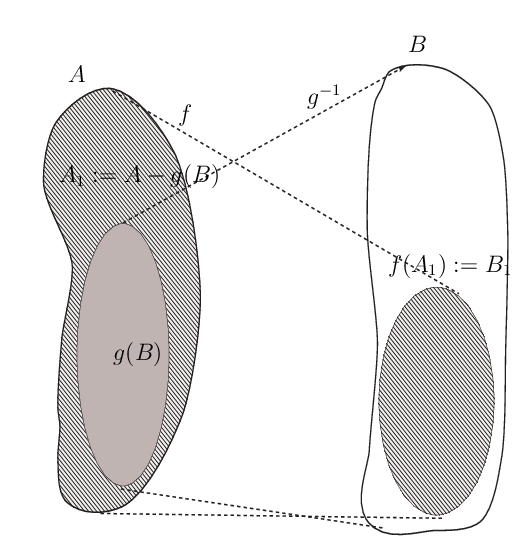
\includegraphics[scale=.5]{imagenes/supfyg.png}
\end{center}

 \caption{Las funciones $f$ y $g^{-1}$}\label{figura3}
\end{figure}

Una primera aproximación sería intentar la construcción
con $\tilde{A}=g(B)^c$. Seguramente así la función
$\tilde{f}$, ver ~\eqref{ftilde}, está bien definida. La
función $\tilde{f}$ será suryectiva, pues $g^{-1}$ es
suryectiva de $g(B)$ en $B$. No obstante, con esa elección de
$\tilde{A}$, la función $\tilde{f}$ no es inyectiva pues cada
elemento de $B_1$ es imágen, por esta $\tilde{f}$, de dos
elementos, uno en $A_1$ y otro en $g(B)$. De modo que esta
elección de $\tilde{A}$ todavía no nos sirve. Lo que vamos
a hacer ahora es agregarle a $\tilde{A}$ el conjunto de todos los
elementos de $g(B)$ tales que $g^{-1}$ los lleva a $B_1$. Este
conjunto es $A_2:=g(B_1)$. Definamos además $B_2:=f(A_2)$. Ahora
$\tilde{f}$ llevará $A_1\cup A_2$ en $B_1\cup B_2$. Nos
preguntamos, ahora, si la elección $\tilde{A}:=A_1\cup A_2$ nos
servirá. Lamentablemente, la respuesta es
no\footnote{Podría ser que si, si la función $f$ hubiera
sido biyectiva desde un principio, cosa que descartamos}. Al haber
agrandado $\tilde{A}$ también se nos agrandó el conjunto
de puntos en $B$ que son imagen de dos puntos, antes era el $B_1$,
ahora apareció el $B_2$. De modo que continuamos el proceso,
es decir, definimos $A_3:=g(B_2)$, $B_3:=f(A_3)$ y así
sucesivamente, ver Figura \vref{figura4} . Nunca llegaremos, en
una cantidad finita de pasos, al conjunto $\tilde{A}$ con la
propiedad deseada, puesto que al cabo de $n$ pasos se nos genera
el conjunto $B_n$ donde las imagenes continuan superponiendosé.
?`Qué haremos entonces?. Lo que se hará es seguir este proceso
indefinidamente, generando una sucesión de conjuntos $A_n$ y
$B_n$, y luego definir:

\begin{equation}\label{defatilde}
\tilde{A}:=\bigcup_{n=1}^{\infty}A_n.
\end{equation}


\index[personas]{Schr\"oder}\index[personas]{Berstein}
\begin{figure}[h]
 \begin{center}
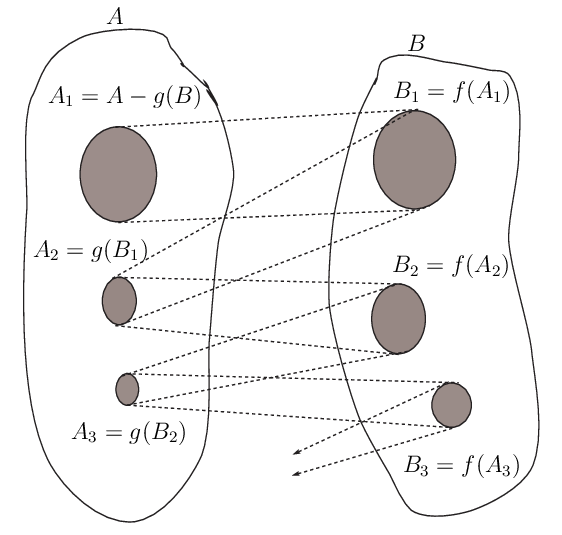
\includegraphics[scale=.5]{imagenes/schber4.png}
\end{center}
 \caption{Demostración del teorema de Schr\"oder-Berstein}\label{figura4}
\end{figure}

Intuitivamente, este conjunto debería  funcionar, es decir no
hay más superposición de $f$ con $g^{-1}$. Esto es pues si
$a\in\tilde{A}$ entonces $a\in A_n$, para algún $n$, y $f(a)\in
B_n$; eventualmente $f(a)$ podría ser igual a algún
$g^{-1}(a')$, pero $a'$ tendría que estar en $A_{n+1}$ y por
consiguiente está en $\tilde{A}$. Y así
$\tilde{f}(a')=f(a')$, y no $\tilde{f}(a')=g^{-1}(a')$, evitando
la superposición de imagenes.

\vspace{10pt}
\begin{demo}\emph{Teorema \ref{scho-ber}} Estamos en condiciones de hacer la demostración propiamente
dicha del teorema. Hasta ahora solo tratamos de explicar la
demostración. Definimos inductivamente conjuntos $A_n$ y $B_n$
de la siguiente manera:

\[\left\{%
\begin{array}{ll}
    A_1=g(B)^c, & B_1=f(A_1) \\
    A_{n+1}=g(B_n), & B_{n+1}=f(A_{n+1}) \\
\end{array}%
\right..\]

Definamos $\tilde{A}$  como en ~\eqref{defatilde} y $\tilde{f}$
como en ~\eqref{ftilde}. Veamos que $\tilde{f}:A\longrightarrow B$
es biyectiva, empezando por la inyectividad.

Sean $a,a'\in A$ dos puntos cualesquiera tales que
$\tilde{f}(a)=\tilde{f}(a')$. Si $a$ y $a'$ están
simultaneamente en $\tilde{A}$, o en $\tilde{A}^c$, tenemos que
$a=a'$ como consecuencia de que $f$ y $g^{-1}$ son inyectivas.
Consideremos entonces el caso $a\in\tilde{A}$ y $a'\notin
\tilde{A}$. Debemos llegar a una contradicción pues estamos
suponiendo indirectamente que $a\neq a'$, por estar en conjuntos
disjuntos, y que $\tilde{f}(a)=\tilde{f}(a')$. Tenemos que, para
algún $n\in\nn$, $a\in A_n$. Además, por la definición de
$\tilde{f}$,  $f(a)=g^{-1}(a')$. Por consiguiente
$g(f(a))=a'$. Como $a\in A_n$, $f(a)\in B_n$ y $a'=g(f(a))\in
A_{n+1}$. Esto contradice que $a'\notin\tilde{A}$.

Veamos ahora la suryectividad. Sea $b\in B$ cualquier punto. Si
$b\in B_n$, para algún $n$, como $B_n=f(A_n)$, ciertamente
existe un elemento $a\in A_n$ tal que $f(a)=b$. Ahora, por la
definición de $\tilde{f}$, $\tilde{f}(a)=f(a)=b$. Supongamos,
pues, que $b$ no está en ningún $B_n$. Como una afirmación
intermedia, probaremos que $g(b)$ no está en ningún $A_n$.
Supongamos, por el contrario, que existe un $n$ tal que $g(b)\in
A_n$. Tiene que ser $n>1$, pues $A_1=g(B)^c$ y $g(b)\in g(B)$.
Así, por su definición  y como $n>1$, el conjunto $A_n$ es
igual a $g(B_{n-1})$. De modo que $g(b)\in g(B_{n-1})$. Esto
implica que existe un $b'\in B_{n-1}$ tal que $g(b)=g(b')$. Pero,
como $g$ es inyectiva $b=b'$ y, por ende, $b\in B_{n-1}$.
Contradiciendo esto que $b$ no estaba en ningún $B_n$. Probamos,
así, que $g(b)$ no está en ningún $A_n$. Por lo tanto
$\tilde{f}(g(b))=g^{-1}(g(b))=b$. Vale decir $b=\tilde{f}(a)$ con
$a=g(b)$. Que era lo que queríamos probar.
\end{demo}

\section{Números Cardinales}
\marginnote{\vspace{-4cm}
\begin{center}
 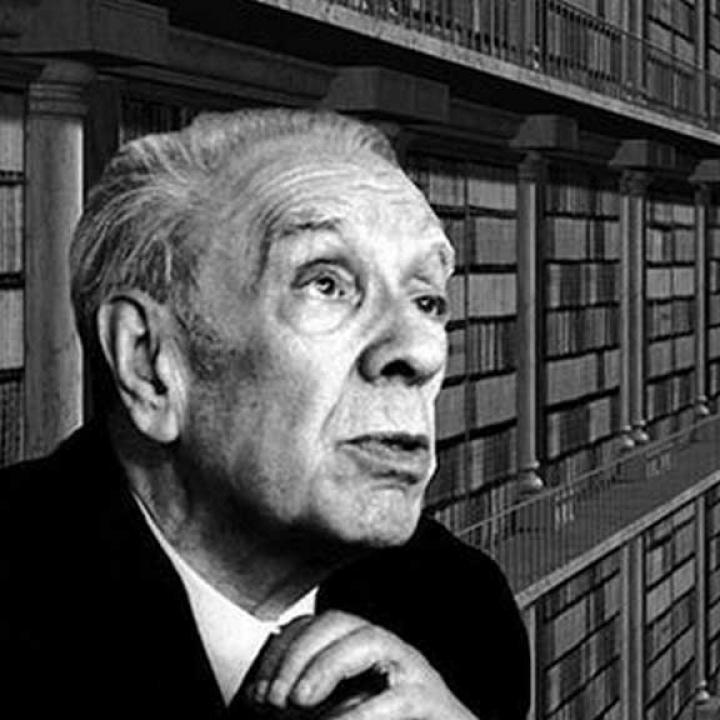
\includegraphics[scale=.13]{imagenes/Borges.jpg}\\
\end{center}
\small
<<Borges y la matemática es un libro de ensayo de 2006 de Guillermo Martínez que relata como varias ideas en la matemática moderna se hallan en la obra literaria del autor argentino Jorge Luis Borges, incluyendo conceptos como la teoría de conjuntos, recursión, la teoría de caos, y sucesión matemática infinita,1​ aunque los enlaces más fuertes que Borges tuvo con la matemática son a través de la teoría de conjuntos infinitos de Georg Cantor. El título del cuento El Aleph se alude al uso de la letra hebrea de Cantor, álef ( $\aleph$ ) por denotar cardinalidad de conjuntos transfinitos>> (Wikipedia)
}

Hasta el momento hemos introducido la noción de cuando dos conjuntos tienen la misma catidad de elementos. Pero no hemos definido el concepto de cantidad de elementos de un conjunto digamos $A$.  A grandes rasgos esto debería ser una característica de todos los conjuntos coordinables con $A$ y se denominará \index{Cardinal}\emph{cardinal} del conjunto $A$ y lo denotaremos por $\#A$. George Cantor defininió este concepto. La definición precisa demanda desarrollar la Teoría de números ordinales, que no es la intención de estas notas. Permítasenos pues invocar el concepto de cardinal a partir de la definición matemáticamente no satisfactoria que dimos, pero creemos que es bastante clara al entendimiento. 

 Se sabe que los números cardinales están ordenados bajo el orden es el definido en la sección anterior.  Concretamente escribiremos   $\#A< \#B$ cuando $A\prec B$. Se puede demostrar que este un buen orden, en el sentido que todo conjunto acotado inferiormente tiene primer elemento. 
 
 Desde George Cantor es costumbre denotar los números cardinales con letras del alfabeto hebreo. Así el primer \emph{cardinal transfinito}\index{Cadinal!transfinito}\footnote{Como es usual adoptaremos la denominación de transfinito en lugar de infinito como usamos hasta aquí} es el que le corresponde a los números naturales y se denota por $\aleph_0$.
 \index[simbolos]{$\aleph_0$} Como el conjunto de cardinales es bien ordenado existe un sucesor de $\aleph_0$ al que denominamos naturalmente $\aleph_1$. Al cardinal que corresponde a los números reales lo denominamos $c$. Sabemos que $\aleph_0<\aleph_1\leq c$ y George Cantor  conjeturó
que $c=\aleph_1$. Esta fue una de las más famosas conjeturas de la matemática y se denominó \href{https://es.wikipedia.org/wiki/Hipótesis_del_continuo}{La Hipótesis del Continuo}. George Cantor fracasó en hallar una demostración de la hipótesis del continuo.   El gran maremático Kurt G\"odel probó en 1938 que esta hipótesis es consistente con el sistema axiomático de la Teoría de conjuntos de  \index[personas]{Zermelo}\index[personas]{Fraenkel} Zermelo y Fraenkel, y por tanto puede ser tomado como un axioma nuevo para la teoría de conjuntos. Sin embargo, en 1963 \index[personas]{Cohen} Paul Cohen probó que la negación de la hipótesis del continuo también es consistente con los axiomas ZF, lo cual prueba que dicha hipótesis es totalmente independiente de los axiomas ZF. Esta situación es similar a la de las geometrías no euclídeas. 
\marginnote{\vspace{-2cm}
\begin{center}
 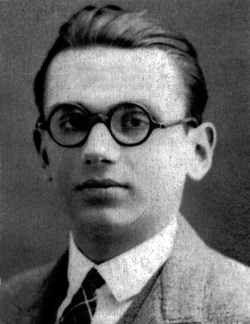
\includegraphics[scale=.3]{imagenes/godel.png}\\
\end{center}
\small
<<Kurt Gödel; Brünn, Imperio austrohúngaro, actual República Checa, 28 de abril de 1906-Princeton, Estados Unidos; 14 de enero de 1978) fue un lógico, matemático y filósofo austríaco.
\newline
Se le considera uno de los lógicos más importantes de todos los tiempos. Su trabajo ha tenido un impacto inmenso en el pensamiento científico y filosófico del siglo XX.  Gödel intentó emplear la lógica y la teoría de conjuntos para comprender los fundamentos de la matemática.
\newline
Se le conoce sobre todo por sus dos teoremas de la incompletitud, publicados en 1931. El más célebre establece que para todo sistema axiomático recursivo auto-consistente lo suficientemente poderoso como para describir la aritmética de los números naturales (la aritmética de Peano), existen proposiciones verdaderas sobre los naturales que no pueden demostrarse a partir de los axiomas. Para demostrar este teorema, desarrolló una técnica denominada ahora numeración de Gödel, que codifica expresiones formales como números naturales.\newline
También demostró que la hipótesis del continuo no puede refutarse desde los axiomas aceptados de la teoría de conjuntos, si dichos axiomas son consistentes. >> (Wikipedia)
}


No contento con introducir los números cardinales transfinitos George Cantor introdujo una aritmética entre ellos. Así por ejemplo si $\aleph_a$ y $\aleph_b$ son dos cardinales, buscamos dos conjuntos disjuntos cualesquiera $A$ y $B$ tales que $\#A=\aleph_a$ y $\#B=\aleph_b$ y definimos
\[
 \begin{split}
  \aleph_a+\aleph_b&=\#A\cup B\\
\aleph_a\times\aleph_b&=\#A\times B\\
\aleph_a^{\aleph_b}&=\#A^B\\
2^{\aleph_a}&=\#2^A
 \end{split}
\]
Algunas relaciones que hemos demostrado
\[
 \begin{array}{ccl}
  \forall \aleph: 2^\aleph &< \aleph & \text{(Por Teorema \ref{teorcantor})}\\  
   \aleph_0\times\aleph_0&=\aleph_0 &\text{(Por Proposición \ref{NxNesnum})}\\
   \aleph_0+\aleph_0&=\aleph_0 &\text{(Por Proposición \ref{unionnumdenum})}\\
   
 \end{array}
\]



\section{Aplicaciones del Teorema de Schr\"oder-Berstein}

El teorema de Schr\"oder-Berstein es una herramienta potente para
probar coordinabilidad de conjuntos puesto que nos permite establecer coordinabilidad mostrando sólo que existen funciones inyectivas entre los conjuntos.

Habíamos visto
que $\rr\nsim\nn$. ?` Qué ocurre con $\rr^2$, $\rr^3$,...?
?`Serán estos conjuntos más ``numerosos'' que $\rr$? Esto es:
?`Serán no coordinables con $\rr$?. Recordando que $\#\rr=c$ nos preguntamos si $c<c^2$. La respuesta a esta
pregunta es negativa, es decir $\rr^n\thicksim\rr$ esto es$c^n=c$. Para ver esto
basta demostrar que $(0,1)^2\thicksim (0,1)$. El caso general es
consecuencia del caso $n=2$, usando inducción, el Ejemplo
\vref{rcoord(0,1)} y el Ejercicio \vref{1.2}.

\begin{teorema} $(0,1)^2\thicksim (0,1)$. En otras palabras $c^2=c$. 
\end{teorema}
\begin{demo} Observar que $(0,1)\precsim (0,1)^2$. Para
demostrarlo considerar la función inyectiva $f(x)=(x,1/2)$.

Veamos que $(0,1)^2\precsim (0,1)$. Debemos construir una
función inyectiva $f:(0,1)^2\longrightarrow (0,1)$. Sea
$(x,y)\in (0,1)^2$. Consideremos las expresiones decimales
$x=0.x_1x_2...$ e $y=0.y_1y_2...$, donde $x_i$ e $y_i$ son enteros
entre 0 y 9, y no son todos 9 a partir de un momento en adelante.
Entonces escribimos:
\[f(x,y):=0.x_1y_1x_2y_2....\]
Es decir $f$ intercala las expresiones decimales de $x$ e $y$.
Esta función es inyectiva, puesto que dos expresiones decimales
iguales tienen todos sus dígitos correspondientes iguales.
Esto concluye la demostración.
\end{demo}

Es bueno notar que la función $f$, definida en la demostración
anterior, no es suryectiva. Un número que no es imagen de
ningún par es $0.909090...$. ?`Por qué será esto?

Por el Teorema \vref{teorcantor} tenemos que
$\nn\prec\mathcal{P}(\nn)$. Desmostramos, además, que $\nn\prec
\rr$. Nos preguntamos, ahora, que relación unirá
$\mathcal{P}(\nn)$ con $\rr$. Con el siguiente teorema probaremos
que aquellos conjuntos son coordinables.

\begin{teorema} $\mathcal{P}(\nn)\thicksim\rr$. En otras palabras $2^{\aleph_0}=c$.
\end{teorema}
\begin{demo} Probaremos que $\mathcal{P}(\nn)\precsim\rr$ y después que
$\mathcal{P}(\nn)\succsim\rr$.

 Como $\mathcal{P}(\nn)\thicksim\mathbf{2}^{\nn}$ ( Ejercicio \vref{6}), y por el
 Ejercicio \vref{1.2} inciso 4, probaremos que $\mathcal{P}(\nn)\precsim\rr$ si podemos
 probar que $\mathbf{2}^{\nn}\precsim \rr$. Para este fin,
 consideremos la siguiente función:
 \[
    \begin{split}
          T:\mathbf{2}^{\nn}&\longrightarrow \rr\\
           f&\longmapsto 0.f(1)f(2)f(3)...\\
    \end{split}
 .\]
Esto es la función $f$ se aplica en un número cuya expansión
decimal tiene solo ceros y unos. Esta función es inyectiva, pues
si
\[0.f(1)f(2)f(3)...=0.g(1)g(2)g(3)...\]
Entonces, por la unicidad de la expansión
decimal\footnote{Recordemos que puede haber expresiones decimales
distintas que representan el mismo número, estas son las
expresiones que tienen todos nueves a partir de un momento en
adelante, como por ejemplo 1=0.999....No obstante este problema no
se nos presenta aquí pues la expresiones decimales que
consideramos tienen solo 0 y 1}, tenemos que $f(1)=g (1)$,
$f(2)=g(2)$,.... Por consiguiente las funciones son iguales. Lo
que prueba la inyectividad. De este modo demostramos que
$\mathbf{2}^{\nn}\precsim \rr$ y esto, por lo que explicamos
anteriormente, implica que $\mathcal{P}(\nn)\precsim \rr$

Ahora debemos ver que $\mathcal{P}(\nn)\succsim\rr$. Utilizando
los  incisos 1. y 4. del Ejercicios \vref{1.2}, vemos que es
suficiente probar que $\rr\precsim \mathcal{P}(\mathbb{Q})$. Para
hacer esto definimos la siguiente aplicación:
\[
   \begin{split}
        T:\rr &\longrightarrow \mathcal{P}(\mathbb{Q})\\
        r &\longmapsto \{q\in\mathbb{Q}:q<r\}
   \end{split}
.\]

Veamos que  la aplicación es inyectiva. Sean $r_1,r_2\in\rr$
números reales distintos, supongamos $r_1<r_2$. Por la densidad
de $\mathbb{Q}$, existe un $q_0\in\mathbb{Q}$ tal que
$q_0\in(r_1,r_2)$. Así $q_0\in\{q\in\mathbb{Q}:q<r_2\}$ y
$q_0\notin\{q\in\mathbb{Q}:q<r_1\}$. De modo que
\[\{q\in\mathbb{Q}:q<r_1\}\neq\{q\in\mathbb{Q}:q<r_2\}.\]
Es decir $T$ es inyectiva.
\end{demo}
Para finalizar demostraremos que
$\nn^{\nn}\thicksim\mathbf{2}^{\nn}$. Mas que el resultado en
sí, vamos a resaltar su demostración, pues contiene una
idea interesante.

\begin{proposicion} $\nn^{\nn}\thicksim\mathbf{2}^{\nn}$. En lenguaje de cardinales  $\aleph_0^{\aleph_0}=2^{\aleph_0}$.
\end{proposicion}

\begin{demo} Dado un conjunto $X$ cualquiera, podemos interpretar una
función $f\in X^{\nn}$ como una sucesión de elementos de $X$,
a la que podemos disponer de la siguiente manera:
\begin{equation}\label{mensajes}
     f=(f(1),f(2),f(3),...).
\end{equation}
Si $X=\nn$ entonces la sucesión será de números naturales y
si $X=\mathbf{2}$ entonces la sucesión será de ceros y unos.

Interpretemos el segundo miembro de ~\eqref{mensajes}  como una
palabra infinita. Si $X=\nn$, esta palabras se compone de
``letras'' que pueden ser cualquier número natural. Si
$X=\mathbf{2}$, esta ``palabra'' se escribe con solo dos
``letras'' el 0 y el 1. La pregunta es: ?`Cómo podemos
``traducir'' una palabra escrita con un alfabeto de infitas
letras, a uno con solo dos?. La solución a esto es ingeniosa.
Sea $f\in\nn^{\nn}$, usaremos el signo 1 para denotar las comas en
la sucesión $f$ y pondrémos tantos ceros como indiquen las
cantidades $f(j)$.


\[
  \begin{split}
         T\quad:\quad\nn^{\nn}\quad\quad &\longrightarrow\quad\quad\mathbf{2}^{\nn}\\
         f=(f(1),f(2),f(3),...)&\longmapsto
          (\underbrace{0,...,0}_{f(1)\,\,\text{ceros}},1,
          \underbrace{0,...,0}_{f(2)\,\,\text{ceros}},1,....)\\
 \end{split}
\]
Veamos que esta función es inyectiva. Sean $f,g\in\nn^{\nn}$,
con  $f\neq g$. Sea
\[j=\min\{i:f(i)\neq g(i)\}.\]
Tenemos que $f(i)=g(i)$ para $i<j$. Escribamos las dos sucesiones

\[   (\underbrace{0,...,0}_{f(1)\,\,\text{ceros}},1,
         ...,1,\underbrace{0,...,0}_{f(j-1)
          \,\,\text{ceros}},1, \underbrace{0,...,0}_{f(j)\,\,\text{ceros}},1,....)
\]
y
\[   (\underbrace{0,...,0}_{g(1)\,\,\text{ceros}},1,
         ...,1,\underbrace{0,...,0}_{g(j-1)
          \,\,\text{ceros}},1, \underbrace{0,...,0}_{g(j)\,\,\text{ceros}},1,....)
\]
Notar que los primeros $j-1$ grupos de ceros son iguales, pues
$f(i)=g(i)$ para $i<j$, por consiguiente los primeros $j-1$ unos
estan en la misma posición en las dos sucesiones. Pero $f(j)\neq
g(j)$ y, por consiguiente, el grupo $j$-ésimo de ceros debe
diferir en las dos sucesiones. Esto fuerza que si, por ejemplo,
$f(j)<g(j)$, entonces la sucesión $f$ tendrá un uno donde la
$g$ tiene un cero.

Así $T(f)\neq T(g)$ y la función es inyectiva. Esto prueba
que $\nn^{\nn}\precsim \mathbf{2}^{\nn}$. La otra desigualdad es
más fácil de obtener pues
\[
  \begin{split}
      \mathbf{2}&\precsim \nn\quad\,\,\, \text{pues unos es finito y el
      otro no}\\
      \mathbf{2}^{\nn}&\precsim\nn^{\nn}\quad \text{por el
      Ejercicio \ref{potdelapot} }
  \end{split}
\]
\end{demo}

Existe una demostración más sucinta de que
$\nn^{\nn}\precsim\mathbf{2}^{\nn}$. No la preferimos debido a que
no muestra una biyección, es una demostración indirecta. Ahora
la exponemos.
\[
  \begin{split}
       \nn &\precsim \mathbf{2}^{\nn}\quad\quad\,\text{Teorema de
       Cantor}\\
       \nn^{\nn} &\precsim (\mathbf{2}^{\nn})^{\nn}\quad\text{Ejercicio
       \ref{potdelapot}}\\
        \nn^{\nn} &\precsim \mathbf{2}^{\nn\times\nn}\quad\,\text{Ejercicio
       \ref{potdelapot}}\\
        \nn^{\nn} &\precsim \mathbf{2}^{\nn}\quad\quad\,\text{Proposición  \ref{NxNesnum}}\\
        \nn^{\nn} &\precsim \mathbf{2}^{\nn}\quad\quad\,\text{Ejercicio
       \ref{1.2} inciso 3}.
  \end{split}
\]


\section{Ejercicios}


\begin{ejercicio}\label{propuniarb} Sea $f:A\longrightarrow B$ una función cualquiera.
Supongamos que $\{A_i\}_{i\in I}$ y $\{B_i\}_{i\in I}$ son
familias subindicadas de conjuntos, donde los $A_i$ y $B_i$ son
subconjuntos de $A$ y $B$ respectivamente. Demostrar las
siguientes propiedades:
\end{ejercicio}
\begin{itemize}
\item[1.] $\biggl(\bigcup_{i\in I}A_i\biggr)^c=\bigcap_{i\in
I}A_i^c$.
\item[2.]$\biggl(\bigcap_{i\in I}A_i\biggr)^c=\bigcup_{i\in
I}A_i^c$.
\item[3.] $f\biggl(\bigcup_{i\in I}A_i\biggr)=\bigcup_{i\in
I}f(A_i)$.
\item[4.]?`Qué ocurre con $f\biggl(\bigcap_{i\in I}A_i\biggr)$?
\item[5.] $f^{-1}\biggl(\bigcup_{i\in I}B_i\biggr)=\bigcup_{i\in
I}f^{-1}(B_i)$.
\item[6.]$f^{-1}\biggl(\bigcap_{i\in I}B_i\biggr)=\bigcap_{i\in
I}f^{-1}(B_i)$.
\end{itemize}

\begin{ejercicio}\label{3} Demostrar las propiedades de la
Proposición \vref{propfunc}
\end{ejercicio}
\begin{ejercicio}\label{1} Probar que $\thicksim$ es una
relación de equivalencia.
\end{ejercicio}
\begin{ejercicio}\label{1.2} Supongamos que $A\thicksim B$ y
$C\thicksim D$.
\begin{itemize}
\item[1.] Demostrar que $\mathcal{P}(A)\thicksim \mathcal{P}(B)$.
\item[2.] Demostrar que $A\times C\thicksim B\times D$.
\item[3.] Demostrar que $A^C\thicksim B^D$.
\item[4.] Si $A\precsim C$ entonces $B\precsim D$.
\end{itemize}
\end{ejercicio}
\begin{ejercicio}\label{potdelapot} Sean $A$, $B$ y $C$ conjuntos
no vacios. Demostrar que
\begin{itemize}
\item[1.] $\bigl(A^{B}\bigr)^C\thicksim A^{B\times C}$.
\item[2.] Si $A\precsim B$ entonces $A^C\precsim B^C$.
\end{itemize}
\end{ejercicio}

\begin{ejercicio}\label{1.5} Demostrar que un subconjunto de un conjunto
finito es finito.
\end{ejercicio}
\begin{ejercicio}\label{2} Demostrar que la función
$f:\nn\times\nn\longrightarrow\nn$ definida por:
\[f(j,k):=\frac{(j+k-1)(j+k)}{2}-j+1,\]
es una biyección.
\end{ejercicio}
\begin{ejercicio}\label{5} Demostrar, exhibiendo una biyección, que $(0,1)\thicksim [0,1]$
\end{ejercicio}
\begin{ejercicio}\label{6} Demostrar que el conjunto
$\mathcal{P}(\nn)$ es coordinable con el conjunto
$\mathbf{2}^{\nn}$, donde $\mathbf{n}=\{0,1,...,n-1\}$. Recordar
que, si $A$ y $B$ son conjuntos, $B^A:=\{f:f:A\longrightarrow
B\}$. De este modo $\mathbf{2}^{\nn}$ es el conjunto de funciones
$f:\nn\longrightarrow \{0,1\}$.
\end{ejercicio}

\begin{ejercicio}\label{8} Demostrar que, para cualquier conjunto
$A$, $\mathcal{P}(A)\thicksim\mathbf{2}^A$.
\end{ejercicio}
\begin{ejercicio}\label{infcoordconsub} Demostrar que son
equivalentes:
\begin{itemize}
     \item[1.] $A$ es infinito.
     \item[2.] $A$ es coordinable con un subconjunto propio, es
     decir: Existe $B\subset A$, con $B\neq A$, tal que
     $A\thicksim B$.
\end{itemize}
\end{ejercicio}
\begin{ejercicio} Demostrar que el conjunto formado por todos los
sub-\newline conjuntos de $\nn$ que son finitos, es numerable.
?`Qué ocurrira con el conjunto de todos los subconjuntos
infinitos?
\end{ejercicio}
\begin{ejercicio} Sea $\{A_i\}_{i\in I}$ una familia de intervalos
de $\rr$. Suponer que los conjuntos en la familia son mutuamente
disjuntos, es decir: $A_i\cap A_j=\emptyset$ si $i\neq j$.
Demostrar que el conjunto $\{A_i:i\in I\}$ es a lo sumo numerable.
\end{ejercicio}
\begin{ejercicio} Recordemos que una función
$f:\rr\longrightarrow\rr$ se dice nodecre-\newline ciente, si para
todos $x,y\in\rr$, tales que $x<y$, se tiene que $f(x)\leq f(y)$.
Dada una función nodecreciente, demostrar que el conjunto de
todos los puntos de discontinuidad es a lo sumo numerable.
\textit{Ayuda}: Demostrar en primera instancia que los
límites laterales:
\[
    \lim\limits_{x\rightarrow a^+}f(x)\quad\text{y}\quad \lim\limits_{x\rightarrow
    a^-}f(x)
\]
existen para todo $a\in\rr$. Luego aplicar el ejercicio anterior.
\end{ejercicio}
\begin{ejercicio} Demostrar que $\rr^{\nn}\thicksim\rr$.
\end{ejercicio}
\begin{ejercicio} Como aprendimos $\nn\thicksim\mathbb{Q}$, esto
significa que existe una aplicación biyectiva
$f:\nn\longrightarrow\mathbb{Q}$, que nos permite enumerar
$\mathbb{Q}$ como una suceción $r_j:=f(j)$. Definimos la
aplicación:
\[\begin{split}
              T:C(\rr)&\longrightarrow \rr^{\nn}\\
              f        &\longmapsto T_f\\
\end{split}\]
donde
\[
  T_f(j):=f(r_j).
\]
\begin{itemize}
   \item [1.] Demostrar que $T$ es inyectiva. Por consiguiente
   $C(\rr)\precsim\rr^{\nn}$.
   \item[2.] Usando el inciso anterior, demostrar que
    $C(\rr)\thicksim\rr$, donde $C(\rr)$ es el conjunto
    de las funciones continuas de $\rr$ en si mismo.
\end{itemize}
\end{ejercicio}


%%==================================================
%CAPITULO II
%=================================================

\chapter{Nociones Básicas de Topología }

\section{Espacios Métricos}

\subsection{Enfoque axiomático de las  estructuras métricas} 
\marginnote{\vspace{-2cm}
\begin{center}
\adjustimage{max size={0.9\linewidth}{0.9\paperheight}}{imagenes/Frechet.jpg}
\end{center}
\small
Maurice René Fréchet; (Maligny, 2 de septiembre de 1878 - París, 4 de junio de 1973) fue un matemático francés. Trabajó en topología, teoría de la probabilidad y la estadística. 
Sus trabajos en análisis funcional lo empujaron a buscar un marco más general que el espacio euclídeo introduciendo la noción de espacio métrico\index[personas]{Frechet}. 
}
Uno de los conceptos fundamentales de la matemática es la noción de \index{Distancia}\emph{distancia}. Esta noción está presente en multitud de actividades humanas, desde el comercio a la descripción del cosmos. En matemática medimos distancias en el plano y en el espacio y en las representaciones algebraicas de ellos  $\rr^2$ y $\rr^3$. Más generalmente  en \index{Espacio Euclideano} \emph{espacios euclideanos} $n$-dimensionales $\rr^n$. Desde comienzos del siglo XX los matemáticos fueron extendiendo la noción de distancia a conjuntos compuestos de los más diversos entes, matrices, funciones, funciones que actúan sobre funciones, etc. Esta ubicuidad y multiplicidad del concepto de distancia justifica un tratamiento axiomático de él.








\begin{definicion}{} Sea $X$ un conjunto y $d:X\times X\rightarrow
\mathbb{R}$ una función. Diremos que $d$ es una \index{Métrica}\emph{métrica} o \emph{distancia}
sobre $X$ si satisface las siguientes propiedades:
	  \begin{itemize}
		   \item[i)]$\forall x \forall y: d(x,y)=0\Leftrightarrow x=y$.
		   \item[ii)] $\forall x \forall y : d(x,y)=d(y,x)$.
		   \item[iii)]$\forall x \forall y \forall z: d(x,z)\leq
				d(x,y)+d(x,z)$.
	  \end{itemize}
Si $d$ es una métrica sobre $X$ diremos, entonces, que el par
$(X,d)$ es un \index{Espacio métrico}\emph{espacio métrico}.
\end{definicion}
\marginnote{
\begin{center}
\adjustimage{max size={0.9\linewidth}{0.9\paperheight}}{imagenes/triag.png}
Desigualdad triangular
\end{center}
}
La desigualdad iii) en la definición anterior se denomina\index{Desigualdad triágular}
\emph{desigualdad triágular}, esto debido a que se la puede
pensar como la relación entre un lado de un triágulo y la suma
de los otros dos, ver figura  en el margen.




Veamos ahora algunos ejemplos de espacios métricos.

\begin{ejemplo}{} La función módulo $|.|:\mathbb{R}\rightarrow
\mathbb{R}$ induce una métrica sobre $\mathbb{R}$, a saber: para
$x,y\in\mathbb{R}$ definimos
\begin{equation}\label{distmod}
	d(x,y)=|x-y|.
\end{equation}
\end{ejemplo}

\begin{ejemplo}{ejem,disteuclidea} Sobre $\mathbb{R}^n$
consideremos la función
distancia $d$ definida por
\begin{equation}\label{meteuclidea}
	d(\mathbf{x},\mathbf{y}):=\sqrt{\sum\limits_{i=1}^{n}(x_i-y_i)^2},
\end{equation}
donde $\mathbf{x}=(x_1,\dots,x_n)$ e $\mathbf{y}=(y_1,\dots,y_n)$.
Dejamos al alumno la demostración de que $d$ es una métrica,
ver Ejercicio \vref{ejmeteuclidea}. Esta métrica es conocida
como \emph{métrica euclidea}\index{Métrica!euclidea} y es la métrica con la que estamos más familiarizados.
\end{ejemplo}



\begin{ejemplo}{} Dado cualquier conjunto no vacío $X$, la
función definida por:
\[
	d(x,y):=\left\{
\begin{array}{ll}
	1, & \hbox{si $x\neq y$;} \\
	0, & \hbox{si $x=y$.} \\
\end{array}
\right.
\]
es una métrica. Esta métrica se denomina \emph{métrica
discreta}.\index{Métrica!
discreta}
\end{ejemplo}

\begin{ejemplo}{ejem,distsobrecont} Dado un conjunto $X$,
definamos $\mathcal{A}(X)$
como el conjunto de todas las funciones acotadas $f:X\rightarrow
\mathbb{R}$. Entonces $(\mathcal{A}(X),d)$ es una métrica,
donde:
\begin{equation}\label{convunifmet}
	d(f,g):=\sup\limits_{x\in X}|f(x)-g(x)|.
\end{equation}
\end{ejemplo}

\begin{ejemplo}{ejem,distsobrecontl1} Sea $\mathcal{C}([0,1])$
el conjunto de funciones
continuas $f:[0,1]\rightarrow\mathbb{R}$. Entonces\linebreak
$(\mathcal{C}([0,1]),d)$ es un espacio métrico, donde:
\begin{equation}\label{l1metint}
	d(f,g):=\int_0^1|f(x)-g(x)|dx.
\end{equation}
\end{ejemplo}
\subsection{Bolas, esferas y diámetro}
Definido lo que es una métrica y un espacio métrico, pasamos a
definir algunas entidades de carácter geométrico, esta son el
concepto de \emph{bola}, \emph{esfera} y \emph{diámetro}.\index{Bola} \index{Esfera}  \index{Diámetro}

\begin{definicion}{} Sea $(X,d)$ un espacio métrico, $x\in X$ y
$r>0$.
\begin{itemize}
\item[a)]Definimos la bola abierta $B(x,r)$, con centro en $x$ y radio
$r$, por:
\[B(x,r):=\{y\in X:d(x,y)<r\}.\]
\item[b)]Definimos la esfera $E(x,r)$, con centro en $x$ y radio
$r$, por:
\[E(x,r):=\{y\in X:d(x,y)=r\}.\]
\end{itemize}
\end{definicion}

Todos tenemos una concepción de lo que entendemos por una bola,
quizas se nos venga a la mente, y de hecho es un ejemplo, un
círculo en $\mathbb{R}^2$. No obstante, debemos proceder con
cuidado. Estamos considerando métricas generales, ocurrirá que
en algunos espacios métricos las  bolas no se parecen a lo
que comunmente entendemos por este concepto. Esto es debido a que
en nuestra vida cotidiana estamos habituados a considerar la
métrica euclidea, pero en este curso trabajaremos con métricas
muy generales.

En $\mathbb{R}$, con la métrica dada por el módulo, la bola
centrada en $x\in\mathbb{R}$ y radio $r$, no es mas que el
intervalo $(x-r,x+r)$. En la figura \vref{ejembolas}  mostramos
varios ejemplos de bolas en diferentes métricas sobre
$\mathbb{R}^2$, las demostraciones las desarrollaremos en la
clase.


Todavía mas curiosas son las bolas respecto a la métrica
discreta. Sea $(X,d)$ un espacio métrico discreto y $x\in X$,
entonces:

\[B(x,r)=\left\{
\begin{array}{ll}
	\{x\}, & \hbox{si $r<1$;} \\
	X, & \hbox{si $r\geq 1$.} \\
\end{array}
\right.
\]

La esfera la podemos pensar como el borde de la bola, que no
está incluida en la bola abierta. También tenemos en este caso
situaciones que, en un primer momento, nos pueden parecer
extra\~nas. Como casi siempre, el mayor ``grado de
extra\~namiento'' se consigue con la métrica discreta. En este
caso, si $(X,d)$ es un espacio métrico discreto, tenemos:
\[E(x,r)=\left\{
\begin{array}{ll}
	\{x\}, & \hbox{si $r=0$;} \\
	X-\{x\}, & \hbox{si $r=1$;} \\
	\emptyset, & \hbox{si $r\neq 0$ y $r\neq 1$.} \\
\end{array}
\right.
\]

Pasamos a definir, ahora, el concepto de diámetro de un
conjunto.

\begin{definicion}{} Sea $(X,d)$ un espacio métrico y $A\subset
X$. Definimos el diámetro del conjunto $A$ por:
\[
	\delta(A):=\sup\limits_{x,y\in A}d(x,y).
\]
Eventualmente, podría ocurrir que $\delta(A)=+\infty$.
\end{definicion}
La figura \vref{diamconj} explica, por si sola, el significado del
concepto de diámetro.




\begin{definicion}{} Un conjunto no vacío $A$ se dirá acotado si
$\delta(A)<\infty$.
\end{definicion}
Es oportuno aclarar que el concepto de acotación depende del
conjunto en si mismo y de la métrica. Así puede ocurrir que
un mismo conjunto sea acotado con una métrica y con otra no.

\begin{ejemplo}{} En el espacio $\mathbb{R}$, con la métrica del
módulo, el conjunto $(0,+\infty)$ es no acotado. En cambio, con
la métrica discreta todo conjunto, y en particular el dado, lo
es.
\end{ejemplo}

También definiremos la distancia de un punto a un conjunto dado.

\begin{definicion}{} En un espacio métrico $(X,d)$ se define la
distancia de $x\in X$ a $A\subset X$ como
\[d(x,A):=\inf\limits_{y\in A}d(x,y).\]
\end{definicion}

Demostremos que
\[\delta(B(x,r))\leq 2r.\]
Efectivamente, dados $z$ e $y$ en la bola $B(x,r)$, tenemos, por
la desigualdad triangular
\[d(y,z)\leq d(y,x)+d(x,z)\leq 2r.\]
Tomando supremo sobre $z$ e $y$ obtenemos la afirmación. Notar
que ya no es cierto que $\delta(B(x,r))=2r$. En efecto, por
ejemplo si $(X,d)$ es un espacio métrico discreto, entonces
$\delta(B(x,1/2))=0$.

Ahora probaremos que la unión de conjuntos acostados es, a la
vez, un conjunto acotado.

\begin{proposicion}{} Sean $(X,d)$ un espacio métrico, $A$ y $B$
subconjuntos acotados de $X$. Entonces $A\cup B$ es acotado.
\end{proposicion}
\begin{demo}  Tenemos que probar que:
	\[\delta(A\cup B)<\infty.\]
Para esto, es suficiente demostrar que $\forall x,y\in A\cup B$
existe una constante $M$, independiente de $x$ e $y$, tal que:
\[d(x,y)\leq M.\]
Sean $z\in A$ y $w\in B$ dos cualesquiera puntos en los conjuntos
indicados. A travez de esta demostración estos puntos estaran
fijos, no importandonos que puntos sean, cualquiera conduce al
mismo argumento. Tomemos, ahora, $x,y\in A\cup B$ cualesquiera,
pero ya no estaran fijos. Si ocurriera que $x$ e $y$ estuvieran
simultaneamente en uno mismo de los conjuntos, supongamos $A$,
entonces tenemos que:
\[d(x,y)\leq \delta(A),\]
de modo que, en este caso, existe una constante $M$ con la
propiedad deseada. Debemos considerar el caso en que $x$ e $y$
esten en ``conjuntos diferentes'', digamos $x\in A$ e $y\in B$.
Entonces tenemos:
\[
	d(x,y)\leq d(x,z)+d(z,w)+d(w,y)\leq \delta(A)+d(z,w)+\delta(B).
\]
El miembro derecho, de la desigualdad anterior, es independiente
de $x$ e $y$, de modo que quedó demostrada la  proposición.
\end{demo}

\subsection{Conjuntos abiertos} Uno de los conceptos
más importantes, sino el más, de la Topología es el de
conjunto abierto.
\begin{definicion}{} Sea $(X,d)$ un e.m\footnote{Abreviación para espacio
métrico}. Diremos que $A\subset X$ es un conjunto abierto si
$\forall x\in A\exists r>0$ tal que:
\[
	B(x,r)\subset X.
\]
\end{definicion}
\marginnote{
\begin{center}
	\adjustimage{max size={0.9\linewidth}{0.9\paperheight}}{imagenes/conjabi.png}
	Conjuntos abiertos y no abiertos.
\end{center}
}
En la figura \vref{conjabi} podemos ver un ejemplo de conjunto
abierto, en $\mathbb{R}^2$ con la métrica euclidea, y otro que
no lo es. La diferencia es que en el conjunto b) el borde (en la
parte recta del conjunto) forma parte del mismo conjunto, entonces
si $x$ está en este borde, toda bola centrada en $x$ contiene
puntos fuera del conjunto.


Un ejemplo, esperable, de conjunto abierto lo constituyen las
bolas abiertas.
\begin{proposicion}{} Toda bola abierta es un conjunto abierto.
\end{proposicion}
\begin{demo} 
\marginnote{
\begin{center}
	\adjustimage{max size={0.9\linewidth}{0.9\paperheight}}{imagenes/grafbol.png}\\
	Construcción de $r'$.
\end{center}
}
Sea $x\in X$ y $r>0$. Consideremos la bola abierta
$B(x,r)$. Para demostrar que la bola es abierta, hay que
encontrar, para todo $y\in B(x,r)$, un $r'>0$ tal que
\begin{equation}\label{inclusion}
	B(y,r')\subset B(x,r).
\end{equation}
Sea, pues, $y\in B(x,r)$. Tomemos:
\[r':=r-d(x,y).\]
Ver la figura \vref{construccionrprima} para un gráfico de la
situación. Este $r'$ es mayor que cero. En efecto, como $y$
está en la bola, tenemos que $d(x,y)<r$.




Ahora, veamos la inclusión \vref{inclusion}. Sea $z\in B(y,r')$,
entonces tenemos, por la desigualdad triangular, que:
\[d(x,z)\leq d(x,y)+d(y,z)< d(x,y)+r'<r.\]
Así $z\in B(x,r)$, que es lo que queríamos demostrar.
\end{demo}

Ahora damos dos propiedades de conjuntos abiertos que tendrán
mucha trascendencia más adelante.
\begin{teorema}{teo,uniointerabiertos} Sea $I$ un conjunto de índices y
$\{A_i\}_{i\in I}$ una familia de conjuntos abiertos. Entonces:
\begin{itemize}
\item[a)] La unión $\bigcup_{i\in I}A_i$ es un conjunto abierto.
\item[b)] Si $I$ es finito, la intersección $\bigcap_{i\in
I}A_i$ es un conjunto abierto.
\end{itemize}
\end{teorema}
\begin{demo} Empecemos por la propiedad a). Sea $x$ un punto en la
unión, es decir existe algún índice $i_0$ tal que $x\in
A_{i_0}$. Como este $A_{i_0}$ es un conjunto abierto, deberá
existir $r>0$ tal que $B(x,r)\subset A_{i_0}$. Claramente la bola
$B(x,r)$, al ser un subconjunto de $A_{i_0}$ es un subconjunto de
la unión de todos los $A_i$, que es lo que teníamos que
probar.

Ahora veamos b). Podemos suponer que, para algún $n\in
\mathbb{N}$, tenemos que $I=\{1,\dots,n\}$. Sea $x$ un punto en la
intersección. En este caso, $x\in A_i$, para todo $i$. Como cada
$A_i$ es abierto, existen radios $r_i$ tales que $B(x,r_i)\subset
A_i$. Definamos:
\[
	r:=\min\{r_1,\dots,r_n\}.
\]
El mínimo existe, y es mayor que cero, pues hay una cantidad
finita de radios. Ahora tenemos que, como $r\leq r_i$,
$B(x,r)\subset B(x,r_i)\subset A_i$, para todo $i\in I$. Por
consiguiente $B(x,r)$ es un subconjunto de la intersección de
todos los $A_i$.
\end{demo}

Es interesante notar que, en un e.m. discreto $(X,d)$, todo
subconjunto $A\subset X$ es abierto. Efectivamente, en un e.m.
discreto $B(x,1/2)=\{x\}$ para todo $x\in X$. En particular, si
$x\in A$ entonces $B(x,1/2)\subset A$.

\subsection{Interior de un conjunto y entornos} Como es costumbre,
empezamos con una definición.
\begin{definicion}{} Sea $(X,d)$ un e.m. y $A\subset X$. Definimos
el interior de $A$, denotaremos este conjunto $A^0$, como el
conjunto de todos los puntos $x\in A$ tales que existe un $r>0$
que satisface $B(x,r)\subset A$.
\end{definicion}

Hay una gran similitud de esta definición con la de conjunto
abierto. De hecho se tiene que un conjunto $A$ es abierto si y
solo si $A=A^0$.

En $\mathbb{R}^2$ con la métrica euclidea podemos visualizar el
interior de un conjunto como la parte del conjunto que no está
sobre el borde de él, ver figura \vref{interiordeconj}.

\begin{figure}
\begin{center}
	\adjustimage{max size={0.9\linewidth}{0.9\paperheight}}{imagenes/interio.png}
	\caption{Interior de un conjunto}\label{interiordeconj}
\end{center}
\end{figure}

Tenemos una caracterización alternativa del interior de un
conjunto.

\begin{teorema}{teo,mayorabierto} El interior de un conjunto $A$, es el mayor abierto
contenido en $A$.
\end{teorema}
\begin{demo} El hecho de que $A^0$ es abierto y está contenido
en $A$, es consecuencia inmediata de la definición y lo dejamos
como ejercicio. Vamos a demostrar que es el mayor de los abiertos
contenido en $A$. Vale decir, hay que demostrar que si $B$ es un
abierto contenido en $A$, entonces $B\subset A^0$. Sea pues $B$
abierto y $B\subset A$. Tomemos $x\in B$. Como $B$ es abierto
existe un $r>0$ tal que $B(x,r)\subset B\subset A$. Así,
necesariamente $x\in A^0$. Lo que demuestra que $B\subset A^0$.
\end{demo}

Daremos algunas propiedades de la operación de tomar el interior
de un conjunto.
\begin{teorema}{} Sea $(X,d)$ un e.m., $A$ y $B$ subconjuntos de
$X$.
\begin{itemize}
\item[a)] $(A^0)^0=A^0$
\item[b)] Si $A\subset B$ entonces $A^0\subset B^0$.
\item[c)] $(A\cap B)^0=A^0\cap B^0$.
\end{itemize}
\end{teorema}
\begin{demo} a) Como dijimos, $A^0$ es abierto, por ende
$(A^0)^0=A^0$.

b)$A^0$ es un abierto y además está contenido en $B$, por
consiguiente $A^0\subset B^0$.

c) Como $A\cap B\subset A$ tenemos que, a acausa de b), $(A\cap
B)^0\subset A^0$. De la misma manera $(A\cap B)^0\subset B^0$. Por
consiguiente $(A\cap B)^0\subset A^0\cap B^0$. Para la otra
inclusión, tener en cuenta que $A^0\cap B^0$ es un abierto
contenido en $A\cap B$, por lo tanto $A^0\cap B^0\subset (A\cap
B)^0$.
\end{demo}
 Introducimos otro concepto.

\begin{definicion}{} En un e.m. el exterior de un conjunto $A$ es el
interior de su complemento. En símbolos ponemos
$\text{Ext}(A)=(A^c)^0$.
\end{definicion}


\begin{definicion}{} Sea $(X,d)$ un e.m. y $x\in X$. Diremos que $V$
es un entorno de $x$ si $x\in V^0$. También denotaremos por
$E(x)$ al conjunto de todos los entornos de $x$.
\end{definicion}

El anterior es otro de los conceptos claves de la topología.
Observemos que un conjunto abierto es entorno de cada uno de sus
puntos. La recíproca es también cierta, es decir si un
conjunto es entorno de cada uno de sus puntos entonces es abierto.

\begin{proposicion}{} La intersección de una cantidad finita de
entornos de un punto $x$ en un e.m. $(X,d)$ es, a su vez, un
entorno de $x$.
\end{proposicion}
\begin{demo} Sean $V_i$, $i=1,...,n$, entornos de $x\in X$. Por
definición $x\in V_i^0$ para todo $i=1,...,n$. Entonces $x\in
V_1^0\cap\dots\cap V_n^0=(V_1\cap\dots\cap V_n)^0$. De modo que
$V_1\cap\dots\cap V_n$ es un entorno de $x$. Así queda
establecida la propiedad que expresa la proposición.
\end{demo}

\subsection{Conjuntos cerrados y clausura de
conjuntos}

Ahora introduciremos el concepto de conjunto cerrado.
\begin{definicion}{} Un conjunto es cerrado si su complemento es
abierto.
\end{definicion}

Esta sencilla definición hace las nociones de conjunto cerrado y
abierto duales\footnote{Dos tipos de conceptos son duales cuando
cualquier afirmación sobre uno de ellos se convierte en una
afirmación sobre el otro. En este proceso de ``transformación
de enunciados'' hay que traducir cada concepto por su dual. Por
ejemplo, en el caso que nos ocupa, un conjunto cerrado muta en
abierto y las intersecciones mutan en uniones y viceverza. Uniones
e intersecciones son duales como consecuencia de las leyes de de
Morgan}, así veremos que cada propiedad de conjuntos abiertos
induce una correspondiente propiedad sobre conjuntos cerrados.
Tener en cuenta esto en la siguiente teorema.

\begin{teorema}{teo,uniointercerrados} Sea $I$ un conjunto de índices y
$\{F_i\}_{i\in I}$ una familia de conjuntos cerrados. Entonces:
\begin{itemize}
\item[a)] La intersección $\bigcap_{i\in I}F_i$ es un conjunto cerrado.
\item[b)] Si $I$ es finito, la unión $\bigcup_{i\in
I}F_i$ es un conjunto cerrado.
\end{itemize}
\end{teorema}
\begin{demo} La afirmaciones a) y b) de este teorema son duales de
las a) y b) del Teorema \vref{teo,uniointerabiertos}. Por ejemplo,
para demostrar a), observemos que, por definición, la siguiente
es una familia de conjuntos abiertos: $\{F_i^c\}_{i\in I}$. De
modo que por a) del Teorema \vref{teo,uniointerabiertos} tenemos
que:
\[\bigcup\limits_{i\in I}F_i^c\]
es un conjunto abierto. De allí que el complemento de este
conjunto es cerrado. Pero el complemento de este conjunto es, en
virtud de las leyes de de Morgan, la intersección de todos los
$F_i$. La propiedad b) se obtiene de la misma manera.
\end{demo}

Ejemplos de conjuntos cerrados son los intervalos cerrados de
$\mathbb{R}$, con la métrica del módulo; las bolas cerradas en
cualquier e.m., es decir los conjuntos de la forma:
\[B'(x,r):=\{y\in X: d(x,y)\leq r\}.\]
Las esferas también resultan ser conjuntos cerrados. Por otra
parte, como en un e.m. discreto todo conjunto es abierto, todo
conjunto, también, es cerrado. La demostración de que los
anteriores son conjuntos cerrados las dejamos como ejercicios. A
lo largo de esta materia veremos varios ejemplos mas de conjuntos
cerrados, encomendamos al estudiante prestar atención a ellos,
puesto que tan importante como aprender las definiciones y
propiedades de determinado concepto, es conocer, y poder construir
ejemplos de ese concepto.

El concepto de interior de un conjunto tiene su dual
correspondiente.
\begin{definicion}{} Sea $(X,d)$ un e.m.. La clausura de un conjunto $A\subset
X$ se define y denota como se ve a continuación:
\[\C{A}:=(\text{Ext}(A))^c=\bigl[(A^c)^0\bigr]^c.\]
\end{definicion}

 En $\rr^2$ con la métrica euclidea podemos visualizar la
clausura de un conjunto  como el conjunto más su ``borde'', ver
la figura \vref{fig,clausura}.

\begin{figure}
\begin{center}
	\adjustimage{max size={0.9\linewidth}{0.9\paperheight}}{imagenes/clausu.png}
	\caption{Clausura de un conjunto}\label{fig,clausura}
\end{center}
\end{figure}

Tenemos la siguiente caracterización alternativa de clausura de
un conjunto.
\begin{proposicion}{pro,clausura} Sea $(X,d)$ un e.m. y $A\subset X$. Son
equivalentes:
\begin{itemize}
\item[a)] $x\in \C{A}$.
\item[b)] $\forall r>0: B(x,r)\cap A\neq\emptyset$.
\end{itemize}
\end{proposicion}
\begin{demo}Veamos primero que a)$\Rightarrow$b). Sea $x\in \C{A}$. Por
definición $x\notin (A^c)^0$. Así, por definición de
conjunto interior, tenemos que para todo $r>0$, $B(x,r)\nsubseteq
A^c$. Es decir que para todo $r>0$ existe $y=y_r\in B(x,r)\cap A$.
Esto prueba b).

Veamos ahora que b)$\Rightarrow$a). Sea, pues, $x$ un punto
satisfaciendo la propiedad b). Toda bola de radio $x$ y centro
$r>0$ corta al conjunto $A$. De modo que no existe una de tales
bolas con la propiedad que este completamente contenida en el
conjunto $A^c$. Esto nos dice, por definicion de conjunto
interior, que $x$ no está en el interior de $A^c$. Dicho de otro
modo $x\in \bigl[(A^c)^0\bigr]^c$.
\end{demo}

Las propiedades del interior tienen propiedades duales
correspondientes para la clausura.

\begin{teorema}{} Sean $(X,d)$ un e.m., $A$ y $B$ subconjuntos de
$X$. Entonces tenemos que:
\begin{itemize}
\item[a)] $A\subset \C{A}$.
\item[b)] El conjunto $\C{A}$ es el menor conjunto cerrado que
contiene a $A$.
\item[c)] $\C{\C{A}}=\C{A}$.
\item[d)] Si $A\subset B$ entonces $\C{A}\subset \C{B}$.
\item[e)]$\C{A\cup B}=\C{A}\cup \C{B}$.
\item[f)]$x\in \C{A}\Leftrightarrow d(x,A)=0$
\end{itemize}
\end{teorema}
\begin{demo} Veamos a) cuya propiedad dual es que $C^0\subset C$.
En efecto, tenemos que:

\[(A^c)^0\subset A^c.\]
Ahora, tomando complementos a ambos miembros\footnote{La
operación de complemento invierte las inclusiones}, obtenemos
que:
\[\C{A}=\bigl[(A^c)^0\bigr]^c\supset (A^c)^c=A.\]
Esto prueba a).

Veamos b). El conjunto $\C{A}$ es cerrado pues es el complemento
del abierto $(A^c)^0$. Sea $F$ un conjunto cerrado que contiene a
$A$, hay que demostrar que $F\supset \C{A}$. Entonces, tomando
complemento, tenemos que $F^c$ es un abierto contenido en $A^c$.
Como $(A^c)^0$ es el mayor abierto contenido en $A^c$, tenemos que
$F^c\subset (A^c)^0$. Ahora tomemos complemento a esta última
inclusión y obtenemos
\[F\supset \bigl[(A^c)^0\bigr]^c=\C{A},\]
que es lo que queríamos demostrar.

Como corolario de b), obtenemos que  $A$ es cerrado si, y solo si,
$\C{A}=A$. A su vez, como corolario de esto, obtemos c) y d).

Veamos e). Tenemos que:

\begin{align}
  \C{A\cup B}&=\bigl[(A\cup B)^c)^0\bigr]^c         &\qquad &\text{Definición clausura}\notag \\
			 &=\bigl[(A^c\cap B^c)^0\bigr]^c    &&\text{Leyes de de         Morgan}\notag\\
			 &=\bigl[(A^c)^0\cap (B^c)^0)\bigr]^c &&\text{Propiedad dual del interior}\notag\\
			 &=\bigl[(A^c)^0\bigr]^c\cup \bigl[(B^c)^0)\bigr]^c &&\text{Leyes de de Morgan}\notag\\
			 &= \C{A}\cup \C{B}                     &&\text{Definición de
			 clausura}\notag
  \end{align}


Que es lo que queríamos demostrar.

Por último demostremos f). Si $x\in \C{A}$ entonces, como
consecuancia de la proposición \vref{pro,clausura}, tenemos que
para todo $n\in\nn$ existe un $y_n\in A$ tal que $d(x,y_n)<1/n$,
ver figura \vref{fig,incf)}.


Tenemos asi que
\[d(x,A)=\inf\limits_{y\in A}d(x,y)\leq d(x,y_n)\leq \frac1n.\]
Y como la desigualdad es válida para todo $n\in\nn$, obtenemos
que $d(x,A)=0$.

Recíprocamente, si $d(x,A)=0$ entonces, por definición del
ínfimo, para todo $r>0$ existe un $y=y_r\in A$ tal que
$d(x,y)<r$. Así tenemos que $B(x,r)\cap A\neq \emptyset$,
para todo $r>0$. Esto, como sabemos, es equivalente a afirmar que
$x\in \C{A}$.
\end{demo}

Por último estamos interesados en definir aquellos puntos que
estan en lo que hemos denominado, sin ninguna precisión, borde
de un conjunto.

\begin{definicion}{} Diremos que $x$ pertenece a la \emph{frontera} de un
conjunto $A$ cuando $x$ está en la clausura de $A$ y en la
clausura de $A^c$. Llamamos al conjunto de todos los puntos
frontera de $A$ la \emph{frontera }de $A$ y denotaremnos este
conjunto por $\partial A$. \end{definicion}


La costumbre de denotar la frontera de un conjunto con el signo de
una derivada proviene, suponemos, del calculo sobre variedades
donde se observa que cierta integral de una ``derivada'' sobre un
conjunto es igual a la integral de la función sobre la frontera
del conjunto. Este resultado se conoce como Teorema de Stokes. El
Teorema fundamenteal del Cálculo es un caso particular de este
teorema. Es en este contexto donde se consigue una conexión
entre derivadas y fronteras.






\subsection{Ejercicios}

\begin{ejercicio}{ejmeteuclidea} Demostrar que los siguientes son espacios métricos.

\begin{itemize}
	\item[a)] $(\mathbb{R},d)$ donde $d$ está definida en
	\vref{distmod}.
	\item[b)]  $(\mathbb{R}^n, d)$ donde $d$ está definida en \vref{meteuclidea}.
	\emph{Ayuda:} Usar
la desigueladad de Cauchy-Schwartz
$\forall\mathbf{x}\in\mathbb{R}^n\forall\mathbf{y}\in\mathbb{R}^n$:
\[
	\sum\limits_{i=1}^{n}x_iy_i\leq
	\sqrt{\sum\limits_{i=1}^{n}|x_i|^2}
	\sqrt{\sum\limits_{i=1}^{n}|y_i|^2}
\]
\item[c)] $(\mathbb{R}^n, d)$, donde $d$ es la función definida
en \vref{l1met}.

\item[d)]$(\mathbb{R}^n, d)$, donde $d$ es la función definida
en \vref{linfmet}.
\item[e)] Probar que la métrica discreta es, valga la
redundancia, una métrica.
\item[f)] Demostrar que las ecuaciones \vref{convunifmet} y
\vref{l1metint} definen métricas.
\end{itemize}
\end{ejercicio}

\begin{ejercicio}{deslipschitz} Sea $(X,d)$ un espacio métrico. Demostrar que
para todos $x$ , $y$ y $z$ en $X$ tenemos que:
\[|d(x,y)-d(x,z)|\leq d(y,z).\]
\end{ejercicio}

\begin{ejercicio}{daconjeslipschitz} Sea $(X,d)$ un espacio
métrico y $A\subset X$. Demostrar que:
\[|d(x,A)-d(y,A)|\leq d(x,y).\]
\end{ejercicio}

\begin{ejercicio}{ejer,distequiv} Sea $(X,d)$ un e.m., probar que las siguientes
funciones son métricas sobre $X$:
\begin{itemize}
\item[a)] $d_1(x,y):=\min\{1,d(x,y)\}$.
\item[b)] $d_2(x,y):=\frac{d(x,y)}{1+d(x,y)}$.
\end{itemize}
\end{ejercicio}

\begin{ejercicio}{} Sea $(X,d)$ un e.m.. Demostrar que $\forall
x,y\in X$, existe entornos $U\in E(x)$ y $V\in E(y)$ tales que
$U\cap V=\emptyset$.
\end{ejercicio}

\begin{ejercicio}{} Sea $(X,d)$ u e.m.. Demostrar las siguientes
propiedades:
\begin{itemize}
	\item[a)] Si $A\subset X$ es finito, entonces $X-A$ es abierto.
	\item[b)] Si $A\subset X$ es abierto, entonces para todo
	conjunto $B$ se tiene que $A\cap \C{B}\subset \C{A\cap B}$.
	\item[c)] Si $A$ es abierto entonces $A\subset (\C{A})^0$.
	\item[d)] Si $A$ es cerrado entonces $(\C{A})^0\subset A$.
	\item[e)]
	$(\C{A})^0=\C{\biggl(\C{\bigl((\C{A})^0\bigr)}\biggr)}$.
	\item[f)]
	$\C{(A^0)}=\C{\biggl(\C{\bigl(\C{(A^0)}\bigr)^0}\biggr)}$.
	\item[g)] $A^0=\bigl(\C{A^c}\bigr)^c$.
	\item[h)] $\partial A=\C{A}-A^0$.
	\item[i)] $\text{Ext}(A)=(\C{A})^c$.
	\item[j)] $\partial A^0\subset \partial A$ y $\partial
	\C{A}\subset \partial A$.
	\item[k)] $\partial (A\cup B)\subset \partial A\cup\partial
	B$, Si $\C{A}\cap\C{B}=\emptyset$ entonces vale la igualdad en
	la anterior inclusión.
	\item[l)] $d(A,B)=d(\C{A},\C{B})$, donde por definición:
	\[
		d(A,B):=\inf\limits_{x\in A,y\in B}d(x,y).
	\]
\end{itemize}
\end{ejercicio}
\begin{ejercicio}{} Dar ejemplos de:
\begin{itemize}
\item[a)] $A$ y $B$ abiertos de $\rr$ tales que los siguientes
conjuntos sean todos diferentes: $\C{A}\cap \C{B}$, $\C{A\cap B}$,
$\C{A}\cap B$, $A\cap \C{B}$.
\item[b)] $A$ y $B$ intervalos de $\rr$ tales que
$A\cap\C{B}\nsubseteq \C{A\cap B}$.
\item[c)] $A\subset \rr^2$ tal que $\partial A=A$.
\item[d)] $A$ y $B$ subconjuntos de $\rr^2$ tales que entre los
siguientes conjuntos no valga ninguna inclusión: $\partial
A\cup\partial B-\partial(A\cap B)$ y $\partial (A\cup B)$.
\end{itemize}
\end{ejercicio}
\begin{ejercicio}{} Demostrar que los siguientes conjuntos de
$\rr^2$ y $\rr^3$, son abiertos con la métrica euclidea:
\begin{itemize}
\item[a)] $\{(x,y)\in\rr^2: m<d\bigl((x,y),(0,0)\bigr)<n\}$, donde
$n,m\in\nn$ y $m<n$.
\item[b)] $\{(x,y)\in\rr^2: 0<x<1,\,\, 0<y<1,\,\,x\neq
\frac1n\,\,\forall n\in\nn\}$.
\item[c)] $\{(x,y,z)\in\rr^3: x,y,z\in\mathbb{Z}\}^c$.
\end{itemize}
\end{ejercicio}
\begin{ejercicio}{} Hallar la frontera y el diámetro del conjunto
$\{\frac1n:n\in\nn\}$.
\end{ejercicio}
\begin{ejercicio}{} Demostrar que el diámetro de la dola unitaria
en $\rr^2$ con la métrica euclidea es 2.
\end{ejercicio}
\begin{ejercicio}{} Un e.m. $(X,d)$ se dice ultramétrico si $d$ verifica la
desigualdad ultramétrica, es decir:
\[
	d(x,y)\leq\max\{d(x,z),d(z,y)\}.
\]
Sea $X$ un e.m. ultramétrico. Demostrar que:
\begin{itemize}
\item[a)] Si $d(x,y)\neq d(y,z)$ entonces
$d(x,z)=\max\{d(x,y),d(y,z)\}$.
\item[b)] Si $y\in B(x,r)$ entonces $B(x,r)=B(y,r)$. Como
consecuencia las bolas abiertas son también conjuntos cerrados.
\item[c)] Si $y\in\C{B(x,r)}$ entonces $\C{B(y,r)}=\C{B(x,r)}$.
Las bolas cerradas son, también, conjuntos abiertos.

\item[d)] Si dos bolas tienen intersección no vacía
entonces una está  contenidad en la otra.

\item[e)] La distancia de dos bolas abiertas distintas de radio
$r$, contenidas en una bola cerrada de radio $r$, es igual a $r$.
\end{itemize}
\end{ejercicio}

 \begin{ejercicio}{} Si $(X,d)$ es un e.m. demostrar que
 \[
	d'(x,y)=\log(1+d(x,y))
 \]
 define una nueva métrica sobre $X$. ?`Que tipo de conjunto son
 las bolas de esta métrica?
 \end{ejercicio}


% 
% %=================================================================
% %seccion II
% %==================================================================
% 


\section{Subespacios de un espacio métrico}

Sea $(X,d)$ un e.m. e $Y\subset X$. La métrica $d$ es una
función definida sobre $X\times X$, luego podemos considerar su
restricción a $Y\times Y$. Esta restricción también
cumplirá, es inmediato verlo,  los axiomas de una métrica. Por
este motivo, el par $(Y,d)$ es un e.m., por una abuso de\marginnote{
\begin{center}
    \adjustimage{max size={0.9\linewidth}{0.9\paperheight}}{imagenes/bolasub.jpg}
    Una bola en un subespacio
\end{center}
}
notación denotaremos la restricción de $d$ al conjunto
$Y\times Y$ por el mismo s\'{\i}mbolo $d$.  Diremos que $Y$ es un
subespacio de $X$.  Observar que la forma de las bolas en un
subespacio puede ser diferente que en el espacio total, como puede
verse en la figura \vref{fig,bolasub}. En este gráfico $X$ es el
espacio ``total'', $Y$ el subespacio y $x$ es un punto sobre la
frontera de $Y$, entonces la bola en $Y$ de centro $x$ y radio $r$
es la parte que quedo cuadriculada en el dibujo. Pongamos
$B_Y(x,r)$ para la bola en $Y$ de centro  $x$ y radio $r$,
entonces tenemos la relación:

\begin{equation}\label{eq,bolasub}
    B_Y(x,r):=\{y\in Y: d(x,y)<r\}=B(x,r)\cap Y,
\end{equation}
donde $B(x,r)$ es la bola en el espacio total.



El siguiente teorema nos dá una relación de los abiertos y
cerrados en $Y$ con los abiertos y cerrados en $X$.

\begin{teorema}{} Sea $(X,d)$ un e.m. e $Y\subset X$. Entonces:
\begin{itemize}
\item[a)] El conjunto $A$ es abierto en $Y$ si y solo si existe un
$G$ abierto en $X$ tal que $A=G\cap Y$.
\item[b)] El conjunto $C$ es cerrado en $Y$ si y solo si existe un
cerrado $F$ en $X$ tal que $C=Y\cap F$.
\end{itemize}
\end{teorema}
\begin{demo} Veamos, primero, la propiedad a). Sea $A$ un abierto
en $Y$. Para cada $x\in A$ existe, de acuerdo a la Ecuación
\vref{eq,bolasub}, un radio $r_x>0$ tal que:
\begin{equation}\label{eq,inclusiondebolas}
    B(x,r_x)\cap Y\subset A.
\end{equation}
Definamos:
\[
    G:=\bigcup\limits_{x\in A}B(x,r_x).
\]
El conjunto $G$ es abierto, pues la unión de conjuntos abiertos
resulta abierto. Además
\[
    G\cap Y=\bigcup\limits_{x\in A}B(x,r_x)\cap Y= A.
\]
La última igualdad es cierta por la ecuación
\vref{eq,inclusiondebolas} y por que cada $x\in A$ está en el
conjunto $B(x,r_x)\cap Y$. De modo que, encontramos el conjunto
que cumple la propiedad a).

Ahora la demostración de b) es sencilla de obtener. Sea $C$
cerrado en $Y$, en particular $C\subset Y$, entonces $Y-C$ es
abierto en $Y$. Por a) existe un abierto $G$ tal que:
\[
    Y-C=G\cap Y.
\]
Entonces
\[C=Y\cap G^c.\]
Como el conjunto $G^c$ es cerrado, obtenemos la tesis con $F=G^c$.
\end{demo}

\begin{proposicion}{pro,entornosub}Sea $(X,d)$ un e.m. e $Y\subset X$ un
subespacio. El conjunto $U\subset Y$ es un entorno de $x\in Y$ en
el espacio $(Y,d)$ si y solo si existe un entorno $V$ de $x$ en el
e.m. $(X,d)$ tal que $U=V\cap Y$.
\end{proposicion}
\begin{demo}
\marginnote{
\begin{center}
   \adjustimage{max size={0.9\linewidth}{0.9\paperheight}}{imagenes/entosub.jpg}
    Demostración de la Proposición
    \ref{pro,entornosub}
\end{center}
}
Si $U$ es un entorno de $x$ en $Y$, entonces $x$
está en el interior de $U$ relativo a $Y$ (pongamos $U^0_Y$ para
este conjunto). Como $U^0_Y$ es un abierto en $Y$, por el teorema
anterior, existe un abierto $W$ tal que $U^0_Y=Y\cap W$. Tomemos
$V=W\cup U$. El conjunto $V$ es un entorno de $x$ en $(X,d)$, pues
contiene al conjunto $W$ que lo es. Además $V\cap Y=U$, lo que
demuestra la aserción.
\end{demo}







\begin{proposicion}{} Sea $(X,d)$ un e.m. e $Y\subset X$ un
subespacio. Supongamos que $A\subset Y$. Entonces la clausura de
$A$ en el subespacio $Y$ (denotemos esto por $\overline{A}^Y$) es
igual a $\overline{A}^Y=\overline{A}\cap Y$.
\end{proposicion}
\begin{demo} El conjunto $\overline{A}\cap Y$ es un cerrado en $Y$
que contiene al conjunto $A$, de modo que
$\overline{A}^Y\subset\overline{A}\cap Y$. Veamos la otra
inclusión. Sea $x\in \overline{A}\cap Y$. Como $x\in
\overline{A}$ entonces para todo entorno $U$ de $x$, tenemos que
$U\cap A\neq\emptyset$. Como $A\subset Y$ tenemos que $(U\cap
Y)\cap A=U\cap A\neq\emptyset$. As\'{\i}, como $U\cap Y$ es un
entorno  arbitrario de $X$ en el subespacio $Y$, tenemos que
$x\in\overline{A}^Y$.
\end{demo}

\subsection{Ejercicios}

\begin{ejercicio}{} Sea $(X,d)$ un e.m., $A\subset X$ y $B\subset
A$.  Demostrar que $B^0\subset B^0_A$. Dar un ejemplo donde
$B^0\neq B^0_A$.
\end{ejercicio}

\begin{ejercicio}{} Sea $(X,d)$ un e.m., $B$ y $C$ subconjuntos de
$X$ y $A\subset C\cap B$. Demostrar que $A$ es abierto (cerrado)
en $B\cup C$ si, y solo si, es abierto (respectivamente cerrado)
en $B$ y $C$.
\end{ejercicio}

\begin{ejercicio}{} Sea $\{G_i\}_{i\in I}$ un cubrimiento por abiertos de un e.m.
$X$. Demostrar que $F\subset X$ es cerrado si, y solo si, $F\cap
G_i$ es cerrado en $G_i$ para todo $i\in I$.
\end{ejercicio}

\begin{ejercicio}{} Dar un ejemplo de un subespacio $A$ de $\rr^2$
tal que exista una bola abierta que es un conjunto cerrado, pero
no una bola cerrada, y una bola cerrada que es un conjunto
abierto, pero no una bola abierta. Ayuda: Considerar $A$ formado
por los puntos $(0,1)$, $(0,-1)$ y por un subconjunto apropiado
del eje $x$.
\end{ejercicio}



\section{Espacios separables}
\begin{definicion}{} Sea $(X,d)$ un e.m.. Un conjunto $A\subset X$
se dirá \emph{denso en }$B\subset X$ si $\overline{A}\supset B$.
Si el conjunto $A$ es denso en $X$ se dirá, brevemente, que $A$
\emph{es denso}.
\end{definicion}
\begin{ejemplo}{} $\mathbb{R}-\{0\}$, $\mathbb{Q}$ son densos en $\mathbb{R}$.
\end{ejemplo}
\begin{ejemplo}{} Sea $(X,d)$ un e.m discreto. Entonces $A$ es denso
si y solo si $A=X$. En efecto, tenemos que $\overline{A}=X$, de
modo que si $x\in X$  todo entorno de $x$ interseca al conjunto
$A$. De modo que  $B(x,1/2)\cap A\neq\emptyset$. Pero, como se
sabe, $B(x,1/2)=\{x\}$, de modo que $x\in A$. Esto demuestra que
$X=A$.
\end{ejemplo}

\begin{definicion}{} Un e.m. $(X,d)$ se dirá separable si tiene un
subconjunto denso y a lo sumo numerable.
\end{definicion}

\begin{ejemplo}{} Como se dijo $\mathbb{Q}$ es un conjunto denso,
además es numerable, por consiguiente $\mathbb{R}$ es separable.
\end{ejemplo}

\begin{ejemplo}{ej,rndenso} $\mathbb{R}^n$ con la métrica euclidea es
separable. Afirmamos que $\mathbb{Q}^n$ es un conjunto denso y
numerable. Para verlo, tomemos $x=(x_1,...,x_n)\in \mathbb{R}^n$ y
veamos que está en $\overline{\mathbb{Q}^n}$. Para ello es
suficiente probar que $B(x,r)\cap \mathbb{Q}^n\neq\emptyset$, para
todo $r>0$. Sea $r>0$ un radio, no es muy dificil demostrar, ver
la figura \vref{fig,rndenso}, la siguiente inclusión de un
``cubo'' en la bola:
\marginnote{
\begin{center}
    \adjustimage{max size={0.9\linewidth}{0.9\paperheight}}{imagenes/rndenso.jpg}
    Construcción del Ejemplo
    \ref{ej,rndenso}
    \end{center}
}
\[
    (x_1-\frac{r}{\sqrt{n}},x_1+\frac{r}{\sqrt{n}})\times\dots\times
    (x_n-\frac{r}{\sqrt{n}},x_n+\frac{r}{\sqrt{n}})\subset B(x,r).
\]
Como $\mathbb{Q}$ es denso en $\mathbb{R}$ existen racionales
$q_i\in (x_i-\frac{r}{\sqrt{n}},x_i+\frac{r}{\sqrt{n}})$,
$i=1,...,n$. En virtud de esto $(q_1,...,q_n)\in\mathbb{Q}^n\cap
B(x,r)$. Y as\'{\i} queda establecida la afirmación.


\end{ejemplo}

\begin{ejemplo}{} Un e.m. discreto $(X,d)$ es separable si y solo si
$X$ es a lo sumo numerable. Como vimos en un ejemplo anterior el
único conjunto denso que hay en un e.m. discreto es el total, de
modo que si el espacio es separable $X$ debe ser a lo sumo
numerable.
\end{ejemplo}

\begin{definicion}{} En un e.m. $(X,d)$, una familia de conjuntos
abiertos $\{G_i\}_{i\in I}$ se dirá \emph{base} si todo abierto
se puede obtener como unión de miembros de la familia. Más
precisamente, si $G$ es un abierto cualquiera existe un
subconjunto de sub\'{\i}ndices $J\subset I$ tal que:
\[
    G=\bigcup_{i\in J}G_i.
\]
\end{definicion}

\begin{ejemplo}{} En cualquier e.m. $(X,d)$ la familia de todas las
bolas es una base. También es una base la familia de todas las
bolas con radio igual a $1/n$ con $n\in \nn$. En efecto, si $G$ es
un abierto cualquiera, para todo $x\in G$ existe un $r_x>0$ tal
que $B(x,r_x)\subset G$. As\'{\i} podemos ver que
\[
    G=\bigcup\limits_{x\in G}B(x,r_x),
\]
lo que demuestra que $G$ lo podemos escribir como unión de
bolas. Para el otro caso elegimos un natural $n_x$ suficientemente
grande para que $1/n_x<r_x$.
\end{ejemplo}

\begin{proposicion}{pro,caracbase} Una familia de abiertos $\{G_i\}_{i\in I}$ es
una base si y solo si para todo $x\in X$ y para todo entorno $U\in
E(x)$, existe un $i\in I$ tal que:
\[
    x\in G_i\subset U.
\]
\end{proposicion}
\begin{demo} $\Rightarrow )$. Sea $x\in X$ y $U\in E(x)$. Como la familia es
base, tenemos que $U^0$ es unión de miembros de la familia.
Además, por definición, tenemos que $x\in U^0$, estos dos
hechos implican la tesis.

$\Leftarrow)$ Sea $G$ un abierto. Por hipótesis, para cada $x\in
G$ encontramos un $i_x\in I$ tal que $x\in G_{i_x}\subset G$.
As\'{\i} tenemos que:
\[
    G=\bigcup\limits_{x\in G}G_{i_x}.
\]
\end{demo}

\begin{teorema}{teo,basenum} Un e.m. es separable si y solo si existe una base
a lo sumo numerable.
\end{teorema}
\begin{demo}$\Leftarrow )$. Sea $\{G_n\}_{n\in\nn}$ una base numerable de
abiertos (si hubiera una base finita el razonamiento es
idéntico). Elijamos $a_n\in G_n$. El conjunto
$D:=\{a_n:n\in\nn\}$ es, entonces, a lo sumo numerable (?` Por
qué?). Además, veamos que es denso. Efectivamente, sea $x\in
X$ un punto arbitrario y $U\in E(x)$. Como consecuencia de la
Proposición \vref{pro,caracbase} existe un $n\in\nn$ tal que
$x\in G_n\subset U$. Ahora tenemos el punto $a_n\in G_n$, y por
ello $U\cap D\neq\emptyset$. Probamos as\'{\i} que todo entorno de
$x$ interseca a $D$, en consecuencia $x\in \overline{D}$. Como el
$x$ es arbitrario, aquello prueba que $D$ es un conjunto denso.


$\Rightarrow )$. Sea $D$ un conjunto denso y a lo sumo numerable.
Definamos la siguiente familia de bolas abiertas:
\[
   \mathcal{A}:= \{B(x,\frac1n):x\in D \wedge n\in\nn\}.
\]
Esta es una familia a lo sumo numerable, pues la siguiente
función
\marginnote{
\begin{center}
    \adjustimage{max size={0.9\linewidth}{0.9\paperheight}}{imagenes/basenum.jpg}
    \small Demostración del Teorema
    \ref{teo,basenum}
\end{center}
}

\begin{eqnarray}
    T:\nn\times D&\longrightarrow\mathcal{A}\nonumber \\
    (n,x)&\longmapsto B(x,\frac1n)\nonumber \\
\end{eqnarray}
es suryectiva.


Veamos que la familia propuesta es una base de abiertos usando la
Proposición \vref{pro,caracbase}. Sea $x\in X$ y $U\in E(x)$.
Como $x\in U^0$, podemos elejir $r>0$ tal que $B(x,r)\subset U$.
Sea, ahora, $n\in\nn$ suficientemente grande, de modo que $2/n<r$.
Como $D$ es denso debe existir un $a\in D$ tal que $a\in
B(x,\frac1n)$. Observesé que tenemos que $x\in B(a,1/n)$, ver
Figura \ref{fig,basenum}. Además, tenemos que $B(a,1/n)\subset
B(x,r)\subset U$. Para demostrarlo, tomemos $y\in B(a,1/n)$.
Entonces
\[
    d(x,y)\leq d(x,a)+d(a,y)<\frac1n+\frac1n=\frac2n<r.
\]
Tenemos as\'{\i} que $x\in B(a,1/n)\subset U$, como $B(a,1/n)$ es
un elemento de la familia propuesta, tenemos probada la propiedad
de la Proposicion \vref{pro,caracbase} y, de este modo, la familia
propuesta resulta una base.
\end{demo}

\begin{corolario}{} Un subespacio de un espacio separable es
separable.
\end{corolario}
\begin{demo} Sea $(X,d)$ un e.m. e $Y\subset X$. Sea $\{G_n\}_{n\in I}$
una base a lo sumo numerable de abiertos. Es fácil demostrar que
la familia $\{G_n\cap Y\}_{n\in I}$ es una base de los abiertos de
$Y$.
\end{demo}

\subsection{Ejercicios}

\begin{ejercicio}{} Sea $(X,d)$ un e.m. y $A\subset X$. Demostrar
que $A\cup \text{Ext}(A)$ es denso en $A$. ?`Será cierto que
$A^0\cup \text{Ext}(A)$ es, siempre, denso?
\end{ejercicio}

\begin{ejercicio}{} Demostrar que $\mathbb{I}:=\rr-\mathbb{Q}$ es
separable. Exhibir un conjunto denso numerable.
\end{ejercicio}

\begin{ejercicio}{} Sea $A\subset \rr$. Definamos $B:=\{x\in
A|\exists y>x: (x,y)\cap A=\emptyset\}$. Demostrar que $B$ es a lo
sumo numerable.
\end{ejercicio}

\begin{ejercicio}{} Sea $(X,d)$ un e.m. y $A\subset X$. Diremos que
$a\in A$ es un \emph{punto aislado} de $A$ si existe un entorno
$U$ de $a$ tal que $U\cap A=\{a\}$. En la Figura
\vref{fig,aislado} el conjunto $A$ consiste de la parte sombreada
y el punto $a$, este último es un punto aislado, pues el entorno
$U$ satisface la definición.




Por otra parte, un punto $a\in X$ es un \emph{punto de
acumulación} de $A$ si, para todo entorno $U$ de $a$ se tiene
que $(U-\{a\})\cap A\neq\emptyset$.

Sea $A$ un conjunto, $B$ el conjunto de puntos de acumulación de
$A$ y $C$ el conjunto de puntos aislados de $A$. Demostrar los
siguientes items:
\begin{itemize}
    \item[a)] $B$ es cerrado, y $\overline{A}=B\cup C$.
    \item[b)] Si $X$ es separable entonces $C$ es numerable.
\end{itemize}
\end{ejercicio}
\marginnote{
\begin{center}
    \adjustimage{max size={0.9\linewidth}{0.9\paperheight}}{imagenes/aislado.jpg}
    \small Punto aislado
\end{center}
}
\begin{ejercicio}{} Demostrar que $(X,d)$ es separable si y solo si
 todo cubrimiento de $X$ por abiertos\footnote{Un cubrimiento por
abiertos de $X$ es una familia de conjuntos abiertos
$\{G_i\}_{i\in I}$ tal que $X=\bigcup_{i\in I}G_i$.} tiene un
subcubrimiento a lo sumo numerable\footnote{Es decir existe una
subfamilia a lo sumo numerable de la familia $\{G_i\}$ que
también es un cubrimiento.}. \emph{Ayuda:} Sea $\{U_i\}_{i\in
I}$ un cubrimiento de $X$ y $\{G_n\}_{n\in\nn}$ una base
numerable. Para cada $n\in\nn$ elegir un $i_n$ tal que $G_n\subset
U_{i_n}$. Luego la familia $\{U_{i_n}\}_{n\in\nn}$ será un
cubrimiento.
\end{ejercicio}



\section{Funciones Continuas}
Vamos a ver que, en el contexto de los espacios métricos,
podemos definir el concepto de que una función sea continua.

\marginnote{
\begin{center}
   \adjustimage{max size={0.9\linewidth}{0.9\paperheight}}{imagenes/funccon.jpg}
    \small Definición de función
    continua
\end{center}
} 
\begin{definicion}{} Sean $(X,d)$, $(Y,d')$ dos e.m, $f:X\rightarrow
Y$ una función y $x\in X$.
Diremos que $f$ \emph{es continua en}
$x$ si para todo entorno  $V\in E(f(x))$, existe un entorno de
$U\in E(x)$ tal que $f(U)\subset V$ (ver Figura
\vref{fig,funccon}). Diremos que $f:X\rightarrow Y$ es
\emph{continua} si es continua en cada punto de $X$.
\end{definicion}



Algunas veces es más práctico emplear las siguientes
equivalencias de la definición de función continua en un
punto.

\begin{proposicion}{pro,caraccontpunto} Sean $(X,d)$, $(Y,d')$ dos e.m, $f:X\rightarrow
Y$ una función y $x\in X$. Entonces son equivalentes:
\begin{itemize}
\item[i)] $f$ es continua en $x$.
\item[ii)] Para todo entorno $V$ de $f(x)$, $f^{-1}(V)$ es un
entorno de $x$.
\item[iii)]Para todo $\epsilon>0$ existe un $\delta>0$ tal que
si $d(x,y)<\delta$ entonces  $d'(f(x),f(y))<\epsilon$.
\end{itemize}
\end{proposicion}
\begin{demo} i)$\Rightarrow$ii). Sea $V$ un entorno  de $f(x)$.
En virtud de la definición, existe un entorno $U$ de $x$ tal que
$f(U)\subset V$. As\'{\i} tenemos que $U\subset f^{-1}(V)$ y como
$U$ es un entorno de $x$, $f^{-1}(V)$ también lo és.

ii)$\Rightarrow$iii). Sea $\epsilon>0$. La bola $B(f(x),\epsilon)$
es un entorno de $f(x)$, as\'{\i}, por ii), el conjunto
$U:=f^{-1}(B(f(x),\epsilon))$ es un entorno de $x$. Entonces $x\in
U^0$, lo que implica que existe un $\delta>0$ tal que
$B(x,\delta)\subset f^{-1}(B(f(x),\epsilon))$. Esta inclusión es
otra forma de afirmar iii).

iii)$\Rightarrow$i). Sea $V$ un entorno de $f(x)$. Entonces existe
$\epsilon>0$ tal que $B(f(x),\epsilon)\subset V$. Por iii), existe
un $\delta>0$ tal que si $d(x,y)<\delta$ entonces
$d(f(x),f(y))<\epsilon$. Esto afirma que $f(B(x,\delta))\subset
B(f(x),\epsilon)$. Como $B(f(x),\epsilon)\subset V$, tenemos que
$f(B(x,\delta))\subset V$. Pero $B(x,\delta)$ es un entorno de
$x$, de modo que hemos establecido que $f$ es continua en $x$.
\end{demo}
\begin{ejemplo}{} Sea $f:X\rightarrow Y$ una función entre
e.m.. Si $(X,d)$ es discreto entonces $f$ es continua. Vale decir
si el dominio de una función es un e.m. discreto la función es
continua, no importa que función sea ni, que sea el codominio.
En efecto, sea $x\in X$ y $V$ un entorno de $f(x)$. Como todo
conjunto en un e.m. es abierto, $f^{-1}(V)$ es un abierto,
además contiene a $x$, de este modo es un entorno de $x$, lo que
demuestra la condición ii) de la Proposición
\vref{pro,caraccontpunto}.
\end{ejemplo}

\begin{ejemplo}{} Sea $(X,d)$ un e.m. e $Y$ un subespacio de $X$. La
\emph{inyección natural} $j:Y\rightarrow X$, definida por
$j(x)=x$ es una función continua, como se puede corroborar
facilmente, quedando esta demostración como ejercicio.
\end{ejemplo}

\begin{ejemplo}{} Las funciones constantes son continuas, es decir:
sea $(X,d)$ y $(Z,d')$ dos e.m. y $f:X\rightarrow Z$ definida por
$f(x)=a$, donde $a$ es un punto de $Z$, entonces $f$ es continua.
La demostración queda como ejercicio.
\end{ejemplo}

\begin{proposicion}{pro,caraccont}Sea $f:X\rightarrow Y$ continua en $x$. Supongamos que $x\in
\overline{A}$ entonces $f(x)\in\overline{f(A)}$.
\end{proposicion}

\begin{demo} Sea $V$ un entorno de $f(x)$, hay que demostrar que
$V\cap f(A)\neq\emptyset$. Pero, como $f$ es continua en $x$,
$f^{-1}(V)$ es un entorno de $x$. Ahora, ya que
$x\in\overline{A}$, tenemos que $f^{-1}(V)\cap A\neq\emptyset$.
Sea, pues, $y\in f^{-1}(V)\cap A$. As\'{\i}, tenemos que $f(y)\in
V\cap f(A)$. Luego $V\cap f(A)\neq\emptyset$.
\end{demo}

Ahora vamos a dar una serie de equivalencias a que una función
sea globalmente continua.

\begin{teorema}{teo,caraccont} Sean $(X,d)$ e $(Y,d')$ e.m. y $f:X\rightarrow Y$
una función. Los siguientes enunciados son equivalentes:
\begin{itemize}
\item[a)] $f$ es continua.
\item[b)]  Si $A\subset Y$ es un abierto de $Y$, entonces $f^{-1}(A)$ es
abierto de $X$.
\item[c)] Si $A\subset Y$ es un cerrado de $Y$, entonces $f^{-1}(A)$ es
un cerrado de $X$.
\item[d)] Para todo subconjunto $A\subset X$ se tiene que
$f(\overline{A})\subset \overline{f(A)}$.
\end{itemize}
\end{teorema}
\marginnote{
\begin{center}
   \adjustimage{max size={0.9\linewidth}{0.9\paperheight}}{imagenes/fclausu.jpg}
    \small Interpretación del inciso d) del Teorema
    \ref{teo,caraccont}
\end{center}
}
\begin{demo} La Proposición \vref{pro,caraccont} establece
a)$\Rightarrow$d). Veamos que d)$\Rightarrow$c). Sea $A$ cerrado
en $Y$ y $A'=f^{-1}(A)$. Entonces

\begin{equation}\label{eq,caraccont}
  \begin{split}
       f(\overline{A'})&\subset\overline{f(A')}\quad\quad\,\,\,\text{Hipótesis}\\
       &\subset\overline{A}\quad\quad\quad\quad\text{definición de $A'$}\\
        &=A\quad\quad\quad\quad\text{$A$ es cerrado}\\
  \end{split}
\end{equation}
Luego

\[
    \begin{split}
        \overline{A'}&\subset f^{-1}(f(\overline{A'}))\quad\text{Propiedad de la
        función imagen}\\
        &\subset f^{-1}(A)\,\,\,\quad\quad\text{Inclusión
        \ref{eq,caraccont}}\\
        &=A'\quad\quad\quad\quad\,\,\,\,\text{Definición de $A'$}
    \end{split}
\]
Por otro lado, como es sabido, $A'\subset \overline{A'}$, luego
$\overline{A'}=A'$, lo que implica que $A'$ es cerrado.

Ahora veamos que c)$\Rightarrow$b). Sea $A$ abierto en $Y$.
Entonces $A^c$ es cerrado en $Y$. Entonces, por c), $f^{-1}(A^c)$
es cerrado en $X$. Pero, $f^{-1}(A^c)=\bigl(f^{-1}(A)\bigr)^c$.

Por último veamos que b)$\Rightarrow$a). Sea $x\in X$ y $V$ un
entorno de $f(x)$, entonces $f(x)\in V^0$. Por hipótesis
$f^{-1}(V^0)$ es un abierto que contiene a $x$. De este modo
$f^{-1}(V^0)$ es un entorno de $x$. Como $f^{-1}(V^0)\subset
f^{-1}(V)$ tenemos que $f^{-1}(V)$ es un entorno de $x$ también.
Lo que prueba que $f$ es continua en $x$.
\end{demo}

La propiedad d) tiene una interpretación gráfica. Expresa el
hecho que si un punto $a$ está ``pegado'' a un conjunto $A$ (en
el sentido que $a\in \overline{A}$) entonces $f(a)$ está
``pegado'' a $f(A)$, ver Figura \ref{fig,interpretacionteo}. Esto
es as\'{\i} pues las funciones continuas aplican ``puntos
próximos'' en ``puntos próximos'', y, al decir que
$a\in\overline{A}$ estamos diciendo que $a$ ``está próximo''
al conjunto $A$.



Ahora veamos que la composición de funciones continuas es
continua.

\begin{proposicion}{} Sean $(X,d)$, $(Y,d')$, $(Z,d'')$ tres e.m.,
$f:X\rightarrow Y$ y $g:Y\rightarrow Z$ funciones tales que $f$ es
continua en $a\in X$ y $g$ es continua en $f(a)\in Y$. Entonces
$g\circ f:X\rightarrow Z$ es continua en $a$.
\end{proposicion}
\begin{demo} Sea $W$ un entorno de $g(f(a))$. Como $g$ es continua
en $f(a)$ entonces $V:=g^{-1}(W)$ es un entorno de $f(a)$. Luego,
como $f$ es continua en $a$, $f^{-1}(V)=f^{-1}(g^{-1}(W))$ es un
entorno de $a$. Esto implica la tesis, pues
$f^{-1}(g^{-1}(W))=(g\circ f)^{-1}(W)$.
\end{demo}

\begin{corolario}{} Sea $f:X\rightarrow Y$ una función continua
en $a$. Supongamos que $Z\subset X$ es un subespacio con $a\in Z$.
Entonces la restricción de $f$ al subespacio $Z$, con la
métrica de subespacio, es continua en $a$.
\end{corolario}
\begin{demo} La susodicha restricción es la composición de $f$
con la inyección natural $j:Z\rightarrow X$. Por lo tanto el
resultado sigue del hecho que la composición de funciones
continuas es continua.
\end{demo}

Otro concepto importante es el de función uniformemente
continua.

\begin{definicion}{} Sea $f$ una función entre dos e.m. $(X,d)$ e $(Y,d')$.
Diremos que $f$ es \emph{uniformemente continua} si para todo
$\epsilon>0$ existe un $\delta>0$ tal que
$d'(f(x),f(y))<\epsilon$, si $d(x,y)<\delta$.
\end{definicion}

No es facil entender la diferencia de esta definición con la que
expresa que $f$ es continua en cada punto de $X$. La diferencia es
que el $\delta$ de esta definición es el mismo para todos los
puntos de $X$. Mientras que decir que $f$ es continua en cada
punto de $X$ implicar\'{\i}a, en principio, la existencia de un
delta  que puede depender del punto. Los siguientes ejemplos
aclararan más esta definición.


\begin{ejemplo}{} Las funciones constantes son uniformemente
continuas. Dado un $\epsilon>0$ podemos tomar cualquier valor de
$\delta$ que seguramente cumplirá la definición.
\end{ejemplo}

\begin{ejemplo}{} Una función puede ser continua en todo punto y,\marginnote{
\begin{center}
   \adjustimage{max size={0.9\linewidth}{0.9\paperheight}}{imagenes/nounco.jpg}
    \small Función no uniformemente
    continua
\end{center}
}
sin embargo, no ser uniformemente continua,, como muestra el
siguiente ejemplo: Sea $f:\rr\rightarrow\rr$ definida por
$f(x)=x^2$. Esta $f$ es continua en todo punto y no uniformemente
continua. En efecto, la diferencia $(a+h)^2-a^2=2ah+h^2$ tiende a
$+\infty$ si $a$ tiende a $+\infty$. De modo que asegurar que
$h<\delta$ no implica que las imagenes de $a+h$ y $a$ esten cerca,
no importando, para ello, cuan chico sea $\delta$. Ver Figura
\ref{fig,nouncon}.
\end{ejemplo}

Si una función es uniformemente continua es continua en cada
punto. La demostración de este hecho es bastante directa y
simple.

\begin{ejemplo}{} Sea $(X,d)$ un e.m. y $A\subset X$. La función:
\[
    \begin{split}
        f:&X\longrightarrow \rr\\
        &x\longmapsto d(x,A).
    \end{split}
\]
es uniformemente continua. Esto es consecuencia de la desigualdad
probada en el Ejercicio \vref{daconjeslipschitz}, a saber:
\[
    |d(x,A)-d(y,A)|\leq d(x,y).
\]
\end{ejemplo}

\subsection{Ejercicios}



\begin{ejercicio}{} Sean $(X,d)$, $(Y,d')$ e.m., $A$ y $B$
subconjuntos de $X$ tales que $A\cup B=X$.
\begin{itemize}
\item[i)] Sea $f:X\rightarrow Y$ una función tal que
$f_{|A}$\footnote{$f_{|A}$denota la restricción de $f$ al
conjunto $A$} y $f_{|B}$ son ambas continuas en $x\in A\cap B$,
probar que $f$ es continua en $x$.
\item[ii)] Dar un ejemplo de función tal que $f_{|A}$, $f_{|B}$ y $f_{|A\cap
B}$sean continuas pero $f$ no lo sea.
\end{itemize}
\end{ejercicio}

\begin{ejercicio}{} Sean $(X,d)$, $(Y,d')$ e.m. y $f:X\rightarrow Y$
una función. Demostrar que son equivalentes:
\begin{itemize}
\item[i)] $f$ es continua.
\item[ii)] Para todo $B\subset Y$: $f^{-1}(B^0)\subset
\bigl[f^{-1}(B)\bigr]^0$.
\item[iii)]Para todo $B\subset Y$: $\overline{f^{-1}(B)}\subset
f^{-1}(\overline{B})$.
\end{itemize}
Dar un ejemplo de función continua donde
$\overline{f^{-1}(B)}\neq f^{-1}(\overline{B})$.
\end{ejercicio}

\begin{ejercicio}{} Sean $(X,d)$, $(Y,d')$ e.m. y $f,g:X\rightarrow Y$
 funciones continuas. Demostrar que:
 \begin{itemize}
    \item[i)]  El conjunto $\{x\in X| f(x)=g(x)\}$ es cerrado.
    \item[ii)] Si $f$ y $g$ coinciden en un conjunto denso
    entonces son iguales.
 \end{itemize}
 \end{ejercicio}

\begin{ejercicio}{} Sean $(X,d)$, $(Y,d')$ e.m.. Demostrar que son equivalentes
\begin{itemize}
    \item[i)] Toda función $f:X\rightarrow Y$ es continua.
    \item[ii)] Todo punto de $X$ es aislado\footnote{Por abuso de
    lenguaje los e.m. con esta propiedad se denominan discretos}.
\end{itemize}
\end{ejercicio}


\section{Homeomorfismos e isometr\'{\i}as}

\begin{definicion}{} Sean $(X,d)$, $(Y,d')$ dos e.m. y
$f:X\rightarrow Y$ una función \emph{biyectiva}. Diremos que $f$
es un \emph{homeomorfismo} si $f$ y $f^{-1}$ son ambas continuas.
Dos e.m. tales que exista un homeomorfismo entre ellos se
denominaran homeomorfos.
\end{definicion}

\begin{ejemplo}{} Dos intervalos abiertos cualesquiera de $\rr$ son
homeomorfos, uno puede construir una función lineal, que son
homeomorfismos, que aplique uno en el otro. Mientras que un
intervalos abierto  cualquiera $(a,b)$ es homeomorfo a $\rr$. Un
homeomorfismo entre ambos es la función:
\[
    \begin{split}
        f:&(a,b)\longrightarrow\rr\\
          &x\longmapsto
          \text{tan}\biggl(\pi\frac{2x-(a+b)}{2(b-a)}\biggr)
    \end{split}
\]
\end{ejemplo}

 \marginnote{
\begin{center}
    \adjustimage{max size={0.9\linewidth}{0.9\paperheight}}{imagenes/graffun.jpg}
    \small Grafico de la función $f(x)=x/(1+|x|)$
\end{center}
}
\begin{ejemplo}{}Un intervalo cerrado ya no es homeomorfo a $\rr$,
esto lo demostraremos más adelante. No obstante podemos definir
la \emph{recta real extendida} que será homeomorfa a los
intervalos cerrados. Más precisamente, sea $f:\rr\rightarrow
(-1,1)$ la función $f(x)=x/(1+|x|)$. No es difícil demostrar
que $f$ es biyectiva, de hecho analizando esta función con las
herramientas aprendidas en Cálculo I vemos que tiene la forma de
la Figura \vref{fig,graffunc}. Definamos el conjunto
$\overline{\rr}$, al que llamaremos \emph{recta extendida}, como
la unión de $\rr$ con dos nuevos elementos, a los que llamaremos
$-\infty$ y $+\infty$. Ahora extendemos $f$ de $\overline{\rr}$ al
$[-1,1]$ por $f(+\infty)=1$ y $f(-\infty)=-1$. Definimos la
función $d:\overline{\rr}\times\overline{\rr}\rightarrow \rr$
por: \begin{equation}\label{eq,defiso}
    d(x,y)=|f(x)-f(y)|.
\end{equation}


La función $d$ es una métrica en $\overline{\rr}$ (la sencilla
demostración la desarrollaremos en clase). Con esta métrica el
conjunto $\rr$ es acotado, de hecho $\delta(\rr)=2$. Además la
función $f$ resulta un homeomorfismo de $\overline{\rr}$ en
$[-1,1]$ (este último con la métrica del módulo). En efecto,
en virtud de la ecuación \vref{eq,defiso}, dado $\epsilon>0$
basta elegir $\delta=\epsilon$ para verificar que $f$ es
uniformemente continua. Si llamamos $g$ a la inversa de $f$ y
reemplazamos $x$ e $y$ en \vref{eq,defiso} por $g(t)$ y $g(s)$
respectivamente, comprobamos que
\begin{equation}\label{eq,defisoinv}
    d(g(t),g(s))=|t-s|.
\end{equation}
Lo cual implica que $g$ es uniformemente continua, por razones
similares a las que invocamos para $f$. En particular $f$ y su
inversa son continuas, de modo que $f$ es un homeomorfismo.


\end{ejemplo}

En el ejemplo anterior las funciones $f$ y $g$ tienen una
propiedad más fuerte que la de ser homeomorfismos, esta
propiedad la definimos a continuación.
\begin{definicion}{} Sean $(X,d)$, $(Y,d')$ dos e.m. y
$f:X\rightarrow Y$ una función biyectiva. Se dirá que $f$ es
una \emph{isometr\'{\i}a} si para todos $x$ e $y$ en $X$ se tiene
que:
\[
    d'(f(x),f(y))=d(x,y).
\]
Si, entre dos e.m. existe una isometr\'{\i}a diremos que los
espacios son \emph{isométricos}.
\end{definicion}

Una isometr\'{\i}a es un homeomorfismo, la idea central de la
demostración de esta afirmación está en el ejemplo anterior.
Igual que en aquel ejemplo, hay que demostrar que la inversa de
una isometr\'{\i}a es, a la vez, una isometr\'{\i}a.

\begin{proposicion}{} Sean $(X,d)$, $(Y,d')$ dos e.m. y
$f:X\rightarrow Y$ una función biyectiva con inversa $g$.
Entonces son equivalentes:
\begin{itemize}
\item[i)] $f$ es un homeomorfismo.
\item[ii)] $A\subset X$ es abierto si, y solo si, $f(A)$ es
abierto.
\end{itemize}
\end{proposicion}
\begin{demo} i)$\Rightarrow$ii). Sea $A\subset X$. Supongamos, en primer lugar,
que $A$ es abierto. Como $g:Y\rightarrow X$ es continua,
$g^{-1}(A)=f(A)$ es abierto. Supongamos, ahora, que $f(A)$ es
abierto. Como $f$ es continua, $f^{-1}(f(A))=g(f(A))=A$ es
abierto. Esto concluye la demostración de la primera
implicación.

ii)$\Rightarrow$i). Tenemos que demostrar que $f$ y $g$ son
continuas. Veamos, primero, que $f$ es continua. Sea $B$ un
abierto de $Y$, hay que demostrar que $f^{-1}(B)=g(B)$ es un
abierto de $X$. Pero $B=f(g(B))$ y $B$ es abierto, entonces, por
ii), $g(B)$ es abierto. Veamos, ahora, que $g$ es continua. Sea
$A$ abierto en $X$. Luego, por ii), $g^{-1}(A)=f(A)$ es abierto en
$Y$, por lo cual, $g$ es continua.
\end{demo}

Este teorema nos dice que si dos espacios son homeomorfos,
entonces existe una correspondencia de los abiertos de uno con los
del otro espacio.

El conjunto formado por todos los conjuntos abiertos, se denomina
\emph{topolog\'{\i}a}. Brevemente, digamos que un \emph{espacio
topológico} es un par $(X,\tau)$, donde $\tau\subset
\mathcal{P}(X)$\footnote{$\mathcal{P}(X)$ es el conjunto de partes
de $X$, es decir $\tau$ es un conjunto cuyos elementos son
subconjuntos de $X$}, que satisface los siguientes axiomas:
\begin{itemize}
    \item[1)] $\emptyset, X\in \tau$
    \item[2)] Si $G_i\in\tau$, para $i\in I$, entonces
    $\bigcup_{i\in I}G_i\in \tau$.
    \item[3)] Si $G_i\in\tau$, para $i\in I$, e $I$ es finito, entonces
    $\bigcap_{i\in I}G_i\in \tau$.
\end{itemize}

En un espacio topológico uno puede construir la nociones, que
hemos construido para e.m., por ejemplo conjunto cerrado,
interior, clausura,  entorno, función continua y espacio
separable. Por tanto, estas propiedades se denominan
topológicas. Las propiedades topológicas son invariantes por
homeomorfismos, por ejemplo si un espacio es separable, cualquier
homeomorfo a él también lo es. Algunas propiedades no son
topológicas, por ejemplo que una función sea uniformemente
continua, puesto que para definir este concepto necesitamos de una
métrica.

Un mismo conjunto $X$, puede tener dos métricas distintas, por
ejemplo en $\rr$ tenemos la métrica euclidea y la discreta.
Podemos plantearnos que estas métricas den origen a una misma
topolog\'{\i}a, si esto sucede diremos que las dos
\emph{métricas son equivalentes}.


\subsection{Ejercicios}


\begin{ejercicio}{} Sean $(X,d)$, $(Y,d')$ e.m. y $f:X\rightarrow Y$
 una función biyectiva. Demostrar que $f$ es un homeomorfismo
 si, y solo si, para todo $A\subset X$ tenemos que
 $f(\overline{A})=\overline{f(A)}$.
 \end{ejercicio}

 \begin{ejercicio}{} Demostrar:
 \begin{itemize}
    \item[i)] que las métricas sobre $\rr^n$
    definidas en los Ejemplos \vref{ejem,disteuclidea},
    \vref{ejem,distl1} y \vref{ejem,distlinf} son todas equivalentes.
    \item[ii)] que las distancias $d$ , $d_1$ y $d_2$ del Ejercicio
    \vref{ejer,distequiv} son equivalentes.
    \item[iii)] Dados dos topolog\'{\i}as $\tau_1$ y $\tau_2$
    sobre el mismo espacio $X$ decimos que $\tau_1$ es más fina
    que $\tau_2$ si $\tau_2\subset \tau_1$. Demostrar que, sobre $C([0,1])$,
    la topolog\'{\i}a que genera la métrica del
    Ejemplo \vref{ejem,distsobrecont} es más fina que la
    topolog\'{\i}a que genera la métrica del Ejemplo
    \vref{ejem,distsobrecont} es más fina que la del
    Ejemplo \vref{ejem,distsobrecontl1}.
 \end{itemize}
 \end{ejercicio}
 
 \section{Completitud}

Una propiedad importante de los espacios métricos es la
completitud. En esta unidad introducimos esta propiedad e
indagamos algunas de sus consecuencias.
\subsection{Sucesiones}
\begin{definicion}{} Una \index{Sucesión}\emph{sucesión} en un e.m. $(X,d)$ es una
función $f:\nn\rightarrow X$.
\end{definicion}

Esta el la definición formal de sucesión, no obstante cuando
se trabaja con sucesiones no se hace alusión expl\'{\i}cita a la
función $f$ de la definición. Normalmente una sucesión se
introduce con el s\'{\i}mbolo $\{a_n\}_{n\in\nn}$ o, brevemente,
$\{a_n\}$, asumiendo que los \'{\i}ndices $n$ son naturales. Claro
está que, \'{\i}mplicitamente, estos s\'{\i}mbolos conllevan la
función $f$. Esta es la función tal que $f(n)=a_n$.

\begin{definicion}{def,sucesionconvergente} Sea $\{a_n\}$ una sucesión en el e.m.
$(X,d)$. Diremos que esta sucesión \emph{converge} al punto
$a\in X$ (denotaremos esto por $a_n\rightarrow a$) si, y solo si,
para todo entorno $U$ de $a$ existe un $n_0=n_0(U)$ tal que cuando
$n\geq n_0$ se tiene que $a_n\in U$. Sinteticamente, dado
cualquier entorno, salvo posiblemente una cantidad finita de
términos de la sucesión todos los términos restantes están
inclu\'{\i}dos en el entorno, ver la Figura
\vref{fig,sucesionconvergente}
\end{definicion}
\marginnote{
\begin{center}
    \adjustimage{max size={0.9\linewidth}{0.9\paperheight}}{imagenes/succonv.jpg}
    \small Definición
    \vref{def,sucesionconvergente}
\end{center}
}


La convergencia es una propiedad topológica. Confiamos en que el
alumno tiene muchos ejemplos de sucesiones convergentes en $\rr$,
esto fué visto en Cálculo I. Vamos a ver que sucede en otros
espacios métricos.

\begin{ejemplo}{} En un e.m. discreto $(X,d)$ si una sucesión
$\{a_n\}$  converge al punto $a$, entonces a partir de un $n_0$ en
adelante se tiene que $a_n=a_{n_0}$. En efecto, esto es
consecuencia de considerar el siguiente entorno:
$U=B(a,1/2)=\{a\}$.
\end{ejemplo}

\begin{ejemplo}{ejem,convfunciones} Consideremos el e.m. $(C([0,1]),d)$, donde
$C([0,1])$ representa al conjunto de funciones continuas
$f:[0,1]\rightarrow\rr$ y $d$ es la métrica definida en el
Ejemplo \vref{ejem,distsobrecontl1}. Consideremos las funciones
definidas por:

\[
    f(x)=\left\{%
\begin{array}{ll}
    nx, & \hbox{si $0\leq x\leq \frac1n$;} \\
    2-nx, & \hbox{si $\frac1n\leq x\leq \frac2n$.} \\
    0,    &\hbox{si $\frac2n\leq x\leq 1.$}
\end{array}%
\right.
\]
En la Figura \vref{fig,convfunciones}, se pueden observar los
gráficos de estas funciones.
\marginnote{
\begin{center}
    \adjustimage{max size={0.9\linewidth}{0.9\paperheight}}{imagenes/funciones0.jpg}
    \small Funciones del Ejemplo
    \ref{ejem,convfunciones} 
\end{center}
}
Es un ejercicio de Cálculo I demostrar que $f_n\rightarrow 0$
con la métrica propuesta. Sin embargo, sobre $C([0,1])$ tenemos
definida otra métrica, a saber: la del Ejemplo
\vref{ejem,distsobrecont}. Con esta métrica la sucesión $f_n$
no converge a ninguna función.
\end{ejemplo}

Es posible caracterizar algunos de los conceptos, que ya hemos
visto, en términos de sucesiones. Por ejemplo, el concepto de
clausura y continuidad.

\begin{proposicion}{} Sea $(X,d)$ un e.m. y $A\subset X$. Entonces
$a\in\C{A}$ si, y solo si, existe una sucesion $a_n\in A$ tal que
$a_n\rightarrow a$.
\end{proposicion}
\begin{demo} Supongamos que $a\in\C{A}$, entonces, para todo
$n\in\nn$ se tiene que $B(a,1/n)\cap A\neq\emptyset$. Sea, pues,
$a_n\in B(a,1/n)\cap A$. Se puede ver, sin dificultad, que
$a_n\rightarrow a$. Rec\'{\i}procamente, supongamos que existe la
sucesión $\{a_n\}$. Si $U$ es un entorno arbitrario de $a$,
entonces, puesto que $a\in\C{A}$, tenemos que, para ciertos $n$,
$a_n\in U$, luego, estos $a_n$, estan en la intersección de $U$
con $A$, lo que implica que esta es no vac\'{\i}a. Eso prueba que
$a\in\C{A}$.
\end{demo}

\subsection{Sucesiones de Cauchy, espacios métricos completos}


\begin{definicion}{}
\begin{itemize}
\item[i)]Dada una sucesión $\{a_n\}$ en un e.m. $(X,d)$, diremos que
$\{a_n\}$ es una \emph{sucesión de Cauchy} si: para todo
$\epsilon>0$ existe un $n_0=n_0(\epsilon)$\footnote{Con
$n_0=n_0(\epsilon)$ queremos decir que el número $n_0$ depende
de $\epsilon$ pero que normalmente no usaremos la notación
$n_0(\epsilon)$ sino, simplemente, $n_0$} tal que para $n,m\geq
n_0$ tenemos que $d(a_n,a_m)<\epsilon$. En otras palabras, para
valores grandes de $n$ los términos $a_n$ están cerca entre
si.
\item[ii)] Un e.m. se dirá \emph{completo} si, y solo si, todo
sucesión de Cauchy en él es convergente.
\end{itemize}
\end{definicion}


Como acabamos de decir, en un e.m. completo toda sucesión de
Cauchy converge. La reciproca de esta afirmación es siempre
cierta, es decir en cualquier e.m. toda sucesión convergente es
de Cauchy. En efecto, sea $\{a_n\}$ una sucesión convergente en
$(X,d)$ al punto $a$ y sea  $\epsilon > 0$. Existe un
$N=N(\epsilon)$ tal que para $n>N$ se tiene que
\[
    d(a_n,a)<\frac{\epsilon}{2}.
\]
Luego, para $n,m>N$ y por la desigualdad triágular, tenemos que
\[
    d(a_n,a_m)\leq d(a_n,a)+d(a,a_m)<\frac{\epsilon}{2}+\frac{\epsilon}{2}=\epsilon.
\]
Esto prueba que la sucesión es de Cauchy, como quer\'{\i}amos.

Un ejemplo importante de e.m. completo es $\rr$. Esta propiedad de
$\rr$ es enunciada, prácticamente, como un axióma. Hablaremos,
mas no sea brevemente, de los ``fundamentos'' de los
 números reales en el apéndice al final de esta unidad, ver
 Sección  \vref{sec,apendice}. Sabiendo que $\rr$ con la
 métrica del módulo es completo podemos demostrar la
 completitud de otros e.m., como veremos más abajo. Antes de ver
 esto demostremos que toda sucesión convergente es de Cauchy

 \begin{ejemplo}{} $\rr^n$ con la métrica euclidea es un e.m.
 completo.\footnote{Observar que, en virtud del Ejercicio
 \vref{ejer,completitudconmetequi} $\rr^n$ con cualquier
 métrica equivalente a la euclidea también resultará
 completo} Vamos a demostrar esta afirmación. Denotemos
 por letras en negritas $\mathbf{x}$, $\mathbf{y}$, $\mathbf{z}$,
 etc $n$-uplas en $\rr^n$, es decir $\mathbf{x}=(x_1,\dots, x_n)$
 con $x_i\in\rr$, $i=1,\dots,n$. Consideremos una sucesión de
 Cauchy  $\{\mathbf{x}_j\}_{j\in\nn}$ en $\rr^n$. Esto nos determina $n$
 sucesiones en $\rr$, puesto que
 $\mathbf{x}_j=(x_1^j,\dots,x_n^j)$. Veamos que, para cada $i$,
 $\{x_i^j\}_{j\in\nn}$ es una sucesión de Cauchy en $\rr$. Se
 tiene que:
\[
    |x_i^j-x_i^k|\leq \sqrt{\sum\limits_{s=1}^n(x_s^j-x_s^k)^2}\leq
    d(\mathbf{x}_j,\mathbf{x}_k).
\]
Como el último miembro se puede hacer tan chico como queramos,
puesto que $\{\mathbf{x}_j\}$ es de Cauchy, podemos conseguir lo
mismo para el primer miembro, esto es $\{x_i^j\}$ es de Cauchy.
As\'{\i}, como $\rr$ es completo, existe un $x_i$, para
$i=1,\dots,n$ tal que $x_i^j\rightarrow x_i$, para
$j\rightarrow\infty$. Definamos, pues,
$\mathbf{x}=(x_1,\dots,x_n)$ y veamos que $\mathbf{x}_j\rightarrow
\mathbf{x}$. Sea $\epsilon>0$, para cada $i=1,\dots,n$ podemos
hallar un $j(\epsilon,i)$, es decir $j$ depende de $\epsilon $ y
de $i$, tal que para $j\geq j(\epsilon, i)$ tenemos que:
\[
    |x_i^j-x_i|<\frac{\epsilon}{\sqrt{n}}.
\]
As\'{\i}, si:
\[
    j\geq\max\limits_{1\leq i\leq n}j(\epsilon,i)
\]
entonces
\[
    d(\mathbf{x}_j-\mathbf{x})=\sqrt{\sum\limits_{i=1}^n(x_i^j-x_i)^2}=
    \sqrt{\sum\limits_{i=1}^n\frac{\epsilon^2}{n}}=\epsilon,
\]
lo que demuestra que $\mathbf{x}_j\rightarrow \mathbf{x}$, como
quer\'{\i}amos.
\end{ejemplo}

\begin{ejemplo}{ejem,emnocompleto} El e.m. $(C([0,1]),d)$, con $d$ como en el Ejemplo
\vref{ejem,convfunciones}, no es completo. Consideremos las
siguientes funciones, para $n/geq 2$:

\[
    f_n(x):=\left\{
                \begin{array}{ll}
                        1, & \hbox{si $0\leq x\leq \frac12$;} \\
                        -nx+\frac{n+2}{2n}, & \hbox{si $\frac12\leq x\leq \frac12+\frac1{n}$;} \\
                        0, & \hbox{si $\frac12\leq x\leq 1$.} \\
\end{array}
\right.
\]
 en la Figura \vref{fig,emnocompleto} graficamos estas
funciones.
\marginnote{
\begin{center}
    \adjustimage{max size={0.9\linewidth}{0.9\paperheight}}{imagenes/funciones1.jpg}
    \small Funciones del Ejemplo
    \ref{ejem,emnocompleto}
\end{center}
}

No es dificil convencerse que esta es una sucesi/ón de Cauchy,
puesto que, para $j,k/geq n$ tenemos que:

\[
    d(f_j,f_k)=\frac12|\frac1j-\frac1k|\leq \frac1n\rightarrow
    0\quad\text{cuando}\quad n\rightarrow \infty.
\]
Sin embargo estas funciones no convergen a ninguna función en
$C([0,1])$. Para ver esto, supongamos que, por el contrario,
existe $f\in C([0,1])$ tal que $f_n\rightarrow f$.\marginnote{
\begin{center}
      \adjustimage{max size={0.9\linewidth}{0.9\paperheight}}{imagenes/demnoco.jpg}
    \small Construcción de la demostración en el Ejemplo
    \ref{ejem,emnocompleto}
\end{center}
} Vamos a
demostrar que, necesariamente, $f$ debe valer 1 en el intervalo
$[0,1/2)$ y debe valer 0 en el intervalo $(1/2,1)$, por tal motivo
no podr\'{\i}a ser continua contradiciendo las hipótesis. Vamos
a demostrar solo que $f$ es 0 en $(1/2,1)$, la otra parte es
similar y aun más facil. Supongamos que exista $1/2<a<1$ tal que
$f(a)\neq 0$, podemos suponer que $f(a)>0$. Elijamos $\delta_1>0$
suficientemente peque\~no de modo que $1/2<a-\delta_1$ y elijamos
$\delta_2>0$ suficientemente peque\~no de modo tal que
$f(x)>f(a)/2$ para $x\in(a-\delta_2,a+\delta+2)$ (esto es posible
pues $f$ es continua en $a$). Ahora, el número
$\delta:=\min\{\delta_1,\delta_2\}$ satisface las dos propiedades
anteriores simultaneamente. Podemos encontrar un $n_0$
suficientemente grande para que $1/2+1/n<a-\delta$, cuando
$n>n_0$, esto implica que $f_n$ es idénticamente cero en el
intervalo $(a-\delta,a+\delta)$, ver la Figura
\vref{fig,dememnocompleto}.

Juntando todas las propiedades vistas en el párrafo anterior,
deducimos que, para $n>n_0$,
\[
    d(f_n,f)=\int_0^1|f_n-f|dx\geq\int_{a-\delta}^{a+\delta}|f_n-f|dx\geq
    \delta f(a)>0.
\]
De modo que $f_n$ no converge a $f$, contradiciendo nuestras
suposiciones.
\end{ejemplo}


Ahora veremos que subespacios, de un e.m. completo, son, a su vez,
completos.

\begin{proposicion}{} Sea $(X,d)$ un e.m. completo e $Y\subset X$.
Son equivalentes:
\begin{itemize}
\item[i)] $(Y,d)$ es un subespacio completo.
\item[ii)] $Y$ es cerrado en $X$.
\end{itemize}
\end{proposicion}

\subsection{Teorema de Cantor}


\begin{teorema}{teo:cantor_encajes}[Teorema de la intersección de Cantor.] Sea $(X, d)$ un espacio métrico completo. Sea $\left\{F_{n}\right\}_{1}^{\infty}$ una secuencia decreciente de conjuntos cerrados en $X$. Es decir
$$
F_{1} \supset F_{2} \supset\cdots \supset F_{n} \supset\cdots
$$
Supongamos  que:
$$
\delta\left(F_{n}\right) \longrightarrow 0 \text { as } n \rightarrow \infty
$$
Entonces:
$$
\exists x \in X: \bigcap_{n=1}^{\infty} F_{n}=\{x\} .
$$ 
\end{teorema}


\begin{proof}  Primero demostramos que $\bigcap_{n=1}^{\infty} F_{n}$ tiene como máximo un elemento. De hecho, sea $x_{0}, \tilde{x}_{0} \in \bigcap_{n=1}^{\infty} F_{n}$. Entonces $x_{0}, \tilde{x}_{0} \in F_{n}$ para todo $n \in \mathbb{N}$ y por lo tanto
$$
d\left(x_{0}, \tilde{x}_{0}\right) \leq \delta\left(F_{n}\right)
$$
para cualquier $n \in \mathbb{N}$. Por lo tanto, tomando límite cuando $n\to\infty$ deducimos $d(x_0,\tilde{x}_0)=0$, por lo cual  $x_{0}=\tilde{x}_{0}$.  De allí que hay a lo sumo un elemento en la intersección.

Ahora probamos que $\bigcap_{n=1}^{\infty} F_{n}$ tiene al menos un elemento. Para cualquier $n \in \mathbb{N}$, elijamos algún elemento $x_{n} \in F_{n}$. Probamos que $\left\{x_{n}\right\}_{1}^{\infty}$ es una sucesión de Cauchy. De hecho, para cualquier $\varepsilon>0$, elijamos $N \in \mathbb{N}$ tal que $\operatorname{diam}\left(F_{N}\right)<\varepsilon$. Entonces, para cualquier $n, m \geq N$, tenemos que $x_{n} \in F_{n} \subseteq F_{N}$ y $x_{m} \in F_{m} \subseteq F_{ N}$, por lo que
$$
d\left(x_{n}, x_{m}\right) \leq \delta\left(F_{N}\right)<\varepsilon
$$
Por lo tanto, $\left(x_{n}\right)_{1}^{\infty}$ es una sucesión de Cauchy. Como $(X, d)$ es completo, se sigue que existe $x_{0} \in X$ tal que $x_{n} \longrightarrow x_{0}$ como $n \rightarrow \infty$. Afirmamos que $x_{0} \in F_{k}$ para todo $k \in \mathbb{N}$. De hecho, para cualquier $k \in \mathbb{N}$, tenemos que
$$
x_{k}, x_{k+1}, x_{k+2}, \ldots \in F_{k}
$$
y dado que $F_{k}$ es cerrado y $x_{n} \longrightarrow x_{0}$ como $n \rightarrow \infty$, se sigue que $x_{0} \in F_{k}$. Por lo tanto, $x_{0} \in \bigcap_{k \in \mathbb{N}} F_{k}$. Esto completa la prueba. 
\end{proof}














\subsection{Teorema de Baire}
\index[personas]{Baire}
\begin{definicion}{}[Conjuntos nunca densos, categorías de Baire] Sea $(X, d)$ un espacio métrico. 
\begin{enumerate}
 \item Se dice que un subconjunto $Y \subset X$ es \emph{nunca denso}\index{conjunto!nunca denso} o \emph{magro}\index{conjunto!magro} cuando $(\bar{Y})^{\circ}=\emptyset$.
 \item Se dice que un subconjunto $Y \subset X$ es de \emph{ primera categoría}\index{conjunto!primera categoría}  si es  unión numerable de subconjuntos nunca densos.
 \item Los subconjuntos que no son de primera categoria se denominan de \emph{segunda categoria}\index{conjunto!segunda categoria}.
\end{enumerate}
 
 

\end{definicion}

\begin{observa}{} i) Puesto que  $\overline{\left({\overline{Y}}\right)^{c}}=  Y^{c\circ ccc\circ c}=Y^{c\circ c\circ c}=\left(\overline{Y}^\circ\right)^c$. Se concluye que  $Y$ es magro si y sólo si $\left({\overline{Y}}\right)^c$ es denso.
 \\
 ii) El concepto de nunca denso no es lo mismo que lo contrario a denso. De hecho son conceptos bastantes diferentes.  Por ejemplo un intervalo $(a,b)$ de $\mathbb{R}$ no es denso y tampoco nunca denso. La implicación contraria es verdadera, esto es si un conjunto es nunca denso entonces no es denso.  
 \\
 iii) Un subconjunto de un conjunto nunca denso resulta nunca denso. La misma aseveración vale con conjuntos de primera categoría. 
\end{observa}

\begin{ejercicio}{} Demostrar que el único conjunto magro en un espacio métrico discreto es $\emptyset$. 
 \end{ejercicio}

 
 \begin{ejercicio}{} Demostrar que $\mathbb{Q}$ es de primera categoría.
   \end{ejercicio}


\begin{teorema}{}[Baire] Todo espacio métrico completo es de segunda categoría.
 \end{teorema}
 
 \begin{proof}
  Suponemos   que $(X, d)$ es un espacio métrico completo y
\begin{equation}\label{eq:X cat I}
X=\bigcup_{n=1}^{\infty} E_{n}
\end{equation}
donde cada uno de los $E_{n}$ magro, o equivalentemente  $V_n:=\left(\overline{E_{n}}\right)^{c}$ es un abierto denso.  Tomando complementos en la identidad \eqref{eq:X cat I} deducimos que $\emptyset=\bigcap_{n=1}^\infty  E_{n}^c$. Y como $V_n\subset E_{n}^c$  deducimos
\begin{equation*}\label{eq:X cat I b}
 \emptyset= \bigcap_{n=1}^\infty  V_{n}^c.
\end{equation*}
Probaremos que el conjunto del segundo miembro de la igualdad anterior es no vacío y así arribaremos a una contradicción. De hecho, vamos todavía más fuerte, esto es que $\bigcap_{n=1}^\infty  V_{n}^c$ es un conjunto denso. Esto es un resultado que merece destacarse. \emph{En un espacio métrico completo la intersección de una cantidad numerable  conjuntos abiertos y densos es un conjunto denso}.

Para demostrar que $\bigcap_{n=1}^\infty  V_{n}^c$ es denso es suficiente demostrar que:
\begin{equation}\label{eq:equiv_dens}
  x_0\in X \hbox{ y }r>0 \Rightarrow B(x_0,r)\cap \left(\bigcap_{n=1}^\infty  V_{n}^c\right)\neq\emptyset. 
\end{equation}




\begin{observa}{}
Vamos a usar repetidamente la siguiente propiedad: \emph{Si $V$ es abierto y denso y $G$ es abierto entonces $G\cap V$ es abierto y no vacio, por ende existe $r>0$  y $x\in G\cap V$ con $B'(x,r)\subset G\cap V$}
\end{observa}


Por la observación existe $x_{1} \in X $ y $r_{1}>0$ tal que
$$
B'\left(x_{1}, r_1\right) \subset V_{1} \cap B\left(x_{0},r\right) .
$$
Nuevamente por la observación  existe $x_{2} \in X$ y $r_{2}>0$ tal que
$$
B'\left(x_{2},r_2\right) \subset V_{2} \cap B\left(x_{1},r_1\right)
$$
Continuando de esta manera, usando el hecho de que para cada $n \in \mathbb{N}, V_{n}$ es abierto y denso y que $B\left(x_{ n-1},r_{n-1}\right)$ es abierto, obtenemos $x_{n} \in X$ y $r_{n}>0$ tal que
$$
B'\left(x_{n},r_n\right) \subset V_{n} \cap B\left(x_{n -1},r_{n-1}\right)
$$
Además, en cada paso de esta construcción, podemos elegir $r_{n}$, achicándolo si fuese necesario, de modo  que $0<r_{n} \leq 1 / n$. 

Se tiene que

$$
B'\left(x_{1},r_1\right) \supset B'\left(x_{2},r_2\right) \supset \cdots \supset B'\left(x_{n},r_n\right) \supset \cdots
$$
y
$$
\operatorname{diam}\left(B'\left(x_{n},r_n\right)\right) \longrightarrow 0 \text { cuando } n \rightarrow \infty
$$
de modo que, por el Teorema \ref{teo:cantor_encajes}, tenemos que existe $x \in X$ tal que
$$
\bigcap_{n=1}^{\infty} B'\left(x_{n},r_n\right)=\{x\}
$$
Notar que por lo prviamente probado
$$
x \in B\left(x_{0},r\right)\cap\left( \bigcap_{n=1}^{\infty} V_{n}\right) .
$$
Por lo tanto se verifica \eqref{eq:equiv_dens}.
\end{proof}



\subsection{Ejercicios}

\begin{ejercicio}{}\label{ejer,testearconv} Consideremos el conjunto $C([0,1])$ donde
tenemos definidas las dos métricas $d_1$ y $d_2$ de los Ejemplos
\vref{convunifmet} y \vref{l1metint} respectivamente. Determinar
si las siguientes sucesiones son convergentes con estas métricas
y si son de Cauchy.
\begin{itemize}
    \item[i)] $f_n(x):=\frac1n\text{sen}(nx)$.
    \item[ii)] $f_n(x):=x^n$.
    \item[iii)]$f_n(x):=nx^n$.
\end{itemize}
\end{ejercicio}
\begin{ejercicio}{} Con la misma notación del ejercicio anterior
demostrar que si $f_n\to f$ con la métrica  $d_1$ entonces lo
mismo ocurre con la métrica $d_2$.
\end{ejercicio}

\begin{ejercicio}{} Sean $(X,d)$ e $(Y,d')$ dos e.m. y $f:X\to Y$ un homeomorfismo.
Demostrar que la sucesión $\{a_n\}$ es convergente en $X$ si, y
solo si, $f(a_n)$ es convergente en $Y$.
\end{ejercicio}



\begin{ejercicio}{} Sea $(X,d)$ un e.m., $a\in A$ y $A\subset X$. Demostrar
que existe un sucesión $\{a_n\}$, con $a_n\in A$, para todo $n$,
y:
\[\lim\limits_{n\to\infty}d(a,a_n)=d(a,A).\]
\end{ejercicio}

\begin{ejercicio}{} Sea $A\subset \rr$ un conjunto acotado
superiormente. Demostrar que existe una sucesión $\{a_n\}$, con
$a_n\in A$, para todo $n$, y además:
\[
    \sup A=\lim\limits_{n\to\infty} a_n.
\]
\end{ejercicio}

\begin{ejercicio}{} Demostrar que $(C([0,1]),d_1)$, con $d_1$ como
en el Ejercicio \ref{ejer,testearconv}, es un e.m. completo.
\end{ejercicio}

\begin{ejercicio}{} Demostrar que un e.m. con una cantidad finita de
elementos es completo.
\end{ejercicio}

\begin{ejercicio}{} Demostrar que una sucesión de Cauchy es
acotada.
\end{ejercicio}

\begin{ejercicio}{} Sea $\{a_n\}$ una sucesión en un e.m. $(X,d)$,
demostrar que cualquierqa de las dos condiciones implica que
$\{a_n\}$ es de Cauchy.
\begin{itemize}
    \item[i)] $d(a_n,a_{n+1})\leq \alpha^n$, con $0<\alpha<1$.
    \item[ii)] La siguiente serie es convergente:
    \[
        \sum\limits_{n=1}^{\infty}d(a_n,a_{n+1}).
    \]
\end{itemize}
\end{ejercicio}

\begin{ejercicio}{ejer,completitudconmetequi} Sean $d$ y $d'$ dos métricas
 uniformemente equivalentes
sobre el mismo espacio $X$. Demostrar que $(X,d)$ es completo si,
y solo si, $(X,d')$ es completo.
\end{ejercicio}

\begin{ejercicio}{} Sea $f:X\to Y$ una función uniformemente
continua entre dos e.m.. Demostrar que si $\{a_n\}$ es de Cauchy
en $X$ entonces $\{f(a_n)\}$ es de Cauchy en $Y$. Dar un
contraejemplo a la afirmación anterior suponiendo, solo, que $f$
es continua. \emph{Ayuda:} Considerar la recta extendida.
\end{ejercicio}


\begin{ejercicio}{ejer,completitud} Demostrar que el axioma de completitud de $\rr$
dado, se puede sustitu\'{\i}r por cualquiera de los siguientes:
\begin{itemize}
    \item[i)] Toda sucesión de Cauchy en $\rr$ converge.
    \item[ii)] \emph{Principio de Encajes de Intervalos}. Sea
    $\{I_n\}_{n\in\nn}$ una sucesión de intervalos cerrados
    tales que $I_{n+1}\subset I_n$, para todo $n$, entonces
    $\bigcap_{n\in\nn}I_n\neq\emptyset$.
\end{itemize}
\end{ejercicio}
% 
% 
\section{Compacidad}

Es quizas con la noción de conjunto compacto donde encontraremos
las diferencias más grandes entre la topología de $\mathbb{R}^n$
y la de un espacio métrico arbitrario. En particular, ya no será
válida la carectización de compacto como cerrado y acotado. Para
obtener una caracterización necesitaremos un concepto más fuerte
que la acotación, este será el de conjunto \textbf{totalmente
acotado} y, a la vez, un concepto más fuerte que el de conjunto
cerrado y en este caso usaremos la de conjunto completo.

Es interesante hacer notar que, en topología, interesan aquellas
propiedades que se preservan por homeomorfismos. En este sentido
vemos que la noción de conjunto cerrado acotado no se preserva
por este tipo de aplicaciones (claro está, los espacios métricos
involucrados deberían ser distintos que $\mathbb{R}^n$ con la
métrica euclidea). Por ejemplo, como ya hemos visto, la identidad
es un homeomorfismo de $(\mathbb{R}^n,d)$, con $d$ la métrica
euclidea, en $(\mathbb{R}^n,d_1)$, con
\[
	d_1(x,y)=\frac{d(x,y)}{1+d(x,y)}.
\]
Ahora bien, como $0\leq d_1<1$ cualquier conjunto de
$\mathbb{R}^n$ tiene diámetro, respecto a $d_1$ menor o igual a
$1$ y, por ende, cualquier conjunto es acotado. Sin embargo, no
todo conjunto es acotado respecto a la métrica euclidea. Por otra
parte $\mathbb{R}^n$ es cerrado en ambas métricas, pues es el
conjunto total. Vemos así que el concepto de conjunto cerrado y
acotado no necesariamente se preserva por homeomorfismos lo que
relativiza su importancia.



\begin{definicion}{}  Diremos que un conjunto $A$ de un e.m. $(X,d)$
es totalmente acotado
si para cada $\epsilon>0$ existe una cantidad finita de conjuntos
de diámetro menor que $\epsilon$ cuya unión contiene a  $A$.
En otras palabras existen conjuntos $A_i$, $i=1,...,n$, con
$\delta(A_i)<\epsilon$ que satisfacen:
\[
	A\subset \bigcup\limits_{i=1}^nA_i.
\]
\end{definicion}


\begin{ejercicio}{ejer,subpreespre} Demostrar que un
subconjunto de un conjunto totalmente acotado es totalmente
acotado.
\end{ejercicio}


Veamos algunos ejemplos de conjuntos totalmente acotados y de
conjuntos que no lo son.

\begin{ejemplo}{} Cualquier intervalo acotado de $\rr$ es
totalmente acotado. Para justificar esta aseveración, tomemos
$\epsilon>0$ y un intervalo cualquiera de extremos $a$ y $b$.
Elijamos $n$ suficientemente grande para que $1/n<\epsilon$.
Entonces los conjuntos
\[
	I_k:=\Big[\frac{k}{n},\frac{k+1}{n}\Big]\quad ,k=0,\ldots,n-1,
\]
satisfacen la definición.
\end{ejemplo}

\begin{ejemplo}{ejem,cubpre} Cualquier conjunto  acotado en el
espacio euclideo $\rr^n$ es totalmente acotado. 
\marginnote{
\begin{center}
	\adjustimage{max size={0.9\linewidth}{0.9\paperheight}}{imagenes/cubpre.jpg}
	\small Construcción del Ejemplo
	\ref{ejem,cubpre}
\end{center}
}
Sea
$A\subset\rr^n$ un conjunto acotado, entonces $A$  está
contenido en un cubo de la forma $C:=[-m,m]\times\dots\times
[-m,m]=[-m,m]^n$. En virtud del Ejercicio \vref{ejer,subpreespre}
es suficiente demostrar que $C$ es totalmente acotado. Sea
$\epsilon>0$. Tomemos $k$ suficientemente grande para que
\begin{equation}\label{eq,defk}
	\frac{2\sqrt{n}m}{\epsilon}<k
\end{equation}
Ahora, partimos cada intervalo $[-m,m]$ en $k$ subintervalos de la
misma longitud $1/k$.



Como puede observarse en la Figura \ref{fig,cubpre}, nos quedan
determinados $k^n$ cubos que cubren el cubo $C$. Cada uno de estos
cubos más chicos tiene diámetro $2\sqrt{n}m/k$, por
consiguiente, por la desigualdad \ref{eq,defk}, el diámetro de
ellos es menor que $\epsilon$.
\end{ejemplo}

No es cierto, en general, que todo conjunto acotado en un e.m. sea
totalmente acotado. Los siguientes ejemplos muestran esto.

\begin{ejemplo}{} Sea $(X,d)$ un e.m. discreto con $X$ infinito. El
conjunto $X$ es acotado, de hecho $\delta(X)=1$; sin embargo no
podemos cubrir $X$ con conjuntos de diámetro menor que 1/2
(cualquier número menor que 1 servir\'{\i}a). Esto ocurre debido
a que si un conjunto en un e.m. discreto tiene más de un
elemento entonces su diámetro es 1. As\'{\i}, si cubrimos $X$
con una cantidad finita de conjuntos, alguno de los conjuntos del
cubrimiento necesariamente tiene más de un elemento, de lo
contrario $X$ ser\'{\i}a finito, por consiguiente el diámetro de
este conjunto es 1 y no puede ser menor que $1/2$.
\end{ejemplo}

\begin{ejemplo}{ejem,contnopre} En $C([0,1])$, con la métrica
 del Ejemplo
\vref{ejem,distsobrecont}, la bola cerrada $K(0,1)$ (0 denota la
función que es constantemente igual a 0) no es un conjunto
totalmente acotado. Para ver esto definimos la siguiente
función:

\[
	f(x):=\left\{%
\begin{array}{ll}
	4(x-\frac12), & \hbox{si $\frac12\leq x\leq \frac34$;} \\
	-4(x-1), & \hbox{si $\frac34\leq x\leq 1$;} \\
	0, & \hbox{para los restantes $x$;} \\
\end{array}
\right.
\]\marginnote{
\begin{center}
	\adjustimage{max size={0.9\linewidth}{0.9\paperheight}}{imagenes/noprecom.jpg}
	\small Funciones del Ejemplo
	\ref{ejem,contnopre}
\end{center}
}
y la siguiente sucesión de funciones $f_n(x):=f(2^nx)$. En la
Figura \ref{fig,contnopre} puede verse las gráficas de algunas
de las funciones de la sucesión.


Puede demostrarse que la distancia de cualquiera de las funciones
de la sucesión a otra es igual a 1 y que $f_n\in K(0,1)$. Sea
$C:=\{f_n:n\in\nn\}$, observemos que como subespacio $C$ resulta
ser un e.m. discreto, as\'{\i}, por el Ejemplo anterior y el
Ejercicio \vref{ejer,subpreespre}, $\C{B(0,1)}$ no puede ser
totalmente acotado.
\end{ejemplo}

\begin{ejemplo}{} Hay una interesante conexión de la total
acotación con la dimensión. Para introducirla, veamos
 cuantas bolas abiertas de radio
$1/2$, en $\mathbb{R}^n$ con la métrica euclidea,
se necesitan, al menos,  para cubrir la bola cerrada $K(0,1)$.
Denotemos por $e_j$ los vectores canónicos
\[
	e_j:=(0,\ldots,1,\ldots,0),
\]
donde el $1$ está en el lugar $j$. Notesé que $e_j\in K(0,1)$ y que:
\[
	d(e_j,e_i)=\sqrt{2}\quad i\neq j.
\]
De modo que, si $i\neq j$ entonces $e_i$ y $e_j$ no pueden estar
en una misma bola de radio $1/2$. De lo contrario, si $e_i,e_j\in
B(x,1/2)$, entonces
\[
	d(e_i,e_j)\leq d(e_i,x)+d(x,e_j)<1<\sqrt{2},
\]
que es una contradicción. De esta manera si cubrimos la bola cerrada
$K(0,1)$ por bolas abiertas de radio $1/2$ necesitaremos, al menos,
$n$ de estas bolas. Es decir, la cantidad de estas bolas crece cuando aumenta
la dimensión $n$. Esta observación nos lleva a conjeturar que si
buscamos un espacio vectorial de dimensión infinita\footnote{Esto significa
que no tiene una base finita} tenemos chances de construir conjuntos acotados,
en particular la bola $K(0,1)$, que no son totalmente acotados.

\begin{ejercicio}{} Demostrar que en $l_2$ la bola cerrada $K(0,1)$
no es totalmente acotada.
\end{ejercicio}
\end{ejemplo}


Recordemos que, en un e.m. $(X,d)$, una familia de conjuntos
abiertos $\{U_i\}_{i\in I}$ es un cubrimiento por abiertos de
$A\subset X$ si
\[
	A\subset\bigcup\limits_{i\in I}U_i.
\]
\begin{definicion}{} Un subconjunto $A$ de un e.m. $(X,d)$ se dirá
\textbf{compacto} si, y solo si, todo cubrimiento por abiertos de
$A$ tiene un subcubrimiento finito. Es decir, si $\{U_i\}_{i\in
I}$ es un cubrimiento  de $A$, existe un conjunto finito $F\subset
I$ tal que $\{U_i\}_{i\in F}$ es un cubrimiento de $A$.
\end{definicion}

\begin{teorema}[Caracterización de compacidad en espacios métricos]{}
 Sea $(X,d)$ un  espacio métrico. Entonces son
equivalentes:

\begin{enumerate}
\item\label{inc,compacto} $X$ es compacto;
\item\label{inc,toacotadoycomp} $X$ es totalmente acotado y
completo.
\item\label{inc,subs} Toda sucesión en $X$ tiene una subsucesión
convergente.
\end{enumerate}
\end{teorema}
\begin{demo} Veamos que
\ref{inc,compacto}$\Rightarrow$\ref{inc,subs}. Por el absurdo
supongamos que existe una sucesión $\{a_n\}$ en $X$ que no tiene
ninguna subsucesión convergente. Definamos $\Gamma$ como la
colección de todos los conjuntos abiertos $G$ de $X$ tales que
$G$ tiene una cantidad finita de elementos de la sucesión, es
decir:
\[
G\in\Gamma\Leftrightarrow \#\{n:a_n\in G\}<\infty.
\]
Vamos a probar que $\Gamma$ es un cubrimiento de $X$. Supongamos
que $x\in X$ y $x\notin G$ para todo $G\in\Gamma$. De modo que,
por definición, cada abierto que contiene a $x$ contiene
infinitos términos de la sucesión $\{a_n\}$. En particular,
podemos encontrar $n_1$ tal que $a_{n_1}\in B(x,1)$. Ahora podemos
encontrar $n_2>n_1$ tal que $a_{n_2}\in B(x,\frac12)$. Y así
continuamos, construímos una subsucesión $a_{n_k}$ tal que
$a_{n_k}\in B(x,\frac1k)$. Lo que implica que $a_{n_k}$ converge a
$x$, contradiciendo nuestra suposición. De esta manera,
$\Gamma$ es un cubrimiento de $X$. Sea $G_i$, $i=1,\ldots,n$, un
subcubrimiento finito de $X$. Es decir
\[
	X=G_1\cup\dots\cup G_n.
\]
Como cada $G_i$, $i=1,\ldots,n$, tiene una cantidad finita de
términos de la sucesión, concluímos que $X$
contiene una cantidad finita de términos de la sucesión, lo que,
claro está, no puede ocurrir. Esto finaliza la demostración de
\ref{inc,compacto}$\Rightarrow$\ref{inc,subs}.

Demostremos ahora que \ref{inc,subs}$\Rightarrow$
\ref{inc,toacotadoycomp} empezando por ver que $X$ es totalmente
acotado. Nuevamente procedemos por el absurdo, suponiendo que $X$
no es totalmente acotado. Esto implica que existe un $\epsilon>0$
tal que $X$ no se puede cubrir con una cantidad finita de
conjuntos de diámetro $\epsilon$. Sea $a_1$ cualquier punto de
$X$. Como $B(a_1,\epsilon)$ no cubre $X$, existe $a_2\in
X-B(a_1,\epsilon)$. Como $B(a_i,\epsilon)$, $i=1,2$, no cubren
$X$, existe un $a_3\in X-\bigl(B(a_1,\epsilon)\cup
B(a_2,\epsilon)\bigr)$. Continuando de esta forma, contruímos una
sucesión $a_n$ tal que
\[
	a_n\in X-\big(B(a_1,\epsilon)\cup\dots\cup
	B(a_{n-1},\epsilon)\big).
\]
De esta forma tendremos que:
\[
	d(a_i,a_j)\geq \epsilon\quad\hbox{para $i\neq j$}.
\]
Por hipótesis la sucesión $a_n$ tiene una subsucesión convergente,
en particular esta subsucesión será  de Cauchy. No obstante la desigualdad
anterior implica que ninguna subsucesión de $\{a_n\}$ puede
ser de Cauchy, contradicción que prueba que $X$ es totalmente acotado.

Veamos ahora que $X$ es completo. Sea $\{a_n\}$ una sucesión de
Cauchy en $X$. Podemos extraer una subsucesión $\{a_{n_k}\}$
convergente a un $a\in X$. Sea $\epsilon>0$. Puesto que $\{a_n\}$
es de Cauchy, pondemos encontrar $N>0$ tal que si $n,m>N$ entonces:
\begin{equation}\label{eq,conddecauchy}
	d(a_n,a_m)<\frac{\epsilon}{2}.
\end{equation}
Como $a_{n_k}$ converge a $a$, podemos encontrar un $n_k$ lo
suficientemente
grande para que $n_k>N$ y:
\[
	d(a_{n_k},a)<\frac{\epsilon}{2}.
\]
Así, usando \eqref{eq,conddecauchy},  tenemos que para $n>N$:
\[
	d(a_n,a)\leq d(a_n,a_{n_k})+d(a_{n_k},a)<\epsilon.
\]
Por último veamos que \ref{inc,toacotadoycomp}
$\Rightarrow$\ref{inc,compacto}. Para este fin elijamos un
cubrimiento $\{G_{\lambda}\}_{\lambda\in L}$ arbitrario de $X$.
Supongamos que este cubrimiento no tiene un subcubrimiento finito.
Como $X$ es totalmente acotado, acorde al Ejercicio
\ref{ejer,precantfinibolas}, podemos cubrir a $X$ por una cantidad
finita de bolas de radio $1$. Alguna de estas bolas no se podrá
cubrir por una cantidad finita de $G_{\lambda}$, de lo contrario,
si todas se cubren por una cantidad finita, como hay una cantidad
finita de estas bolas, podríamos cubrir $X$ por una cantidad
finita de $G_{\lambda}$. Llamemos $B(x_1,1)$ a la bola que no se
cubre por finitos $G_{\lambda}$. Como $B(x_1,1)$ es totalmente
acotado, podemos aplicar la construcción anterior a $B(x_1,1)$ en
lugar de $X$ y con bolas de radio $1/2$, en lugar de $1$,
obteniendo de esta forma una bola $B(x_2,1/2)$ que no se cubre por
una cantidad finita de $G_{\lambda}$. Además podemos suponer que
$B(x_2,1/2)\cap B(x_1,1)\neq \emptyset$, de lo contrario no
hubiera tenido sentido usar la bola $B(x_2,1/2)$ para cubrir
$B(x_1,1)$. Continuamos de esta forma y producimos una sucesión
$B(x_n,1/2^n)$ (aquí no basta que los radios tiendan a cero, sino
que es necesario que la serie de radios converja) de bolas tales
que ninguna de ellas se puede cubrir por una cantidad finita de
$G_{\lambda}$. Veamos que la sucesión $x_n$ es de Cauchy.   Para
esto tomemos
\[
	z_n\in B\Big(x_n,\frac{1}{2^n}\Big)\cap B\Big(x_{n+1}
	,\frac{1}{2^{n+1}}\Big).
\]
Entonces
\[
	d(x_n,x_{n+1})\leq d(x_n,z_n)+d(z_n,x_{n+1})<
	\frac{1}{2^n}+\frac{1}{2^{n+1}}<\frac{1}{2^{n-1}}.
\]
Lo que permite utilizar el criterio de comparación para
la convergencia de series para demostrar que:
\[
	\sum\limits_{n=1}^{\infty}d(x_n,x_{n+1})<\infty.
\]
Acorde a un ejercicio de la práctica, esto implica que $\{x_n\}$ es
de Cauchy, por ende converge a algún $x_0\in X$. Como $G_{\lambda}$
es un cubrimiento, existe $\lambda_0$ tal que $x_0\in G_{\lambda_0}$. Como
$G_{\lambda_0}$ es abierto, existe un $r>0$ tal que
\begin{equation}\label{eq,dalecasillegamos}
	B(x_0,r)\subset G_{\lambda_0}.
\end{equation}
Puesto que $x_n$ converge a $x_0$ y $1/2^{n-1}$ converge a 0,
podemos hallar $n$ lo suficientemente grande para que:
\begin{equation}\label{ufamecanse}
	d(x_n,x_0)<\frac{r}{2}\quad\hbox{y}\quad
	\frac{1}{2^{n-1}}<\frac{r}{2}.
\end{equation}
Veamos que esto, \eqref{ufamecanse} y \eqref{eq,dalecasillegamos}
implica que:
\begin{equation}\label{casicasi}
	B\Big(x_n,\frac{1}{2^n}\Big)\subset B(x_0,r)\subset G_{\lambda_0}.
\end{equation}
En efecto, si:
\[
	 y\in B\Big(x_n,\frac{1}{2^n}\Big),
\]
entonces
\[
	d(y,x_0)\leq d(y,x_n)+d(x_n,x_0)<\frac{1}{2^n}+\frac{r}{2}<r,
\]
lo que prueba \eqref{casicasi}, siendo, además, esta inclusión
una contradicción puesto que estamos cubriendo la bola
$B(x_n,1/2^n)$ por un sólo $G_{\lambda}$, recordemos que estas
bolas no se cubrían por finitos $G_{\lambda}$. (ya terminamos,
!`por fin!)
 \end{demo}

 \subsection{Ejercicios}
 
 

\begin{ejercicio}{} Demostrar que un espacio métrico discreto es compacto
si, y solo si, es finito.
\end{ejercicio}

\begin{ejercicio}{} Demostrar que un conjunto totalmente acotado es
acotado.
\end{ejercicio}



\begin{ejercicio}{ejer,precantfinibolas} Demostrar que $X$ es totalmente acotado si, y
solo si, para cada $\epsilon>0$ podemos cubrir $X$ por una cantidad
finita de bolas de radio $\epsilon$.
\end{ejercicio}

\begin{ejercicio}{} Demostrar que un conjunto compacto es cerrado y
acotado.
\end{ejercicio}

\begin{ejercicio}{} Demostrar que si $f:(X,d)\to (Y,d')$ es continua
y $X$ compacto entonces $f(X)$ es compacto. Como corolario,
demostrar que si $f:X\to\mathbb{R}$ y $X$ es compacto entonces $f$
alcanza un máximo y un mínimo.
\end{ejercicio}

\begin{ejercicio}{ejer,subpreespre} Demostrar que un
subconjunto de un conjunto precompacto es precompacto.
\end{ejercicio}

\begin{ejercicio}{} Sea $(X,d)$ un e.m., $A$ y $B$ subconjuntos compactos de
$X$. Demostrar que
\begin{itemize}
    \item[i)] Existen puntos $x$ e $y$ en $A$ tales que $d(x,y)=\delta(A)$.
    \item[ii)] Existe un $x\in A$ e $y\in B$ tales que
    $d(x,y)=d(A,B)$.
    \item[iii)] Si $A\cap B=\emptyset$, entonces $d(A,B)>0$.
\end{itemize}
\end{ejercicio}
\begin{ejercicio}{} Sea $\{a_n\}$ una sucesi\'on en un e.m. $(X,d)$
tal que $a_n\to a$. Demostrar que el conjunto
$\{a_n:n\in\nn\}\cup\{a\}$ es compacto.
\end{ejercicio}

\begin{ejercicio}{} Sean $(X,d)$ e $(Y,d')$ dos e.m. y $f:X\to Y$
una funci\'on. Demostrar que $f$ es continua si, y solo si,
$f_{|K}:K\to Y$ es continua para cada compacto $K$.
\end{ejercicio}


\begin{ejercicio}{} Como se desprende de la teor\'{\i}a, el intervalo
$(0,1)$ no es cerrado en $\rr$. Encontrar un cubrimiento de
$(0,1)$ que no tenga un subcubrimiento finito.
\end{ejercicio}

\begin{ejercicio}{} Sea $(X,d)$ un e.m. compacto y $f:X\to X$ una
funci\'on continua. Supongamos que, para todo $x\in X$, se tiene
que $f(x)\neq x$. Demostrar que existe $\epsilon>0$ tal que
$d(f(x),x)>\epsilon$.
\end{ejercicio}

\begin{ejercicio}{} Sea $A\subset\rr$ no compacto, demostrar que
existe una funci\'on continua $f:A\to\rr$ que no es acotada.
\emph{Sugerencia} Como $A$ es no compacto y $A\subset \rr$
entonces o $A$ es no acotado o $A$ es no cerrado, considerar estos
dos casos.
\end{ejercicio}


\begin{ejercicio}{} Sea $\{K_n\}$ una sucesi\'on de conjuntos
compactos no vacios, tales que $K_n\supset K_{n+1}$. Demostrar que
$\bigcap_{n\in\nn}K_n\neq\emptyset$.
\end{ejercicio}

\begin{ejercicio}{} Sea $(X,d)$ un e.m. compacto y $\{U_i\}_{i\in
I}$ un cubrimiento por abiertos de $X$. Demostrar que existe un
$\epsilon>0$ tal que toda bola de radio $\epsilon$ est\'a
contenida en, al menos, un $U_i$. \emph{Sugerencia} Para cada
$x\in X$ elegir $r_x$ tal que $B(x,r_x)$ esta contenida en alg\'un
$U_i$. Tomar un subcubrimiento finito de estas bolas y luego
considerar $\epsilon$ como el m\'{\i}nimo de las mitades de los
radios de las bolas del subcubrimiento.
\end{ejercicio}

 
 \begin{ejercicio}{} Utilizar la siguiente ``idea'' para dar una
 demostración alternativa de que compacto implica completo. Tomar
 una suseción de Cauchy $\{a_n\}$ en $X$. De la desigualdad

 \[
	|d(x,a_n)-d(x,a_m)|\leq d(a_n,a_m)\quad n,m\in\mathbb{N}\,\,
	x\in X
 \]
 concluír que $d(x,a_n)$ es una sucesión de Cauchy en
 $\mathbb{R}$ y de esto que la siguiente función esta bien
 definida:
\[
	f(x):=\lim\limits_{n\to\infty}d(x,a_n).
\]
Notar que $f:X\to\mathbb{R}$ y por ende $f$ alcanza un mínimo en
algún $a\in X$. Por último demostrar que $a$ es el límite de
$a_n$.
\end{ejercicio}

\section{Conexión}La definición de conjunto \textbf{conexo},
\textbf{arco conexo} es idéntica a la que ya hemos estudiado. Los
conjuntos conexos, así definidos, satisfacen las mismas
propiedades que ya observamos para la métrica euclidea, con una
excepción. El hecho que valga las mismas propiedades nos permite
definir el concepto de \textbf{componente conexa} de la misma
forma que lo hicimos para $\mathbb{R}^n$.

La propiedad que no continua valiendo, en espacios métricos en
general, es aquella que afirmaba que las componentes conexas de
conjuntos abiertos eran abiertas. Esto es así pues en la
demostración de tal propiedad utilizamos que una bola era un
conjunto conexo y por el siguiente ejercicio:

\begin{ejercicio}{} Encontrar un ejemplo de espacio métrico que
tenga bolas disconexas.
\end{ejercicio}

Para conservar tal propiedad podríamos ``pedir'' la hipótesis que
las bolas sean conexas. No obstante observaremos que en tal demostración
podríamos haber utilizado cualquier entorno conexo que fuera bola o no.
Esto nos lleva a la siguiente definición:

\begin{definicion}{} Un espacio métrico $(X,d)$ se llama
\textbf{localmente conexo} si para todo $x\in X$ y $r>0$
existe un entorno conexo $V$ de $x$ tal que $V\subset B(x,r)\subset X$.
\end{definicion}

$\mathbb{R}^n$ es localmente conexo, podemos utilizar como $V$ la
 misma bola que aparece en la definición anterior. Lo curioso del
 caso es que hay espacios métricos $(X,d)$ tales que $X$ es conexo
 y, sin embargo, $X$ no es localmente conexo.

 \begin{ejemplo}{} Sea $X=\mathbb{Q}\times\mathbb{R}\cup \{(x,0):x\in\mathbb{R}\}$
 y consideremos este $X$ como subespacio de $\mathbb{R}^2$. En la
 figura \ref{noloccon} hemos hecho un bosquejo, está claro que es
 imposible lograr exactitud, del gráfico $X$.
 \begin{center}
\begin{figure}[h]
 \psset{unit=1mm}
  \begin{pspicture}(0,0)(100,60)
 \psset{linewidth=1}
 \multirput{0}(0,0)(2,0){26}{\psline(0,0)(0,50)}
 \rput(0,0){\psline(0,25)(50,25)}
  \psset{linewidth=.5}
 \pscircle(25,40){8}

\rput(40,-40){
 \scalebox{2}{
\psclip{\pscircle(25,40){8}
 }

  \multirput{0}(0,0)(2,0){26}{\psline(0,0)(0,50)}
 \rput(0,0){\psline(0,25)(50,25)}
  \psset{linewidth=.5}
 \pscircle(25,40){8}
\endpsclip  }
}
\psline[linestyle=dashed](24,32)(90,24)
\psline[linestyle=dashed](24,47.5)(88,55)
\rput(116,54){$B(x,r)\cap X$}
 \end{pspicture}
 \caption{El subespacio $X$}\label{noloccon}
 \end{figure}
 \end{center}

Notesé que si tomamos un punto en $X$ pero no sobre el eje horizontal
y consideramos una bola de centro $x$ y un radio suficientemete chico
de modo que la bola no interseque el mencionado eje, entonces
$B(x,r)\cap X$ está compuesto de un conjunto de segmentos verticales
disconexos entre si.  Si ahora buscamos un conjunto conexo $V$ tal que
$V\subset B(x,r)$ notaremos que $V$ debería ser un subconjunto de alguno de los
segmentos verticales, precisamente de aquel segmento que tenga el $x$ dentro
de si, pero tal $V$ no será un entorno. Lo que prueba que el espacio $(X.d)$
no es localmente conexo.

\end{ejemplo}

\subsection{Ejercicios}

\begin{ejercicio}{} Demostrar que los siguientes conjuntos son
disconexos:
\begin{enumerate}
    \item $(0,3)\cup [4,6)$.
    \item $\rr-\mathbb{Q}$.
    \item $\{1/n:n\in\nn\}\cup \{0\}$.
\end{enumerate}
\end{ejercicio}

\begin{ejercicio}{} ?` Cu\'ales de los siguientes conjuntos son
conexos? Justificar la respuesta.
\begin{itemize}
    \item[i)] $\bigcup_{n\in\nn}\{(x,\frac1nx):x\in\rr\}$.
    \item[ii)] $\rr\times\rr-\mathbb{I}\times\mathbb{I}$, donde
    $\mathbb{I}$ son los n\'umeros irracionales.
    \item[iii)] $\{(x,y)\in\rr^2:x\neq 1\}$.
    \item[iv)] $\{(x,y)\in\rr^2:x\neq 1\}\cup\{(1,0)\}$.
\end{itemize}
\end{ejercicio}

\begin{ejercicio}{} Supongamos que  $A$ y $B$ son conjuntos conexos
de un e.m.. Demostrar, dando contraejemplos, que no necesariamente
deben ser conexos los siguientes conjuntos $A\cap B$, $A\cup B$,
$\partial A$ y $A^0$.
\end{ejercicio}

\begin{ejercicio}{} Sea $(X,d)$ un e.m. conexo e $(Y,d)$ un e.m. discreto.
Demostrar que una funci\'on $f:X\to Y$ continua es constante.
\end{ejercicio}

\begin{ejercicio}{} Sean $A$ y $B$ subconjuntos conexos de un e.m.
Demostra que si $\C{A}\cap B\neq\emptyset$ entonces $A\cup B$ es
conexo.
\end{ejercicio}

\begin{ejercicio}{} Probar que todo espacio ultram\'etrico es
totalmente disconexo.
\end{ejercicio}

\begin{ejercicio}{} Sea $\{K_n\}$ una sucesi\'on de conjuntos compactos y conexos
de un e.m., supongamos que la sucesi\'on es decreciente, es decir
$K_n\supset K_{n+1}$. Demostrar que $\bigcap_{n\in\nn} K_n$ es
conexo. Dar un ejemplo de una sucesi\'on como la anterior,
cambiando compacto por cerrado, tal que $\bigcap_{n\in\nn}K_n$ no
sea conexo.
\end{ejercicio}

\begin{ejercicio}{} Dado un conjunto $A$ de un e.m. $(X,d)$
definimos la funci\'on caracter\'{\i}stica del conjunto $A$ por:
\[
    1_A(x):=\left\{%
\begin{array}{ll}
    1, & \hbox{si $x\in A$;} \\
    0, & \hbox{si $x\notin A$.} \\
\end{array}%
\right.
\]
Demostrar que $X$ es conexo si, y solo si, no existe una funci\'on
caracter\'{\i}stica $1_A$, con $A\neq\emptyset$ y $A\neq X$,
continua.
\end{ejercicio}

 


\begin{ejercicio}{} Demostrar que el espacio métrico $(X,d)$ es
localmente conexo si, y sólo si, las componentes conexas de conjuntos
abiertos son abiertas.
\end{ejercicio}

\begin{ejercicio}{} Sea $(X,d)$ un espacio métrico localmente
conexo y compacto. Demostrar que $X$ tiene, a lo sumo, una
cantidad finita de componentes.
\end{ejercicio}

\begin{ejercicio}{} Sea ${X,d}$ un espacio métrico homeomorfo a
$\mathbb{Z}$ demostrar que las componentes conexas de $X$ son
conjuntos unitarios. Este tipo de espacios se llaman totalmente
disconexos. \end{ejercicio}

%\chapter{Sucesiones, series de funciones y sus amigos}


\section{Sucesiones de funciones}
Sea $K$ un espacio métrico, usualmente $K\subset \mathbb{R}^n$ para algún $n$. 

Una colección $f_n:K\to \mathbb{R}$ para $n=1,2,3,\ldots$ se llama sucesión de funciones.

Dada una sucesión de funciones $f_n$, $n=1,2,3,\ldots$  y $x\in K$, $f_n(x)$
es una sucesión de números reales y como tal puede o no converger a cierto límite.

La mayor diferencia entre una sucesión de números reales y una sucesión de funciones es
el hecho que en una sucesión de funciones los términos de la sucesión cambian cuando la variable
$x$ cambia. 
Por lo tanto el límite también puede cambiar, en caso de existir, y por consiguiente el límite
también es una función de $x$.
De manera que es necesario tener presente que cuando una sucesión de funciones es evaluada en
un valor de  $x$ particular resulta una sucesión de números reales.

Supongamos que para todo $x \in K$ la sucesión de números reales $f_n(x)$ converge,  
es decir que existe el $\lim\limits_{n \to \infty} f_n(x)$ y lo denotaremos $f(x)$. 
En este caso diremos que $f_n$ converge puntualmente a $f$.
 
\begin{ejemplo}{ej:sucesion-conv-puntual}
La sucesión $f_n(x)=\frac{1}{1+nx^2}$ converge puntualmente 
\[f(x)=\left\{\begin{array}{ll}
0&x\neq 0
\\
1&x=0
\end{array}
\right.\]
\textbf{Justificación:}
\\
Claramente si $x=0$ tenemos que $f_n(0)=1$ para todo $n \in \mathbb{N}$ y entonces $\lim\limits_{n \to \infty}f_n(0)=1$.

Si $x\neq 0$ entonces $nx^2\to \infty$ cuando $n\to \infty$  y por lo tanto $\lim\limits_{n \to \infty} \frac{1}{1+nx^2}=0$.

Como vemos, la determinación de la convergencia puntual suele reducirse al cálculo de un límite. 
Para este propósito es lícito usar todas las técnicas estudiadas en cursos anteriores como puede ser la Regla de L'H\^opital.
\end{ejemplo}

\begin{ejemplo}{ej:sucesion-conv-unif-1}
La sucesión $f_n(x)=\frac{n^2x-n^2}{1+n^2x}$ converge a $f(x)=\frac{x-1}{x}$ si $x \neq 0$.

Si $x=0$ no converge.

Es necesario ser cuidadoso con la justificación. Por ejemplo, la Regla de L'H\^opital  sólo puede usarse en casos de indeterminaciones.

Si $x=0$ no hay indeterminación pues $f_n(0)=-n^2 $ y 
$\lim\limits_{n \to \infty}f_n(0)=\lim\limits_{n \to \infty}(-n^2)=-\infty$. 

Es lícito decir $\lim\limits_{n \to \infty}f_n(0)=-\infty$ en lugar de que $f_n$ no converge en $x=0$.

Cuando $x=1$ tampoco hay indeterminación pues $f_n(1)=\frac{0}{1+n^2}$ y por tanto $\lim\limits_{n \to \infty} f_n(1)=0$. 
 
Si $x\neq 0$ y $x \neq 1$ podemos usar la Regla de L'H\^opital dado que se tiene la indeterminación $\frac{\infty}{\infty}$. 
En efecto, 
$\lim\limits_{n \to \infty}f_n(x)=
\lim\limits_{n \to \infty}\frac{n^2x-n^2}{1+n^2x}=
\lim\limits_{n \to \infty}\frac{2nx-2n}{2nx}=
\lim\limits_{n \to \infty}\frac{2x-2}{2x}=\frac{1-x}{x}.
$
Observemos que si $f(x)=\frac{1-x}{x}$ entonces $f(1)=0$ y por tanto $\lim\limits_{n\to \infty}f_n(x)=f(x)$ $\forall x\neq 0$.

Suele ser útil graficar algunas funciones de la sucesión y la función límite, ya sea empleando los procedimientos aprendidos 
en materias anteriores o usando sympy.
\end{ejemplo}

Para el Ejemplo \ref{ej:sucesion-conv-puntual} APARECE MAL LA REFERENCIA DEL EJEMPLO!!!!!!!!!!

 \begin{tcolorbox}[breakable, size=fbox, boxrule=1pt, pad at break*=1mm,colback=cellbackground, colframe=cellborder]
\prompt{In}{incolor}{1}{\hspace{4pt}}
\begin{Verbatim}[commandchars=\\\{\}]
\PY{k+kn}{from} \PY{n+nn}{sympy} \PY{k+kn}{import} \PY{o}{*}
\PY{n}{init\PYZus{}printing}\PY{p}{(}\PY{p}{)}
\end{Verbatim}
\end{tcolorbox}

    %Ejemplo \(f_n(x)=\frac{1}{1+nx^2}\)

    \begin{tcolorbox}[breakable, size=fbox, boxrule=1pt, pad at break*=1mm,colback=cellbackground, colframe=cellborder]
\prompt{In}{incolor}{2}{\hspace{4pt}}
\begin{Verbatim}[commandchars=\\\{\}]
\PY{n}{x}\PY{p}{,}\PY{n}{n}\PY{o}{=}\PY{n}{symbols}\PY{p}{(}\PY{l+s+s1}{\PYZsq{}}\PY{l+s+s1}{x,n}\PY{l+s+s1}{\PYZsq{}}\PY{p}{)}
\PY{n}{fn}\PY{o}{=}\PY{l+m+mi}{1}\PY{o}{/}\PY{p}{(}\PY{l+m+mi}{1}\PY{o}{+}\PY{n}{n}\PY{o}{*}\PY{n}{x}\PY{o}{*}\PY{o}{*}\PY{l+m+mi}{2}\PY{p}{)}
\PY{n}{p}\PY{o}{=}\PY{n}{plot}\PY{p}{(}\PY{n}{fn}\PY{o}{.}\PY{n}{subs}\PY{p}{(}\PY{n}{n}\PY{p}{,}\PY{l+m+mi}{1}\PY{p}{)}\PY{p}{,} \PY{p}{(}\PY{n}{x}\PY{p}{,}\PY{o}{\PYZhy{}}\PY{l+m+mi}{5}\PY{p}{,}\PY{l+m+mi}{5}\PY{p}{)}\PY{p}{,}\PY{n}{show}\PY{o}{=}\PY{n}{false}\PY{p}{)}
\PY{k}{for} \PY{n}{k} \PY{o+ow}{in} \PY{n+nb}{range}\PY{p}{(}\PY{l+m+mi}{2}\PY{p}{,}\PY{l+m+mi}{100}\PY{p}{)}\PY{p}{:}
    \PY{n}{p}\PY{o}{.}\PY{n}{append}\PY{p}{(}\PY{n}{plot}\PY{p}{(}\PY{n}{fn}\PY{o}{.}\PY{n}{subs}\PY{p}{(}\PY{n}{n}\PY{p}{,}\PY{n}{k}\PY{p}{)}\PY{p}{,} \PY{p}{(}\PY{n}{x}\PY{p}{,}\PY{o}{\PYZhy{}}\PY{l+m+mi}{5}\PY{p}{,}\PY{l+m+mi}{5}\PY{p}{)}\PY{p}{,}\PY{n}{show}\PY{o}{=}\PY{n}{false}\PY{p}{)}\PY{p}{[}\PY{l+m+mi}{0}\PY{p}{]}\PY{p}{)}
\PY{n}{p}\PY{o}{.}\PY{n}{show}\PY{p}{(}\PY{p}{)}
\end{Verbatim}
\end{tcolorbox}

    \begin{center}
    \adjustimage{max size={0.9\linewidth}{0.9\paperheight}}{python/uni3/output_3_0.png}
    \end{center}
    { \hspace*{\fill} \\}

Para el Ejemplo \ref{ej:sucesion-conv-unif-1}


    \begin{tcolorbox}[breakable, size=fbox, boxrule=1pt, pad at break*=1mm,colback=cellbackground, colframe=cellborder]
\prompt{In}{incolor}{3}{\hspace{4pt}}
\begin{Verbatim}[commandchars=\\\{\}]
\PY{n}{x}\PY{p}{,}\PY{n}{n}\PY{o}{=}\PY{n}{symbols}\PY{p}{(}\PY{l+s+s1}{\PYZsq{}}\PY{l+s+s1}{x,n}\PY{l+s+s1}{\PYZsq{}}\PY{p}{)}
\PY{n}{fn}\PY{o}{=}\PY{p}{(}\PY{n}{n}\PY{o}{*}\PY{o}{*}\PY{l+m+mi}{2}\PY{o}{*}\PY{n}{x}\PY{o}{\PYZhy{}}\PY{n}{n}\PY{o}{*}\PY{o}{*}\PY{l+m+mi}{2}\PY{p}{)}\PY{o}{/}\PY{p}{(}\PY{l+m+mi}{1}\PY{o}{+}\PY{n}{n}\PY{o}{*}\PY{n}{x}\PY{o}{*}\PY{o}{*}\PY{l+m+mi}{2}\PY{p}{)}
\PY{n}{p}\PY{o}{=}\PY{n}{plot}\PY{p}{(}\PY{n}{fn}\PY{o}{.}\PY{n}{subs}\PY{p}{(}\PY{n}{n}\PY{p}{,}\PY{l+m+mi}{1}\PY{p}{)}\PY{p}{,} \PY{p}{(}\PY{n}{x}\PY{p}{,}\PY{o}{\PYZhy{}}\PY{l+m+mi}{5}\PY{p}{,}\PY{l+m+mi}{5}\PY{p}{)}\PY{p}{,}\PY{n}{show}\PY{o}{=}\PY{n}{false}\PY{p}{,}\PY{n}{ylim}\PY{o}{=}\PY{p}{(}\PY{o}{\PYZhy{}}\PY{l+m+mi}{20}\PY{p}{,}\PY{l+m+mi}{10}\PY{p}{)}\PY{p}{)}
\PY{k}{for} \PY{n}{k} \PY{o+ow}{in} \PY{n+nb}{range}\PY{p}{(}\PY{l+m+mi}{2}\PY{p}{,}\PY{l+m+mi}{10}\PY{p}{)}\PY{p}{:}
    \PY{n}{p}\PY{o}{.}\PY{n}{append}\PY{p}{(}\PY{n}{plot}\PY{p}{(}\PY{n}{fn}\PY{o}{.}\PY{n}{subs}\PY{p}{(}\PY{n}{n}\PY{p}{,}\PY{n}{k}\PY{p}{)}\PY{p}{,} \PY{p}{(}\PY{n}{x}\PY{p}{,}\PY{o}{\PYZhy{}}\PY{l+m+mi}{5}\PY{p}{,}\PY{l+m+mi}{5}\PY{p}{)}\PY{p}{,}\PY{n}{show}\PY{o}{=}\PY{n}{false}\PY{p}{)}\PY{p}{[}\PY{l+m+mi}{0}\PY{p}{]}\PY{p}{)}
\PY{n}{p}\PY{o}{.}\PY{n}{show}\PY{p}{(}\PY{p}{)}
\end{Verbatim}
\end{tcolorbox}

    \begin{center}
    \adjustimage{max size={0.9\linewidth}{0.9\paperheight}}{python/uni3/output_5_0.png}
    \end{center}
    { \hspace*{\fill} \\}		
En los ejemplos anteriores se forma una ``montaña'' alrededor de un punto \emph{fijo} ($x=0$). 
Pero, puede ocurrir otro comportamiento que observaremos los siguientes ejemplos.

\begin{ejemplo}{}
Si  $f_n(x)=\left\{
\begin{array}{ll}
1&n\leq x\leq n+1
\\
0&\mbox{en otro caso}
\end{array}
\right.$
entonces $\lim\limits_{n \to \infty} f_n(x)=0$. 
\end{ejemplo} 

GRAFICAR CON SYMPY!!!

A partir del gráfico vemos que los términos de la sucesión $f_n(x)$ son ``montañas móviles'' de altura 1.


\begin{ejemplo}{ej:montaña-movil-cte}
Si  $f_n(x)=\frac{nx}{1+n^2x^2}$ en $[0,\infty)$
entonces 
$\lim\limits_{n \to \infty} \frac{nx}{1+n^2x^2}=
\lim\limits_{n\to \infty} \frac{x}{x}\frac{x}{\frac{1}{n}+nx^2}=
\lim\limits_{n \to \infty}\frac{x}{\frac{1}{n}+nx^2}=0.$ 
\end{ejemplo}


    \begin{tcolorbox}[breakable, size=fbox, boxrule=1pt, pad at break*=1mm,colback=cellbackground, colframe=cellborder]
\prompt{In}{incolor}{4}{\hspace{4pt}}
\begin{Verbatim}[commandchars=\\\{\}]
\PY{n}{x}\PY{p}{,}\PY{n}{n}\PY{o}{=}\PY{n}{symbols}\PY{p}{(}\PY{l+s+s1}{\PYZsq{}}\PY{l+s+s1}{x,n}\PY{l+s+s1}{\PYZsq{}}\PY{p}{)}
\PY{n}{fn}\PY{o}{=}\PY{n}{n}\PY{o}{*}\PY{n}{x}\PY{o}{/}\PY{p}{(}\PY{l+m+mi}{1}\PY{o}{+}\PY{n}{n}\PY{o}{*}\PY{o}{*}\PY{l+m+mi}{2}\PY{o}{*}\PY{n}{x}\PY{o}{*}\PY{o}{*}\PY{l+m+mi}{2}\PY{p}{)}
\PY{n}{p}\PY{o}{=}\PY{n}{plot}\PY{p}{(}\PY{n}{fn}\PY{o}{.}\PY{n}{subs}\PY{p}{(}\PY{n}{n}\PY{p}{,}\PY{l+m+mi}{1}\PY{p}{)}\PY{p}{,} \PY{p}{(}\PY{n}{x}\PY{p}{,}\PY{l+m+mi}{0}\PY{p}{,}\PY{l+m+mi}{5}\PY{p}{)}\PY{p}{,}\PY{n}{show}\PY{o}{=}\PY{n}{false}\PY{p}{)}
\PY{k}{for} \PY{n}{k} \PY{o+ow}{in} \PY{n+nb}{range}\PY{p}{(}\PY{l+m+mi}{2}\PY{p}{,}\PY{l+m+mi}{10}\PY{p}{)}\PY{p}{:}
    \PY{n}{p}\PY{o}{.}\PY{n}{append}\PY{p}{(}\PY{n}{plot}\PY{p}{(}\PY{n}{fn}\PY{o}{.}\PY{n}{subs}\PY{p}{(}\PY{n}{n}\PY{p}{,}\PY{n}{k}\PY{p}{)}\PY{p}{,} \PY{p}{(}\PY{n}{x}\PY{p}{,}\PY{l+m+mi}{0}\PY{p}{,}\PY{l+m+mi}{5}\PY{p}{)}\PY{p}{,}\PY{n}{show}\PY{o}{=}\PY{n}{false}\PY{p}{)}\PY{p}{[}\PY{l+m+mi}{0}\PY{p}{]}\PY{p}{)}
\PY{n}{p}\PY{o}{.}\PY{n}{show}\PY{p}{(}\PY{p}{)}
\end{Verbatim}
\end{tcolorbox}

    \begin{center}
    \adjustimage{max size={0.9\linewidth}{0.9\paperheight}}{python/uni3/output_7_0.png}
    \end{center}
    { \hspace*{\fill} \\}
En este caso también se observa una montaña móvil. 

HACER EL ANÁLISIS CON LA DERIVADA!!!

\begin{ejemplo}{}
Si $f_n(x)=\sqrt{x^2+\frac{1}{n^2}}$, $x \in \mathbb{R}$ luego 
$f_n^{'}(x)=\frac{x}{\sqrt{x^2+\frac{1}{n^2}}}$. 
Entonces $f_n^{'}(x)>0$ en $(0,+\infty)$ y $f_n^{'}(x)<0$ en $(0,+\infty)$, de donde  $(0,+\infty)$ es intervalo de
crecimiento para cada $f_n(x)$ y $(-\infty,0)$ es intervalo de decrecimiento para cada $f_n(x)$.
Luego cada $f_n(x)$ tiene un mínimo en $x=0$ y el valor mínimo es $f_n(0)=\frac{1}{n}.$

Por otra parte, $\lim\limits_{n \to \infty} f_n(x)=\lim\limits_{n \to \infty} \sqrt{x^2+\frac{1}{n^2}}=\sqrt{x^2}=|x|$.
\end{ejemplo}

 \begin{tcolorbox}[breakable, size=fbox, boxrule=1pt, pad at break*=1mm,colback=cellbackground, colframe=cellborder]
\prompt{In}{incolor}{5}{\hspace{4pt}}
\begin{Verbatim}[commandchars=\\\{\}]
\PY{k}{def} \PY{n+nf}{grafica}\PY{p}{(}\PY{n}{f}\PY{p}{,}\PY{n}{x1}\PY{p}{,}\PY{n}{x2}\PY{p}{,}\PY{n}{m}\PY{p}{)}\PY{p}{:}
    \PY{n}{p}\PY{o}{=}\PY{n}{plot}\PY{p}{(}\PY{n}{f}\PY{o}{.}\PY{n}{subs}\PY{p}{(}\PY{n}{n}\PY{p}{,}\PY{l+m+mi}{1}\PY{p}{)}\PY{p}{,} \PY{p}{(}\PY{n}{x}\PY{p}{,}\PY{n}{x1}\PY{p}{,}\PY{n}{x2}\PY{p}{)}\PY{p}{,}\PY{n}{show}\PY{o}{=}\PY{n}{false}\PY{p}{)}
    \PY{k}{for} \PY{n}{k} \PY{o+ow}{in} \PY{n+nb}{range}\PY{p}{(}\PY{l+m+mi}{2}\PY{p}{,}\PY{n}{m}\PY{p}{)}\PY{p}{:}
        \PY{n}{p}\PY{o}{.}\PY{n}{append}\PY{p}{(}\PY{n}{plot}\PY{p}{(}\PY{n}{f}\PY{o}{.}\PY{n}{subs}\PY{p}{(}\PY{n}{n}\PY{p}{,}\PY{n}{k}\PY{p}{)}\PY{p}{,} \PY{p}{(}\PY{n}{x}\PY{p}{,}\PY{n}{x1}\PY{p}{,}\PY{n}{x2}\PY{p}{)}\PY{p}{,}\PY{n}{show}\PY{o}{=}\PY{n}{false}\PY{p}{)}\PY{p}{[}\PY{l+m+mi}{0}\PY{p}{]}\PY{p}{)}
    \PY{n}{p}\PY{o}{.}\PY{n}{show}\PY{p}{(}\PY{p}{)}
\PY{n}{f}\PY{o}{=}\PY{n}{sqrt}\PY{p}{(}\PY{n}{x}\PY{o}{*}\PY{o}{*}\PY{l+m+mi}{2}\PY{o}{+}\PY{l+m+mf}{1.0}\PY{o}{/}\PY{n}{n}\PY{o}{*}\PY{o}{*}\PY{l+m+mi}{2}\PY{p}{)}
\PY{n}{grafica}\PY{p}{(}\PY{n}{f}\PY{p}{,}\PY{o}{\PYZhy{}}\PY{l+m+mi}{5}\PY{p}{,}\PY{l+m+mi}{5}\PY{p}{,}\PY{l+m+mi}{10}\PY{p}{)}
\end{Verbatim}
\end{tcolorbox}

    \begin{center}
    \adjustimage{max size={0.9\linewidth}{0.9\paperheight}}{python/uni3/output_9_0.png}
    \end{center}
    { \hspace*{\fill} \\}

En el Análisis Matemático, además de límites tenemos conceptos como continuidad, derivadas, integrales, etc.
Es común operar expresiones conjugando varios de ellos y queremos contar con relaciones entre ellos que permitan 
transformar las expresiones. 

Por ejemplo, ?`es importante el orden en que se realizan  las operaciones?
?`Es lo mismo tomar límite y luego derivar que hacerlo en el orden inverso? 
Si se tienen dos límites, ?`se pueden permutar?

\begin{ejemplo}{ej:sucesion-conv-2 puntos}
Si $f_n(x)=\sen(nx)$ para $x\in [0,\pi]$ entonces $f_n(0)=f_n(\pi)=0$ y la sucesión converge en estos valores.

Veamos que la sucesión de funciones dada no converge en ningún otro valor. 

Supongamos que $x\neq0$, $x\neq \pi$ y $\lim\limits_{n \to \infty}\sen(nx)=\alpha$. 

Si se tuviese $\alpha\neq 0$ entonces
\[
1=\lim\limits_{n \to \infty}\frac{\sen(2nx)}{\sen(x)}=2\lim\limits_{n \to \infty}\cos(nx)
\]
de donde $\lim\limits_{n \to \infty} \cos(nx)=\frac{1}{2}$.
Sin embargo, 
\[
\lim\limits_{n \to \infty}\cos(2nx)=
\lim\limits_{n \to \infty}2\cos^2(nx)-1=-\frac{1}{2}
\]
lo que nos lleva a una contradicción. 

Por lo tanto, $\lim\limits_{n \to \infty}\sen(nx)=0$.
Entonces 
$\lim\limits_{n \to \infty}|\cos(2nx)|=1
$
y 
\[
0=\lim\limits_{n \to \infty} |\sen[(n+1)x]|=
\lim\limits_{n \to \infty} |\sen(nx)\cos x+\cos(nx)\sen x|=|\sen x|
\]
y necesariamente  $x=0$ \'o $x=\pi$.

 \begin{tcolorbox}[breakable, size=fbox, boxrule=1pt, pad at break*=1mm,colback=cellbackground, colframe=cellborder]
\prompt{In}{incolor}{6}{\hspace{4pt}}
\begin{Verbatim}[commandchars=\\\{\}]
\PY{n}{f}\PY{o}{=}\PY{n}{sin}\PY{p}{(}\PY{n}{n}\PY{o}{*}\PY{n}{x}\PY{p}{)}
\PY{n}{grafica}\PY{p}{(}\PY{n}{f}\PY{p}{,}\PY{l+m+mi}{0}\PY{p}{,}\PY{n}{pi}\PY{p}{,}\PY{l+m+mi}{10}\PY{p}{)}
\end{Verbatim}
\end{tcolorbox}

    \begin{center}
    \adjustimage{max size={0.9\linewidth}{0.9\paperheight}}{python/uni3/output_11_0.png}
    \end{center}
    { \hspace*{\fill} \\}
\end{ejemplo}


\begin{ejemplo}{}
En el Ejemplo \ref{ej:sucesion-conv-puntual} 0.1 OJO CON LA REFERENCIA!!!!
vimos que  la sucesión 
$f_n(x)=\frac{1}{1+nx^2}$ converge puntualmente 
\[f(x)=\left\{\begin{array}{ll}
0&x\neq 0
\\
1&x=0
\end{array}
\right.\]

Si calculamos 
\[
\lim\limits_{n\to \infty}\lim\limits_{x \to 0}f_n(x)=\lim\limits_{n \to \infty}1=1
\]
y a continuación permutamos los límites obtenemos
\[
\lim\limits_{x\to 0}\lim\limits_{n \to \infty}f (x)=\lim\limits_{x \to 0}=0
\]
Por lo tanto, la permutación de los límites produce resultados \textbf{distintos}.

También vemos que la función límite es discontinua a pesar de que cada $f_n(x)$ es continua para cada $n$.
\end{ejemplo}

\begin{ejemplo}{}
Con las funciones del Ejemplo \ref{ej:montaña-movil-cte} 3 tenemos
\[
\int_{-\infty}^{+\infty} \lim\limits_{n \to  \infty} f_n(x)\,dx=\int_{-\infty}^{\infty} 0\,dx=0
\]
mientras que 
\[
\lim\limits_{n \to \infty} \int_{-\infty}^{\infty} f_n(x)\,dx=\lim\limits_{n \to \infty} \int_{n}^{n+1}dx=1
\]
En este caso, la permutación entre la operación de integración y la de límite también produce resultados \textbf{distintos}.
\end{ejemplo}

\begin{ejemplo}{}
Cada $f_n(x)=\sqrt{x^2+\frac{1}{n^2}}$ del Ejemplo \ref{ej:sucesion-conv-2 puntos} 4 ó 5 OJO CON LA REFERENCIA!!!!
es derivable y las derivadas son
$f_n^{'}(x)=\frac{x}{\sqrt{x^2+\frac{1}{n^2}}}$. 
Si computamos
\[
\lim\limits_{n \to \infty} f_n^{'}(x)=\frac{x}{|x|}=
\left\{
\begin{array}{ll}
1&x>0
\\
-1&x<0
\end{array}
\right.\]
cuando $x\neq 0$.
Entonces la funci\'on límite $f(x)=\frac{x}{|x|}$ no es derivable en 0. Luego  
\[
0=\lim\limits_{n \to \infty}f_n^{'}(0)\neq \frac{d}{dx}\left(\lim\limits_{n \to \infty}f_n(x)\right)\left. \right|_{x=0}
\]
pues ni siquiera tiene sentido el miembro de la derecha.
\end{ejemplo}

Es así que tenemos  
\begin{mdframed}[style=MiEstilo]\relax%
Encontrar condiciones que permitan permutar las operaciones anteriores.
\end{mdframed}



Antes de atacar este problema vamos a presentar varios ejemplo \textit{famosos} de sucesiones.


OJO!!!! LO QUE SIGUE EN EL APUNTE NO TIENE EJEMPLOS FAMOSOS, VIENEN LAS SERIES!!!!!

\section{Series de funciones}
Dada una sucesión de funciones $f_n(x)$, $n=1,2,\ldots$ podemos formar otra sucesión tomando las sumas acumuladas o
sumas parciales
\[
\begin{split}
s_1(x)&=f_1(x),
\\
s_2(x)&=f_1(x)+f_2(x),
\\
&\vdots
\\
s_n(x)&=f_1(x)+f_2(x)+\ldots+f_n(x).
\end{split}
\]

Si la nueva sucesión $\{s_n(x)\}$ converge a $f$ se dice que la serie $\sum\limits_{n=1}^{\infty} f_n(x)$
converge a $f$ ó que 
\[
\sum\limits_{n=1}^{\infty} f_n(x)=f(x).
\]

En pocas ocasiones se puede determinar que una serie converge hallando una expresión simple para $s_n(x)$ y
calculando su límite.

\begin{ejemplo}{}
Si $f_n(x)=c$ con $c \in \mathbb{R}$ un número independiente de $n$, entonces
\[
\begin{split}
s_1(x)&=f_1(x)=c,
\\
s_2(x)&=f_1(x)+f_2(x)=2c,
\\
&\vdots
\\
s_n(x)&=f_1(x)+f_2(x)+\ldots+f_n(x)=nc.
\end{split}
\]
Entonces
\[
\lim\limits_{n \to \infty} s_n(x)=
\left\{
\begin{array}{lll}
0&si&c=0,
\\
\infty&si&c\neq 0.
\end{array}
\right.
\]
y por lo tanto la series converge sólo cuando $c=0$.
\end{ejemplo}

\begin{ejemplo}{}
Si $f_n(z)=z^n$ para $n=0,1,2,\ldots$, luego
 
$s_n(z)=f_0(z)+\ldots+f_n(z)=1+z+\ldots+z^n$ y $zs_n(z)=z+z^2+\ldots+z^n+z^{n+1}$ 

entonces
$zs_n(z)-s_n(z)=z^{n+1}-1$ y por tanto $s_n(z)=\frac{z^{n+1}-1}{z-1}$.

De este modo, logramos expresar $s_n(z)$ en una fórmula relativamente sencilla. Ahora, 
\[
\lim\limits_{n \to \infty} s_n(z)=
\lim\limits_{n \to \infty} \frac{z^{n+1}-1}{z-1}=
\left\{\begin{array}{ll}
\frac{1}{1-z}&|z|<1,
\\
\mbox{no converge}&|z|\geq 1.
\end{array}
\right.
\]
\end{ejemplo}

Es interesante ver qué ocurre en $|z|=1$. 

Si $|z|=1$ entonces $z=e^{i\theta}=\cos \theta +i \sen \theta$ y 
\[
\begin{split}
s_n(z)&=
\frac{z^{n+1}-1}{z-1}=
\frac{z^{n+1}}{z-1}-\frac{1}{z-1}
\\
&=\frac{z^{n+1}(\overline z-1)}{|z-1|^2}-\frac{1}{z-1}
\\
&=\frac{ [\cos(n+1)\theta+i\sen(n+1)\theta](\overline z-1)}{|z-1|^2}-\frac{1}{z-1}
\\
&=\cos(n+1)\theta \frac{\overline z-1}{|z-1|^2}+i \sen(n+1)\theta \frac{(\overline z-1)}{|z-1|^2}-\frac{1}{z-1}
\end{split}
\]
son funciones oscilantes como en el Ejemplo \ref{ej:sucesion-conv-2 puntos} 5 y 1/2. VER GRÁFICOS!!!

En los ejemplos anteriores pudimos justificar la convergencia calculando explícitamente el límite. 
Ésto es posible las menos de las veces. En materias anteriores se estudiaron criterios para la 
convergencia de series  numéricas. Estos criterios establecen condiciones, algunas necesarias, otras 
suficientes y algunas necesarias y suficientes para que la serie converja. Recordaremos algunos de ellos.

\begin{teorema}[Criterio del Resto]{}
Si  $\sum\limits_{n=1}^{\infty} a_n$ converge entonces $\lim\limits_{n \to \infty} a_n=0$.
\end{teorema}

Como es una condición  necesaria sólo sirve para decir cuándo una serie no converge.

\begin{ejemplo}{}
Si $f_n(x)= \sen(nx)$ para $x \in [0,\pi]$. 

Como ya vimos, $\sen(nx)$ no converge excepto para $x=0$ \'o $x=\pi$. 

Luego, $\sum\limits_{n=1}^{\infty} \sen(nx)$ no converge.
\end{ejemplo}

Como veremos más adelante, la serie $\sum\limits_{n=1}^{\infty}\frac{1}{n}$ no converge y sin embargo
$\lim\limits_{n \to \infty}\frac{1}{n}=0$. 

Entonces el \textit{Criterio del Resto} no sirve para determinar
la convergencia de una serie.

\begin{teorema}[Convergencia Absoluta]{}
Si$\sum\limits_{n=1}^{\infty} |a_n|$ converge entonces $\sum\limits_{n=1}^{\infty} a_n$ converge.
\end{teorema}

\begin{ejemplo}{}
$\sum \limits_{n=1}^{\infty} (-1)^n z^n$ converge cuando $|z|<1$.
\end{ejemplo}

\begin{teorema}
[Criterio de Comparación]Si $0\leq a_n\leq b_n$ y $\sum\limits_{n=1}^{\infty} b_n$ converge entonces $\sum\limits_{n=1}^{\infty}a_n$ converge.
Dicho de otro modo, si $\sum\limits_{n=1}^{\infty} a_n$ diverge (su suma es $+\infty$) entonces 
$\sum\limits_{n=1}^{\infty}$ diverge.
\end{teorema}

\begin{ejemplo}{}
\begin{enumerate}
\item $\sum\limits_{n=1}^{\infty} \frac{1}{2^n} \sen(nx)$ converge pues $|\frac{1}{2^n} \sen(nx)|\leq \frac{1}{2^n}$.
\item $\sum\limits_{n=1}^{\infty} \frac{1}{n^2} \sin(nx)$ converge pues para $n>1$ tenemos
\[
\left|\frac{1}{n^2}\sin(nx)\right|\leq \frac{1}{n^2}\leq \frac{1}{(n-1)n}=\frac{1}{n-1}-\frac{1}{n}
\]
y
\[
\sum\limits_{n=2}^{m}\frac{1}{n-1}-\frac{1}{n}=1-\frac{1}{m}\to 1\mbox{  cuando  } m\to \infty.
\]
Luego $\sum\limits_{n=1}^{\infty} \frac{1}{n^2}$ converge y 
$\sum\limits_{n=1}^{\infty} \frac{1}{n^2} \sen(nx)$ también.
\end{enumerate}
\end{ejemplo}

\begin{teorema}[Criterio del Cociente]{}
Si $0<a_n$, $\lim\limits_{n \to \infty} \frac{a_{n+1}}{a_n}$ existe y es igual a $r$ entonces: 
\begin{enumerate}
\item si  $r<1$ entonces $\sum\limits_{n=1}^{\infty} a_n$ converge;
\item si $r>1$ entonces $\sum\limits_{n=1}^{\infty} a_n$ diverge;
\item\label{it:r=1} si $r=1$ no se sabe nada sobre la convergencia o divergencia de $\sum\limits_{n=1}^{\infty} a_n$.
\end{enumerate}
\end{teorema}

La situación planteada por el item \ref{it:r=1} ocurre en una cantidad exasperante de casos.

\begin{ejemplo}{}
Consideramos la serie $\sum\limits_{n=1}^{\infty} z^n$ con $z \in \mathbb{C}$ y calculamos
\[
\lim\limits_{n \to \infty} \frac{|n||z|^{n+1}}{|n+1||z|^n}=|z|\lim\limits_{n \to \infty} \frac{n}{n+1}=|z|.
\]
La serie converge cuando $|z|<1$, diverge cuando $|z|>1$ y nada se sabe cuando $|z|=1$.
\end{ejemplo}

\begin{teorema}[Criterio del Cociente]{}
Si $a_n\geq a_{n+1}\geq 0$ para todo $n$ y $\lim\limits_{n \to \infty} a_n=0$, entonces
$\sum\limits_{n=1}^{\infty}(-1)^n a_n$ converge.
\end{teorema}

\begin{ejemplo}{}
La series $f(z)=\sum\limits_{n=1}^{\infty}\frac{z^n}{n}$ converge en $z=-1$ pues 
$f(-1)=\sum\limits_{n=1}^{\infty} \frac{(-1)^n}{n}$, $\frac{1}{n}>\frac{1}{n+1}$ para todo $n\geq 1$ y $\lim\limits_{n \to \infty} \frac{1}{n}=0$.
\end{ejemplo}


\section{Series de Potencias}

Las series de la forma 
\[
\sum\limits_{n=0}^{\infty} a_n (z-z_0)^n,\quad a_n\in \mathbb{C},\quad z\in \mathbb{C},\quad z_0 \in \mathbb{C},
\]
se llaman series de potencias.

Veremos para qué valores de $z$ esta serie converge.
Por simplicidad asumiremos que $z_0=0$.

\begin{lema}{}
Si $\sum\limits_{n=0}^{\infty} a_n z^n$ converge en $z_1\in \mathbb{C}$ entonces 
la serie converge uniformemente para todo $z$ tal que $|z|<|z_1|$.
\end{lema}

\begin{proof}
Como $\sum\limits_{n=0}^{\infty} a_nz_1^n$ converge entonces $\lim\limits_{n\to \infty} a_nz_1^n=0$.
En particular, existe $M>0$ tal que $|a_nz_1^n|\geq M$.
Sea $|z|<|z_1|$ luego
\[|a_n z^n|<|a_n z_1^n|\left|\frac{z}{z_1}\right|^n\leq M \left|\frac{z}{z_1}\right|^n. \]
Como $|\frac{z}{z_1}|<1$ entonces $\sum\limits_{n=0}^{\infty} (\frac{z}{z_1})^n$ converge y por el 
Criterio de Comparación obtenemos que $\sum\limits_{n=0}^{\infty} |a_nz^n|$ converge siempre que 
$|z|<|z_1|$.
\end{proof}

\begin{corolario}{}
Dada una serie de funciones $\sum\limits_{n=0}^{\infty} a_n (z-z_0)^n$ existe $R\geq 0$ tal que la serie
converge en $|z-z_0|<R$ y no converge en $|z-z_0|>R$. 
\end{corolario}

El criterio del cociente suele ser útil para determinar el valor de $R$ que se denomina \emph{radio de convergencia}.

\begin{ejemplo}{}
La serie $\sum\limits_{n=1}^{\infty} \frac{z^n}{n}$ converge si 
\[
1>\lim\limits_{n \to \infty} \frac{\frac{|z|^{n+1}}{n+1}}{\frac{|z|^n}{n}}=
|z|\lim\limits_{n \to \infty} \frac{n }{n+1}=|z|,
\]
y no converge si $|z|>1$. Luego, el radio de convergencia es $1$.

?`Qué pasa en el borde $|z|=1$?

Si  $|z|=1$ $\Leftrightarrow$ $z=\cos \theta +i\sen \theta$ y $z^n=\cos(n \theta)+i \sen(n \theta)$. 
Luego
\[
\sum\limits_{n=1}^{\infty} \frac{z^n}{n}=
\sum\limits_{n=1}^{\infty} \frac{\cos(n \theta)}{n}+i \sum \limits_{n=1}^{\infty} \frac{\sen (n \theta)}{n}.
\]
Esto nos lleva a considerar otras series.
\end{ejemplo}


\section{Series de Fourier}
Una serie de Fourier es una expresión de la forma
\[
f(x)=\frac{a_0}{2}+\sum\limits_{n=1}^{\infty} a_n \cos(n x)+b_n \sen(nx).
\]

Las series de Fourier tiene la capacidad de aproximar funciones $2\pi$-periódicas. 
En primer lugar,   es necesario saber elegir los coeficientes y para ello se usa la propiedad que se presenta a continuación.

\begin{lema}{}
\[
\begin{split}
&\int_{-\pi}^{\pi} \cos(nx) \cos(mx)\,dx=
	\left\{
	\begin{array}{ll}
0&n\neq m
\\
\pi&n=m\neq0
\\
2\pi&n=m=0,
	\end{array}
	\right.
\\
&
\int_{-\pi}^{\pi} \sen(nx) \sen(mx)\,dx=
\left\{
\begin{array}{ll}
0&n\neq m
\\
\pi&n=m\neq0
\\
2\pi&n=m=0,
\end{array}
\right.
\\
&\int_{-\pi}^{\pi} \cos(nx) \sen(mx)\,dx=0.
\end{split}
\]
\end{lema}


%\[\sum\limits_{k=0}^n {n \choose k} x^k (1-x)^{n-k}\]


Luego, si nos permitimos permutar integrales son sumas de series, tenemos
\[
\begin{split}
&\int_{-\pi}^{\pi} f(x)\sen(kx)\,dx
\\
&=\frac{a_0}{2}\int_{-\pi}^{\pi} \sen(kx)\,dx
\\
&+ 
\sum\limits_{n=1}^{\infty} 
a_n \int_{-\pi}^{\pi} \cos(nx)\sen(kx)\,dx
\\
&+
b_n \int_{-\pi}^{\pi}  \sen(nx) \sen(kx)\,dx
\\
&=\pi b_k 
\end{split}\]

\begin{definicion}{}
Dada una función $2\pi$-periódica $f(x)$ definimos los coeficientes de Fourier por
\begin{equation}
a_n=\frac{1}{\pi} \int_{-\pi}{\pi} f(x)\cos(nx)\,dx,\quad n\geq 0
\end{equation}
y 
\begin{equation}
b_n=\frac{1}{\pi} \int_{-\pi}{\pi} f(x)\sen(nx)\,dx,\quad n\geq 1.
\end{equation}
\end{definicion}

En la notebook de Sympy indagamos las facultades aproximativas de la serie de Fourier.
    \begin{tcolorbox}[breakable, size=fbox, boxrule=1pt, pad at break*=1mm,colback=cellbackground, colframe=cellborder]
\prompt{In}{incolor}{10}{\hspace{4pt}}
\begin{Verbatim}[commandchars=\\\{\}]
\PY{n}{x}\PY{o}{=}\PY{n}{symbols}\PY{p}{(}\PY{l+s+s1}{\PYZsq{}}\PY{l+s+s1}{x}\PY{l+s+s1}{\PYZsq{}}\PY{p}{,}\PY{n}{real}\PY{o}{=}\PY{n+nb+bp}{True}\PY{p}{)}
\PY{n}{n}\PY{p}{,}\PY{n}{m}\PY{o}{=}\PY{n}{symbols}\PY{p}{(}\PY{l+s+s1}{\PYZsq{}}\PY{l+s+s1}{n,m}\PY{l+s+s1}{\PYZsq{}}\PY{p}{,}\PY{n}{integer}\PY{o}{=}\PY{n+nb+bp}{True}\PY{p}{,}\PY{n}{positive}\PY{o}{=}\PY{n+nb+bp}{True}\PY{p}{)}
\PY{n}{Integral}\PY{p}{(}\PY{n}{cos}\PY{p}{(}\PY{n}{n}\PY{o}{*}\PY{n}{x}\PY{p}{)}\PY{o}{*}\PY{n}{cos}\PY{p}{(}\PY{n}{m}\PY{o}{*}\PY{n}{x}\PY{p}{)}\PY{p}{,}\PY{p}{(}\PY{n}{x}\PY{p}{,}\PY{o}{\PYZhy{}}\PY{n}{pi}\PY{p}{,}\PY{n}{pi}\PY{p}{)}\PY{p}{)}\PY{o}{.}\PY{n}{doit}\PY{p}{(}\PY{p}{)}
\end{Verbatim}
\end{tcolorbox}
 
            
\prompt{Out}{outcolor}{10}{}
    
    $$\begin{cases} 0 & \text{for}\: m \neq n \\\pi & \text{otherwise} \end{cases}$$

    

    \begin{tcolorbox}[breakable, size=fbox, boxrule=1pt, pad at break*=1mm,colback=cellbackground, colframe=cellborder]
\prompt{In}{incolor}{11}{\hspace{4pt}}
\begin{Verbatim}[commandchars=\\\{\}]
\PY{n}{Integral}\PY{p}{(}\PY{n}{sin}\PY{p}{(}\PY{n}{n}\PY{o}{*}\PY{n}{x}\PY{p}{)}\PY{o}{*}\PY{n}{sin}\PY{p}{(}\PY{n}{m}\PY{o}{*}\PY{n}{x}\PY{p}{)}\PY{p}{,}\PY{p}{(}\PY{n}{x}\PY{p}{,}\PY{o}{\PYZhy{}}\PY{n}{pi}\PY{p}{,}\PY{n}{pi}\PY{p}{)}\PY{p}{)}\PY{o}{.}\PY{n}{doit}\PY{p}{(}\PY{p}{)}
\end{Verbatim}
\end{tcolorbox}
 
            
\prompt{Out}{outcolor}{11}{}
    
    $$\begin{cases} 0 & \text{for}\: m \neq n \\\pi & \text{otherwise} \end{cases}$$

    

    \begin{tcolorbox}[breakable, size=fbox, boxrule=1pt, pad at break*=1mm,colback=cellbackground, colframe=cellborder]
\prompt{In}{incolor}{12}{\hspace{4pt}}
\begin{Verbatim}[commandchars=\\\{\}]
\PY{n}{Integral}\PY{p}{(}\PY{n}{cos}\PY{p}{(}\PY{n}{n}\PY{o}{*}\PY{n}{x}\PY{p}{)}\PY{o}{*}\PY{n}{sin}\PY{p}{(}\PY{n}{m}\PY{o}{*}\PY{n}{x}\PY{p}{)}\PY{p}{,}\PY{p}{(}\PY{n}{x}\PY{p}{,}\PY{o}{\PYZhy{}}\PY{n}{pi}\PY{p}{,}\PY{n}{pi}\PY{p}{)}\PY{p}{)}\PY{o}{.}\PY{n}{doit}\PY{p}{(}\PY{p}{)}
\end{Verbatim}
\end{tcolorbox}
 
            
\prompt{Out}{outcolor}{12}{}
    
    $$0$$

    

    \begin{tcolorbox}[breakable, size=fbox, boxrule=1pt, pad at break*=1mm,colback=cellbackground, colframe=cellborder]
\prompt{In}{incolor}{13}{\hspace{4pt}}
\begin{Verbatim}[commandchars=\\\{\}]
\PY{n}{S}\PY{o}{=}\PY{n+nb}{sum}\PY{p}{(}\PY{p}{[}\PY{n}{sin}\PY{p}{(}\PY{n}{n}\PY{o}{*}\PY{n}{theta}\PY{p}{)}\PY{o}{/}\PY{n}{n} \PY{k}{for} \PY{n}{n} \PY{o+ow}{in} \PY{n+nb}{range}\PY{p}{(}\PY{l+m+mi}{1}\PY{p}{,}\PY{l+m+mi}{50}\PY{p}{)}\PY{p}{]}\PY{p}{)}
\PY{n}{plot}\PY{p}{(}\PY{n}{S}\PY{p}{,}\PY{p}{(}\PY{n}{theta}\PY{p}{,}\PY{o}{\PYZhy{}}\PY{l+m+mi}{4}\PY{o}{*}\PY{n}{pi}\PY{p}{,}\PY{l+m+mi}{4}\PY{o}{*}\PY{n}{pi}\PY{p}{)}\PY{p}{)}
\end{Verbatim}
\end{tcolorbox}

    \begin{center}
    \adjustimage{max size={0.9\linewidth}{0.9\paperheight}}{python/uni3/output_20_0.png}
    \end{center}
    { \hspace*{\fill} \\}
    
            \begin{tcolorbox}[breakable, boxrule=.5pt, size=fbox, pad at break*=1mm, opacityfill=0]
\prompt{Out}{outcolor}{13}{\hspace{3.5pt}}
\begin{Verbatim}[commandchars=\\\{\}]
<sympy.plotting.plot.Plot at 0x7f413f16afd0>
\end{Verbatim}
\end{tcolorbox}
        
    Ejemplo
\[f(x)=\left\{\begin{array}{cc} \frac{\pi-x}{2}, & \text{ si } x\in [0,\pi]\\
    -\frac{\pi+x}{2}, & \text{ si } x\in [-\pi,0) \end{array}    \right.\]

    \begin{tcolorbox}[breakable, size=fbox, boxrule=1pt, pad at break*=1mm,colback=cellbackground, colframe=cellborder]
\prompt{In}{incolor}{14}{\hspace{4pt}}
\begin{Verbatim}[commandchars=\\\{\}]
\PY{n}{f}\PY{o}{=}\PY{n}{Piecewise}\PY{p}{(}\PY{p}{(}\PY{p}{(}\PY{n}{pi}\PY{o}{\PYZhy{}}\PY{n}{x}\PY{p}{)}\PY{o}{/}\PY{l+m+mi}{2}\PY{p}{,} \PY{n}{x}\PY{o}{\PYZgt{}}\PY{o}{=}\PY{l+m+mi}{0}  \PY{p}{)}\PY{p}{,}\PY{p}{(}\PY{o}{\PYZhy{}}\PY{p}{(}\PY{n}{pi}\PY{o}{+}\PY{n}{x}\PY{p}{)}\PY{o}{/}\PY{l+m+mi}{2}\PY{p}{,}\PY{n}{x}\PY{o}{\PYZlt{}}\PY{l+m+mi}{0} \PY{p}{)}\PY{p}{)}
\PY{n}{plot}\PY{p}{(}\PY{n}{f}\PY{p}{,}\PY{p}{(}\PY{n}{x}\PY{p}{,}\PY{o}{\PYZhy{}}\PY{l+m+mi}{4}\PY{p}{,}\PY{l+m+mi}{4}\PY{p}{)}\PY{p}{)}
\end{Verbatim}
\end{tcolorbox}

    \begin{center}
    \adjustimage{max size={0.9\linewidth}{0.9\paperheight}}{python/uni3/output_22_0.png}
    \end{center}
    { \hspace*{\fill} \\}
    
            \begin{tcolorbox}[breakable, boxrule=.5pt, size=fbox, pad at break*=1mm, opacityfill=0]
\prompt{Out}{outcolor}{14}{\hspace{3.5pt}}
\begin{Verbatim}[commandchars=\\\{\}]
<sympy.plotting.plot.Plot at 0x7f413f019b50>
\end{Verbatim}
\end{tcolorbox}
        
    \begin{tcolorbox}[breakable, size=fbox, boxrule=1pt, pad at break*=1mm,colback=cellbackground, colframe=cellborder]
\prompt{In}{incolor}{15}{\hspace{4pt}}
\begin{Verbatim}[commandchars=\\\{\}]
\PY{k}{def} \PY{n+nf}{a}\PY{p}{(}\PY{n}{g}\PY{p}{,}\PY{n}{k}\PY{p}{)}\PY{p}{:}
    \PY{k}{return} \PY{l+m+mi}{1}\PY{o}{/}\PY{n}{pi}\PY{o}{*}\PY{n}{Integral}\PY{p}{(}\PY{n}{g}\PY{o}{*}\PY{n}{cos}\PY{p}{(}\PY{n}{k}\PY{o}{*}\PY{n}{x}\PY{p}{)}\PY{p}{,}\PY{p}{(}\PY{n}{x}\PY{p}{,}\PY{o}{\PYZhy{}}\PY{n}{pi}\PY{p}{,}\PY{n}{pi}\PY{p}{)}\PY{p}{)}\PY{o}{.}\PY{n}{doit}\PY{p}{(}\PY{p}{)}
\PY{k}{def} \PY{n+nf}{b}\PY{p}{(}\PY{n}{g}\PY{p}{,}\PY{n}{k}\PY{p}{)}\PY{p}{:}
    \PY{k}{return} \PY{l+m+mi}{1}\PY{o}{/}\PY{n}{pi}\PY{o}{*}\PY{n}{Integral}\PY{p}{(}\PY{n}{g}\PY{o}{*}\PY{n}{sin}\PY{p}{(}\PY{n}{k}\PY{o}{*}\PY{n}{x}\PY{p}{)}\PY{p}{,}\PY{p}{(}\PY{n}{x}\PY{p}{,}\PY{o}{\PYZhy{}}\PY{n}{pi}\PY{p}{,}\PY{n}{pi}\PY{p}{)}\PY{p}{)}\PY{o}{.}\PY{n}{doit}\PY{p}{(}\PY{p}{)}
\end{Verbatim}
\end{tcolorbox}

    \begin{tcolorbox}[breakable, size=fbox, boxrule=1pt, pad at break*=1mm,colback=cellbackground, colframe=cellborder]
\prompt{In}{incolor}{16}{\hspace{4pt}}
\begin{Verbatim}[commandchars=\\\{\}]
\PY{p}{[}\PY{n}{a}\PY{p}{(}\PY{n}{f}\PY{p}{,}\PY{n}{k}\PY{p}{)} \PY{k}{for} \PY{n}{k} \PY{o+ow}{in} \PY{n+nb}{range}\PY{p}{(}\PY{l+m+mi}{1}\PY{p}{,}\PY{l+m+mi}{10}\PY{p}{)}\PY{p}{]}
\end{Verbatim}
\end{tcolorbox}
 
            
\prompt{Out}{outcolor}{16}{}
    
    $$\left [ 0, \quad 0, \quad 0, \quad 0, \quad 0, \quad 0, \quad 0, \quad 0, \quad 0\right ]$$

    

    \begin{tcolorbox}[breakable, size=fbox, boxrule=1pt, pad at break*=1mm,colback=cellbackground, colframe=cellborder]
\prompt{In}{incolor}{17}{\hspace{4pt}}
\begin{Verbatim}[commandchars=\\\{\}]
\PY{p}{[}\PY{n}{b}\PY{p}{(}\PY{n}{f}\PY{p}{,}\PY{n}{k}\PY{p}{)} \PY{k}{for} \PY{n}{k} \PY{o+ow}{in} \PY{n+nb}{range}\PY{p}{(}\PY{l+m+mi}{1}\PY{p}{,}\PY{l+m+mi}{10}\PY{p}{)}\PY{p}{]}
\end{Verbatim}
\end{tcolorbox}
 
            
\prompt{Out}{outcolor}{17}{}
    
    $$\left [ 1, \quad \frac{1}{2}, \quad \frac{1}{3}, \quad \frac{1}{4}, \quad \frac{1}{5}, \quad \frac{1}{6}, \quad \frac{1}{7}, \quad \frac{1}{8}, \quad \frac{1}{9}\right ]$$

    

    \begin{tcolorbox}[breakable, size=fbox, boxrule=1pt, pad at break*=1mm,colback=cellbackground, colframe=cellborder]
\prompt{In}{incolor}{18}{\hspace{4pt}}
\begin{Verbatim}[commandchars=\\\{\}]
\PY{n}{S}\PY{o}{=}\PY{n+nb}{sum}\PY{p}{(}\PY{p}{[}\PY{n}{b}\PY{p}{(}\PY{n}{f}\PY{p}{,}\PY{n}{k}\PY{p}{)}\PY{o}{*}\PY{n}{sin}\PY{p}{(}\PY{n}{k}\PY{o}{*}\PY{n}{x}\PY{p}{)} \PY{k}{for} \PY{n}{k} \PY{o+ow}{in} \PY{n+nb}{range}\PY{p}{(}\PY{l+m+mi}{1}\PY{p}{,}\PY{l+m+mi}{20}\PY{p}{)}\PY{p}{]}\PY{p}{)}
\PY{n}{S}
\end{Verbatim}
\end{tcolorbox}
 
            
\prompt{Out}{outcolor}{18}{}
    
    %$$
		\[\begin{split}
		&\sin{\left (x \right )} + \frac{\sin{\left (2 x \right )}}{2} + \frac{\sin{\left (3 x \right )}}{3} + \frac{\sin{\left (4 x \right )}}{4}
		\\&+\frac{\sin{\left (5 x \right )}}{5} + \frac{\sin{\left (6 x \right )}}{6} + \frac{\sin{\left (7 x \right )}}{7} +\frac{\sin{\left (8 x \right )}}{8} \\
		&+ \frac{\sin{\left (9 x \right )}}{9} + \frac{\sin{\left (10 x \right )}}{10} + \frac{\sin{\left (11 x \right )}}{11} 
		+ \frac{\sin{\left (12 x \right )}}{12} \\
		&+ \frac{\sin{\left (13 x \right )}}{13} + \frac{\sin{\left (14 x \right )}}{14} + \frac{\sin{\left (15 x \right )}}{15} + \frac{\sin{\left (16 x \right )}}{16} \\
		&+ \frac{\sin{\left (17 x \right )}}{17} + \frac{\sin{\left (18 x \right )}}{18} + \frac{\sin{\left (19 x \right )}}{19}
		\end{split}\]
		%$$

    

    \begin{tcolorbox}[breakable, size=fbox, boxrule=1pt, pad at break*=1mm,colback=cellbackground, colframe=cellborder]
\prompt{In}{incolor}{19}{\hspace{4pt}}
\begin{Verbatim}[commandchars=\\\{\}]
\PY{n}{S}\PY{o}{=}\PY{n+nb}{sum}\PY{p}{(}\PY{p}{[}\PY{n}{b}\PY{p}{(}\PY{n}{f}\PY{p}{,}\PY{n}{k}\PY{p}{)}\PY{o}{*}\PY{n}{sin}\PY{p}{(}\PY{n}{k}\PY{o}{*}\PY{n}{x}\PY{p}{)} \PY{k}{for} \PY{n}{k} \PY{o+ow}{in} \PY{n+nb}{range}\PY{p}{(}\PY{l+m+mi}{1}\PY{p}{,}\PY{l+m+mi}{20}\PY{p}{)}\PY{p}{]}\PY{p}{)}
\PY{n}{plot}\PY{p}{(}\PY{n}{f}\PY{p}{,}\PY{n}{S}\PY{p}{,} \PY{p}{(}\PY{n}{x}\PY{p}{,}\PY{o}{\PYZhy{}}\PY{n}{pi}\PY{p}{,}\PY{n}{pi}\PY{p}{)}\PY{p}{)}
\end{Verbatim}
\end{tcolorbox}

    \begin{center}
    \adjustimage{max size={0.9\linewidth}{0.9\paperheight}}{python/uni3/output_27_0.png}
    \end{center}
    { \hspace*{\fill} \\}
    
            \begin{tcolorbox}[breakable, boxrule=.5pt, size=fbox, pad at break*=1mm, opacityfill=0]
\prompt{Out}{outcolor}{19}{\hspace{3.5pt}}
\begin{Verbatim}[commandchars=\\\{\}]
<sympy.plotting.plot.Plot at 0x7f413f1ae210>
\end{Verbatim}
\end{tcolorbox}


Deberíamos justificar el uso de propiedades como 
\[
\int_a^b \sum\limits_{n=1}^{\infty} f_n(x)\,dx=\sum\limits_{n=1}^{\infty} \int_a^b f_n(x)\,dx,
\]
que se justificar\'ia  si 
\[
\begin{split}
&\int_a^b \sum\limits_{n=1}^{\infty} f_n(x)= \int_a^b \lim\limits_{N \to \infty} \sum\limits_{n=1}^{N}f_n(x)
\\
\underset{?}{=}
\lim\limits_{N \to \infty} &\int_a^b \sum\limits_{n=1}^{N} f_n(x)\,dx=
\lim\limits_{N \to \infty} \sum\limits_{n=1}^N \int_a^b f_n(x)\,dx
\end{split}
\]
Pero, ya hemos visto ejemplos de que éste no es siempre el caso. 
Vamos a identificar otro modo de convergencia que hace esta regla posible. 

Si $f_n(x)$ converge puntualmente a $f$ entonces
\[
\forall x \forall \epsilon>0 \exists N=N(\epsilon, x)>0:
n\geq N\Rightarrow|f_n(x)-f(x)|<\epsilon.
\]

\begin{definicion}{}
$f_n$ converge uniformemente a $f$ si y sólo si
\[
\forall \epsilon>0 \exists N=N(\epsilon)>0 \forall x:
n\geq N\Rightarrow|f_n(x)-f(x)|<\epsilon.
\]
\end{definicion}
IDEA GRÁFICA 

\begin{ejemplo}{}
\begin{enumerate}
\item
$f_n(x)=\frac{1}{n}xe^{-n^2x^2}$ converge uniformemente a cero. 

Se tiene que 
$f^{'}_n(x)=\frac{1}{n}e^{-n^2x^2}-n2x^2 e^{-n^2x^2}$ y 
\[f^{'}_n(x)=0 \Longleftrightarrow 0=e^{-n^2x^2}\left(\frac{1}{n}-2nx^2\right) \Leftrightarrow x=\pm\frac{1}{\sqrt{2}n}.\]
Luego $f^{'}_n(x)>0$ en $|x|<\frac{1}{\sqrt{2}n}$ y $f^{'}_n(x)<0$ en $|x|>\frac{1}{\sqrt{2}n}$.
Y, $f\left(\pm\frac{1}{\sqrt{2}n}\right)=\frac{1}{n}(\pm\frac{1}{\sqrt{2}n} )e^{-\frac{1}{2}}=
\pm \frac{1}{\sqrt{2}}e^{-\frac{1}{2}} \frac{1}{n^2}.$

Luego, dado $\epsilon>0$ existe $N\geq \left(\frac{e^{\frac{1}{2}}}{\sqrt{2}\epsilon}\right)^{\frac{1}{2}}$.

    \begin{tcolorbox}[breakable, size=fbox, boxrule=1pt, pad at break*=1mm,colback=cellbackground, colframe=cellborder]
\prompt{In}{incolor}{20}{\hspace{4pt}}
\begin{Verbatim}[commandchars=\\\{\}]
\PY{n}{x}\PY{p}{,}\PY{n}{n}\PY{o}{=}\PY{n}{symbols}\PY{p}{(}\PY{l+s+s1}{\PYZsq{}}\PY{l+s+s1}{x,n}\PY{l+s+s1}{\PYZsq{}}\PY{p}{)}
\PY{n}{fn}\PY{o}{=}\PY{l+m+mi}{1}\PY{o}{/}\PY{n}{n}\PY{o}{*}\PY{n}{exp}\PY{p}{(}\PY{o}{\PYZhy{}}\PY{n}{n}\PY{o}{*}\PY{o}{*}\PY{l+m+mi}{2}\PY{o}{*}\PY{n}{x}\PY{o}{*}\PY{o}{*}\PY{l+m+mi}{2}\PY{p}{)}\PY{o}{*}\PY{n}{x}
\PY{n}{p}\PY{o}{=}\PY{n}{plot}\PY{p}{(}\PY{n}{fn}\PY{o}{.}\PY{n}{subs}\PY{p}{(}\PY{n}{n}\PY{p}{,}\PY{l+m+mi}{1}\PY{p}{)}\PY{p}{,} \PY{p}{(}\PY{n}{x}\PY{p}{,}\PY{o}{\PYZhy{}}\PY{l+m+mi}{5}\PY{p}{,}\PY{l+m+mi}{5}\PY{p}{)}\PY{p}{,}\PY{n}{show}\PY{o}{=}\PY{n}{false}\PY{p}{)}
\PY{k}{for} \PY{n}{k} \PY{o+ow}{in} \PY{n+nb}{range}\PY{p}{(}\PY{l+m+mi}{2}\PY{p}{,}\PY{l+m+mi}{10}\PY{p}{)}\PY{p}{:}
    \PY{n}{p}\PY{o}{.}\PY{n}{append}\PY{p}{(}\PY{n}{plot}\PY{p}{(}\PY{n}{fn}\PY{o}{.}\PY{n}{subs}\PY{p}{(}\PY{n}{n}\PY{p}{,}\PY{n}{k}\PY{p}{)}\PY{p}{,} \PY{p}{(}\PY{n}{x}\PY{p}{,}\PY{o}{\PYZhy{}}\PY{l+m+mi}{5}\PY{p}{,}\PY{l+m+mi}{5}\PY{p}{)}\PY{p}{,}\PY{n}{show}\PY{o}{=}\PY{n}{false}\PY{p}{)}\PY{p}{[}\PY{l+m+mi}{0}\PY{p}{]}\PY{p}{)}
\PY{n}{p}\PY{o}{.}\PY{n}{show}\PY{p}{(}\PY{p}{)}
\end{Verbatim}
\end{tcolorbox}

    \begin{center}
    \adjustimage{max size={0.9\linewidth}{0.9\paperheight}}{python/uni3/output_29_0.png}
    \end{center}
    { \hspace*{\fill} \\}
\item $f_n(x)=nxe^{-n^2x^2}$ converge puntualmente pero no uniformemente a cero.

Si $x\neq 0$, $\lim\limits_{n\to \infty} \frac{nx}{e^{n^2x^2}}=\lim\limits_{n \to \infty} \frac{x}{2ne^{n^2x^2}}=0$.

Por otra parte, 
\[
0=f^{'}_n(x)=-n^2e^{-n^2 x^2}2x^2+e^{-n^2x^2}\Leftrightarrow 1-2n^2x^2=0 \Leftrightarrow x=\pm \frac{1}{\sqrt{2}n}.
\]
Y, $f\left(\pm\frac{1}{\sqrt{2}n}\right)=\pm e^{\frac{1}{2}}\frac{1}{\sqrt{2}}$.

    \begin{tcolorbox}[breakable, size=fbox, boxrule=1pt, pad at break*=1mm,colback=cellbackground, colframe=cellborder]
\prompt{In}{incolor}{21}{\hspace{4pt}}
\begin{Verbatim}[commandchars=\\\{\}]
\PY{n}{fn}\PY{o}{=}\PY{n}{n}\PY{o}{*}\PY{n}{exp}\PY{p}{(}\PY{o}{\PYZhy{}}\PY{n}{n}\PY{o}{*}\PY{o}{*}\PY{l+m+mi}{2}\PY{o}{*}\PY{n}{x}\PY{o}{*}\PY{o}{*}\PY{l+m+mi}{2}\PY{p}{)}\PY{o}{*}\PY{n}{x}
\PY{n}{p}\PY{o}{=}\PY{n}{plot}\PY{p}{(}\PY{n}{fn}\PY{o}{.}\PY{n}{subs}\PY{p}{(}\PY{n}{n}\PY{p}{,}\PY{l+m+mi}{1}\PY{p}{)}\PY{p}{,} \PY{p}{(}\PY{n}{x}\PY{p}{,}\PY{o}{\PYZhy{}}\PY{l+m+mi}{5}\PY{p}{,}\PY{l+m+mi}{5}\PY{p}{)}\PY{p}{,}\PY{n}{show}\PY{o}{=}\PY{n}{false}\PY{p}{)}
\PY{k}{for} \PY{n}{k} \PY{o+ow}{in} \PY{n+nb}{range}\PY{p}{(}\PY{l+m+mi}{2}\PY{p}{,}\PY{l+m+mi}{10}\PY{p}{)}\PY{p}{:}
    \PY{n}{p}\PY{o}{.}\PY{n}{append}\PY{p}{(}\PY{n}{plot}\PY{p}{(}\PY{n}{fn}\PY{o}{.}\PY{n}{subs}\PY{p}{(}\PY{n}{n}\PY{p}{,}\PY{n}{k}\PY{p}{)}\PY{p}{,} \PY{p}{(}\PY{n}{x}\PY{p}{,}\PY{o}{\PYZhy{}}\PY{l+m+mi}{5}\PY{p}{,}\PY{l+m+mi}{5}\PY{p}{)}\PY{p}{,}\PY{n}{show}\PY{o}{=}\PY{n}{false}\PY{p}{)}\PY{p}{[}\PY{l+m+mi}{0}\PY{p}{]}\PY{p}{)}
\PY{n}{p}\PY{o}{.}\PY{n}{show}\PY{p}{(}\PY{p}{)}
\end{Verbatim}
\end{tcolorbox}

    \begin{center}
    \adjustimage{max size={0.9\linewidth}{0.9\paperheight}}{python/uni3/output_31_0.png}
    \end{center}
    { \hspace*{\fill} \\}
\end{enumerate}
\end{ejemplo}


\begin{teorema}{}
Si $f_n: A\to B$ (aquí $A,B \subset \mathbb{R}^n$ ó $A,B \subset \mathbb{C}$) 
son continuas y convergen uniformemente a $f$, entonces $f$ es continua y 
\[
\lim\limits_{x \to a}\lim\limits_{n \to \infty} f_n(x)=
\lim\limits_{n \to \infty} f_n(a)=
\lim\limits_{n \to \infty} \lim \limits_{x \to a} f_n(x).
\]
\end{teorema}

\begin{proof}
Sea $f(x)=\lim\limits_{n \to \infty} f_n(x)$ y $a \in A$. 

Sea $\epsilon>0$, entonces $\forall x \exists N: n\geq N\Rightarrow|f_n(x)-f(x)|<\frac{\epsilon}{3} $. 

Fijamos un $n$ cualquiera que satisfaga la desigualdad anterior.

Como $f_n$ es continua en $a$ $\exists \delta=\delta(\epsilon,a)$ tal que 
$|x-a|<\delta \Rightarrow |f_n(x)-f_n(a)|<\frac{\epsilon}{3}$. 

Entonces 
\[
|f(x)-f(a)|\leq |f(x)-f_n(x)|+|f_n(x)-f_n(a)|+|f_n(a)-f(a)|<\epsilon.
\]
\end{proof}

\begin{ejemplo}{}
$x^n$ converge puntualmente en $[0,1]$ pero no uniformemente.
\end{ejemplo}

\begin{teorema}{}
Si $f_n$ converge uniformemente a $f$ en $[a,b]$ entonces
\[
\lim\limits_{n \to \infty} \int_a^b f_n(x)\,dx=\int_a^b f(x)\,dx.
\]
\end{teorema}

\begin{proof}
La prueba se deja como ejercicio.
\end{proof}

\begin{teorema}[M-test Weiertrass]{}
Si $f_n:A\subset \mathbb{R}^n \to \mathbb{R}$ y $|f_n(x)|\leq M_n$ independientemente de $x$
y $\sum\limits_{n=1}^{\infty} M_n<\infty$ entonces la serie $\sum\limits_{n=1}^{\infty}f_n(x)$
converge uniformemente en $A$.
\end{teorema}

\begin{proof}
La serie converge puntualmente por aplicación del \textit{Criterio de Comparación}.

Sea $f(x)=\sum\limits_{n=1}^{\infty} f_n(x)$ y sea $\epsilon>0$.
Entonces $\exists N>0 $ tal que $\sum\limits_{n=N+1}^{\infty} M_n<\epsilon$. 

Luego, 
\[
\begin{split}
&\left|f(x)-\sum\limits_{n=1}^{N} f_n(x)\right|=\left|\sum\limits_{n=N+1}^{\infty} f_n(x)\right|
\\
=&\left|\lim\limits_{M\to \infty} \sum\limits_{n=N+1}^{M} f_n(x)\right|
\leq \lim\limits_{M\to \infty} \sum\limits_{n=N+1}^{M} M_n
<\epsilon.
\end{split}\]
\end{proof}

\begin{corolario}{}
Si la serie de potencias $\sum\limits_{n=0}^{\infty} a_n (z-z_0)^n$ tiene radio de convergencia $R>0$, 
entonces converge uniformemente en $|z-z_0|\leq r$ $\forall r<R$.
\end{corolario}

\begin{proof}
Supongamos $z_0=0$.

Sea $0<r<R$ entonces la serie converge abasolutamente en $|z|=r$ y por tanto 
\[
\sum\limits_{n=0}^{\infty}|a_n|r^n
<\infty.\]
Luego si $|z|<r$ entonces $|a_nz^n|\leq |a_n|r^n$ y se verifican las hipótesis del M-Test de Weierstrass.
\end{proof}

\begin{ejemplo}{}
Analizar con Sympy la convergencia de $\sum\limits_{n=0}^{\infty} x^n$.
\end{ejemplo}

\begin{corolario}{}
Si $\sum\limits_{n=0}^{\infty}|a_n|+|b_n|<\infty$ entonces la serie de Fourier 
\[
\frac{a_0}{2}+\sum\limits_{n=1}^{\infty} a_n \cos(nx)+b_n \sen(nx),
\]
converge uniformemente a una función $f$ en $[-\pi,\pi]$ y 
\[
\begin{split}
a_n=\frac{1}{\pi}\int_{-\pi}^{\pi} f(x)\cos(nx)\,dx,\\
b_n=\frac{1}{\pi}\int_{-\pi}^{\pi} f(x)\sen(nx)\,dx.
\end{split}
\]
\end{corolario}

\textbf{Problema:} Hallar $\sum\limits_{n=1}^{\infty} \frac{1}{n^2}$.


\section{Productos infinitos}

Si un polinomio
\[
p(x)=a_nx^n+a_{n-1}x^{n-1}+\ldots+a_1x+1,
\]
tiene raíces reales $x_1,x_2,\ldots,x_n$ entonces
\[
x_1^{-1}+x_2^{-1}+\ldots+x_n^{-1}=-a_1.
\]

\begin{proof}
Tenemos que $p(x)=a_n(x-x_1)(x-x_2)\ldots(x-x_n)$ entonces $1=p(0)=(-1)^n x_1\ldots x_n$
y \[p'(0)=a_1=a_n (-1)^{n-1}(x_1x_3\ldots x_n+x_2x_3\ldots x_n+\ldots +x_1x_2\ldots x_{n-1}).\]

Luego
\[
\begin{split}
a_1&=\frac{p'(0)}{p(0)}
\\
&=\frac{a_n (-1)^{n-1}(x_1x_3\ldots x_n+x_2x_3\ldots x_n+\ldots +x_1x_2\ldots x_{n-1})}{(-1)^n x_1\ldots x_n}
\\&=
-\left(\frac{1}{x_1}+\frac{1}{x_2}+\ldots+\frac{1}{x_n}\right).
\end{split}
\]
Además 
\[
p(x)=(-1)^n x_1x_2\ldots x_n \left(1-\frac{x}{x_1}\right) \left(1-\frac{x}{x_2}\right)\ldots \left(1-\frac{x}{x_n}\right).
\]
\end{proof}

\begin{teorema}[Euler(1748)]{}
\[\sen x=
x \prod\limits_{k=1}^{\infty}
\left(1-\frac{x^2}{k^2 \pi^2}\right).
\]
\end{teorema}

\begin{proof}
\begin{equation}\label{eq:previa-euler-a-wallis}
\begin{split}
\frac{\sen x}{x}=&\frac{x-\frac{x^3}{3!}+\frac{x^5}{5!}+\ldots+(-1)^{n+1}\frac{x^{2n-1}}{(2n-1)!}+\ldots}{x}
\\
=&\left(1-\frac{x}{\pi}\right)\left(1+\frac{x}{\pi}\right)\left(1-\frac{x}{2\pi}\right)\left(1+\frac{x}{2\pi}\right)\ldots
\\
=& \left(1-\frac{x^2}{\pi^2}\right) \left(1-\frac{x^2}{4\pi^2}\right)\ldots \left(1-\frac{x^2}{k^2 \pi^2}\right)\ldots
\end{split}
\end{equation}
\end{proof}
Tomando $x^2=y$  en \eqref{eq:previa-euler-a-wallis} llegamos a 
\[1-\frac{y}{3!}+\frac{y^2}{5!}+\frac{y^4}{7!}+\ldots=\left(1-\frac{y}{\pi^2}\right)\ldots\left(1-\frac{y}{k^2\pi^2}\right).
\]
Luego
\[
\frac{1}{\pi^2}+\frac{1}{4\pi^2}+\ldots=\frac{1}{6}
\]
y 
\[
1+\frac{1}{4}+\ldots=\frac{\pi^2}{6}.
\]
Evaluando en $x=\frac{\pi}{2}$ obtenemos
\[
\begin{split}
\frac{2}{\pi}&=
\left(1-\frac{(\frac{\pi}{2})^2}{\pi^2}\right) \left(1-\frac{(\frac{\pi}{2})^2}{4\pi^2}\right)\ldots
\left(1-\frac{(\frac{\pi}{2})^2}{k^2\pi^2}\right)\ldots
\\
&=\prod\limits_{k=1}^{\infty} \left(1-\frac{1}{4k^2}\right)=\prod\limits_{k=1}^{\infty}\frac{4k^2-1}{4k^2}
\\
&=\prod\limits_{k=1}^{\infty} \frac{2k-1}{2k}\frac{2k+1}{2k}=\frac{1\cdot3}{2\cdot 2}\frac{3 \cdot 5}{4 \cdot 4}\ldots
\end{split}
\]
y por lo tanto obtenemos la fórmula de Wallis
\[
\frac{\pi}{2}=\frac{2\cdot 2}{1 \cdot 3}\frac{4 \cdot 4}{3\cdot 5}\ldots
\]

\section{Aproximación de funciones}

\begin{teorema}[Weierstrass]{}
Si $f$ es continua en $[0,1]$ entonces $f$ es límite uniforme de polinomios.
\end{teorema}

\begin{definicion}{}
Si $f$ es una función se define su polinomio de Berstein de grado n por
\[
B_n(f)=\sum\limits_{k=0}^{n} {n \choose k} f\left(\frac{k}{n}\right) x^k (1-x)^{n-k}. 
\]
\end{definicion}

Si $f \equiv 1$ entonces 
\[
B_n(f)=\sum\limits_{k=0}^{n} {n \choose k} x^k (1-x)^{n-k} =[x+(1-x)]^n=1.
\]


Si $f\equiv x$ entonces 
\[\begin{split}
B_n(f)&=\sum\limits_{k=0}^{n} {n \choose k} \frac{k}{n} x^k (1-x)^{n-k} 
\\&=
x \sum\limits_{k=1}^{n} \frac{(n-1)!}{(k-1)![n-1-(k-1)]!}  x^{k-1} (1-x)^{[n-1-(k-1)]}
\\&=
x B_{n-1}(1)=x.
\end{split}
\]


Si $f\equiv x^2$ entonces 
\[
\begin{split}
B_n(f)
&=\sum\limits_{k=0}^{n} {n \choose k} \frac{k^2}{n^2} x^k (1-x)^{n-k} 
\\
&=
x \sum\limits_{k=1}^{n}  \frac{(n-1)!} {(k-1)![n-1-(k-1)]!} \frac{k}{n}  x^{k-1} (1-x)^{n-k}
\\
&=
x \sum\limits_{k=1}^{n}  \frac{k-1}{n} {{n-1} \choose{k-1}}  x^{k-1} (1-x)^{n-k}
+
\frac{x}{n} \sum\limits_{k=1}^{n} {{n-1 }\choose{k-1}}   x^{k-1} (1-x)^{n-k}
\\
&=
x \frac{n-1}{n} B_{n-1}(x) +  \frac{x}{n} B_{n-1}(1)=\frac{n-1}{n}x^2+\frac{x}{n}.
\end{split}
\]
Luego, tenemos que $B_n(x^2) \to x^2$ uniformemente.

Dado que $f$ es continua, para cada $\epsilon>0$  existe $\delta>0$ tal  que si $|x-y|<\delta$
entonces $|f(x)-f(y)|<\epsilon$.

Sean $I_{x}=\{ k| \left|\frac{k}{n}-x\right|<\delta \}$ y  $J_x=\{ 1,\dots,n\}-I_x$, luego
\[
\begin{split}
&|f(x)-B_n(f)(x)|
\\
=&\left|\sum\limits_{k=0}^n f(x){n \choose k} x^k (1-x)^{n-k}-
\sum\limits_{k=0}^n f\left(\frac{k}{n}\right){n \choose k} x^k (1-x)^{n-k}\right|
\\
\leq&
\sum\limits_{k=0}^n \left|f(x)-f\left(\frac{k}{n}\right)\right|{n \choose k} x^k (1-x)^{n-k}
\\
\leq 
&\sum\limits_{I_x}+\sum\limits_{J_x}<\epsilon+2M \sum\limits_{k=0}^n {n \choose k} x^k (1-x)^{n-k}
\end{split}
\]
siendo $M=\sup|f|$.

Ahora, 
\[
\begin{split}
\sum\limits_{k=0}^n {n \choose k} x^k (1-x)^{n-k}
\leq 
&\frac{1}{\delta^2} \sum\limits_{k=0}^n \left(x-\frac{k}{n}\right)^2 {n \choose k} x^k (1-x)^{n-k}
\\
=&
\frac{1}{\delta^2} \left(x^2-2x^2+\frac{n-1}{n}x^2+\frac{x}{n}\right).
\end{split}
\]

Luego
\[
\left|\sum\limits_{J_x} {n \choose k} x^k (1-x)^{n-k}
\right|
\leq \frac{1}{\delta^2}\left\{\frac{|x|^2+|x|}{n}\right\}\leq \frac{1}{n\delta^2},
\]
y podemos elegir $n$ tal que $\frac{1}{n \delta^2}<\epsilon$.

\newpage
 Ejemplos unidad 2

    \begin{tcolorbox}[breakable, size=fbox, boxrule=1pt, pad at break*=1mm,colback=cellbackground, colframe=cellborder]
\prompt{In}{incolor}{1}{\hspace{4pt}}
\begin{Verbatim}[commandchars=\\\{\}]
\PY{k+kn}{from} \PY{n+nn}{sympy} \PY{k+kn}{import} \PY{o}{*}
\PY{n}{init\PYZus{}printing}\PY{p}{(}\PY{p}{)}
\end{Verbatim}
\end{tcolorbox}

    Ejemplo \(f_n(x)=\frac{1}{1+nx^2}\)

    \begin{tcolorbox}[breakable, size=fbox, boxrule=1pt, pad at break*=1mm,colback=cellbackground, colframe=cellborder]
\prompt{In}{incolor}{2}{\hspace{4pt}}
\begin{Verbatim}[commandchars=\\\{\}]
\PY{n}{x}\PY{p}{,}\PY{n}{n}\PY{o}{=}\PY{n}{symbols}\PY{p}{(}\PY{l+s+s1}{\PYZsq{}}\PY{l+s+s1}{x,n}\PY{l+s+s1}{\PYZsq{}}\PY{p}{)}
\PY{n}{fn}\PY{o}{=}\PY{l+m+mi}{1}\PY{o}{/}\PY{p}{(}\PY{l+m+mi}{1}\PY{o}{+}\PY{n}{n}\PY{o}{*}\PY{n}{x}\PY{o}{*}\PY{o}{*}\PY{l+m+mi}{2}\PY{p}{)}
\PY{n}{p}\PY{o}{=}\PY{n}{plot}\PY{p}{(}\PY{n}{fn}\PY{o}{.}\PY{n}{subs}\PY{p}{(}\PY{n}{n}\PY{p}{,}\PY{l+m+mi}{1}\PY{p}{)}\PY{p}{,} \PY{p}{(}\PY{n}{x}\PY{p}{,}\PY{o}{\PYZhy{}}\PY{l+m+mi}{5}\PY{p}{,}\PY{l+m+mi}{5}\PY{p}{)}\PY{p}{,}\PY{n}{show}\PY{o}{=}\PY{n}{false}\PY{p}{)}
\PY{k}{for} \PY{n}{k} \PY{o+ow}{in} \PY{n+nb}{range}\PY{p}{(}\PY{l+m+mi}{2}\PY{p}{,}\PY{l+m+mi}{100}\PY{p}{)}\PY{p}{:}
    \PY{n}{p}\PY{o}{.}\PY{n}{append}\PY{p}{(}\PY{n}{plot}\PY{p}{(}\PY{n}{fn}\PY{o}{.}\PY{n}{subs}\PY{p}{(}\PY{n}{n}\PY{p}{,}\PY{n}{k}\PY{p}{)}\PY{p}{,} \PY{p}{(}\PY{n}{x}\PY{p}{,}\PY{o}{\PYZhy{}}\PY{l+m+mi}{5}\PY{p}{,}\PY{l+m+mi}{5}\PY{p}{)}\PY{p}{,}\PY{n}{show}\PY{o}{=}\PY{n}{false}\PY{p}{)}\PY{p}{[}\PY{l+m+mi}{0}\PY{p}{]}\PY{p}{)}
\PY{n}{p}\PY{o}{.}\PY{n}{show}\PY{p}{(}\PY{p}{)}
\end{Verbatim}
\end{tcolorbox}

    \begin{center}
    \adjustimage{max size={0.9\linewidth}{0.9\paperheight}}{python/uni3/output_3_0.png}
    \end{center}
    { \hspace*{\fill} \\}
    
    Ejemplo \(f_n(x)=\frac{n^2x-n^2}{1+nx^2}\)

    \begin{tcolorbox}[breakable, size=fbox, boxrule=1pt, pad at break*=1mm,colback=cellbackground, colframe=cellborder]
\prompt{In}{incolor}{3}{\hspace{4pt}}
\begin{Verbatim}[commandchars=\\\{\}]
\PY{n}{x}\PY{p}{,}\PY{n}{n}\PY{o}{=}\PY{n}{symbols}\PY{p}{(}\PY{l+s+s1}{\PYZsq{}}\PY{l+s+s1}{x,n}\PY{l+s+s1}{\PYZsq{}}\PY{p}{)}
\PY{n}{fn}\PY{o}{=}\PY{p}{(}\PY{n}{n}\PY{o}{*}\PY{o}{*}\PY{l+m+mi}{2}\PY{o}{*}\PY{n}{x}\PY{o}{\PYZhy{}}\PY{n}{n}\PY{o}{*}\PY{o}{*}\PY{l+m+mi}{2}\PY{p}{)}\PY{o}{/}\PY{p}{(}\PY{l+m+mi}{1}\PY{o}{+}\PY{n}{n}\PY{o}{*}\PY{n}{x}\PY{o}{*}\PY{o}{*}\PY{l+m+mi}{2}\PY{p}{)}
\PY{n}{p}\PY{o}{=}\PY{n}{plot}\PY{p}{(}\PY{n}{fn}\PY{o}{.}\PY{n}{subs}\PY{p}{(}\PY{n}{n}\PY{p}{,}\PY{l+m+mi}{1}\PY{p}{)}\PY{p}{,} \PY{p}{(}\PY{n}{x}\PY{p}{,}\PY{o}{\PYZhy{}}\PY{l+m+mi}{5}\PY{p}{,}\PY{l+m+mi}{5}\PY{p}{)}\PY{p}{,}\PY{n}{show}\PY{o}{=}\PY{n}{false}\PY{p}{,}\PY{n}{ylim}\PY{o}{=}\PY{p}{(}\PY{o}{\PYZhy{}}\PY{l+m+mi}{20}\PY{p}{,}\PY{l+m+mi}{10}\PY{p}{)}\PY{p}{)}
\PY{k}{for} \PY{n}{k} \PY{o+ow}{in} \PY{n+nb}{range}\PY{p}{(}\PY{l+m+mi}{2}\PY{p}{,}\PY{l+m+mi}{10}\PY{p}{)}\PY{p}{:}
    \PY{n}{p}\PY{o}{.}\PY{n}{append}\PY{p}{(}\PY{n}{plot}\PY{p}{(}\PY{n}{fn}\PY{o}{.}\PY{n}{subs}\PY{p}{(}\PY{n}{n}\PY{p}{,}\PY{n}{k}\PY{p}{)}\PY{p}{,} \PY{p}{(}\PY{n}{x}\PY{p}{,}\PY{o}{\PYZhy{}}\PY{l+m+mi}{5}\PY{p}{,}\PY{l+m+mi}{5}\PY{p}{)}\PY{p}{,}\PY{n}{show}\PY{o}{=}\PY{n}{false}\PY{p}{)}\PY{p}{[}\PY{l+m+mi}{0}\PY{p}{]}\PY{p}{)}
\PY{n}{p}\PY{o}{.}\PY{n}{show}\PY{p}{(}\PY{p}{)}
\end{Verbatim}
\end{tcolorbox}

    \begin{center}
    \adjustimage{max size={0.9\linewidth}{0.9\paperheight}}{python/uni3/output_5_0.png}
    \end{center}
    { \hspace*{\fill} \\}
    
    Ejemplo \(f_n(x)=\frac{nx}{1+n^2x^2}\)

    \begin{tcolorbox}[breakable, size=fbox, boxrule=1pt, pad at break*=1mm,colback=cellbackground, colframe=cellborder]
\prompt{In}{incolor}{4}{\hspace{4pt}}
\begin{Verbatim}[commandchars=\\\{\}]
\PY{n}{x}\PY{p}{,}\PY{n}{n}\PY{o}{=}\PY{n}{symbols}\PY{p}{(}\PY{l+s+s1}{\PYZsq{}}\PY{l+s+s1}{x,n}\PY{l+s+s1}{\PYZsq{}}\PY{p}{)}
\PY{n}{fn}\PY{o}{=}\PY{n}{n}\PY{o}{*}\PY{n}{x}\PY{o}{/}\PY{p}{(}\PY{l+m+mi}{1}\PY{o}{+}\PY{n}{n}\PY{o}{*}\PY{o}{*}\PY{l+m+mi}{2}\PY{o}{*}\PY{n}{x}\PY{o}{*}\PY{o}{*}\PY{l+m+mi}{2}\PY{p}{)}
\PY{n}{p}\PY{o}{=}\PY{n}{plot}\PY{p}{(}\PY{n}{fn}\PY{o}{.}\PY{n}{subs}\PY{p}{(}\PY{n}{n}\PY{p}{,}\PY{l+m+mi}{1}\PY{p}{)}\PY{p}{,} \PY{p}{(}\PY{n}{x}\PY{p}{,}\PY{l+m+mi}{0}\PY{p}{,}\PY{l+m+mi}{5}\PY{p}{)}\PY{p}{,}\PY{n}{show}\PY{o}{=}\PY{n}{false}\PY{p}{)}
\PY{k}{for} \PY{n}{k} \PY{o+ow}{in} \PY{n+nb}{range}\PY{p}{(}\PY{l+m+mi}{2}\PY{p}{,}\PY{l+m+mi}{10}\PY{p}{)}\PY{p}{:}
    \PY{n}{p}\PY{o}{.}\PY{n}{append}\PY{p}{(}\PY{n}{plot}\PY{p}{(}\PY{n}{fn}\PY{o}{.}\PY{n}{subs}\PY{p}{(}\PY{n}{n}\PY{p}{,}\PY{n}{k}\PY{p}{)}\PY{p}{,} \PY{p}{(}\PY{n}{x}\PY{p}{,}\PY{l+m+mi}{0}\PY{p}{,}\PY{l+m+mi}{5}\PY{p}{)}\PY{p}{,}\PY{n}{show}\PY{o}{=}\PY{n}{false}\PY{p}{)}\PY{p}{[}\PY{l+m+mi}{0}\PY{p}{]}\PY{p}{)}
\PY{n}{p}\PY{o}{.}\PY{n}{show}\PY{p}{(}\PY{p}{)}
\end{Verbatim}
\end{tcolorbox}

    \begin{center}
    \adjustimage{max size={0.9\linewidth}{0.9\paperheight}}{python/uni3/output_7_0.png}
    \end{center}
    { \hspace*{\fill} \\}
    
    Ejemplo \(f_n(x)=\sqrt{x^2+\frac{1}{n^2}}\)

    \begin{tcolorbox}[breakable, size=fbox, boxrule=1pt, pad at break*=1mm,colback=cellbackground, colframe=cellborder]
\prompt{In}{incolor}{5}{\hspace{4pt}}
\begin{Verbatim}[commandchars=\\\{\}]
\PY{k}{def} \PY{n+nf}{grafica}\PY{p}{(}\PY{n}{f}\PY{p}{,}\PY{n}{x1}\PY{p}{,}\PY{n}{x2}\PY{p}{,}\PY{n}{m}\PY{p}{)}\PY{p}{:}
    \PY{n}{p}\PY{o}{=}\PY{n}{plot}\PY{p}{(}\PY{n}{f}\PY{o}{.}\PY{n}{subs}\PY{p}{(}\PY{n}{n}\PY{p}{,}\PY{l+m+mi}{1}\PY{p}{)}\PY{p}{,} \PY{p}{(}\PY{n}{x}\PY{p}{,}\PY{n}{x1}\PY{p}{,}\PY{n}{x2}\PY{p}{)}\PY{p}{,}\PY{n}{show}\PY{o}{=}\PY{n}{false}\PY{p}{)}
    \PY{k}{for} \PY{n}{k} \PY{o+ow}{in} \PY{n+nb}{range}\PY{p}{(}\PY{l+m+mi}{2}\PY{p}{,}\PY{n}{m}\PY{p}{)}\PY{p}{:}
        \PY{n}{p}\PY{o}{.}\PY{n}{append}\PY{p}{(}\PY{n}{plot}\PY{p}{(}\PY{n}{f}\PY{o}{.}\PY{n}{subs}\PY{p}{(}\PY{n}{n}\PY{p}{,}\PY{n}{k}\PY{p}{)}\PY{p}{,} \PY{p}{(}\PY{n}{x}\PY{p}{,}\PY{n}{x1}\PY{p}{,}\PY{n}{x2}\PY{p}{)}\PY{p}{,}\PY{n}{show}\PY{o}{=}\PY{n}{false}\PY{p}{)}\PY{p}{[}\PY{l+m+mi}{0}\PY{p}{]}\PY{p}{)}
    \PY{n}{p}\PY{o}{.}\PY{n}{show}\PY{p}{(}\PY{p}{)}
\PY{n}{f}\PY{o}{=}\PY{n}{sqrt}\PY{p}{(}\PY{n}{x}\PY{o}{*}\PY{o}{*}\PY{l+m+mi}{2}\PY{o}{+}\PY{l+m+mf}{1.0}\PY{o}{/}\PY{n}{n}\PY{o}{*}\PY{o}{*}\PY{l+m+mi}{2}\PY{p}{)}
\PY{n}{grafica}\PY{p}{(}\PY{n}{f}\PY{p}{,}\PY{o}{\PYZhy{}}\PY{l+m+mi}{5}\PY{p}{,}\PY{l+m+mi}{5}\PY{p}{,}\PY{l+m+mi}{10}\PY{p}{)}
\end{Verbatim}
\end{tcolorbox}

    \begin{center}
    \adjustimage{max size={0.9\linewidth}{0.9\paperheight}}{python/uni3/output_9_0.png}
    \end{center}
    { \hspace*{\fill} \\}
    
    Ejemplo \(f_n(x)=\sin(nx)\)

    \begin{tcolorbox}[breakable, size=fbox, boxrule=1pt, pad at break*=1mm,colback=cellbackground, colframe=cellborder]
\prompt{In}{incolor}{6}{\hspace{4pt}}
\begin{Verbatim}[commandchars=\\\{\}]
\PY{n}{f}\PY{o}{=}\PY{n}{sin}\PY{p}{(}\PY{n}{n}\PY{o}{*}\PY{n}{x}\PY{p}{)}
\PY{n}{grafica}\PY{p}{(}\PY{n}{f}\PY{p}{,}\PY{l+m+mi}{0}\PY{p}{,}\PY{n}{pi}\PY{p}{,}\PY{l+m+mi}{10}\PY{p}{)}
\end{Verbatim}
\end{tcolorbox}

    \begin{center}
    \adjustimage{max size={0.9\linewidth}{0.9\paperheight}}{python/uni3/output_11_0.png}
    \end{center}
    { \hspace*{\fill} \\}
    
    Series de Potencias

Ejemplo \(S(z)=\sum\limits_{n=1}^{\infty}z^n\)

Serie geométrica converge \(|z|<1\). Ponemos \(z=r e^{i\theta}\). Luego
\(z^j=r^je^{j\theta i}\).

    \begin{tcolorbox}[breakable, size=fbox, boxrule=1pt, pad at break*=1mm,colback=cellbackground, colframe=cellborder]
\prompt{In}{incolor}{7}{\hspace{4pt}}
\begin{Verbatim}[commandchars=\\\{\}]
\PY{n}{n}\PY{p}{,}\PY{n}{theta}\PY{p}{,}\PY{n}{r}\PY{o}{=}\PY{n}{symbols}\PY{p}{(}\PY{l+s+s1}{\PYZsq{}}\PY{l+s+s1}{n,theta,r}\PY{l+s+s1}{\PYZsq{}}\PY{p}{,}\PY{n}{real}\PY{o}{=}\PY{n+nb+bp}{True}\PY{p}{)}

\PY{n}{S}\PY{o}{=}\PY{n+nb}{sum}\PY{p}{(}\PY{p}{[}\PY{n}{r}\PY{o}{*}\PY{o}{*}\PY{n}{j}\PY{o}{*}\PY{n}{exp}\PY{p}{(}\PY{n}{j}\PY{o}{*}\PY{n}{theta}\PY{o}{*}\PY{n}{I}\PY{p}{)} \PY{k}{for} \PY{n}{j} \PY{o+ow}{in} \PY{n+nb}{range}\PY{p}{(}\PY{l+m+mi}{1}\PY{p}{,}\PY{l+m+mi}{5}\PY{p}{)}\PY{p}{]}\PY{p}{)}
\PY{n}{SS}\PY{o}{=}\PY{n}{re}\PY{p}{(}\PY{n}{S}\PY{p}{)}
\end{Verbatim}
\end{tcolorbox}

    \begin{tcolorbox}[breakable, size=fbox, boxrule=1pt, pad at break*=1mm,colback=cellbackground, colframe=cellborder]
\prompt{In}{incolor}{8}{\hspace{4pt}}
\begin{Verbatim}[commandchars=\\\{\}]
\PY{k+kn}{from} \PY{n+nn}{sympy.plotting} \PY{k+kn}{import} \PY{n}{plot3d\PYZus{}parametric\PYZus{}surface}
\end{Verbatim}
\end{tcolorbox}

    \begin{tcolorbox}[breakable, size=fbox, boxrule=1pt, pad at break*=1mm,colback=cellbackground, colframe=cellborder]
\prompt{In}{incolor}{9}{\hspace{4pt}}
\begin{Verbatim}[commandchars=\\\{\}]
\PY{n}{plot3d\PYZus{}parametric\PYZus{}surface}\PY{p}{(}\PY{n}{r}\PY{o}{*}\PY{n}{cos}\PY{p}{(}\PY{n}{theta}\PY{p}{)}\PY{p}{,}\PY{n}{r}\PY{o}{*}\PY{n}{sin}\PY{p}{(}\PY{n}{theta}\PY{p}{)}\PY{p}{,}\PY{n}{SS}\PY{p}{,}\PY{p}{(}\PY{n}{theta}\PY{p}{,}\PY{o}{\PYZhy{}}\PY{n}{pi}\PY{p}{,}\PY{n}{pi}\PY{p}{)}\PY{p}{,}\PY{p}{(}\PY{n}{r}\PY{p}{,}\PY{l+m+mi}{0}\PY{p}{,}\PY{l+m+mi}{1}\PY{p}{)}\PY{p}{)}
\end{Verbatim}
\end{tcolorbox}

    \begin{center}
    \adjustimage{max size={0.9\linewidth}{0.9\paperheight}}{python/uni3/output_15_0.png}
    \end{center}
    { \hspace*{\fill} \\}
    
            \begin{tcolorbox}[breakable, boxrule=.5pt, size=fbox, pad at break*=1mm, opacityfill=0]
\prompt{Out}{outcolor}{9}{\hspace{3.5pt}}
\begin{Verbatim}[commandchars=\\\{\}]
<sympy.plotting.plot.Plot at 0x7f413ec776d0>
\end{Verbatim}
\end{tcolorbox}
        
    Series de Fourier 

    \begin{tcolorbox}[breakable, size=fbox, boxrule=1pt, pad at break*=1mm,colback=cellbackground, colframe=cellborder]
\prompt{In}{incolor}{10}{\hspace{4pt}}
\begin{Verbatim}[commandchars=\\\{\}]
\PY{n}{x}\PY{o}{=}\PY{n}{symbols}\PY{p}{(}\PY{l+s+s1}{\PYZsq{}}\PY{l+s+s1}{x}\PY{l+s+s1}{\PYZsq{}}\PY{p}{,}\PY{n}{real}\PY{o}{=}\PY{n+nb+bp}{True}\PY{p}{)}
\PY{n}{n}\PY{p}{,}\PY{n}{m}\PY{o}{=}\PY{n}{symbols}\PY{p}{(}\PY{l+s+s1}{\PYZsq{}}\PY{l+s+s1}{n,m}\PY{l+s+s1}{\PYZsq{}}\PY{p}{,}\PY{n}{integer}\PY{o}{=}\PY{n+nb+bp}{True}\PY{p}{,}\PY{n}{positive}\PY{o}{=}\PY{n+nb+bp}{True}\PY{p}{)}
\PY{n}{Integral}\PY{p}{(}\PY{n}{cos}\PY{p}{(}\PY{n}{n}\PY{o}{*}\PY{n}{x}\PY{p}{)}\PY{o}{*}\PY{n}{cos}\PY{p}{(}\PY{n}{m}\PY{o}{*}\PY{n}{x}\PY{p}{)}\PY{p}{,}\PY{p}{(}\PY{n}{x}\PY{p}{,}\PY{o}{\PYZhy{}}\PY{n}{pi}\PY{p}{,}\PY{n}{pi}\PY{p}{)}\PY{p}{)}\PY{o}{.}\PY{n}{doit}\PY{p}{(}\PY{p}{)}
\end{Verbatim}
\end{tcolorbox}
 
            
\prompt{Out}{outcolor}{10}{}
    
    $$\begin{cases} 0 & \text{for}\: m \neq n \\\pi & \text{otherwise} \end{cases}$$

    

    \begin{tcolorbox}[breakable, size=fbox, boxrule=1pt, pad at break*=1mm,colback=cellbackground, colframe=cellborder]
\prompt{In}{incolor}{11}{\hspace{4pt}}
\begin{Verbatim}[commandchars=\\\{\}]
\PY{n}{Integral}\PY{p}{(}\PY{n}{sin}\PY{p}{(}\PY{n}{n}\PY{o}{*}\PY{n}{x}\PY{p}{)}\PY{o}{*}\PY{n}{sin}\PY{p}{(}\PY{n}{m}\PY{o}{*}\PY{n}{x}\PY{p}{)}\PY{p}{,}\PY{p}{(}\PY{n}{x}\PY{p}{,}\PY{o}{\PYZhy{}}\PY{n}{pi}\PY{p}{,}\PY{n}{pi}\PY{p}{)}\PY{p}{)}\PY{o}{.}\PY{n}{doit}\PY{p}{(}\PY{p}{)}
\end{Verbatim}
\end{tcolorbox}
 
            
\prompt{Out}{outcolor}{11}{}
    
    $$\begin{cases} 0 & \text{for}\: m \neq n \\\pi & \text{otherwise} \end{cases}$$

    

    \begin{tcolorbox}[breakable, size=fbox, boxrule=1pt, pad at break*=1mm,colback=cellbackground, colframe=cellborder]
\prompt{In}{incolor}{12}{\hspace{4pt}}
\begin{Verbatim}[commandchars=\\\{\}]
\PY{n}{Integral}\PY{p}{(}\PY{n}{cos}\PY{p}{(}\PY{n}{n}\PY{o}{*}\PY{n}{x}\PY{p}{)}\PY{o}{*}\PY{n}{sin}\PY{p}{(}\PY{n}{m}\PY{o}{*}\PY{n}{x}\PY{p}{)}\PY{p}{,}\PY{p}{(}\PY{n}{x}\PY{p}{,}\PY{o}{\PYZhy{}}\PY{n}{pi}\PY{p}{,}\PY{n}{pi}\PY{p}{)}\PY{p}{)}\PY{o}{.}\PY{n}{doit}\PY{p}{(}\PY{p}{)}
\end{Verbatim}
\end{tcolorbox}
 
            
\prompt{Out}{outcolor}{12}{}
    
    $$0$$

    

    \begin{tcolorbox}[breakable, size=fbox, boxrule=1pt, pad at break*=1mm,colback=cellbackground, colframe=cellborder]
\prompt{In}{incolor}{13}{\hspace{4pt}}
\begin{Verbatim}[commandchars=\\\{\}]
\PY{n}{S}\PY{o}{=}\PY{n+nb}{sum}\PY{p}{(}\PY{p}{[}\PY{n}{sin}\PY{p}{(}\PY{n}{n}\PY{o}{*}\PY{n}{theta}\PY{p}{)}\PY{o}{/}\PY{n}{n} \PY{k}{for} \PY{n}{n} \PY{o+ow}{in} \PY{n+nb}{range}\PY{p}{(}\PY{l+m+mi}{1}\PY{p}{,}\PY{l+m+mi}{50}\PY{p}{)}\PY{p}{]}\PY{p}{)}
\PY{n}{plot}\PY{p}{(}\PY{n}{S}\PY{p}{,}\PY{p}{(}\PY{n}{theta}\PY{p}{,}\PY{o}{\PYZhy{}}\PY{l+m+mi}{4}\PY{o}{*}\PY{n}{pi}\PY{p}{,}\PY{l+m+mi}{4}\PY{o}{*}\PY{n}{pi}\PY{p}{)}\PY{p}{)}
\end{Verbatim}
\end{tcolorbox}

    \begin{center}
    \adjustimage{max size={0.9\linewidth}{0.9\paperheight}}{python/uni3/output_20_0.png}
    \end{center}
    { \hspace*{\fill} \\}
    
            \begin{tcolorbox}[breakable, boxrule=.5pt, size=fbox, pad at break*=1mm, opacityfill=0]
\prompt{Out}{outcolor}{13}{\hspace{3.5pt}}
\begin{Verbatim}[commandchars=\\\{\}]
<sympy.plotting.plot.Plot at 0x7f413f16afd0>
\end{Verbatim}
\end{tcolorbox}
        
    Ejemplo
\[f(x)=\left\{\begin{array}{cc} \frac{\pi-x}{2}, & \text{ si } x\in [0,\pi]\\
    -\frac{\pi+x}{2}, & \text{ si } x\in [-\pi,0) \end{array}    \right.\]

    \begin{tcolorbox}[breakable, size=fbox, boxrule=1pt, pad at break*=1mm,colback=cellbackground, colframe=cellborder]
\prompt{In}{incolor}{14}{\hspace{4pt}}
\begin{Verbatim}[commandchars=\\\{\}]
\PY{n}{f}\PY{o}{=}\PY{n}{Piecewise}\PY{p}{(}\PY{p}{(}\PY{p}{(}\PY{n}{pi}\PY{o}{\PYZhy{}}\PY{n}{x}\PY{p}{)}\PY{o}{/}\PY{l+m+mi}{2}\PY{p}{,} \PY{n}{x}\PY{o}{\PYZgt{}}\PY{o}{=}\PY{l+m+mi}{0}  \PY{p}{)}\PY{p}{,}\PY{p}{(}\PY{o}{\PYZhy{}}\PY{p}{(}\PY{n}{pi}\PY{o}{+}\PY{n}{x}\PY{p}{)}\PY{o}{/}\PY{l+m+mi}{2}\PY{p}{,}\PY{n}{x}\PY{o}{\PYZlt{}}\PY{l+m+mi}{0} \PY{p}{)}\PY{p}{)}
\PY{n}{plot}\PY{p}{(}\PY{n}{f}\PY{p}{,}\PY{p}{(}\PY{n}{x}\PY{p}{,}\PY{o}{\PYZhy{}}\PY{l+m+mi}{4}\PY{p}{,}\PY{l+m+mi}{4}\PY{p}{)}\PY{p}{)}
\end{Verbatim}
\end{tcolorbox}

    \begin{center}
    \adjustimage{max size={0.9\linewidth}{0.9\paperheight}}{python/uni3/output_22_0.png}
    \end{center}
    { \hspace*{\fill} \\}
    
            \begin{tcolorbox}[breakable, boxrule=.5pt, size=fbox, pad at break*=1mm, opacityfill=0]
\prompt{Out}{outcolor}{14}{\hspace{3.5pt}}
\begin{Verbatim}[commandchars=\\\{\}]
<sympy.plotting.plot.Plot at 0x7f413f019b50>
\end{Verbatim}
\end{tcolorbox}
        
    \begin{tcolorbox}[breakable, size=fbox, boxrule=1pt, pad at break*=1mm,colback=cellbackground, colframe=cellborder]
\prompt{In}{incolor}{15}{\hspace{4pt}}
\begin{Verbatim}[commandchars=\\\{\}]
\PY{k}{def} \PY{n+nf}{a}\PY{p}{(}\PY{n}{g}\PY{p}{,}\PY{n}{k}\PY{p}{)}\PY{p}{:}
    \PY{k}{return} \PY{l+m+mi}{1}\PY{o}{/}\PY{n}{pi}\PY{o}{*}\PY{n}{Integral}\PY{p}{(}\PY{n}{g}\PY{o}{*}\PY{n}{cos}\PY{p}{(}\PY{n}{k}\PY{o}{*}\PY{n}{x}\PY{p}{)}\PY{p}{,}\PY{p}{(}\PY{n}{x}\PY{p}{,}\PY{o}{\PYZhy{}}\PY{n}{pi}\PY{p}{,}\PY{n}{pi}\PY{p}{)}\PY{p}{)}\PY{o}{.}\PY{n}{doit}\PY{p}{(}\PY{p}{)}
\PY{k}{def} \PY{n+nf}{b}\PY{p}{(}\PY{n}{g}\PY{p}{,}\PY{n}{k}\PY{p}{)}\PY{p}{:}
    \PY{k}{return} \PY{l+m+mi}{1}\PY{o}{/}\PY{n}{pi}\PY{o}{*}\PY{n}{Integral}\PY{p}{(}\PY{n}{g}\PY{o}{*}\PY{n}{sin}\PY{p}{(}\PY{n}{k}\PY{o}{*}\PY{n}{x}\PY{p}{)}\PY{p}{,}\PY{p}{(}\PY{n}{x}\PY{p}{,}\PY{o}{\PYZhy{}}\PY{n}{pi}\PY{p}{,}\PY{n}{pi}\PY{p}{)}\PY{p}{)}\PY{o}{.}\PY{n}{doit}\PY{p}{(}\PY{p}{)}
\end{Verbatim}
\end{tcolorbox}

    \begin{tcolorbox}[breakable, size=fbox, boxrule=1pt, pad at break*=1mm,colback=cellbackground, colframe=cellborder]
\prompt{In}{incolor}{16}{\hspace{4pt}}
\begin{Verbatim}[commandchars=\\\{\}]
\PY{p}{[}\PY{n}{a}\PY{p}{(}\PY{n}{f}\PY{p}{,}\PY{n}{k}\PY{p}{)} \PY{k}{for} \PY{n}{k} \PY{o+ow}{in} \PY{n+nb}{range}\PY{p}{(}\PY{l+m+mi}{1}\PY{p}{,}\PY{l+m+mi}{10}\PY{p}{)}\PY{p}{]}
\end{Verbatim}
\end{tcolorbox}
 
            
\prompt{Out}{outcolor}{16}{}
    
    $$\left [ 0, \quad 0, \quad 0, \quad 0, \quad 0, \quad 0, \quad 0, \quad 0, \quad 0\right ]$$

    

    \begin{tcolorbox}[breakable, size=fbox, boxrule=1pt, pad at break*=1mm,colback=cellbackground, colframe=cellborder]
\prompt{In}{incolor}{17}{\hspace{4pt}}
\begin{Verbatim}[commandchars=\\\{\}]
\PY{p}{[}\PY{n}{b}\PY{p}{(}\PY{n}{f}\PY{p}{,}\PY{n}{k}\PY{p}{)} \PY{k}{for} \PY{n}{k} \PY{o+ow}{in} \PY{n+nb}{range}\PY{p}{(}\PY{l+m+mi}{1}\PY{p}{,}\PY{l+m+mi}{10}\PY{p}{)}\PY{p}{]}
\end{Verbatim}
\end{tcolorbox}
 
            
\prompt{Out}{outcolor}{17}{}
    
    $$\left [ 1, \quad \frac{1}{2}, \quad \frac{1}{3}, \quad \frac{1}{4}, \quad \frac{1}{5}, \quad \frac{1}{6}, \quad \frac{1}{7}, \quad \frac{1}{8}, \quad \frac{1}{9}\right ]$$

    

    \begin{tcolorbox}[breakable, size=fbox, boxrule=1pt, pad at break*=1mm,colback=cellbackground, colframe=cellborder]
\prompt{In}{incolor}{18}{\hspace{4pt}}
\begin{Verbatim}[commandchars=\\\{\}]
\PY{n}{S}\PY{o}{=}\PY{n+nb}{sum}\PY{p}{(}\PY{p}{[}\PY{n}{b}\PY{p}{(}\PY{n}{f}\PY{p}{,}\PY{n}{k}\PY{p}{)}\PY{o}{*}\PY{n}{sin}\PY{p}{(}\PY{n}{k}\PY{o}{*}\PY{n}{x}\PY{p}{)} \PY{k}{for} \PY{n}{k} \PY{o+ow}{in} \PY{n+nb}{range}\PY{p}{(}\PY{l+m+mi}{1}\PY{p}{,}\PY{l+m+mi}{20}\PY{p}{)}\PY{p}{]}\PY{p}{)}
\PY{n}{S}
\end{Verbatim}
\end{tcolorbox}
 
            
\prompt{Out}{outcolor}{18}{}
    
    $$\sin{\left (x \right )} + \frac{\sin{\left (2 x \right )}}{2} + \frac{\sin{\left (3 x \right )}}{3} + \frac{\sin{\left (4 x \right )}}{4} + \frac{\sin{\left (5 x \right )}}{5} + \frac{\sin{\left (6 x \right )}}{6} + \frac{\sin{\left (7 x \right )}}{7} + \frac{\sin{\left (8 x \right )}}{8} + \frac{\sin{\left (9 x \right )}}{9} + \frac{\sin{\left (10 x \right )}}{10} + \frac{\sin{\left (11 x \right )}}{11} + \frac{\sin{\left (12 x \right )}}{12} + \frac{\sin{\left (13 x \right )}}{13} + \frac{\sin{\left (14 x \right )}}{14} + \frac{\sin{\left (15 x \right )}}{15} + \frac{\sin{\left (16 x \right )}}{16} + \frac{\sin{\left (17 x \right )}}{17} + \frac{\sin{\left (18 x \right )}}{18} + \frac{\sin{\left (19 x \right )}}{19}$$

    

    \begin{tcolorbox}[breakable, size=fbox, boxrule=1pt, pad at break*=1mm,colback=cellbackground, colframe=cellborder]
\prompt{In}{incolor}{19}{\hspace{4pt}}
\begin{Verbatim}[commandchars=\\\{\}]
\PY{n}{S}\PY{o}{=}\PY{n+nb}{sum}\PY{p}{(}\PY{p}{[}\PY{n}{b}\PY{p}{(}\PY{n}{f}\PY{p}{,}\PY{n}{k}\PY{p}{)}\PY{o}{*}\PY{n}{sin}\PY{p}{(}\PY{n}{k}\PY{o}{*}\PY{n}{x}\PY{p}{)} \PY{k}{for} \PY{n}{k} \PY{o+ow}{in} \PY{n+nb}{range}\PY{p}{(}\PY{l+m+mi}{1}\PY{p}{,}\PY{l+m+mi}{20}\PY{p}{)}\PY{p}{]}\PY{p}{)}
\PY{n}{plot}\PY{p}{(}\PY{n}{f}\PY{p}{,}\PY{n}{S}\PY{p}{,} \PY{p}{(}\PY{n}{x}\PY{p}{,}\PY{o}{\PYZhy{}}\PY{n}{pi}\PY{p}{,}\PY{n}{pi}\PY{p}{)}\PY{p}{)}
\end{Verbatim}
\end{tcolorbox}

    \begin{center}
    \adjustimage{max size={0.9\linewidth}{0.9\paperheight}}{python/uni3/output_27_0.png}
    \end{center}
    { \hspace*{\fill} \\}
    
            \begin{tcolorbox}[breakable, boxrule=.5pt, size=fbox, pad at break*=1mm, opacityfill=0]
\prompt{Out}{outcolor}{19}{\hspace{3.5pt}}
\begin{Verbatim}[commandchars=\\\{\}]
<sympy.plotting.plot.Plot at 0x7f413f1ae210>
\end{Verbatim}
\end{tcolorbox}
        
    Convergencia uniforme

Ejemplo $ f\_n(x)=\frac{1}{n}e^{-n2x^2}x $

    \begin{tcolorbox}[breakable, size=fbox, boxrule=1pt, pad at break*=1mm,colback=cellbackground, colframe=cellborder]
\prompt{In}{incolor}{20}{\hspace{4pt}}
\begin{Verbatim}[commandchars=\\\{\}]
\PY{n}{x}\PY{p}{,}\PY{n}{n}\PY{o}{=}\PY{n}{symbols}\PY{p}{(}\PY{l+s+s1}{\PYZsq{}}\PY{l+s+s1}{x,n}\PY{l+s+s1}{\PYZsq{}}\PY{p}{)}
\PY{n}{fn}\PY{o}{=}\PY{l+m+mi}{1}\PY{o}{/}\PY{n}{n}\PY{o}{*}\PY{n}{exp}\PY{p}{(}\PY{o}{\PYZhy{}}\PY{n}{n}\PY{o}{*}\PY{o}{*}\PY{l+m+mi}{2}\PY{o}{*}\PY{n}{x}\PY{o}{*}\PY{o}{*}\PY{l+m+mi}{2}\PY{p}{)}\PY{o}{*}\PY{n}{x}
\PY{n}{p}\PY{o}{=}\PY{n}{plot}\PY{p}{(}\PY{n}{fn}\PY{o}{.}\PY{n}{subs}\PY{p}{(}\PY{n}{n}\PY{p}{,}\PY{l+m+mi}{1}\PY{p}{)}\PY{p}{,} \PY{p}{(}\PY{n}{x}\PY{p}{,}\PY{o}{\PYZhy{}}\PY{l+m+mi}{5}\PY{p}{,}\PY{l+m+mi}{5}\PY{p}{)}\PY{p}{,}\PY{n}{show}\PY{o}{=}\PY{n}{false}\PY{p}{)}
\PY{k}{for} \PY{n}{k} \PY{o+ow}{in} \PY{n+nb}{range}\PY{p}{(}\PY{l+m+mi}{2}\PY{p}{,}\PY{l+m+mi}{10}\PY{p}{)}\PY{p}{:}
    \PY{n}{p}\PY{o}{.}\PY{n}{append}\PY{p}{(}\PY{n}{plot}\PY{p}{(}\PY{n}{fn}\PY{o}{.}\PY{n}{subs}\PY{p}{(}\PY{n}{n}\PY{p}{,}\PY{n}{k}\PY{p}{)}\PY{p}{,} \PY{p}{(}\PY{n}{x}\PY{p}{,}\PY{o}{\PYZhy{}}\PY{l+m+mi}{5}\PY{p}{,}\PY{l+m+mi}{5}\PY{p}{)}\PY{p}{,}\PY{n}{show}\PY{o}{=}\PY{n}{false}\PY{p}{)}\PY{p}{[}\PY{l+m+mi}{0}\PY{p}{]}\PY{p}{)}
\PY{n}{p}\PY{o}{.}\PY{n}{show}\PY{p}{(}\PY{p}{)}
\end{Verbatim}
\end{tcolorbox}

    \begin{center}
    \adjustimage{max size={0.9\linewidth}{0.9\paperheight}}{python/uni3/output_29_0.png}
    \end{center}
    { \hspace*{\fill} \\}
    
    Ejemplo \$ f\_n(x)=ne\textsuperscript{\{-n}2x\^{}2\}x \$

    \begin{tcolorbox}[breakable, size=fbox, boxrule=1pt, pad at break*=1mm,colback=cellbackground, colframe=cellborder]
\prompt{In}{incolor}{21}{\hspace{4pt}}
\begin{Verbatim}[commandchars=\\\{\}]
\PY{n}{fn}\PY{o}{=}\PY{n}{n}\PY{o}{*}\PY{n}{exp}\PY{p}{(}\PY{o}{\PYZhy{}}\PY{n}{n}\PY{o}{*}\PY{o}{*}\PY{l+m+mi}{2}\PY{o}{*}\PY{n}{x}\PY{o}{*}\PY{o}{*}\PY{l+m+mi}{2}\PY{p}{)}\PY{o}{*}\PY{n}{x}
\PY{n}{p}\PY{o}{=}\PY{n}{plot}\PY{p}{(}\PY{n}{fn}\PY{o}{.}\PY{n}{subs}\PY{p}{(}\PY{n}{n}\PY{p}{,}\PY{l+m+mi}{1}\PY{p}{)}\PY{p}{,} \PY{p}{(}\PY{n}{x}\PY{p}{,}\PY{o}{\PYZhy{}}\PY{l+m+mi}{5}\PY{p}{,}\PY{l+m+mi}{5}\PY{p}{)}\PY{p}{,}\PY{n}{show}\PY{o}{=}\PY{n}{false}\PY{p}{)}
\PY{k}{for} \PY{n}{k} \PY{o+ow}{in} \PY{n+nb}{range}\PY{p}{(}\PY{l+m+mi}{2}\PY{p}{,}\PY{l+m+mi}{10}\PY{p}{)}\PY{p}{:}
    \PY{n}{p}\PY{o}{.}\PY{n}{append}\PY{p}{(}\PY{n}{plot}\PY{p}{(}\PY{n}{fn}\PY{o}{.}\PY{n}{subs}\PY{p}{(}\PY{n}{n}\PY{p}{,}\PY{n}{k}\PY{p}{)}\PY{p}{,} \PY{p}{(}\PY{n}{x}\PY{p}{,}\PY{o}{\PYZhy{}}\PY{l+m+mi}{5}\PY{p}{,}\PY{l+m+mi}{5}\PY{p}{)}\PY{p}{,}\PY{n}{show}\PY{o}{=}\PY{n}{false}\PY{p}{)}\PY{p}{[}\PY{l+m+mi}{0}\PY{p}{]}\PY{p}{)}
\PY{n}{p}\PY{o}{.}\PY{n}{show}\PY{p}{(}\PY{p}{)}
\end{Verbatim}
\end{tcolorbox}

    \begin{center}
    \adjustimage{max size={0.9\linewidth}{0.9\paperheight}}{python/uni3/output_31_0.png}
    \end{center}
    { \hspace*{\fill} \\}
    

    % Add a bibliography block to the postdoc
    
%\chapter{Integral de Riemann}

\section{Introducción}

\begin{quotation}
\marginpar{\adjustimage{max size={0.9\linewidth}{0.9\paperheight}}{imagenes/Riemann.jpeg}\\
Bernhard Riemann 1826-1866. Fue un matemático alemán que realizó contribuciones muy importantes al análisis y la geometría diferencial, algunas de las cuales allanaron el camino para el desarrollo más avanzado de la relatividad general. Su nombre está conectado con la función zeta, la hipótesis de Riemann, la integral de Riemann, el lema de Riemann, las variedades de Riemann, las superficies de Riemann y la geometría de Riemann. 
\flushright{Wikipedia}} 
<< Bernard Riemann recibió su doctorado en 1851, su \emph{Habilitación} en 1854. La habilitación confiere el reconocimiento de la capacidad de crear sustanciales contribuciones en la investigación más allá de la tesis doctoral, y es un prerequisito necesario para ocupar un cargo de profesor en una universidad Alemana. Riemann eligió como tema  de habilitación el problema de las series de Fourier. Su tesis fue titulada \emph{\"Uber die Darstellbarkeit einer Function durch eine trigonometrische Reine} (Sobre la representación de una función por series trigonométricas) y respondía la pregunta:  Cuándo una función definida en el intervalo $(-\pi,\pi)$ puede ser respresentada por la serie trigonométrica $a_0/2+\sum_{n=1}^{\infty}[a_n\cos(nx)+b_n\sen(nx)]$? 
En este trabajo  es donde hallamos   la Integral de Riemann, introducida en una sección corta antes del nucleo principal de la tesis, como parte del trabajo preparatorio que él necesitó desarrollar antes de abordar el problema de representabilidad por series trigonométricas. >> 
\end{quotation}
\begin{flushright}
 David M. Bressoud\\
 A Radical Approach to Lebesgue's Theory of Integration.
\end{flushright}


En este capítulo vamos a desarrollar el concepto de la integral de Riemman. Vamos a exponer la definición de esta integral dada por J. G. Darboux. Discutiremos las propiedades de la intergal, sus alcances y límites. Preparamos así el camino para la introducción de la integral de Lebesgue. 
\marginpar{\adjustimage{max size={0.9\linewidth}{0.9\paperheight}}{imagenes/Darboux.jpg}\\
Jean G. Darboux  1842-1917. Matemático frances. Su trabajo se desarrolló en el análisis (integración, ecuaciones diferenciales parciales) y geometría diferencial (estudio de curvas y superficies).  
\flushright{Wikipedia}} 

Debemos advertir  al alumno que en este curso dejaremos un poco de lado las cuestiones procedimentales de cómo calcular integrales, aspecto que seguramente abordó en cursos anteriores y del cual nos vamos a valer. Tampoco debe esperar que las actividades prácticas se centren en esa dirección. El objetivo del capítulo es recordar y profundizar nuestro conocimiento de la integral de Riemann. No es nuestra intención que el material sea auto contenido. Algunas propiedades sólo las enunciaremos sin demostración pues seguramente estas demostraciones faltantes son parte de curso previos.   Nuestro principal objetivo aquí es discutir la materia conceptual ligada a la integral y cómo es previsible las actividades prácticas estarán orientadas con ese propósito. Por ejemplo, un problema que nos planteamos y que guiará la exposición es el de caracterizar las funciones integrables Riemann. Nos interesa este problema pues  resolverlo entraña el desarrollo de la noción de medida de  Lebesgue, que es el principal concepto abordado en este libro.


La integral encuentra su motivación en diversos problemas. Aparece cuando se busca el centro de masas de un determinado cuerpo, cuando se quieren hallar longitudes de arco, volúmenes, cuando se quiere reconstruir el movimiento de cuerpo conocida su velocidad. En general, cuando se quiere reconstruir determinada propiedad de un conjunto, cuando es conocida esta proiedad sobre regiones infinitesimales.  La integral es utilizada en incontables teorías matemáticas, como ser el mencionado már arriba relativo a las series de Fourier. 

Quizás el 
problema más simple donde aparece la integral es el que utilizaremos como motivación para introducirla y es el concepto de área.  Vamos a tratar de reconstruir este concepto desde su base, esto es analizando la noción de área de figuras tan simples como rectángulos, triángulos, etc. 



\section{Área de figuras elementales planas}\label{sec:area_elem}

  
El cálculo de áreas es necesario en multitud de actividades humanas, por ejemplo con el comercio. La cantidad de muchos productos y servicios se estima en medidas de área, por ejemplo: las telas,  el trabajo de un colocador de pisos,  el precio de la construcción,  el valor de las extensiones de tierra, etc.  
 
 


Por \emph{figuras elementales}\index{figura!elemental} planas nos referimos a rectángulos, triángulos, trapecios, etc. Sin duda el alumno  debe estar  muy familiarizado con las áreas de estas figuras, el área de un rectángulo viene dada por la conocida fórmula $b\times h$, donde $b$ es la base del rectángulo y $h$ su altura.  Ahora bien, ¿Cómo 
se llega a esta fórmula? Porque esta fórmula es apropiada para calcular el precio de un terreno por ejemplo. En esta sección vamos a justificar esta fórmula a partir de algunos hechos elementales.



Vamos a considerar un plano $\mathcal{P}$. En este plano $\mathcal{P}$ supondremos fijada una unidad de longitud.  Pretendemos asignar un área a las figuras, es decir a los subconjuntos, de $\mathcal{P}$. De ahora en más, cómo es usual en esta materia  nos referiremos a \emph{medida}\index{medida} en lugar de área. La medida es un concepto más general  que el concepto de área. No obstante en el contexto en que estamos actualmente son sinónimos.  

Queremos construir pues una función $m$ tal que $m(A)$ represente la medida  de  $A\subset\mathcal{P}$. Ahora bien ¿qué podemos usar de guía con ese objetivo? Si, como dijimos,  desconocemos todas las fórmulas previamente aprendidas, sobre que partimos para construir la medida o área. La respuesta es que tomaremos como principio rector  ciertas propiedades que son deseables  que una medida satisfaga. Ellas son las  siguientes. 




\begin{description}
 \item[Positividad.] debería ser una magnitud no negativa.  
 \item[Invariancia por movimientos rígidos.] Si una región es transformada en otra por medio de un movimiento rígido, ambas regiones deberían tener la misma área. Otra manera de expresar esta propiedad es diciendo que dos figuras \emph{congruentes}\index{congruencia} tienen la misma área. 
 \item[Aditividad.] Si una región $A$ es la unión de cierta cantidad de regiones más chicas mutuamente disjuntas $A_i$, $i=1,\ldots,n$, la medida   de $A$ es la suma de las medidas de los $A_i$.
\end{description}

\begin{figure}[h]
\begin{center}
 
\definecolor{xdxdff}{rgb}{0.49,0.49,1}
\definecolor{zzttqq}{rgb}{0.6,0.2,0}
\definecolor{ududff}{rgb}{0.30,0.30,1}
\begin{tikzpicture}[line cap=round,line join=round,x=.9cm,y=.9cm]
\clip(-2.261345665671131,-2.6483801457242535) rectangle (15.749723988011487,4.927708528477943);
\fill[line width=2pt,color=zzttqq,fill=zzttqq,fill opacity=0.10000000149011612] (-1.62,-0.89) -- (-1.62,3.13) -- (1.28,3.15) -- (1.3,-0.89) -- cycle;
\fill[line width=2pt,color=zzttqq,fill=zzttqq,fill opacity=0.10000000149011612] (0.09169246661626662,0.6507662540293884) -- (1.2899992647959808,1.130148511211861) -- (1.28,3.15) -- (-0.3199239037382289,3.1389660420431844) -- cycle;
\fill[line width=2pt,color=zzttqq,fill=zzttqq,fill opacity=0.10000000149011612] (-1.62,1.45) -- (-1.62,3.13) -- (-0.3199239037382289,3.1389660420431844) -- (0.09169246661626662,0.6507662540293884) -- (-0.9454716981132074,0.2358490566037732) -- cycle;
\fill[line width=2pt,color=zzttqq,fill=zzttqq,fill opacity=0.10000000149011612] (-1.62,-0.89) -- (-0.32,-0.89) -- (-1.62,1.45) -- cycle;
\fill[line width=2pt,color=zzttqq,fill=zzttqq,fill opacity=0.10000000149011612] (-0.32,-0.89) -- (-0.9454716981132074,0.2358490566037732) -- (0.09169246661626662,0.6507662540293884) -- (1.2899992647959808,1.130148511211861) -- (1.3,-0.89) -- cycle;
\fill[line width=2pt,color=zzttqq,fill=zzttqq,fill opacity=0.10000000149011612] (8.76,1.77) -- (8.134528301886792,2.8958490566037733) -- (9.171692466616268,3.3107662540293887) -- (10.36999926479598,3.790148511211861) -- (10.38,1.77) -- cycle;
\fill[line width=2pt,color=zzttqq,fill=zzttqq,fill opacity=0.10000000149011612] (3.8264466094067267,-1.199878066911803) -- (2.6385072170133266,-0.011938674518402692) -- (3.551459891609421,0.9136938983359697) -- (5.601939561385962,-0.5546723179904587) -- (5.16194451123264,-1.5814488960049211) -- cycle;
\fill[line width=2pt,color=zzttqq,fill=zzttqq,fill opacity=0.10000000149011612] (5.6888024763961145,1.8814084921516754) -- (6.19715889449669,3.0677137999207305) -- (4.761837661840736,4.4888939366884495) -- (3.638322806619573,3.3497747084781038) -- cycle;
\fill[line width=2pt,color=zzttqq,fill=zzttqq,fill opacity=0.10000000149011612] (7.14,0.65) -- (5.84,0.65) -- (7.14,-1.69) -- cycle;
\draw [line width=2pt,color=zzttqq] (-1.62,-0.89)-- (-1.62,3.13);
\draw [line width=2pt,color=zzttqq] (-1.62,3.13)-- (1.28,3.15);
\draw [line width=2pt,color=zzttqq] (1.28,3.15)-- (1.3,-0.89);
\draw [line width=2pt,color=zzttqq] (1.3,-0.89)-- (-1.62,-0.89);
\draw [line width=2pt] (-1.62,1.45)-- (-0.32,-0.89);
\draw [line width=2pt] (-0.9454716981132074,0.2358490566037732)-- (1.2899992647959808,1.130148511211861);
\draw [line width=2pt] (-0.3199239037382289,3.1389660420431844)-- (0.09169246661626662,0.6507662540293884);
\draw [line width=2pt,color=zzttqq] (0.09169246661626662,0.6507662540293884)-- (1.2899992647959808,1.130148511211861);
\draw [line width=2pt,color=zzttqq] (1.2899992647959808,1.130148511211861)-- (1.28,3.15);
\draw [line width=2pt,color=zzttqq] (1.28,3.15)-- (-0.3199239037382289,3.1389660420431844);
\draw [line width=2pt,color=zzttqq] (-0.3199239037382289,3.1389660420431844)-- (0.09169246661626662,0.6507662540293884);
\draw [line width=2pt,color=zzttqq] (-1.62,1.45)-- (-1.62,3.13);
\draw [line width=2pt,color=zzttqq] (-1.62,3.13)-- (-0.3199239037382289,3.1389660420431844);
\draw [line width=2pt,color=zzttqq] (-0.3199239037382289,3.1389660420431844)-- (0.09169246661626662,0.6507662540293884);
\draw [line width=2pt,color=zzttqq] (0.09169246661626662,0.6507662540293884)-- (-0.9454716981132074,0.2358490566037732);
\draw [line width=2pt,color=zzttqq] (-0.9454716981132074,0.2358490566037732)-- (-1.62,1.45);
\draw [line width=2pt,color=zzttqq] (-1.62,-0.89)-- (-0.32,-0.89);
\draw [line width=2pt,color=zzttqq] (-0.32,-0.89)-- (-1.62,1.45);
\draw [line width=2pt,color=zzttqq] (-1.62,1.45)-- (-1.62,-0.89);
\draw [line width=2pt,color=zzttqq] (-0.32,-0.89)-- (-0.9454716981132074,0.2358490566037732);
\draw [line width=2pt,color=zzttqq] (-0.9454716981132074,0.2358490566037732)-- (0.09169246661626662,0.6507662540293884);
\draw [line width=2pt,color=zzttqq] (0.09169246661626662,0.6507662540293884)-- (1.2899992647959808,1.130148511211861);
\draw [line width=2pt,color=zzttqq] (1.2899992647959808,1.130148511211861)-- (1.3,-0.89);
\draw [line width=2pt,color=zzttqq] (1.3,-0.89)-- (-0.32,-0.89);
\draw [line width=2pt,color=zzttqq] (8.76,1.77)-- (8.134528301886792,2.8958490566037733);
\draw [line width=2pt,color=zzttqq] (8.134528301886792,2.8958490566037733)-- (9.171692466616268,3.3107662540293887);
\draw [line width=2pt,color=zzttqq] (9.171692466616268,3.3107662540293887)-- (10.36999926479598,3.790148511211861);
\draw [line width=2pt,color=zzttqq] (10.36999926479598,3.790148511211861)-- (10.38,1.77);
\draw [line width=2pt,color=zzttqq] (10.38,1.77)-- (8.76,1.77);
\draw [line width=2pt,color=zzttqq] (3.8264466094067267,-1.199878066911803)-- (2.6385072170133266,-0.011938674518402692);
\draw [line width=2pt,color=zzttqq] (2.6385072170133266,-0.011938674518402692)-- (3.551459891609421,0.9136938983359697);
\draw [line width=2pt,color=zzttqq] (3.551459891609421,0.9136938983359697)-- (5.601939561385962,-0.5546723179904587);
\draw [line width=2pt,color=zzttqq] (5.601939561385962,-0.5546723179904587)-- (5.16194451123264,-1.5814488960049211);
\draw [line width=2pt,color=zzttqq] (5.16194451123264,-1.5814488960049211)-- (3.8264466094067267,-1.199878066911803);
\draw [line width=2pt,color=zzttqq] (5.6888024763961145,1.8814084921516754)-- (6.19715889449669,3.0677137999207305);
\draw [line width=2pt,color=zzttqq] (6.19715889449669,3.0677137999207305)-- (4.761837661840736,4.4888939366884495);
\draw [line width=2pt,color=zzttqq] (4.761837661840736,4.4888939366884495)-- (3.638322806619573,3.3497747084781038);
\draw [line width=2pt,color=zzttqq] (3.638322806619573,3.3497747084781038)-- (5.6888024763961145,1.8814084921516754);
\draw [line width=2pt,color=zzttqq] (7.14,0.65)-- (5.84,0.65);
\draw [line width=2pt,color=zzttqq] (5.84,0.65)-- (7.14,-1.69);
\draw [line width=2pt,color=zzttqq] (7.14,-1.69)-- (7.14,0.65);
\draw (-1.1356538123159674,2.2366014415507594) node[anchor=north west] {$A_1$};
\draw (3.9651373981996176,0.03798454046645946) node[anchor=north west] {$A_1$};
\draw (0.23628313396063827,2.5883801457242477) node[anchor=north west] {$A_2$};
\draw (4.703872676963944,3.83719454554013) node[anchor=north west] {$A_2$};
\draw (0.09557165229124281,0.5304747263093427) node[anchor=north west] {$A_3$};
\draw (9.101106479132552,3.1160482019844795) node[anchor=north west] {$A_3$};
\draw (-1.5753771925328282,0.31940750380524985) node[anchor=north west] {$A_4$};
\draw (6.445177262622713,0.5480636615180171) node[anchor=north west] {$A_4$};
\begin{scriptsize}
\draw [fill=ududff] (-1.62,-0.89) circle (2.5pt);
\draw [fill=ududff] (-1.62,3.13) circle (2.5pt);
\draw [fill=ududff] (1.28,3.15) circle (2.5pt);
\draw [fill=ududff] (1.3,-0.89) circle (2.5pt);
\draw [fill=xdxdff] (-1.62,1.45) circle (2.5pt);
\draw [fill=xdxdff] (-0.32,-0.89) circle (2.5pt);
\draw [fill=xdxdff] (-0.9454716981132074,0.2358490566037732) circle (2.5pt);
\draw [fill=xdxdff] (1.2899992647959808,1.130148511211861) circle (2.5pt);
\draw [fill=xdxdff] (-0.3199239037382289,3.1389660420431844) circle (2.5pt);
\draw [fill=xdxdff] (0.09169246661626662,0.6507662540293884) circle (2.5pt);
\draw [fill=xdxdff] (8.76,1.77) circle (2.5pt);
\draw [fill=xdxdff] (8.134528301886792,2.8958490566037733) circle (2.5pt);
\draw [fill=xdxdff] (10.36999926479598,3.790148511211861) circle (2.5pt);
\draw [fill=ududff] (10.38,1.77) circle (2.5pt);
\draw [fill=xdxdff] (3.8264466094067267,-1.199878066911803) circle (2.5pt);
\draw [fill=ududff] (2.6385072170133266,-0.011938674518402692) circle (2.5pt);
\draw [fill=xdxdff] (3.551459891609421,0.9136938983359697) circle (2.5pt);
\draw [fill=xdxdff] (5.601939561385962,-0.5546723179904587) circle (2.5pt);
\draw [fill=xdxdff] (5.16194451123264,-1.5814488960049211) circle (2.5pt);
\draw [fill=xdxdff] (5.6888024763961145,1.8814084921516754) circle (2.5pt);
\draw [fill=xdxdff] (6.19715889449669,3.0677137999207305) circle (2.5pt);
\draw [fill=ududff] (4.761837661840736,4.4888939366884495) circle (2.5pt);
\draw [fill=xdxdff] (3.638322806619573,3.3497747084781038) circle (2.5pt);
\draw [fill=ududff] (7.14,0.65) circle (2.5pt);
\draw [fill=xdxdff] (5.84,0.65) circle (2.5pt);
\draw [fill=xdxdff] (7.14,-1.69) circle (2.5pt);
\end{scriptsize}
\end{tikzpicture}


 \caption{El área del rectángulo es la suma de sus partes}\label{fig:rect_descop} 
\end{center}
\end{figure}

Utilizando la segunda y tercer propiedad se pueden relacionar el área del rectángulo de la figura \ref{fig:rect_descop} con las cuatro regiones en la que es dividido.

Como veremos a lo largo de la materia la propiedad de aditividad debe ser estudiada con cuidado, esto ocurre por las intrincadas maneras en que una región puede ser unión de otras regiones. A lo largo de esta materia elaboraremos una  teoría que nos dará una descripción  precisa de a que conjuntos podemos asignarle una medida de modo que las propiedades previas sean consistentes. 

Por el momento veamos como las propiedades anteriores determinan practicamente de manera unívoca la medida de regiones elementales planas.  


Hablando de propiedades de la medida, supongamos que $A$ y $B$ son dos regiones con $A\subset B$. Entonces como $B=A\cup (B-A)$ y por la propiedad de aditividad y positividad

\[
 m(B)=m(A)+m(B-A)\geq m(A).
\]

Descubrimos así que nuestra medida deberá tener adicionalmente la siguiente propiedad:
\begin{description}
 \item[Monotonía.] Si $A\subset B$ entonces $m(A)\leq m(B)$. 
\end{description}
\marginpar{ Podríamos por ejemplo elegir el círculo de radio uno como unidad de área. Así ya no tendríamos el problema de ese número raro $\pi$ que aparece en la fórmula del área del círculo. ¡El área de cualquier círculo sería igual a su radio al cuadrado! Claro que aparecería $\pi$  en la fórmula del área del cuadrado de lado 1. Nos tapamos los pies y se destapa el cuerpo.}
Es claro que si logramos construir una medida que satisfaga las propiedades anteriores cualquier multiplo por un número real positivo  de ella seguirá cumpliendo las propiedades. Esto es una manera de expresar el hecho que podemos usar diferentes unidades de medición. Esta cuestión se sortea proponiendo la unidad de medida. Esta unidad es completamente arbitraria, ud. podría elegir su figura plana preferida como unidad de área.   Cómo es habitual, elijamos el cuadrado cuyos lados miden la unidad de longitud supuesto que esta unidad fue previamente establecida. 


Supongamos ahora que tenemos un rectángulo $R$ de un lado igual a la unidad y el otro de longitud racional $n/m$, $n,m\in\mathbb{N}$. Veamos que las propiedades de las medidas determinan el área de este rectángulo. Sea $Q$ un cuadrado de lados iguales a 1. Luego $m(Q)=1$, por suposición.  Primero observar que si dividimos un lado de $Q$ en $m$ segmentos iguales de longitud $1/m$, queda dividido el cuadrado en $m$ rectángulos $R_1,\ldots,R_m$ (ver figura en el margen), todos ellos  congruentes entre si, de modo que todos tienen la misma medida, digamos $m(R_1)$.  De modo que por la aditividad debe ocurrir que $m(R_1)=\cdots =m(R_m))=1/m$. Recordemos nuestra pretención de inferir la medida de un rectángulo $R$ de lado 1 y otro $n/m$. Este rectángulo esta compuesto de $n$ rectángulos congruentes a los $R_i$, $i=1,\ldots,m$, nuevamente por la aditividad inferimos que $m(R)=n/m$. Notar que $n/m$ es la base por la altura de $R$.

Sea ahora una rectángulo $R$ con un lado unidad y el otro un real cualquiera $l>0$. Existen sendas sucesiones $0<q_k,p_k\in\mathbb{Q}$, $k\in\mathbb{N}$, tales que $q_1\leq q_2\leq\cdots \leq l \leq \cdots\leq p_2\leq p_1$ y $\lim_{k\to\infty}q_k =\lim_{k\to\infty} p_k=l$. Consideremos una dos sucesiones de rectángulos $R_k$ y $S_k$ que comparten el lado de $R$ igual a la unidad, mientras que los otros lados de $R_k$ y $S_k$ son iguales a $q_k$ y $p_k$ respectivamente. Luego por la monotonía
\[
 q_k=m(R_k)\leq m(R) \leq m(S_k)\leq p_k.
\]
Tomando límite cuando $k\to\infty$ inferimos que $m(R)=l$. 




\marginpar{
 
\definecolor{xdxdff}{rgb}{0.49,0.49,1}
\definecolor{zzttqq}{rgb}{0.6,0.2,0}
\definecolor{ududff}{rgb}{0.30,0.30,1}
\begin{tikzpicture}[x=2.1cm,y=2.1cm]
\clip(-0.07,0) rectangle (1.5,1.5);
\draw [line width=2pt,color=zzttqq] (0,0) -- (1,0) -- (1,1) -- (0,1) -- cycle;
\draw [line width=1pt,color=zzttqq, dashed] (0,.2)--(1,.2);
\draw [line width=1pt,color=zzttqq, dashed] (0,.4)--(1,.4);
\draw [line width=1pt,color=zzttqq, dashed] (0,.6)--(1,.6);
\draw [line width=1pt,color=zzttqq, dashed] (0,.8)--(1,.8);
\draw (0,1) node[anchor=south] {$Q$};
\draw (0.5,.1) node[anchor=center] {$R_1$};
\draw (0.5,.3) node[anchor=center] {$R_2$};
\draw (0.5,.5) node[anchor=center] {$R_3$};
\draw (0.5,.7) node[anchor=center] {$R_4$};
\draw (0.5,.9) node[anchor=center] {$R_5$};



\end{tikzpicture}
\\
 Descomposición del cuadrado $Q$
 } 
A partir de las propiedades fundamentales que postulamos para la medida o área inferimos la famosa fórmula del área de un rectángulo en el caso que uno de los lados sea igual a la unidad. Si ahora tenemos un rectángulo arbitrario, hay que fijar un lado y repetir el análisis previo con el segundo lado. Se llega de este modo a justificar la fórmula del área para un  rectángulo arbitrario. 


\begin{figure}[h]
 \begin{center}
 

\begin{tikzpicture}[x=1.5cm,y=1.5cm]
\clip(0,-2) rectangle (7,1.3);
\tikzstyle{ColorRell1} = [fill=blue!20,fill opacity=0.8]
\tikzstyle{ColorLine1} = [color=red]
\tikzstyle{ColorLine2} = [color=green!80]


\draw [line width=2pt,ColorLine1] (0,0) -- (2,0) -- (2.5,1) -- (0.5,1) -- cycle;
\draw [line width=1pt,ColorLine1, dashed] (2,0)--(2.5,0)--(2.5,1);

\draw (2.5,0.5) node[anchor=west] {$h$};
\draw (1,0) node[anchor=north] {$b$};
\draw[arrows=->,line width=2pt, ColorLine2](3,0.5)--(4,0.5);

\filldraw[ColorRell1](2,0)--(2,1)--(2.5,1)--cycle;

\draw (2.18,.7) node[anchor=center] {$T$};



\draw [line width=2pt,ColorLine1] (4.5,0) -- (6.5,0) -- (6.5,1) -- (4.5,1) -- cycle;


\draw (6.5,0.5) node[anchor=west] {$h$};
\draw (5.5,0) node[anchor=north] {$b$};

\filldraw[ColorRell1](4.5,0)--(5,1)--(4.5,1)--cycle;

\draw (4.68,.7) node[anchor=center] {$T$};

\draw [line width=2pt,ColorLine1] (0,-1.5) -- (2,-1.5) -- (.7,-0.5) -- cycle;
\draw[arrows=->,line width=2pt, ColorLine2](3,-0.75)--(4,-0.75);
\draw [line width=1pt,ColorLine1, dashed] (.7,-1.5)--(0.7,-0.5);
\draw (0.7,-1) node[anchor=west] {$h$};

\draw (1,-1.5) node[anchor=north] {$b$};


\draw [line width=2pt,ColorLine1,shift={(4,0)}] (0,-1.5) -- (2,-1.5) -- (.7,-0.5) -- cycle;
\filldraw[ColorRell1,shift={(4,0)}](2,-1.5)--(.7,-0.5)--(2.7,-0.5)--cycle;
\draw [line width=1pt,ColorLine1,shift={(4,0)}, dashed] (2,-1.5)--(2.7,-1.5)--(2.7,-.5);
\draw (6.7,-1) node[anchor=west] {$h$};

\draw (5,-1.5) node[anchor=north] {$b$};














\end{tikzpicture} 
 \end{center}
 \caption{Áreas de otras figuras elementales.}\label{fig:paral-trig}
\end{figure}

En la figura \ref{fig:paral-trig} se muestra como relacionar el área de un paralelepípedo con la de un rectángulo y la de un triángulo con la de un paralelepípedo para inferir las conocidas fórmulas para estas figuras.



\section{Integral de Riemann}

En esta sección abordaremos el problema del área de regiones planas. Vamos a contextualizarnos dentro del marco conceptual que nos brinda la geometría analítica. Mediante coordenadas cartesianas ortogonales los puntos del plano se identifican con pares ordenados $(x,y)\in\mathbb{R}^2$ y el plano con el conjunto $\rr^2$.  Nuestro propósito es entonces definir la medida de subconjuntos de $\mathbb{R}^2$. La geometría analítica abre así nuevas posibilidades para abordar el problema del área. 

Nuestra primera aproximación será la que propuso Bernhard Riemann en 1854, pero seguiremos  el enfoque de Jean Darboux. En esta parte de nuestra exposición consideraremos subconjuntos de $\mathbb{R}^2$ de un tipo especial, concretamente a conjuntos que quedan encerrados entre la gráfica de una función y del eje coordenadas $x$. Esto nos lleva alconcepto de integral. 


\begin{definicion}[Partición]{} Sea $[a,b]$ un intervalo. Una {\em partición}\index{Partición} $P$ es un conjunto ordenado y finito de puntos, donde el primer elemento es $a$ y el último $b$. Es decir $P=\{x_0,x_1,\ldots,x_n\}$, donde $a=x_0<x_1<\cdots<x_n=b$. 
 
\end{definicion}




\begin{definicion}[Sumas de Darboux]{} Sea $f:[a,b]\to\mathbb{R}$ una función acotada y $P=\{x_0,x_1,\ldots,x_n\}$ una partición de $[a,b]$. Consideremos las siguientes magnitudes
\begin{equation}\label{eq:Mi-mi}
 \begin{split}
    m_i&:=\inf\{f(x)| x\in [x_{i-1},x_i]\}\\
    M_i&:=\sup\{f(x)| x\in [x_{i-1},x_i]\}\\
 \end{split}
\end{equation}

Definimos la \emph{Suma superior de Darboux}\index{Suma superior} como
\[
 \overline{S}(P,f)=\sum_{i=1}^nM_i(x_i-x_{i-1}),
\]
y la \emph{Suma inferior de Darboux}\index{Suma inferiorr} como
\[
 \underline{S}(P,f)=\sum_{i=1}^nm_i(x_i-x_{i-1}),
\] 
\end{definicion}
\marginpar{
  \begin{center}
    \begin{tikzpicture}[scale=0.45]
\begin{axis}[
    xtick={0,...,5},ytick={5,10,15,20,25},
    y=0.3cm, xmax=5.4,ymax=26.9,ymin=0,xmin=0,
    enlargelimits=true,
    axis lines=middle,
    clip=false,yticklabels=\empty,xticklabels=\empty,
    ]
\addplot+[color=red,fill=red!10!white,const plot, mark=none]
    coordinates {(0,2) (1,5) (2,10) (3,17) (4,26) (5,26)}\closedcycle;
\addplot+[color=green,fill=green!10!white,const plot, mark=none]
    coordinates {(0,1) (1,2) (2,5) (3,10) (4.0,17) (5,17)}\closedcycle;
\addplot[smooth, thick,domain=0:5]{1+x^2};
\addplot[const plot,domain=0:5,color=red] coordinates {(1,0) (1,2)};
\addplot[const plot,domain=0:5,color=red] coordinates {(2,0) (2,5)};
\addplot[const plot,domain=0:5,color=red] coordinates {(3,0) (3,10)};
\addplot[const plot,domain=0:5,color=red] coordinates {(4,0) (4,17)};
\addplot[const plot,domain=0:5,color=red] coordinates {(5,0) (5,26)};
\addplot[color=black] coordinates {(0,-0.8)} node {$a$};
\addplot[color=black] coordinates {(5,-0.8)} node {$b$};

\end{axis}
\end{tikzpicture}
    Sumas de Darboux. 
  \end{center}
}

\begin{lema}[Monotonía sumas de Darboux]{}  Sea $f:[a,b]\to\mathbb{R}$ una función acotada y $P=\{x_0,x_1,\ldots,x_n\}$ una partición de $[a,b]$. Supongamos que $P'$ es otra partición que tiene un punto más que $P$. Entoces
 \[
  \underline{S}(P',f)\geq \underline{S}(P,f)\quad\text{y}\quad \overline{S}(P',f)\leq \overline{S}(P,f)
 \]
\end{lema}

\begin{proof} Supongamos que 
\[P=\{x_0,x_1,\ldots,x_n\},\]
\[P'=\{x_0,x_1,\ldots,x_{i-1},x^*,x_{i},x_n\}.\]
Sean $m_i,M_i$ como en \eqref{eq:Mi-mi} 
y es escribamos 
\[
 \begin{split}
    m'_i&:=\inf\{f(x)| x\in [x_{i-1},x^*]\}\\
    M'_i&:=\sup\{f(x)| x\in [x_{i-1},x^*]\}\\
    m''_i&:=\inf\{f(x)| x\in [x^*,x_i]\}\\
    M''_i&:=\sup\{f(x)| x\in [x^*,x_i]\}\\
 \end{split}
\]
 Valen las relaciones $m_i\leq m'_i$, $m_i\leq m''_i$, $M_i'\leq M_i$ y $M''_i\leq M_i$. Entonces
 \begin{multline*}
 \underline{S}(P,f)=\sum_{i=1}^nm_i(x_i-x_{i-1})\\=
 m_1(x_1-x_0)+\cdots+m_i(x^*-x_{i-1})+m_i(x_i-x^*)+\cdots++m_n(x_n-x_{n-1})\\
 \leq m_1(x_1-x_0)+\cdots+m'_i(x^*-x_{i-1})+m''_i(x_i-x^*)+\cdots++m_n(x_n-x_{n-1})\\
 \leq \underline{S}(P',f).
\end{multline*}
 Obviamente la demostración para las sumas superiores es completamente análoga.  
\end{proof}

Usando inducción podemos generalizar el resultado anterior como muestra el siguiente ejercicio.

\begin{ejercicio}{ej:sumas-darboux-mon} Sea $f:[a,b]\to\mathbb{R}$ una función acotada y $P,P'$ particiones de $[a,b]$ con $P\subset P'$. Demostrar que 
  \[
  \underline{S}(P,f)\leq \underline{S}(P',f)\quad\text{y}\quad \overline{S}(P',f)\leq \overline{S}(P,f).
 \]
 Inferir que para cualesquiera $P,P'$ (sin importar que una este o no contenida dentro de la otra)
   \[
\underline{S}(P,f)\leq \overline{S}(P,f).
 \]
 
\end{ejercicio}

\begin{definicion}[Funciones integrables]{def:int_riemann} Sea $f:[a,b]\to\mathbb{R}$ una función acotada. Diremos que $f$ es {\em integrable Riemann} \index{Integrable!Riemann} si 
\begin{equation}\label{eq:integrable}
 \sup\left\{\underline{S}(P,f)| P \text{ partición de }[a,b]\right\}=\inf\left\{\overline{S}(P,f)| P \text{ partición de }[a,b]\right\}
\end{equation}
En caso que $f$ sea integrable Riemann llamamos {\em integral de Riemann} \index{integral!Riemann} entre $a$ y $b$ de $f$ al valor de los dos miembros de \eqref{eq:integrable} y este número se denota
\[
(\mathop{R})\int_a^bf(x)dx. 
\]
Cuando no haya lugar a confusión, por ejemplo a lo largo de este capítulo, omitiremos el símbolo $(\mathop{R})$ en la integral.
\end{definicion}



\begin{teorema}[Propiedades elementales de la integral]{teo:prop_elem} Sean $f,g:[a,b]\to\mathbb{R}$ integrables, $\alpha,\beta\in\mathbb{R}$ y $c\in (a,b)$. Entonces
\begin{description}
 \item[Linealidad] $\alpha f+\beta g$ es integrable y 
 \[
  \int_a^b\alpha f(x)+\beta g(x)dx=\alpha \int_a^bf(x)dx+\beta\int_a^b g(x)dx.
 \]
 \item[Monotonía] Si $f(x)\leq g(x)$  para $x\in [a,b]$ entonces 
 \[
  \int_a^b f(x)dx\leq \int_a^b g(x)dx.
 \]
 \item[Aditividad del Intervalo]  \[
  \int_a^b\alpha f(x)dx= \int_a^cf(x)dx+\int_c^b f(x)dx.
 \]
\end{description}


\end{teorema}

\begin{proof} Fue dada en cursos previos y la omitiremos aquí. 
\end{proof}


\begin{observa} Las propiedadades anteriores son compatibles con las propiedades que habíamos propuesto para el concepto de área en la sección  \ref{sec:area_elem}.
\end{observa}



Es útil tener un símbolo que nos represente el supremo y el ínfimo en la Definición \ref{def:int_riemann}.

\begin{definicion}[Integrables de Darboux]{def:int_dar}
 Sea $f:[a,b]\to\mathbb{R}$ una función acotada. Definimos la integral \emph{superior e inferior de Darboux} \index{integral!Darboux} como
\begin{equation}\label{eq:darboux_sup}
 (\mathop{D})\overline{\int_a^b}f(x)dx=\inf\left\{\overline{S}(P,f)| P \text{ partición de }[a,b]\right\}.
 \end{equation}
y
\begin{equation}\label{eq:darboux_inf}
 (\mathop{D})\underline{\int_a^b}f(x)dx=\sup\left\{\underline{S}(P,f)| P \text{ partición de }[a,b]\right\}.
 \end{equation}
\end{definicion}

Apelando a estos conceptos se tiene que $f$ es integrable Riemann si y sólo si 
\begin{equation}\label{eq:darboux_riemann}
 (\mathop{D})\overline{\int_a^b}f(x)dx= (\mathop{D})\underline{\int_a^b}f(x)dx .
 \end{equation}

 
\begin{teorema}[Primer criterio de integrabilidad]{}  Sea $f:[a,b]\to\mathbb{R}$ una función acotada. Entonces  $f$ es integrable si y solo si para todo $\epsilon>0$ existe una partición $P$ tal que 
\begin{equation}\label{eq:Crit1Int}
 \overline{S}(P;f)-\underline{S}(P;f)<\epsilon.
\end{equation}
 
\end{teorema}

\begin{demo} Veamos la parte ``solo si''. Si $f$ es integrable satisface \eqref{eq:integrable}. Si $\varepsilon>0$, usando la caracterización \eqref{lem:sup-inf-carac} (\textcolor{red}{debería haber una intro con estas propiedades}) tenemos que existen particiones $P'$ y $P''$ tales que:


\begin{eqnarray*}
 \int_a^bf(x)dx&\leq \overline{S}(P';f)&<\int_a^bf(x)dx+\frac{\varepsilon}{2},\\
 \int_a^bf(x)dx-\frac{\varepsilon}{2}&<\underline{S}(P'';f)&\leq\int_a^bf(x)dx.
\end{eqnarray*}

Sea ahora la partición $P=P'\cup P''$. Por el ejercicio \eqref{ej:sumas-darboux-mon} tenemos que:
\begin{multline*}
 \overline{S}(P;f)-\frac{\varepsilon}{2}\leq \overline{S}(P';f)-\frac{\varepsilon}{2}<\int_a^bf(x)dx<\underline{S}(P'';f)+\frac{\varepsilon}{2}
 \leq \underline{S}(P;f)+\frac{\varepsilon}{2}
\end{multline*}
Así tenemos \eqref{eq:Crit1Int}. 

Asumamos ahora que se satisface \eqref{eq:Crit1Int}. Entonces 

 \[
   (\mathop{D})\overline{\int_a^b}f(x)dx\leq \overline{S}(P;f)<
   \underline{S}(P;f)(\mathop{D})+\varepsilon<(\mathop{D})\underline{\int_a^b}f(x)dx +\varepsilon.
 \]


 
\end{demo}


\begin{ejemplo}{} Sea $0\leq a<b$ veamos que 
\[
 \int_a^b x dx=\frac{b^2}{2}-\frac{a^2}{2}.
\]
\end{ejemplo}


\begin{ejercicio}{} Sea $0\leq a<b$ veamos que 
\[
 \int_a^b x^2 dx=\frac{b^3}{3}-\frac{a^3}{3}.
\]
{\em Ayuda:} Usar particiones uniformes y la fórmula $\sum_{i=1}^nn^2= n(n+1)(2n+1)/6$.
\end{ejercicio}

\begin{ejemplo}{ej:int x^n} Sea $0< a<b$ y $m\in\mathbb{Z}$, $m\neq -1$,  veamos que 
\[
 \int_a^b x^m dx=\frac{b^{m+1}}{m+1}-\frac{a^{m+1}}{m+1}.
\]
\textcolor{red}{COMPLETAR}
\end{ejemplo}

\begin{ejercicio}{} Sea $0< a<b$  y $f(x)=1/x$. Como en el ejemplo \ref{ej:int x^n}  para $n\in\nn$ tomamos $q=(b/a)^{1/n}$ y 
\[P_n=\{a,qa,q^2a,\ldots, aq^{n-1},b\}.\]  
Demostrar que
\[
\begin{split}
  \underline{S}(P_n;f)&= n\frac{q-1}{q}\\
  \overline{S}(P_n;f)&= n(q-1)\\
\end{split}
\]
Inferir que $f$ es integrable en $[a,b]$ y
\[
 \int_a^b \frac{1}{x} dx= \ln(b)-\ln(a)
\]
\end{ejercicio}


\begin{ejemplo}{} Sea $0\leq a<b\leq \pi/2$, veamos que
\[
 \int_a^b \sen x dx=-(\cos(b)-\cos(a)).
\]
\end{ejemplo}



\begin{ejercicio}{} Sea $0\leq a<b\leq \pi$. Demostrar que
\[
 \int_a^b \cos x dx=-(\sin(b)-\sin(a)).
\]
\end{ejercicio}


\begin{observa} Notar que en todos los ejemplos anteriores
\[
 \int_a^bf(x)dx=F(b)-F(a),
\]
donde $F$ es na función que satisface $F'=f$.
\end{observa}

% 
% \begin{ejemplo}{} Usamos SymPy y sumas de Darboux aproximar el valor de $\pi$. Utilizamos el hecho que $\pi/4$ es el área de un cuarto de círculo de radio $1$. Entonces 
% $$\pi=4\int_0^1\sqrt{1-x^2}dx.$$
% 
% \begin{sympyblock}
% from sympy import *
% N=1000.0
% lim=int(N+1)
% x=symbols('x')
% f=sqrt(1-x**2)
% Sinf=sum([ f.subs(x,i/N)*1/N for i in range(1,lim)])
% Ssup=sum([f.subs(x,(i-1)/N)*1/N for i in range(1,lim)])
% \end{sympyblock}
% Encontramos la estimación
% \[\sympy{4*Sinf}\leq \pi \leq \sympy{4*Ssup}\]
% \end{ejemplo}
% 
% \begin{ejercicio}{} Usando SymPy estimar las siguientes integrales 
% $$\int_1^2\frac{1}{x}dx,$$
%  comparar con $\ln(2)$,
% 
% $$\int_{-1}^{1}x^2dx$$
% ¿A qué parece aproximarse las sumas inferiores y superiores?
% 
% $$\int_0^{\frac{1}{2}}\frac{1}{\sqrt{1-x^2}}dx,$$
% ¿Por qué el resultado puede usarse para aproximar $\pi$ ?
% 
%  
% \end{ejercicio}




\section{Integrabilidad y continuidad}


 
\begin{teorema}[Segundo criterio de integrabilidad]{}  Sea $f:[a,b]\to\mathbb{R}$ una función acotada. Entonces  $f$ sea integrable si para todo $\epsilon>0$ existe un $\delta>0$ tal que para cualquier partición $P$ que satisface
\[\max_i\{x_i-x_{i-1}\}<\delta,\]
se tiene que
\begin{equation}\label{eq:Crit1Int}
 \overline{S}(P;f)-\underline{S}(P;f)<\epsilon.
\end{equation}
 
\end{teorema}
\begin{demo} \textcolor{red}{COMPLETAR}
 
\end{demo}

\begin{teorema}[Continuidad implica integrabilidad]{}  Si $f:[a,b]\to\mathbb{R}$ es una función continua entonces es integrable.
\end{teorema}
\begin{demo}  \textcolor{red}{COMPLETAR}
 \end{demo}

 
¿Qué ocurre con las funciones discontinuas? 

\begin{ejemplo}{}[Función de Heavside] Es la función
\[
 H(x)=\begin{cases}0 & \text{ si } x<0\\1 & \text{ si } x\geq 0\end{cases}.
\]
Es discontinua en $[-1,1]$ pero integrable.  \textcolor{red}{JUSTIFICAR}
 
\end{ejemplo}



\marginnote{\adjustimage{max size={0.9\linewidth}{0.9\paperheight}}{imagenes/dirichlet.png}\\
Función de Dirichlet}
\begin{ejemplo}{}[Función de Dirichlet] Es la función $f:[0,1]\to\mathbb{R}$ definida por 
\[
 f(x)=\begin{cases} 1 & \text{ si } x\in\mathbb{Q}\\0 & \text{ si }   x\notin\mathbb{Q}\\
\end{cases}
\]
Veamos que $f$ es discontinua en todo punto y no integrable. \textcolor{red}{JUSTIFICAR}
\end{ejemplo}


 
\begin{definicion}[Oscilación sobre un intervalo]{} Sea $f:[a,b]\to\mathbb{R}$ acotada y $I=[\alpha,\beta]\subset [a,b]$. Definimos la \emph{oscilación}\index{oscilación! en un intervalo} de $f$ en $I$ por 
\[
 w(f,I)=\sup\{f(x)| x\in I\}-\inf\{f(x)| x\in I\}.
\]
\end{definicion}
\begin{figure}[h]
 \begin{center}

\documentclass{article}
\usepackage[utf8]{inputenc}
\usepackage{tikz}

\begin{document}
\definecolor{cc90000}{RGB}{201,0,0}
\definecolor{cdce300}{RGB}{220,227,0}
\definecolor{c00ffff}{RGB}{0,255,255}


\def \globalscale {10.000000}
\begin{tikzpicture}[y=0.80pt, x=0.80pt, yscale=-\globalscale, xscale=\globalscale, inner sep=0pt, outer sep=0pt]
\begin{scope}[shift={(-36.2188,-11.0124)}]% layer1
  % path1357
  \path[draw=black,line cap=butt,line join=miter,line width=0.423pt,miter
    limit=4.00] (12.2607,3.7137) -- (12.2493,30.8160);


  % path1357



  % path1515
  \path[draw=black,line cap=butt,line join=miter,line width=0.423pt,miter
    limit=4.00] (40.5156,29.5140) .. controls (40.5156,29.5140) and
    (40.5156,29.5140) .. (9.8168,29.3992) .. controls (9.4545,29.5030) and
    (9.8168,29.3992) .. (9.8168,29.3992);


  % path1515



  % path1646
  \path[draw=cc90000,line cap=butt,line join=miter,line width=0.318pt,miter
    limit=4.00] (16.9093,14.8428) .. controls (16.9610,14.9851) and
    (17.4220,19.1991) .. (18.9304,20.4658) .. controls (20.4387,21.7325) and
    (21.2088,14.5064) .. (21.2088,14.5064) .. controls (21.2088,14.5064) and
    (21.7801,8.0238) .. (22.5636,10.1970) .. controls (23.3472,12.3703) and
    (24.9509,31.4412) .. (26.1396,21.0205) .. controls (27.3284,10.5999) and
    (27.3766,10.5656) .. (27.3766,10.5656);


  % path1646



  % text8666
  \path[cm={{0.26458,0.0,0.0,0.26458,(0.63941,4.55439)}}] (0.0000,0.0000)
    node[above right] (text8666) {$[                       ]$};


  % text8666



  % path17999
  \path[draw=cdce300,fill=c00ffff,line cap=butt,line join=miter,line
    width=1.270pt,miter limit=4.00] (17.6348,29.4933) -- (27.9213,29.4917);


  % path17999



  % text23932
  \path[line width=0.056pt] (21.5768,32.1657) node[above right] (text23932)
    {$I$};


  % text23932



  % path28306
  \path[draw=black,dash pattern=on 0.42pt off 0.21pt,line cap=butt,line
    join=miter,line width=0.212pt,miter limit=4.00] (25.2631,24.2324) --
    (35.7034,24.2049);


  % path28306



  % path28306-3
  \path[draw=black,dash pattern=on 0.42pt off 0.21pt,line cap=butt,line
    join=miter,line width=0.212pt,miter limit=4.00] (22.1303,9.5034) --
    (35.5212,9.5149);


  % path28306-3



  % path28478
  \path[draw=black,line cap=butt,line join=miter,line width=0.212pt,miter
    limit=4.00] (34.4031,9.5281) .. controls (34.4139,15.6846) and
    (34.4139,15.6791) .. (34.4139,15.6791) -- (34.4348,15.6943);


  % path28478



  % path28478-5
  \path[draw=black,line cap=butt,line join=miter,line width=0.212pt,miter
    limit=4.00] (34.4139,24.0139) .. controls (34.4246,18.1678) and
    (34.4246,18.1731) .. (34.4246,18.1731) -- (34.4455,18.1586);


  % path28478-5



  % text33832
  \path[cm={{0.26458,0.0,0.0,0.26458,(-4.23858,-0.4931)}}] (0.0000,0.0000)
    node[above right] (text33832) {$\omega(f;I)$};


  % text33832



\end{scope}

\end{tikzpicture}
\end{document}

 \end{center}
 \caption{Áreas de otras figuras elementales.}\label{fig:paral-trig}
\end{figure}

\begin{ejemplo}{} 
\begin{enumerate}
 \item Para la función de Dirichlet $w(f,I)=1$ para todo $I$ con interior no vacío.
 \item Para la función de Heavside e $I=[\alpha,\beta]$
 \[
  w(f,I)=\begin{cases}
          1 & \text{ si } 0\in (\alpha,\beta]\\
          0 & \text{ si } 0\notin (\alpha,\beta]\\
         \end{cases}
 \]
\end{enumerate}
\end{ejemplo}






\begin{ejemplo}{}[Función de Thomae] Es la función $f:[0,1]\to\mathbb{R}$ definida por 
\[
 f(x)=\begin{cases} \frac{1}{q} & \text{ si } x=\frac{p}{q},p,q\in\mathbb{Z}, \text{m.c.d}(p,q)=1
 \\0 & \text{ si }   x\notin\mathbb{Q}\\
\end{cases}
\]

\begin{figure}[H]
\adjustimage{max size={0.9\linewidth}{0.9\paperheight}}{imagenes/thomae.png}\\
\caption{Función de Thomae}
\end{figure}
% 
% Para graficarla
% 
% \begin{sympyverbatim}
% from matplotlib import pyplot as plt
% total=500
% q=[]
% f=[]
% for i in range(1,total):
%     for j in range(1,i):
%         if gcd(j,i)==1:
%             q.append(Rational(j,i))
%             f.append(1.0/i)
% plt.plot(q,f,'.',markersize=12)
% \end{sympyverbatim}

Si $I^o\neq\emptyset$, $f$ la función de Thomae e $I\subset [0,1]$ entonces 
     $ w(f,I)=1/q^*$, donde $q^*$ es el mínimo valor de $q$ para el que existe $p\leq q$ tal que $p/q\in I$. \textcolor{red}{Justificar}


\end{ejemplo}

 \begin{ejemplo}{}[Escalera discontinua] Sea $\mathbb{Q}\cap [0,1]=\{q_1,q_2,\ldots\}$ una numeración de los racionales del $[0,1]$. Definamos $f:[0,1]\to\mathbb{R}$ como
 \[
  f(x)=\sum_{n=1}^{\infty}H(x-q_n),
 \]
donde $H$ es la función de \emph{Heavside}\index{Heavside}. 

Veamos que $f$ es monotona no decreciente y discontinua en todo punto de $[0,1]\cap \mathbb{Q}$. 
 Para la función escalera discontinua e $I\subset [0,1]$
  \[
   w(f,I)=\sum_{q_n\in I}\frac{1}{2^n}.
  \]
  \textcolor{red}{JUSTIFICAR}


\end{ejemplo}










\begin{definicion}{}[Oscilación en un punto] Sea $f$ una función definida en un entorno de $x$, definimos la  \emph{oscilación}\index{oscilación! en un punto} de $f$ en $x$ como

\[
 \omega(f;x)=\inf\limits_{x\in I^0}\omega(f;I).
\]

 
\end{definicion}

\begin{ejercicio}{}
 Demostrar que $f$ es continua en $x$ si y sólo si $\omega(f;x)=0$.
\end{ejercicio}




\begin{definicion}{} Sea $f:[a,b]\to\mathbb{R}$ acotada, $\sigma>0$ y $P=\{x_0,x_1,\ldots,x_n\}$ una partición. Definimos
\[
 I_{\sigma}:=\{i\in\{1,\ldots,n\}|w(f,[x_{i-1},x_i])>\sigma\}.
\]
y
\[
 R(P,f,\sigma)=\sum_{i\in I_{\sigma}}(x_i-x_{i-1}).
\]
\end{definicion}





\begin{proposicion}{} Si $f$ es continua en $[a,b]$ para todo $\sigma>0$ existe $\delta>0$ tal que 
\[
\max_i(x_i-x_{i-1})<\delta\Rightarrow I_{\sigma}=\emptyset\Rightarrow R(P,f,\sigma)=0. 
\]

 
\end{proposicion}

\begin{ejemplo}{} Para la función de Dirichlet y para todo $0<\sigma<1$ y para toda partición de $[0,1]$ tenemos $I_{\sigma}=\{x_1,\ldots,x_n\}$ y $R(P,f,\sigma)=[0,1]$
 
\end{ejemplo}

\begin{ejemplo}{} Para la función de Heavside,   para todo $0<\sigma<1$ y para toda partición de $[0,1]$ tenemos $I_{\sigma}=i$, donde $i$ es el índice para el que $i\in (x_{i-1},x_i]$ y $R(P,F,\sigma)=x_i-x_{i-1}$.
 
\end{ejemplo}

\begin{teorema}[Criterio de integrabilidad de Riemann]{} Sea $f$ acotada en $[a,b]$ entonces $f$ es integrable si y sólo si  para todo $\epsilon>0$ y $\sigma>0$ existe $\delta>0$ talque $R(P,f,\sigma)<\epsilon$.
\end{teorema}

\begin{ejemplo}{} Discutir los ejemplos Dirichlet, Heavside, Continuas, escalera discontinua
 
\end{ejemplo}

\begin{ejemplo}[Función de Riemann]{} Definimos
\[
 ((x))=x-[x+0.5]
\]

\begin{figure}[H]
\begin{center}
\adjustimage{max size={0.5\linewidth}{0.9\paperheight}}{imagenes/serrucho.pdf}\\
 \caption{Función serrucho}
\end{center}
 \end{figure}


Definimos la función de Riemann:
\[
 f(x)=\sum_{n=1}^{\infty}\frac{((x))}{n^2}.
\]

\begin{figure}[H]
\begin{center}
\adjustimage{max size={0.5\linewidth}{0.9\paperheight}}{imagenes/funcRiemann.png}\\
\caption{Función de Riemann}
 \end{center}
 \end{figure}
 
Demostramos que la función de Riemann es discontinua en los racionales $p/q$ donde $\text{m.c.d}(p,q)=1$ y $q$ par. Es integrable en $[0,1]$.  
 
\end{ejemplo}



 \begin{definicion}[Contenido exterior]{}\index{Contenido exterior} Sea $S\subset\mathbb{R}$. Un \emph{cubrimiento finito}\index{cubrimiento finito} de $S$ es una colección de intervalos $\left\{ [x_{i-1},x_i]\right\}_{i=1,\ldots,n}$ tal que $S\subset \cup_{i=1}^n[x_{i-1},x_i]$.
 
 El \emph{contenido exterior} de $S$ se define por 
 \[
  c_e(S)=\inf \sum_{i=1}^n (x_i-x_{i-1}),
 \]
donde el ínfimo es tomado sobre todos los cubrimientos finitos de $S$.
  
 \end{definicion}
 
 \begin{teorema}[Criterio de integrabilidad de Hankel]{}  Sea $f$ acotada en $[a,b]$ entonces $f$ es integrable si y sólo si para todo $\sigma>0$ el conjunto $S_{\sigma}:=\{x\in [a,b]| w(f,x)>\sigma\}$ tiene contenido exterior igual a $0$ ($c_e(S_{\sigma})=0)$.
   \end{teorema}

\section{Integrales impropias}
Se denomina \emph{integrales impropias}\index{integral!impropia} a la integral de funciones no acotadas o a integrales sobre intervalos no acotados. Tales integrales requieren de una definición especial.
\begin{definicion}{def:int_impropia}[Integral impropia función no-acotada] Supongamos $a<c<b$ y que $f:[a,b]\to\rr$ es una función integrable sobre $[a,c-\varepsilon]$ y sobre $[c+\varepsilon]$ para todo $\varepsilon>0$. Si los siguientes límites existen

\[
 \lim_{\varepsilon\to 0}\int_a^{c-\varepsilon}f(x)dx,\quad \lim_{\varepsilon\to 0}\int_{c+\varepsilon}^bf(x)dx,
\]
definimos 
\begin{equation}\label{eq:int_impro}
 \int_a^bf(x)dx= \lim_{\varepsilon\to 0}\int_a^{c-\varepsilon}f(x)dx+ \lim_{\varepsilon\to 0}\int_{c+\varepsilon}^bf(x)dx.
\end{equation}



 
\end{definicion}

\begin{definicion}{def:int_impropia}[Integral impropia sobre región no-acotada] Supongamos  que $f:[a,+\infty)\to\rr$ es una función integrable sobre $[a,b]$  para todo $b>a$. Si el siguiente límite existe

\[
 \lim_{b\to +\infty}\int_a^bf(x)dx,
\]
definimos 
\begin{equation}\label{eq:int_impro_inf}
 \int_a^{+\infty}f(x)dx= \lim_{b\to +\infty}\int_a^bf(x)dx.
\end{equation}

\end{definicion}

Análogamente se definen integrales sobre intervalos no-acotados de la forma $(-\infty, a]$ y $(-\infty,+\infty)$.



\section{Teorema Fundamental de Cálculo}


\begin{teorema}{teo:fund_calc}[Teorema Fundamental del Cálculo]
 Sea $f:[a,b]\to\rr$ integrable Riemann. Definimos
 \begin{equation*}\label{eq:primi1}
  \phi(x)=\int_a^{x}f(x)dx.
 \end{equation*}
Etonces $\phi$ es derivable en cada punto de continuidad de $f$ y vale que
 \begin{equation}\label{eq:primi2}
  \phi'(x)=f(x).
 \end{equation}
\end{teorema}


\begin{corolario}{teo:fund_calc}[Regla de Barrow]
 Sea $f:[a,b]\to\rr$ continua y $\phi$ una función que satisface $\phi'(x)=f(x)$. Entonces
 \begin{equation}\label{eq:barrow}
  \int_a^{x}f(x)dx=\phi(b)-\phi(a).
 \end{equation}
Etonces $\phi$ es derivable en cada punto de continuidad de $f$ y vale que
 \begin{equation*}\label{eq:primi2}
  \phi'(x)=f(x).
 \end{equation*}
\end{corolario}


\section{Función de Volterra}

\begin{pyblock}
import numpy as np
import scipy.optimize
from matplotlib import pyplot as plt
\end{pyblock}

Consideramos  la función $f(x)=x^2\sen(1/x)$. 

\begin{pyblock}
def G(x):
    return x**2*np.sin(1/x)
x=np.arange(0,.15,0.0000001)
y=G(x)
plt.plot(x,y)
\end{pyblock}


 \begin{figure}[h]
 \begin{center}
\adjustimage{max size={0.9\linewidth}{0.9\paperheight}}{imagenes/VolterraPrecursora.png}
 \caption{Función precursora de Volterra}
\end{center}
 \end{figure}





\begin{pyblock}
def F(x):
    return 2*x*np.sin(1/x) - np.cos(1/x)
x = scipy.optimize.broyden2(F, .13, f_tol=1e-14)
x,1-x, G(x)
\end{pyblock}

Se alcanza un máximo en $x=\py{np.float32(x)}$ y toma el valor $G(x)=\py{np.float32(G(x))}$. Hay que utilizar el punto simétrico a $x$, es decir $1-x=\py{np.float32(1-x)}$.


Definimos la función ``madre''.



\begin{pyblock}
def f0(x):
    x1=x[x<=0]
    x2=x[(x<=0.13163877)*(x>0)]
    x3=x[(x>0.13163877)*(x<0.868361226)]
    x4=x[(x>=0.868361226)*(x<1)]
    x5=x[x>=1]
    y1=np.zeros(np.shape(x1))
    y2=x2**2*np.sin(1/x2)
    y3=0.01675771541054875*np.ones(np.shape(x3))
    y4=(1-x4)**2*np.sin(1/(1-x4))
    y5=np.zeros(np.shape(x5))
    return np.concatenate((y1,y2,y3,y4,y5), axis=None)
\end{pyblock}

Definimos la función de Volterra
\begin{pyverbatim}
def volterra(x,n,a=0,b=1):
    if n == 0:
        return 0
    
    a1,b1 = 2.*a/3. + b/3., a/3. + 2.*b/3.
    pto_med = .5*(a+b)
    return volterra(x,n-1,a,a1) + (b1-a1)*f0((x-a1)/(b1-a1))\
    + volterra(x,n-1,b1,b)
\end{pyverbatim}

Graficamos

\begin{pyverbatim}
x=np.arange(0,1,0.0000001)
y=volterra(x,12)
plt.plot(x,y)
\end{pyverbatim}


 \begin{figure}[h]
 \begin{center}
\adjustimage{max size={0.9\linewidth}{0.9\paperheight}}{imagenes/volterra.png}
 \caption{Función de Volterra}
\end{center}
 \end{figure}


\section{Integral de Riemann y pasos al límite}


%\chapter{Medida de Lebesgue en $\mathbb{R}$}

\section{Longitud de intervalos}





\section{Contexto}

Medida exterior


{Volúmen de rectángulos}
  Sea $R=[a_1,b_1]\times\ldots\times [a_n,b_n]\subset\rr^d$ un rectángulo cerrado
  \[|R|:=(b_1-a_1)\cdots(b_n-a_n).\]


{Medida exterior, definición}
  Sea $E\subset\rr^d$,
  \[\boxed{m_*(E):=\inf\left\{\sum_{j=1}^{\infty}|Q_j|\left| E\subset\bigcup_{j=1}^{\infty}Q_j, Q_j\text{ cubo cerrado }, j\in\mathbb{N}\right.\right\}}\]   

		


Medida exterior, propiedades

{Propiedades}
  \begin{description}
   \item[Monotonía:] $E_1\subset E_2\Rightarrow m_*(E_1)\leq m_*(E_2)$ 
   \item[$\sigma$-subaditividad:] $E_j\in\rr^d$, $j=1,2,\ldots$, $\Rightarrow \boxed{ m_*\left(\bigcup_{j=1}^{\infty}E_j\right)\leq\sum_{j=1}^{\infty}m_*(E_j)}$
   \item[$\sigma$-aditividad:] \emph{No se pudo demostrar la igualdad cuando los $E_j$ son mutuamente disjuntos}  
   \item[Regularidad:] $m_*(E)=\inf\{m_*(G)|G\text{ es abierto } G\supset E\}$.
  \end{description}




		



Conjuntos medibles

{Definición}
  $E\subset\rr^d$ se llama \emph{medible Lebesgue} si para todo $\epsilon>0$ existe $G\subset\rr^d$ abierto, $G\supset E$ tal que
  \[\boxed{m_*(G-E)<\epsilon}.\]
  Si $E$ es medible
  \[m(E):=m_*(E).\]



Conjuntos medibles, propiedades

{Propiedades}
    \begin{enumerate}
   \item Los conjuntos abiertos son medibles 
   \item Los conjuntos nulos ($m_*(Z)=0$) son medibles
   \item Las uniones e intersecciones numerables y las diferencias de 
conjuntos medibles resultan en conjuntos medibles.
   \item\textbf{$\sigma$-aditividad.} $E_j\in\rr^d$, $j=1,2,\ldots$, son 
medibles y $E_j\cap E_i=\emptyset$, $j\neq i$,  $\Rightarrow \boxed{ 
m\left(\bigcup_{j=1}^{\infty}E_j\right)=\sum_{j=1}^{\infty}m(E_j)}$  

  \end{enumerate}
  




% \section{Estructura conjuntos medibles}
% Estructura significados (RAE)}
% 
% 
%   \begin{enumerate}
%     \item Disposición o modo de estar relacionadas las distintas partes de un conjunto.
%   
%     \item Distribución y orden de las partes importantes de un edificio.
% 
%     \item Distribución y orden con que está compuesta una obra de ingenio, como un poema, una historia, etc.
% 
%     \item Armadura, generalmente de acero u hormigón armado, que, fija al suelo, sirve de sustentación a un edificio.
%   \end{enumerate}
% 
% 

Problema
  {Problema}
   Podemos describir un conjunto medible como una estructura integrada por partes? Idealmente estas partes deberían ser más familiares y fáciles de caracterizar.
  


\subsection{Aproximación}
\underline{Aproximación} por ``estructuras'' específicas
  {Teorema (Aproximación de conjuntos medibles)} Si $E$ es medible Lebesgue y $\epsilon$ es cualquier número real positivo:
  \begin{enumerate}
   \item\textbf{Abiertos por exceso.} Existe un abierto $G$ con $E\subset G$ y $m(G-E)<\epsilon$.
   \item\textbf{Cerrados por defecto.} Existe un cerrado $F$ con 
$F\subset E$ y $m(E-F)<\epsilon$.
   \item \textbf{Compacto por defecto.} Si $m(E)<\infty$, existe un compacto $K$ con $E\supset K$ y $m(E-K)<\epsilon$.
   \item\textbf{Elementales} Si $m(E)<\infty$, existe una unión finita de cubos cerrados   $K=\bigcup_{j=1}^NQ_j$ tal que $m(E\triangle K)<\epsilon$.
  \end{enumerate}

    
  
  



Demostración Teorema Aproximación
1) Definición de conjunto medible.

2) Aplicando 1), existe un abierto $G$ con  $G\supset E^c$ y 
\[\epsilon>m(G-E^c)=m(E\cap G)=m(E-G^c).\]
Debemos tomar $F=G^c$, que es cerrado y $F\subset E$.

3) Por 2)  Sea $F$ cerrado que aproxima a $E$ por defecto con error a lo sumo $\epsilon$:
\[m(E-F)<\epsilon.\]
Sea $K_n$, $n=1,\ldots$,su colección favorita de compactos con 
\[K_1\subset K_2\subset\cdots \quad\text{y}\quad \rr^d=\bigcup_{n=1}^{\infty}K_n.
\]
Mi favorito: $K_n:=\{x:|x|\leq n\}$. 


Demostración Teorema Aproximación
3) (continuación) Entonces $F_n:=F\cap K_n$ es compacto y
\[E-F_1\supset E-F_2\supset\cdots\quad\text{ y } \bigcap_{n=1}^{\infty}(E-F_n)=E-F.\]

Como $m(E-F_1)\leq m(E)<\infty$, el teorema de convergencia monótona de conjuntos 
\[\lim_{n\to\infty}m(E-F_n)=m(E-F)<\epsilon.\]
Luego existe un $n$ suficientemente grande para que 
\[m(E-F_n)<\epsilon.\]



Demostración Teorema Aproximación
4) Sean $Q_j$, $j=1,2,\ldots$, cubos con 
\[E\subset\bigcup_{j=1}^{\infty}Q_j,\quad \sum_{j=1}^{\infty}m(Q_j)<m(E)+\frac{\epsilon}{2}.\]
Como $m(E)<\infty$ la serie converge $\Rightarrow$ existe $N>0$ con 
\[\sum_{j=N+1}^{\infty}m(Q_j)<\frac{\epsilon}{2}.\]
Sea el cerrado
\[F=\bigcup_{j=1}^{N}Q_j\]



Demostración Teorema Aproximación

Entonces
\[
 \begin{split}
  m(E\triangle F)&=m(E-F)+m(F-E)\\
		 &\leq m\left(\bigcup_{j=N+1}^{\infty}Q_j\right)+m\left(\bigcup_{j=1}^{\infty}Q_j-E\right)\\
		 &\leq\sum_{j=N+1}^{\infty}m(Q_j)+\sum_{j=1}^{\infty}m(Q_j)-m(E)\\
		 &<\epsilon
 \end{split}
\]



\subsection{Conjuntos $G_{\delta}$ y $F_{\sigma}$}
Definición $G_{\delta}$ y $F_{\sigma}$
Hasta el momento no hemos expresado un conjunto medible como una 
estructura, sino que lo hemos aproximado, en un cierto sentido, por conjuntos 
con  estructuras determinadas. Para lograr el objetivo necesitamos introducir 
nuevos tipos de conjuntos.

{Definición  $G_{\delta}$ y $F_{\sigma}$}
 Un conjunto que es una intersección numerable de abiertos se denomina de clase $G_{\delta}$. El complemento de un conjunto de clase  $G_{\delta}$ se denomina de clase $F_{\sigma}$. 
 

\textbf{Observación:} $F$ es $F_{\sigma}$ si es unión  numerable de conjunto cerrados.






Ejemplos $G_{\delta}$ y $F_{\sigma}$
\begin{ejemplo}{}
  Obviamente todo abierto es $G_{\delta}$.
 \end{ejemplo}
 \begin{ejemplo}{}
   Si $-\infty<a<b<\infty$, $[a,b]=\bigcap_{n=1}^{\infty}(a-\frac{1}{n},b+\frac{1}{n})$. Así todo intervalo compacto es $G_{\delta}$.
   
  \end{ejemplo}
  
   \begin{ejemplo}{}
     $\mathbb{Q}$ es $F_{\sigma}$ pues es la unión numerable de conjuntos unitarios, que son cerrados. Por consiguiente, los irracionales $\rr-\mathbb{Q}$ es $G_{\delta}$. 
    \end{ejemplo}


      \begin{ejemplo}{}
     $\mathbb{Q}$ no es $G_{\delta}$. Este hecho no es sencillo de demostrar y requiere un teorema profundo
    \end{ejemplo} 
    

Ejemplos $G_{\delta}$ y $F_{\sigma}$
    



{Teorema de Baire}
 Si $(X,d)$ es un espacio métrico completo y $U_n\subset X$, $n=1,2,\ldots$, son abiertos y densos de $X$, entonces $\bigcap_{n=1}^{\infty}U_n$ es denso.  


Si $\mathbb{Q}$ fuese  $G_{\delta}$ y $U_n$ fuesen abiertos con $\mathbb{Q}=\bigcap_{n=1}^{\infty}U_n$, entonces cada $U_n$ es denso. Si ahora $\mathbb{Q}=\{q_1,q_2,\ldots\}$ y  ponemos $W_n=\rr-\{q_n\}$, entonces cada $W_n$ es abierto y denso. Si ponemos $\{V_n\}_{n=1}^{\infty}=\{U_n\}_{n=1}^{\infty}\cup \{W_n\}_{n=1}^{\infty}$, entonces 
 $\{V_n\}_{n=1}^{\infty}$ es una colección de abiertos densos de $\rr$ que contradice el teorema de Baire pues
 \[\bigcap_{n=1}^{\infty}V_n=\bigcap_{n=1}^{\infty}U_n\cap \bigcap_{n=1}^{\infty}W_n=\mathbb{Q}\cap(\rr-\mathbb{Q})=\emptyset.\]



Teorema estructura conjuntos medibles

{Teorema}
 Sea $E\subset\rr^d$. Son equivalentes
 \begin{enumerate}
  \item $E$ es medible,
  \item Existe $H\subset\rr^d$ de clase $G_{\delta}$ y $Z$ nulo tal que $E=H- Z$.
  \item Existe $F\subset\rr^d$ de clase $F_{\sigma}$ y $Z$ nulo tal que $E=F\cup Z$.
  
 \end{enumerate}





    


Demostración teorema estructura conjuntos medibles

Claramente items 2 y 3 implican el 1.


1$\Rightarrow$ 2. Sean $n\in\mathbb{N}$ y  $G_n\supset E$ abiertos tales que
\[m(G_n-E)<\frac{1}{n}.\]
y sean 
\[H=\bigcap_{n=1}^{\infty} G_n\quad\text{y}\quad Z=H-E.\]
$H$ es $G_{\delta}$, $E\subset H$  y
\[m(Z)=m(H-E)\leq m(G_n-E)<\frac{1}{n}.\]
Como $n$ es arbitrario $m(Z)=0$. 


Demostración teorema estructura conjuntos medibles
Restaría ver 1 $\Rightarrow$ 3. Si $E$ es medible, $E^c$ es medible y, por 1 $\Rightarrow$ 2, 
\[E^c=H-Z,\quad m(Z)=0.\]

Si $F=H^c$, tomando complementos tenemos

\[E=F\cup Z.\]
\qed




    


\subsection{Conjuntos de Borel}
$\sigma$-álgebras

{Definición}
 Una colección de subconjuntos de un conjunto dado $X$,  $\mathscr{A}\subset\mathcal{P}(X)$ se denomina $\sigma$-algebra si
 \begin{enumerate}
  \item $\emptyset\in\mathscr{A}$,
  \item $A\in \mathscr{A}\Rightarrow A^c\in\mathscr{A}$,
  \item $A_i\in \mathscr{A}$, $i=1,2,\ldots$, $\Rightarrow \bigcup_{i=1}^{\infty}A_i\in\mathscr{A}$
 \end{enumerate}



\textbf{Observaciones:} Si $\mathscr{A}$ es una $\sigma$-algebra 
\begin{enumerate}
 \item $X=\emptyset^c\in\mathscr{A}$,
 \item  $A_i\in \mathscr{A}$, $i=1,2,\ldots$, $\Rightarrow$
 $A_i^c\in \mathscr{A}$, $i=1,2,\ldots$, $\Rightarrow$ $\bigcup_{i=1}^{\infty}A_i^c\in\mathscr{A}$  $\Rightarrow$ $\bigcap_{i=1}^{\infty}A_i\in\mathscr{A}$ 
 \end{enumerate}



$\sigma$-álgebras, ejemplos
 \begin{ejemplo}{}
\begin{enumerate}
 \item  Triviales $\mathscr{A}=\mathcal{P}(X)$ y $\mathscr{A}=\{\emptyset,X\}$.
 \item  El conjunto $\mathscr{M}=\mathscr{M}(\rr^d)$ de todos los subconjuntos medibles Lebesgue de $\rr^d$
 \item El conjunto de los abiertos, cerrados, las clases $G_{\delta}$ y $F_{\sigma}$ no forman $\sigma$-algebras. Es decir, no tenemos clases caracterizadas por propiedades topológicas que sean ejemplos de $\sigma$-algebras    Cómo remediarlo? 
 
\end{enumerate}
 
 \end{ejemplo}



 $\sigma$-álgebra generada


{Ejercicio} Si  $\{\mathscr{A}_i\}_{i\in I}$ es una colección de $\sigma$-álgebras  (reparar en que $I$ es arbitrario) del conjunto $X$, entonces $\bigcap_{i\in I}\mathscr{A}_i$ es $\sigma$-álgebra.



{Definicion} Dado un subconjunto $\mathcal{C}$ de subconjuntos de $X$, $\mathcal{C}\subset\mathcal{P}(X)$, definimos la $\sigma$-álgebra generada por $\mathcal{C}$ como
\[\langle\mathcal{C}\rangle=\bigcap\{\mathscr{A}| \mathcal{C}\subset \mathscr{A}\text{ y } \mathscr{A} \text{ es $\sigma$-algebra}\}.\]


{Ejercicio} $\langle\mathcal{C}\rangle$ es la menor $\sigma$-algebra que contiene a $ \mathcal{C}$.




Definición
 {Definición} Sea $\mathcal{G}=\mathcal{G}(\rr^d)$ la colección de todos los conjuntos abiertos de $\rr^d$. Definimos la $\sigma$-algebra de Borel  $\mathscr{B}=\mathscr{B}(\rr^d)$ como  $\mathscr{B}=\langle \mathcal{G} \rangle$ 


{Ejercicio} Demostrar que la $\sigma$-algebra  $\mathscr{B}$ es también generada por:
\begin{enumerate}
 \item Los subconjuntos cerrados de $\rr^d$.
 \item Los subconjuntos compactos de $\rr^d$.
 \item Las bolas abiertas (o cerradas) de $\rr^d$.
 \item Los cubos de $\rr^d$.
\end{enumerate}

 

Observaciones
 \begin{enumerate}
 \item Claramente $G_{\delta},F_{\sigma}\subset\mathscr{B}$.
 \item La definición de conjuntos de Borel es notable, pues definimos los conjuntos de Borel, definiendo  la estructura que los contiene. Esto se manifiesta cuando se intenta demostrar alguna propiedad de los borelianos. 
\end{enumerate}
 \begin{ejemplo}{}
 Si $f:\rr^d\to\rr$ es continua y $B\in\mathscr{B}(\rr)$ entonces $f^{-1}(B)\in \mathscr{B}(\rr^d)$. 
\end{ejemplo}
 \textbf{Dem.} Definimos
\[
 \mathscr{A}=\{A\subset\rr|f^{-1}(A)\in  \mathscr{B}(\rr^d)\}.
\]

\begin{ejercicio}{} $\mathscr{A}$ es una $\sigma$-algebra que contiene a los abiertos.
 \end{ejercicio}



Entonces $\mathscr{B}(\rr)\subset \mathscr{A}$, que equivale a lo que queremos demostrar.




Borelianos y medibles

{Corolario}
 Sea $E\subset\rr^d$. Son equivalentes
 \begin{enumerate}
  \item $E$ es medible,
  \item Existe $B\in\mathscr{B}(\rr^d)$ y $Z$ nulo tal que $E=B\cup Z$.
  
 \end{enumerate}


 


\subsection{Preguntas}
Pregunta 1
\centerline{¿$\boxed{\mathscr{B}=\mathscr{M}}$?}

\textbf{Respuesta:} no.  

Se justifica más adelante, depende de la construcción de un $A\subset\rr$ con $A\notin \mathscr{M}$ y usa la función de Cantor. 



Pregunta 2
 Así como definimos los conjuntos $G_{\delta}$ y $F_{\sigma}$ podemos considerar 
\begin{enumerate}
 \item Uniones numerables de conjuntos de clase  $G_{\delta}$:   $G_{\delta\sigma}$,
 \item Intersecciones numerables de conjuntos de clase  $F_{\sigma}$:   $F_{\sigma\delta}$,
 \item $\vdots$
\end{enumerate}
 
¿Podríamos continuando este proceso construir $\mathscr{B}$?
 
 
 \textbf{Respuesta:} Si, con muchas sutilesas lógicas. Se necesita el concepto de ordinal e inducción transfinita.  Estamos en el terreno de la teoría descriptiva de conjuntos.






\chapter{Medidas abstractas}

\begin{quote}
 <<Me gustaría enfatizar nuevamente, antes de comenzar esta presentación, que la nueva definición será aplicable no solo a un espacio con $n$ dimensiones sino a un conjunto abstracto. Es decir, ni siquiera es necesario, por ejemplo, suponer que sabemos cuál es el límite de elementos en este conjunto>> 
\end{quote}
\begin{flushright}
 M. Frechet \index[personas]{Frechet}\\
Sur l’intégrale d’une fonctionnelle étendueà un ensemble abstrait\\
Bulletin de la S. M. F., tome  43 (1915), p. 248-265.
\end{flushright}

En todos los capítulos anteriores hemos tratado de fundar los conceptos que fuimos introduciendo relacionándolos con  conceptos que juzgamos los precedían. cuando decimos  ``preceder''contemplamos tanto el orden lógico de la construcción  como  el grado de abstracción de los objetos de estudio.

En esta unidad planteamos un salto cualitativo. Vamos abstraernos de la problemática que dió origen a la construcción de la medida en itengral de Lebesgue, esto es la noción de área, y consideraremos una teoría axiomática, donde postularemos como axiomas aquellas propiedades que se revelaron trascendentes en los capítulos anteriores. Este enfoque axiomático se abstrae a su vez de las entidades a las que pretendemos medir, en el sentido que ya no formularemos el concepto de medida para subconjuntos de $\mathbb{R}$, o el espacio euclideano $\mathbb{R}^n$. Introducieremos el concepto de \emph{espacio de medida}\index{Espacio de medida}  como una abstracción y veremos como este concepto induce un consecuente concepto de integral.  


Las nociones introducidas aquí fueron presentadas por primera vez por M. Frechet en el artículo del cual fue extraída la cita con la que comensamos el presente capítulo. 

La noción de medida abstracta es muy fructífera pues unifica multitud de instancias particulares de esta noción que aparecen en distintas áres de la matemática  además de contemplar la medida de Lebesgue. 

\section{Algebras, $\sigma$-álgebras y clases monótonas}

\begin{definicion}[Algebra de conjuntos]{def:algebra} \index{Algebra}
 Sea $X$ un conjunto y $\mathscr{A}\subset \mathcal{P}(X)$. Diremos que $\mathscr{A}$ es un \emph{álgebra} si:
 \begin{enumerate}
  \item $\emptyset\in\mathscr{A}$.
  \item $A\in\mathscr{A}\Rightarrow A^c\in\mathscr{A}$.
  \item $A_i\in\mathscr{A}$, $i=1,\ldots,n$, $\Rightarrow\bigcup_{i=1}^nA_i\in\mathscr{A}$.
 \end{enumerate}

\end{definicion}


\begin{ejercicio}{} Demostrar que los siguientes ejemplos definen álgebras de conjuntos.
 \begin{enumerate}
  \item La colección de todas las uniones de una cantidad finita de intervalos de $\mathbb{R}$, donde por intervalo inlcuímos tanto acotados como  no y tanto abiertos como cerrados como ninguno de ambos.
  \item Como en el ejemplo anterior, pero con los extremos de los intervalos en $\mathbb{Z}\cup \{\pm \infty\}$ o $\mathbb{Q}\cup \{\pm \infty\}$.
    \item Más generalmente aún, como en los ejemplos anteriores, pero con los extremos de los intervalos en $A\cup \{\pm \infty\}$, donde $A\subset\mathbb{R}$.
    \item Sea $X$ un conjunto cualquiera y sean $A_i\subset X$, $i=1,\ldots,n$, subconjuntos mutuamente disjuntos tales que $X=\bigcup_{i=1}^nA_i$. El álgebra que proponemos es $\mathscr{A}=\{\bigcup_{i\in F}A_i | F\subset\{1,\ldots,n\}\}$. Esto es todas las uniones posibles de los $A_i$. Eventualmente $F=\emptyset$ y la unión correspondiente es asumida igual a $\emptyset$. 
  
 \end{enumerate}
\end{ejercicio}
 \begin{ejercicio}{} Demostrar que $\mathscr{A}$  es un álgebra si y solo si
 \begin{enumerate}
  \item $\emptyset\in\mathscr{A}$.
  \item $A\in\mathscr{A}\Rightarrow A^c\in\mathscr{A}$.
  \item $A_i\in\mathscr{A}$, $i=1,\ldots,n$, $\Rightarrow\bigcap_{i=1}^nA_i\in\mathscr{A}$.
 \end{enumerate}
\end{ejercicio}

\begin{definicion}[Clases monótonas]{def:clase_monotona} \index{Clases monótonas}
 Sea $X$ un conjunto y $\mathscr{A}\subset\mathcal{P}(X)$. El conjunto $\mathscr{A}$ se llamará   \emph{clase monótona} si
 \begin{enumerate}
  \item $A_i\in\mathscr{A}$, $A_i\subset A_{i+1}$, $i=1,2,\ldots\Rightarrow \bigcup_{i=1}^{\infty}A_i\in\mathscr{A}$. 
    \item $A_i\in\mathscr{A}$, $A_i\supset A_{i+1}$, $i=1,2,\ldots\Rightarrow \bigcap_{i=1}^{\infty}A_i\in\mathscr{A}$. 
 \end{enumerate}

\end{definicion}

\begin{ejercicio}{} Demostrar que los siguientes ejemplos definen clases monótonas.
 \begin{enumerate}
  \item La colección de todos los intervalos de $\mathbb{R}$ de la forma $(a,+\infty)$ o $[a,+\infty)$ con $a\in [-\infty,+\infty)$.
  \item En $\mathbb{R}^n$ la colección de de todas las bolas, tanto cerradas o abiertas, de centro $0$ y radio $r\in[0,+\infty]$. 
  \item La colección de todos los subgrupos de un grupo dado $G$. 
 \end{enumerate}
\end{ejercicio}

Recordemos del capítulo anterior.
\begin{definicion}[$\sigma$-álgebra de conjuntos]{def:sigma_algebra} \index{$\sigma$-álgebra}
 Sea $X$ un conjunto y $\mathscr{A}\subset \mathcal{P}(X)$. Diremos que $\mathscr{A}$ es una \emph{$\sigma$-álgebra} si:
 \begin{enumerate}
  \item $\emptyset\in\mathscr{A}$.
  \item $A\in\mathscr{A}\Rightarrow A^c\in\mathscr{A}$.
  \item $A_i\in\mathscr{A}$, $i=1,\ldots$, $\Rightarrow\bigcup_{i=1}^{\infty}A_i\in\mathscr{A}$.
 \end{enumerate}

\end{definicion}


\begin{ejercicio}{} Demostrar que  $\mathscr{A}$ es $\sigma$-álgebra si y sólo si es clase monótona y álgebra.
 
\end{ejercicio}
\begin{ejercicio}{ejer:sigma_alg_equiv} Demostrar que  $\mathscr{A}$ es $\sigma$-álgebra si y sólo si es álgebra y satisface que 
\begin{itemize}
 \item $E_n\in\mathscr{A}$, $n=1,2,\ldots$ y $E_i\cap E_j=\emptyset$, cuando $i\neq j$ implican que $\bigcup_{n=1}^{\infty} E_n\in\mathscr{A}$.
\end{itemize}

 
\end{ejercicio}


\section{Medidas} 

\begin{definicion}{} Sea $X$ un conjunto y $\mathscr{A}$ una $\sigma$-álgebra. Una funcion $\mu:\mathscr{A}\to [0,+\infty]$ se llama una \emph{medida}\index{Medida} si  para toda colección numerable de subconjuntos $A_i\in\mathscr{A}$, $i=1,2,\ldots$, mutuamente disjuntos entre si, se satisface que 
$$\mu\left(\bigcup_{i=1}^{\infty}A_i\right)=\sum_{i=1}^{\infty}\mu\left(A_i\right).$$
Al triplete $(X,\mathscr{A},\mu)$ se lo denomina \emph{espacio de medida}.\index{Espacio de medida}. 
\end{definicion}


\begin{ejercicio}{}  Sea $(X,\mathscr{A},\mu)$ espacio de medida. Demostrar que se satisface las siguientes relaciones
\begin{enumerate}
 \item $\mu(\emptyset)=0$.
 \item $\mu(A\cup B)+\mu(A\cap B)=\mu(A)+\mu(B)$.
 \item Si $\mu(B)<\infty$ y $B\subset A$ entonces $\mu(A-B)=\mu(A)-\mu(B)$. 
\end{enumerate}

 
\end{ejercicio}

\begin{ejemplo}{} $(\mathbb{R},\mathscr{M},m)$, donde $\mathscr{M}$ denota la $\sigma$-algebra de los conjuntos medibles Lebesgue y $m$ la medida de Lebesgue, es un espacio de medida. Si en lugar de considerar la $\sigma$-álgebra $\mathscr{M}$ consideramos la $\sigma$-álgebra $\mathscr{B}$ de conjuntos medibles Borel, resulta en otro espacio de medida $(\mathbb{R},\mathscr{B},m)$, que no es más que la restricción de la medida a una sub-$\sigma$-álgebra.
 
\end{ejemplo}


\begin{ejercicio}[Medida de conteo]{def:med_cont} Sea $X$ es un conjunto y $\mathscr{A}=\mathcal{P}(X)$ la colección de todos los subconjuntos de $X$. Para $A\in\mathscr{A}$ escribamos $\mu(A)=\#A$, cuando $A$ es finito, y $\mu(A)=+\infty$ cuando $A$ no es finito. Demostrar que el triple $(X,\mathscr{A},\mu)$ es espacio de medida.
 
\end{ejercicio}
 
 
\begin{ejercicio}{def:med_cont} Sea $X=\mathbb{N}$  y $\mathscr{A}=\mathcal{P}(\mathbb{N})$ la colección de todos los subconjuntos de $\mathbb{N}$. Supongamos dada una función $f:\mathbb{N}\to [0,+\infty]$. Para $A\in\mathscr{A}$ escribamos 
\[\mu(A)=\sum_{n\in A}f(n), \] 
Demostrar que el triple $(\mathbb{N},\mathscr{A},\mu)$ es espacio de medida. ¿Qué resulta $\mu$ si $f(n)=1$ para todo $n$? ¿Qué condición debe satisfacer $f$ para que $\mu(A)<\infty$ para todo $A\subset\mathbb{N}$?
 
\end{ejercicio}

\begin{ejercicio}{def:med_cont_mult3} Sea $X=\mathbb{N}$  y $\mathscr{A}=\mathcal{P}(\mathbb{N})$ la colección de todos los subconjuntos de $\mathbb{N}$. Sea $k$ un natural fijo. Para $A\subset\mathbb{N}$ escribir

\[
 \mu(A)=\#\{ n\in A :  k|n \},
\]
es decir $\mu(A)$ cuenta cuantos multiplos de $k$ hay en $A$. Demostrar que $\mu$ es medida. Demostrar que esta medida es una instancia de las medidas introducidas en \eqref {def:med_cont}. 
\end{ejercicio}


Un ejemplo muy importante  es provisto por la siguiente proposición

\begin{proposicion}{prop:med_abs_cont}
 Sea $f:\mathbb{R}\to [0,+\infty]$ una función integrable y no negativa. El triplete
  $(\mathbb{R},\mathscr{M},\mu_f)$ es espacio de medida, donde $\mathscr{M}$ denota la $\sigma$-algebra de los conjuntos medibles Lebesgue y 
  \[\mu_f(A)=\int_A f(x)dx.\]
\end{proposicion}

\begin{demo}
 Sólo hay que demostrar que $\mu_f$ es una medida. Sean $A_i\in\mathscr{A}$, $i=1,\ldots$, mutuamente disjuntos. 
 
 \begin{ejercicio}{ejer:suma_simples}
  Verificar la siguiente relación
  \[
  \rchi_{\bigcup_{i=1}^{\infty}A_i}=\sum_{i=1}^{\infty}\rchi_{A_i}.
  \]


 \end{ejercicio}

 Luego por la intercambiabilidad entre integral y series de términos positivos

\begin{multline*}
 \mu_f\left(\bigcup_{i=1}^{\infty}A_i \right)=\int_{\bigcup_{i=1}^{\infty}A_i}f(x)dx=\int \rchi_{\bigcup_{i=1}^{\infty}A_i} f(x)dx\\=\int \sum_{i=1}^{\infty}\rchi_{A_i}dx= \sum_{i=1}^{\infty}\int\rchi_{A_i}dx= \sum_{i=1}^{\infty}\mu_f(A_i).
\end{multline*}

 
\end{demo}


\begin{ejercicio}[Delta de dirac]{ejer:delta_dirac}
 Sea $X$ un conjunto no vacío cualquiera, $a\in X$ un punto fijo y $\mathscr{A}=\mathcal{P}(X)$. Definimos $\delta_a:\mathscr{A}\to [0,+\infty]$ por
 \[
  \delta_a(A)=\left\{\begin{array}{ll} 1 &\text{ si } a\in A\\0 &\text{ si } a\notin A\end{array}\right.
 \]
 Demostrar que $(X,\mathscr{A},\delta)$ es un espacio de medida. La medida $\delta_a$
se denomina \emph{$\delta$ de Dirac}\index{$\delta$ de Dirac}\index[personas]{Dirac}. 
\end{ejercicio}
\marginnote{
\begin{center}
 \adjustimage{max size={0.9\linewidth}{0.9\paperheight}}{imagenes/dirac.jpg}\\
\end{center}
\small
Paul Adrien Maurice Dirac, (Brístol, Reino Unido, 8 de agosto de 1902-Tallahassee, Estados Unidos, 20 de octubre de 1984) fue un ingeniero eléctrico, matemático y físico teórico británico que contribuyó de forma fundamental al desarrollo de la mecánica cuántica y la electrodinámica cuántica.
}
\begin{definicion}[Completitud de medidas]{defi:med_completa}
 Un espacio de medida  se llama \emph{completo}\index{Medida!completa} si $A\subset B\in\mathscr{A}$ y $\mu(B)=0$ implican $A\in\mathscr{A}$.
\end{definicion}

\begin{ejemplo}{}  $(\mathbb{R},\mathscr{M},m)$ es un espacio de medida completo, mientras que $(\mathbb{R},\mathscr{B},m)$ no lo es.
\end{ejemplo}





\section{Medida exterior}

\begin{definicion}[Medida exterior]{defi:med_exterior}
Sea $X$ un conjunto no vacío. Una función $\mu^\star:\mathcal{P}(X)\to [0,+\infty]$ se denomina una \emph{medida exterior}\index{Medida!exterior} si satisface que  	
  \begin{description}
   \item[] $\mu^\star(\emptyset)=0$. 
   \item[Monotonía.] $A_1\subset A_2\Rightarrow \mu^\star(A_1)\leq \mu^\star(A_2)$ 
   \item[$\sigma$-subaditividad.] $A_j\subset X$, $j=1,2,\ldots$, $\Rightarrow  \mu^\star\left(\bigcup_{j=1}^{\infty}A_j\right)\leq\sum_{j=1}^{\infty}\mu^\star(A_j)$.
   \end{description}


\end{definicion}

\begin{ejemplo}{} La medida exterior que definimos sobre subconjuntos de $\mathbb{R}$ es obviamente una medida exterior en el sentido de la definición anterior. 
\end{ejemplo}

 



\begin{definicion}[Conjuntos medibles de Carathéodory]{defi:med_cara}
 Sea $\mu^\star$ una medida exterior sobre $X$ y $E\subset X$. Diremos que $E$ es \emph{medible en el sentido de Charathéodory} \index{Conjunto!Medible Carathéodory}\index[personas]{Carathéodory} si para todo $A\subset X$ se cumple que
 \begin{equation}\label{eq:cond_cara}
  \mu^\star(A)=\mu^\star(A\cap E)+\mu^\star(A-E).
 \end{equation}

\end{definicion}

 \begin{observacion} A los efectos de chequear si un conjunto es medible es suficiente probar que se satisface la desigualdad 
   \begin{equation}\label{eq:cond_caraII}
  \mu^\star(A)\geq\mu^\star(A\cap E)+\mu^\star(A-E).
 \end{equation}
 para todo $A$ con medida exterior finita.
 \end{observacion}
 
 
 \begin{teorema}{teo:med_cara} Si $\mu^\star$ es una medida exterior sobre $X$ y $\mathscr{A}$ el conjunto de todos los subconjuntos de $X$ que son medibles según Carathéodory. Entonces  $\mathscr{A}$ es una $\sigma$-álgebra y $\mu^\star$ restringido a $\mathscr{A}$ es una medida. El espacio de medida $(X,\mathscr{A},\mu^\star)$ es completo
  
 \end{teorema}
 
 \begin{demo} Que $\emptyset\in\mathscr{A}$ es una afirmación inmediata. 
 
 Si uno escribe la condición de Carathéodory para $E^c$ queda exactamente igual que la respectiva condición para $E$. Esta observación justifica que $E\in \mathscr{A}$ implica que $E^c\in\mathscr{A}$.
 
 Sean $E_1,E_2\in\mathscr{A}$ y $A\subset X$. Entonces
 \begin{multline*}
  \mu^\star(A)\geq  \mu^\star(A\cap E_2)+ \mu^\star(A\cap E_2^c)\\
  \geq \mu^\star(A\cap E_1\cap E_2)+ \mu^\star(A\cap E_2\cap E_1^c)\\
  + \mu^\star(A\cap E_2^c\cap E_1)+ \mu^\star(A\cap E_2^c\cap E_1^c)
 \end{multline*} 
Ahora los conjuntos $E_2\cap E_1, E_2\cap E_1^c$ y $E_1\cap E_2^c$ son mutuamente disjuntos  y su unión es $E_1\cup E_2$. Esta observación aplicada a los tres primeros términos del último miembro de la desigualdad anterior implica
\[
  \mu^\star(A)\geq \mu^\star(A\cap (E_1\cup E_2))+ \mu^\star(A\cap (E_1\cup E_2)^c).
\]
De esta desiguldad concluímos que $E_2\cup E_2\in\mathscr{A}$. Esto a su vez implica que $\mathscr{A}$ es (al menos) un álgebra. Queremos ver que en realidad es $\sigma$-álgebra.

Supongamos que $E_1\cap E_2=\emptyset$. Tomando $A= E_1\cup E_2$ en \eqref{eq:cond_caraII} obtenemos
\[
 \mu^\star(E_1\cup E_2)\geq \mu^\star(E_1)+\mu^\star(E_2).
 \]

\begin{ejercicio}{ejer:med_ext_premed} Generalizar la desigualdad anterior de la siguiente forma. Si $E_j$, $j=1,\ldots,n$ son mutuamente disjuntos entonces
\[
 \mu^\star(E_1\cup\cdots\cup E_2)\geq \mu^\star(E_1)+\cdots+\mu^\star(E_n).
 \]
 \end{ejercicio}

Siguiendo con la demostración, sean $E_n\in\mathscr{A}$, $n=1,2,\ldots$ una colección numerables de conjuntos mutuamente disjuntos en $\mathscr{A}$. Tomemos $G_n=\bigcup_{j=1}^nE_j$ y $G=\bigcup_{j=1}^{\infty}E_j$.

Como $\mathscr{A}$ es un álgebra, $G_n\in\mathscr{A}$. Además usando sucesivamente la condición de Carathéodory
\begin{equation}\label{eq:dem_cara1}
\begin{split}
  \mu^\star(G_n\cap A) &\geq  \mu^\star(G_n\cap A\cap E_n)+ \mu^\star(G_n\cap A\cap E_n^c)\\
 &=\mu^\star( A\cap E_n)+ \mu^\star(G_{n-1}\cap A)\\
 &\geq \mu^\star( A\cap E_n)+ \mu^\star(A\cap E_{n-1})+ \mu^\star(G_{n-2}\cap A)\\
&\hspace{1cm}\vdots\\
&\geq \sum_{j=1}^n\mu^\star(A\cap E_j).
\end{split}
\end{equation}

Ahora deducimos que para todo $A\subset X$


\begin{align*}
\mu^\star( A)&\geq  \mu^\star(A\cap G_n)+ \mu^\star(A\cap G_n^c) & (G_n\in\mathscr{A})\\
& \geq \sum_{j=1}^n\mu^\star(A\cap E_j)+\mu^\star(A\cap G^c) & (\text{Ecuación \eqref{eq:dem_cara1}}, G_n\subset G)\\ 
\end{align*}

Tomando límite cuando $n\to\infty$
\begin{align*}
\mu^\star( A)&\geq  \sum_{j=1}^{\infty}\mu^\star(A\cap E_j)+\mu^\star(A\cap G^c) &  \\ 
             &\geq  \mu^\star\left(A\cap \bigcup_{j=1}^{\infty} E_j\right)+\mu^\star(A\cap G^c) & (\sigma-\text{subaditividad de } \mu^\star)  \\ 
             &\geq  \mu^\star\left(A\cap G \right)+\mu^\star(A\cap G^c) &   \\ 
\end{align*}
Luego $G\in\mathscr{A}$. Ahora el Ejercicio \ref{ejer:sigma_alg_equiv} implican que $\mathscr{A}$ es $\sigma$-álgebra. Además por el Ejercio\ref {ejer:med_ext_premed}, para $E_j$, $j=1,\ldots$ mutuamente disjuntos en $\mathscr{A}$.
\begin{align*}
 \mu^\star\left(\bigcup_{j=1}^{\infty} E_j\right) &\geq \mu^\star\left(\bigcup_{j=1}^{n} E_j\right) & (\text{monotonía de } \mu^\star)\\ 
 &= \sum_{j=1}^{n}  \mu^\star\left(E_j\right) & (\text{Ejercicio \ref{ejer:sigma_alg_equiv}}) \\ 
\end{align*}

Tomando límite cuando $n\to\infty$ obtenemos 
\[\mu^\star\left(\bigcup_{j=1}^{\infty} E_j\right) \geq \sum_{j=1}^{\infty}  \mu^\star\left(E_j\right)\]
Como la desigualdad inversa a la anterior es siempre cierta por la $\sigma$-subaditividad queda demostrado que $\mu^\star$ es medida sobre $\mathscr{A}$ y finalizada la demostración del teorema.   
 \end{demo}

\section{Premedidas}

\begin{definicion}[Premedida]{defi:premedida}
 Sea $X$ un cojunto no vacío y $\mathscr{A}_0$ un álgebra de subconjuntos de $X$. Diremos que una función $\mu_0: \mathscr{A}_0\to [0,+\infty]$ es una \textbf{premedida}\index{Premedida} si satisface que
 \begin{itemize}
  \item  Si $E_j\in\mathscr{A}_0$, $j=1,2,\ldots$ son mutuamente disjuntos y $\bigcup_{j=1}^{\infty}E_j\in\mathscr{A}_0$ entonces
  \[\mu_0\left(\bigcup_{j=1}^{\infty} E_j\right) = \sum_{j=1}^{\infty}  \mu_0\left(E_j\right)\]
\end{itemize}

  
 
\end{definicion}


Podemos construir medidas a partir de premedidas.

\begin{lema}{lem:extension}
 Sea $\mu_0$ una premedida sobre el álgebra  $\mathscr{A}_0$ de subconjuntos de $X$. Definimos  $\mu^\star:\mathcal{P}(X)\to [0,+\infty]$ por
 \begin{equation}\label{eq:defi_med_ext}
  \mu^\star(E)=\inf\left\{ \sum_{j=1}^{\infty}\mu_0(E_j)\mid E\subset \bigcup_{j=1}^{\infty}E_j, E_j\in\mathcal{A}_0  \right\}
 \end{equation}
 Entonces $\mu^\star$ es una medida exterior que satisface que $\mu^\star(E)=\mu_0(E)$ para todo $E\in\mathcal{A}_0$ y que todo conjunto 
$E\in\mathcal{A}_0$ es medible en el sentido de Carathéodory. 
\end{lema}

 \begin{demo} 
  


\begin{ejercicio}{} Probar que $\mu^\star$ definida en \eqref{eq:defi_med_ext} define en efecto una medida exterior.
 
\end{ejercicio}

Veamos que la restricción de $\mu_{*}$ to $\mathcal{A}$ coincide con $\mu_{0}$. Supongamos que $E \in \mathcal{A}$. Siempre $\mu_{*}(E) \leq \mu_{0}(E)$ pues $E$ se cubre a si mismo. Probemos la desigualdad recíproca. Supongamos  $E \subset \bigcup_{j=1}^{\infty} E_{j}$, con $E_{j} \in \mathcal{A}$ para todo $j$. Definimos
$$
E_{k}^{\prime}=E \cap\left(E_{k}-\bigcup_{j=1}^{k-1} E_{j}\right)
.$$
Los conjuntos $E_{k}^{\prime}$ son mutuamente disjuntos, $E_{k}^{\prime}\in \mathcal{A}, E_{k}^{\prime} \subset E_{k}$ y $E=\bigcup_{k=1}^{\infty} E_{k}^{\prime}$. Por la definición de premedida:
$$
\mu_{0}(E)=\sum_{k=1}^{\infty} \mu_{0}\left(E_{k}^{\prime}\right) \leq \sum_{k=1}^{\infty} \mu_{0}\left(E_{k}\right)
$$
Luego  $\mu_{0}(E) \leq \mu_{*}(E)$.

Por último probemos que los conjuntos en $\mathcal{A}$ son medibles para $\mu_{*}$. Sea $A\subset X$, $E \in \mathcal{A}$ y $\epsilon>0$. Por definición existen  $E_{1}, E_{2}, \ldots$ en $\mathcal{A}$ con $A \subset \bigcup_{j=1}^{\infty} E_{j}$ y
$$
\sum_{j=1}^{\infty} \mu_{0}\left(E_{j}\right) \leq \mu_{*}(A)+\epsilon
$$
Como $\mu_{0}$  finitamente  aditiva en $\mathcal{A}$ 
$$
\begin{aligned}
\sum_{j=1}^{\infty} \mu_{0}\left(E_{j}\right) &=\sum_{j=1}^{\infty} \mu_{0}\left(E \cap E_{j}\right)+\sum_{j=1}^{\infty} \mu_{0}\left(E^{c} \cap E_{j}\right) \\
& \geq \mu_{*}(E \cap A)+\mu_{*}\left(E^{c} \cap A\right)
\end{aligned}
$$

$\epsilon$ es arbitrario,  $\mu_{*}(A) \geq \mu_{*}(E \cap A)+\mu_{*}\left(E^{c} \cap A\right)$ que termina por probar el teorema. \end{demo}

 
\begin{teorema}[Extensión premedidas]{teo:extension}
  Sea $\mu_0$ una premedida sobre el álgebra  $\mathscr{A}_0$ de subconjuntos de $X$. Entonces existe una extensión $\mu$ de $\mu_0$ a la $\sigma$-algebra   $\mathscr{A}$ generada por  $\mathscr{A}_0$.
\end{teorema}
\begin{proof}  La medida exterior $\mu_{*}$ inducida po $\mu_{0}$ define una medida $\mu$ sobre la $\sigma$-álgebra de los conjuntos medibles según  Carathéodory. Por el Lema anterior  $\mu$ es medida sobre $\mathscr{A}$ que extiende $\mu_{0}$. 

\end{proof}



\section{Medidas $\sigma$-finitas}

\begin{definicion}{} Un espacio de medida $(X,\mathcal{A},\mu)$ se llama \index{Medida!$\sigma$-finita}\emph{$\sigma$-finita}  si existen conjuntos medibles $E_n$, $n=1,\ldots$, de medida finita tales que $X=\bigcup_{n=1}^{\infty}E_n$. 
 
\end{definicion}

\begin{ejercicio}{}
 Demostrar que la medida de Lebesgue sobre $\mathbb{R}$ es $\sigma$-finita. Demotrar que la medida de conteo del ejercicio \ref{def:med_cont}  es $\sigma$-finita si y sólo si $X$ es a lo sumo numerable.
\end{ejercicio}


\section{Medida de Lebesgue-Stieltjes}

Haremos una construcción más general  que produce una gran familia de medidas en $\mathbb{R}$ cuyo dominio es el $\sigma$-álgebra de Borel $\mathcal{B}_{\mathbb {R}}$. Tales medidas se denominan \emph{medidas de Borel}\index{medida!Borel} en $\mathbb{R}$.

Para motivar las ideas, supongamos que $\mu$ es una medida de Borel finita en $\mathbb{R}$, y sea $F(x)=\mu((-\infty, x])$ . La función $F$  se llama la \emph{función de distribución}\index{función!distribución} de $\mu$.  Entonces $F$ es creciente a y continua a la derecha, ya que $(-\infty, x]=\ bigcap_{1}^{\infty}\left(-\infty, x_{n}\right]$ siempre que $x_{n} \searrow x$.  Además, si $b>a,(-\infty, b]=(-\infty, a] \cup(a, b]$, entonces $\mu((a, b])=F(b) -F(a)$. Nuestro procedimiento será darle la vuelta a este proceso y construir una medida $\mu$ a partir de una función creciente continua por la derecha $F$. El caso especial $F(x)=x$ producirá la medida habitual de Lebesgue.

Los bloques de construcción de nuestra teoría serán los intervalos abiertos por la izquierda y cerrados por la derecha en $\mathbb{R}$, es decir, conjuntos de la forma $(a, b]$ o $(a, \infty)$ o $\varnothing$, donde $-\infty \leq a<b<\infty$. En esta sección nos referiremos a tales conjuntos como intervalos semi-abiertos. Claramente, la intersección de dos intervalos semi-abiertos es un intervalo semi-abierto, y el complemento de un intervalo semi-abierto es un intervalo semi-abierto o la unión disjunta de dos intervalos semi-abiertos. La colección $\mathcal{A}$ de uniones disjuntas finitas de intervalos semi-abiertos es un álgebra, y la $\sigma$-álgebra generada por $\mathcal{A}$ es la $\sigma$-algebra de Borel  $\mathcal{B}_{\mathbb{R}}$.


\begin{proposicion}{}
 Sea $F: \mathbb{R} \rightarrow \mathbb{R}$ creciente y continua por la derecha. Si $\left(a_{j}, b_{j}\right]$ $(j=1, \ldots, n)$ son intervalos semi-abiertos disjuntos, sea
$$
\mu_{0}\left(\bigcup_{1}^{n}\left(a_{j}, b_{j}\right]\right)=\sum_{1}^{n}\left[F\left(b_{j}\right)-F\left(a_{j}\right)\right]
$$
y sea $\mu_{0}(\varnothing)=0$. Entonces $\mu_{0}$ es una premedida en el álgebra $\mathcal{A} .$
\end{proposicion}

\begin{proof}
 Primero debemos verificar que $\mu_{0}$ esté bien definida, ya que los elementos de $\mathcal{A}$ se pueden representar en más de una forma como uniones disjuntas de intervalos semi-abiertos. Si $\left\{\left(a_{j}, b_{j}\right]\right\}_{1}^{n}$ son disjuntos y $\bigcup_{1}^{n}\left( a_{j}, b_{j}\right]=(a, b]$, entonces, quizás después de volver a etiquetar el índice $j$, debemos tener $a=a_{1}<b_{1}=a_{2 }<b_{2}=\ldots<b_{n}=b$, entonces $\sum_{1}^{n}\left[F\left(b_{j}\right)-F\left(a_{ j}\right)\right]=$ $F(b)-F(a)$. Más generalmente, si $\left\{I_{i}\right\}_{1}^{n}$ y $ \left\{J_{j}\right\}_{1}^{m}$ son dos familias  finitas de intervalos semi-abiertos disjuntos tales que $\bigcup_{1}^{n} I_{i}=\bigcup_{1}^{n} J_{j}$:
 
$$
\sum_{i} \mu_{0}\left(I_{i}\right)=\sum_{i, j} \mu_{0}\left(I_{i} \cap J_{j}\right)= \sum_{j} \mu_{0}\left(J_{j}\right) .
$$
Por lo tanto, $\mu_{0}$ está bien definida y es finitamente aditiva por construcción.
Queda por demostrar que si $\left\{I_{j}\right\}_{1}^{\infty}$ es una secuencia de intervalos semi-abiertos disjuntos con $\bigcup_{1}^{\infty} I_ {j} \in$ $\mathcal{A}$ entonces $\mu_{0}\left(\bigcup_{1}^{\infty} I_{j}\right)=\sum_{1}^{\infty } \mu_{0}\left(I_{j}\right)$. Dado que $\bigcup_{1}^{\infty} I_{j}$ es una unión finita de  intervalos semi-abiertos, la sucesión $\left\{I_{j}\right\}_{1}^{\infty} $ se puede dividir en un número finito de subsucesiones de modo que la unión de los intervalos en cada subsucesión sea un único intervalo semi-abierto. Al considerar cada subsucesión por separado y usar la aditividad finita de $\mu_{0}$, podemos suponer que $\bigcup_{1}^{\infty} I_{j}$ es un intervalo semi-abierto $I=(a, b]$. En este caso, tenemos
$$
\mu_{0}(I)=\mu_{0}\left(\bigcup_{1}^{n} I_{j}\right)+\mu_{0}\left(I \backslash \bigcup_{1} ^{n} I_{j}\right) \geq \mu_{0}\left(\bigcup_{1}^{n} I_{j}\right)=\sum_{1}^{n} \mu_{ 0}\left(I_{j}\right) .
$$
Haciendo $n \rightarrow \infty$, obtenemos $\mu_{0}(I) \geq \sum_{1}^{\infty} \mu_0\left(I_{j}\right)$. 

Para probar la desigualdad inversa, supongamos primero que $a$ y $b$ son finitos, y fijemos $\epsilon>0$. Como $F$ es continua por la derecha, existe $\delta>0$ tal que $F(a+\delta)-F(a)<\epsilon$, y si $I_{j}=\left(a_{j} , b_{j}\right]$, para cada $j$ existe $\delta_{j}>0$ tal que $F\left(b_{j}+\delta_{j}\right)-F\left(b_{j}\right)<\epsilon 2^{-j}$ Los intervalos abiertos $\left(a_{j}, b_{j}+\delta_{j}\right)$ cubren el conjunto compacto $[a+\delta, b]$, por lo que hay un sub-cubrimiento finito. Al descartar cualquier $\left(a_{j}, b_{j}+\delta_{j}\right)$ que esté contenido en uno más grande y reetiquetando el índice $j$, podemos suponer que 
\begin{itemize}
\item  los intervalos $\left(a_{1}, b_{1}+\delta_{1}\right), \ldots,\left(a_{N}, b_{N}+\delta_{N}\right)$  cubren $[a+\delta, b]$,
\item  $b_{j}+\delta_{j} \in\left(a_{j+1}, b_{j+1}+\delta_{j+1}\right)$ para $j=1, \ldots , N-1$.
\end{itemize}
Pero entonces
$$
\begin{aligned}
\mu_{0}(I) &<F(b)-F(a+\delta)+\epsilon \\
& \leq F\left(b_{N}+\delta_{N}\right)-F\left(a_{1}\right)+\epsilon \\
&=F\left(b_{N}+\delta_{N}\right)-F\left(a_{N}\right)+\sum_{1}^{N-1}\left[F\left( a_{j+1}\right)-F\left(a_{j}\right)\right]+\epsilon \\
& \leq F\left(b_{N}+\delta_{N}\right)-F\left(a_{N}\right)+\sum_{1}^{N-1}\left[F\left (b_{j}+\delta_{j}\right)-F\left(a_{j}\right)\right]+\epsilon \\
&<\sum_{1}^{N}\left[F\left(b_{j}\right)+\epsilon 2^{-j}-F\left(a_{j}\right)\right]+ \epsilon \\
&<\sum_{1}^{\infty} \mu\left(I_{j}\right)+2 \epsilon .
\end{aligned}
$$
Dado que $\epsilon$ es arbitrario, demostramos el resultado cuando $a$ y $b$ son finitos. 

Si $a=-\infty$, para cualquier $M<\infty$ los intervalos $\left(a_{j}, b_{j}+\delta_{j}\right)$ cubren $[-M, b]$ , por lo que el mismo razonamiento da $F(b)-F(-M) \leq \sum_{1}^{\infty} \mu_{0}\left(I_{j}\right)+2 \epsilon$, mientras que si $b=\infty$, para cualquier $M<\infty$ obtenemos igualmente $F(M)-F(a) \leq \sum_{1}^{\infty} \mu_{0}\left( I_{j}\right)+2 \epsilon$. El resultado deseado sigue entonces dejando $\epsilon \rightarrow 0$ y $M \rightarrow \infty$.
\end{proof}


\section{Integración en espacio de medida}

\begin{definicion}[Funciones medibles]{def:func_medibles} Sea $(X,\mathcal{A},\mu)$ un espacio de medida.  Una función $f:X\to\overline{\rr}:=\rr\cup\{\pm\infty\}$ se llama \index{Función!medible}\emph{medible} si para todo $a\in\rr$ 
\[
 f^{-1}([-\infty,a))=\left\{x\in X\mid f(x)<a\right\}. 
\]

\end{definicion}

La mayoría de los resultados y definiciones  establecidos en el contexto de la medida de Lebesgue en $\rr$ se extienden si cambios al contexto de medidas abstractas. Enumeremos los más importantes.
\begin{itemize}
 \item El concepto de propiedad válida en casi todo punto.
 \item Funciones simples. son funciones de la forma
 \[
  \phi(x)=\sum_{k=1}^na_k\chi_{E_k},
 \]
 con $a_k\in\rr$ y $E_k\in\mathcal{A}$, $k=1,\ldots,n$. 


 \end{itemize}
 
 \begin{ejercicio}{} Demostrar que si $f:X\to\overline{\rr}$ es medibles entonces si
\end{ejercicio}
 
 
 \begin{itemize}
 \item Integral de funciones medibles no-negativas.
 \item Teorema de Beppo-Levi.
 \item Lema Fatou.
 \item Teorema de la convergencia mayorada de Lebesgue
\end{itemize}


\end{document}

\section{Medidas producto}

Hemos sido capaces de definir una medida sobre subconjuntos de $\rr$ que posee  las propiedades que a priori queríamos que tuviese, particularmente  la invariancia por traslaciones y tal que $\mu([0,1])=1$. El conjunto $\rr$ es importante pues es el modelo del espacio euclideano unidimensional. Pero tan naturales como este conjunto son los espacios euclideanos $n$-dimensionales $\rr^n$, sobre los cuales no tenemos definidas medidas, más que aquella definida en el ejemplo \ref{def:med_cont}. En estos espacios es util tener una medida  invariante por traslaciones y tal que $\mu([0,1]^n)=1$. Vamos a construit tales medidas en esta sección. Como $\rr^n$ es elproducto cartesiano de $n$ copias de $\rr$, seremos capaces de construir una medida allí si somo capaces de construir medidas sobre productos cartesianos de espacios de medidas.  


\begin{definicion}[Rectángulos medibles]{def:rect-med}
 Dados dos espacios de medida $(X_i,\mathscr{A}_i,\mu_i)$, $i=1,2$, un \index{rectángulo medible}\emph{rectángulo medible} es un conjunto de la forma $R=A_1\times A_2$, con $A_i\in\mathscr{A}_i$, $i=1,2$. Sea $\mathscr{A}_0$  la colección de todos los conjuntos que se pueden expresar como unión de una cantidad finita de restángulos medibles. 
\end{definicion}

\begin{ejercicio}{} Demostrar que $\mathscr{A}_0$ es una álgebra.
\end{ejercicio}




\begin{definicion}{} Si  $A\times B$ es un rectángulo medible definimos 
\[
 \mu_0(A\times B)=\mu_1(A)\mu_2(B).
\]
\end{definicion}




\begin{ejercicio}{} Supongamos que $A\times B$ es un rectángulo medible que es unión disjunta $\bigcup_{j=1}^{\infty}A_j\times B_j$ de otros rectángulos medibles $A_j\times B_j$, $j=1,\ldots$.  Demostrar que 
\begin{equation}\label{eq:chis_prod}
 \rchi_{A}\rchi_{B}=\sum_{j=1}^{\infty} \rchi_{A_j}\rchi_{B_j} 
\end{equation}

\end{ejercicio}

\begin{proposicion}{} Supongamos que $A\times B$ es un rectángulo medible que es unión disjunta $\bigcup_{j=1}^{\infty}A_j\times B_j$ de otros rectángulos medibles $A_j\times B_j$, $j=1,\ldots$.  Entonces
\begin{equation}\label{eq:chis_prod}
 \mu_0(A\times B)=\sum_{j=1}^{\infty} \mu_0(A_j\times B_j). 
\end{equation}

\end{proposicion}


\begin{definicion}{}
Si $C\in\mathscr{A}_0$ con $C=\bigcup_{j=1}^{n}A_j\times B_j$, $A_j\times B_j=\emptyset$, si $i\neq j$, definimos 
\[
 \mu_0(C)=\sum_{j=1}^{n}\mu_0(A_j\times B_j)
\]

\end{definicion}





\begin{proposicion}[Buena definición]{} La función $\mu_0$ esta bien definida, i.e. si $C$ admite dos representaciones distintas   $C=\bigcup_{j=1}^{n}A_j\times B_j=\bigcup_{j=1}^{n}A'_j\times B'_j$ como unión de rectángulos medibles mutuamente disjuntos entonces
 \[
\sum_{j=1}^{n}\mu_0(A_j\times B_j)=\sum_{j=1}^{n}\mu_0(A'_j\times B'_j)
\]
\end{proposicion}

\begin{proposicion}{} La función $\mu_0$ es una premedida para el algebra $\mathscr{A}_0$.
\end{proposicion}

%\chapter*{Apéndice}

\section{Topología}

\begin{teorema}[Principio de encaje de intervalos\index{Intervalos encajados}]{}  Sea $I_n=[a_n,b_n]\subset\mathbb{R}$ una sucessión de intervalos con las siguientes propiedades
\begin{enumerate}
 \item $\forall n\in\mathbb{N}: I_n\subset I_{n+1},$
 \item $\lim\limits_{n\to\infty}(b_n-a_n)=0.$
\end{enumerate}
Entonces $\bigcap_{n=1}^{\infty}I_n$ consiste de uno, y solo un, punto $x\in\mathbb{R}$.
 
\end{teorema}

\begin{proof}
 
\end{proof}





\begin{teorema}[Heine-Borel]{}\index[personas]{Heine}\index[personas]{Borel} Toda sucesión acotada de $\mathbb{R}$ 
tiene una subsucesión convergente.
 
\end{teorema}

\begin{proof} Uso encajes de intervalos.
 
\end{proof}


\begin{definicion}[Continuidad uniforme \index{Continuidad uniforme}]{} Sea $f:A\subset\mathbb{R}\to\mathbb{R}$ una función. Diremos que $f$ es uniformemente continua si 
\[
 \forall \epsilon>0\exists \delta>0 \forall x,y\in A:|x-y|<\delta\Rightarrow |f(x)-f(y)|<\epsilon.
 \]

\end{definicion}

\begin{ejemplo} Varios ilustrando diferencia con continuidad
 
\end{ejemplo}


\begin{teorema}{} Sea $f:[a,b]\to\mathbb{R}$ continua. Entonces $f$ es uniformemente continua. 
 \end{teorema}
\begin{proof} Uso Heine-Borel
 \end{proof}


%\appendix
\chapter{Breve introducci\'on a Python y SymPy}




\section{Descripción}
\href{https://www.python.org/}{Python} es un lenguaje de programación interpretado, 
abierto, facil de aprender, potente y portátil. Es utilizado en proyectos de todo tipo, 
no sólo aplicaciones científicas.
\marginnote{
\begin{center}
 \adjustimage{max size={0.5\linewidth}{0.5\paperheight}}{imagenes/python-logo.png}
\end{center}
}



\href{http://www.scipy.org/}{SciPy}, 
Python científico, es un conjunto de módulos de python para distintos tipos de cálculos. 
Está integrado por los módulos, SymPy (para cálculos simbólicos), 
numpy (cálculos numéricos), matplotlib (gráficos) entre otros.  
En este curso sólo usaremos SymPy.
\marginnote{
\begin{center}
\adjustimage{max size={0.5\linewidth}{0.5\paperheight}}{imagenes/scipy_logo.png}
\end{center}
}


\href{http://www.sympy.org/}{SymPy}
es una biblioteca de Python para matemática simbólica. Su objetivo es convertirse en 
un sistema de álgebra computacional (SAC) completo, manteniendo el código lo más simple 
posible para que sea comprensible y fácilmente extensible. SymPy está escrito enteramente 
en Python y no requiere de ninguna biblioteca externa.
\marginnote{
  \begin{center}
    \adjustimage{max size={0.5\linewidth}{0.5\paperheight}}{imagenes/sympy_logo.png}
  \end{center}
}
% 
% 



\href{http://matplotlib.org/}{Matplotlib} es una biblioteca de trazado de gráficos de Python que produce figuras de calidad de publicación en una variedad de formatos impresos y entornos interactivos a través de plataformas. Matplotlib se puede utilizar en scripts Python, en el shell Python e IPython, el portátil jupyter, servidores de aplicaciones web.
\marginnote{\begin{center}
  \adjustimage{max size={0.9\linewidth}{0.9\paperheight}}{imagenes/matplotlib.jpg}
   \end{center}
}






% 
% \section{Local y online} 
% 
% Se pueden usar todos los recursos anteriores de dos formas
% \begin{enumerate}
% \item Instalando el software necesario en una computadora. Nos referiremos a este modo como de acceso local.
% 
% \item A traves de trasacciones en línea que permiten usar una computadora remota que ejecuta las instrucciones y programas que se tipean en una página web con la que se interactúa usualmente por medio de un navegador.  Hay varios sitios que ofrecen este servicio. 
%Sugerimos la \href{https://cloud.sagemath.com/}{SageMathCloud}. El usuario debe registrase.
% \end{enumerate}
% 


\section{Instalación}


Son muchas las componentes requeridas para poder ejecutar los programas con los que trabajaremos 
en esta asignatura. Hay que instalar un interprete de python, los módulos que utilizaremos 
(sympy, matplotlib), es útil utilizar entornos integrados de desarrollo (IDE), que facilitan al usuario
editores de código fuente (especializados con la sintáxis de python), consolas de comandos
mejoradas (ipython, qt, etc). Otro recurso que se dispone son las notebooks, de las cuales 
hablaremos más adelante. Sería engorroso instalar todas estas componentes, que muchas veces 
tienen orígenes en desarrolladores diferentes, de manera independiente. Para nuestra fortuna
existen, las así llamadas, \emph{distribuciones}. Estas en algunos casos son archivos ejecutables que instalan todas 
las componentes necesarias, o al menos muchas  de ellas, de un determinada aplicación.
Recomendamos las siguientes distribuciones.  

\subsection{\href{https://www.continuum.io/downloads}{Anaconda}} 
La versión de código abierto de Anaconda es una distribución de alto rendimiento de Python y R 
e incluye más de 100 de los paquetes científicos más populares asociados a estos lenguajes.
%\reversemarginpar\marginpar{
\includegraphics[scale=.12]{imagenes/library.png} } 
Además, se puede acceder a más de 720 paquetes que pueden ser fácilmente instalados con Conda, 
 un programa incluído en Anaconda para la gestión de paquetes.
 Anaconda tiene licencia BSD que da permiso para utilizar Anaconda comercialmente 
 y para su redistribución. Al día que se escriben estas líneas, anaconda parece la opción más 
 sencilla y completa para instalar todos los recursos necesarios para desarrollar los contenidos de 
 estas notas. Existen versiones para linux, OS X y Windows. 
\marginnote{
    \adjustimage{max size={0.9\linewidth}{0.9\paperheight}}{imagenes/anaconda.png}
}



\subsection{Windows} Hay distribuciones específicas para distintos sistemas operativos. La distribución  \href{https://code.google.com/p/pythonxy/}{python(x,y)}  instala el interprete de python y todos los módulos de scipy. Además el entorno de desarrollo integrado (IDE) spyder.
\marginnote{\adjustimage{max size={0.9\linewidth}{0.9\paperheight}}{imagenes/windows-logo.png}}


\subsection{linux} Aquí todo es más sencillo, el interprete de python suele venir con 
la distribución del SO y se pueden instalar los módulos, SymPy, NumPy, etc, 
recurriendo al administrador de paquetes o tipeando la sentencia adecuada en la línea 
de comandos.  
\marginnote{\adjustimage{max size={0.9\linewidth}{0.9\paperheight}}{imagenes/linux.jpeg}}

\subsection{Android} \href{http://qpython.com/}{Qpython} es una aplicación que permite ejecutar código python y una versión básica de sympy desde tablets y smartphones. Se descarga desde la plataforma \href{https://play.google.com/store/apps/details?id=com.hipipal.qpyplus}{google play}.
\marginnote{\adjustimage{max size={0.9\linewidth}{0.9\paperheight}}{imagenes/android.jpg}}. 

\subsection{\href{https://es.wikipedia.org/wiki/Computación_en_la_nube}{Computación en la nube}}

En los últimos tiempos se ha popularizado el uso de la computación en la nube. Esto se trata de servidores que algunas empresas o asociaciones sin fines de lucro facilitan en la web para ejecutar programas en diversos lenguajes. Citamos como ejemplo \href{http://www.cocalc.com}{cocalc}. Una vez registrado en el sitio se pueden subir o crear notebooks de jupyter. Soporta varios lenguajes, incluído Python y sus librerías.  Como uno utiliza los recursos instalados en el servidor, no se necesita tener instalado ningún interprete de los lenguajes. Sólo se necesita un navegador web actualizado. De este modo pueden ejecutarse programas desde un smartphone o tablet. 



\section{Forma de trabajo: por medio de scripts e interactiva}


Se puede trabajar de tres formas

\begin{enumerate}
\item Interactivamente, ingresando sentencias, de a una por vez, en la línea de comandos y obteniendo respuestas. Se requiere una consola.

\item Haciendo un script (programa) donde se guardan todas las sentencias que se desea ejecutar. Posteriormente este script se puede ejecutar, ya sea desde la línea de comandos o desde un IDE (spyder) oprimiendo un botón de ejecución.

\item En una notebook. Se hacen celdas que contienen porciones de código que pueden ejecutarse.

\end{enumerate}





\section{Características sobresalientes del lenguaje}

Seguiremos en esta exposición a \cite{wiki_python} de manera cercana. 
Las principales características del lenguaje son:

\normalmarginpar
\begin{itemize}
\item Interpretado. Es necesario un conjunto de programas, 
el interprete, que entienda el código python y ejecute las acciones contenidas en él.
\item Implementa  tipos dinámicos.
\item  Multiparadigma, ya que soporta orientación a objetos, programación imperativa y, en menor medida, programación funcional.
\item Multiplataforma.

\item Es comprendido  con facilidad. Usa  palabras donde otros lenguajes utilizarían símbolos. Por ejemplo, los operadores lógicos \verb~!, || y \&\&~ en Python se escriben not, or y and, respectivamente.


\item  El contenido de los bloques de código (bucles, funciones, clases, etc.) es delimitado mediante espacios o tabuladores.

\item Empieza a contar desde cero (elementos en listas, vectores, etc).



\end{itemize}




\section{Elementos del Lenguaje}

\subsection{Comentarios}

Hay dos formas de producir comentarios, texto que el interprete  no ejecuta y que sirve para entender un programa.

Para comentarios largos se utilizan las tildes: \linebreak\verb~''' comentario '''~ .


 La segunda notación utiliza el símbolo \verb~#~, no necesita símbolo de finalización 
 pues se extiende hasta el final de la línea.

 \begin{pyverbatim}
'''
Comentario  largo en un script de Python
'''
print "Hola mundo" # Comentario corto
\end{pyverbatim}




El intérprete no tiene en cuenta los comentarios, lo cual es útil si deseamos poner información adicional en nuestro código como, por ejemplo, una explicación sobre el comportamiento de una sección del programa.








\subsection{Variables}
Las variables se definen de forma dinámica, lo que significa que no se tiene que especificar cuál es su tipo de antemano y que una variable puede tomar distintos valores en distintos momentos de un programa, incluso puede tomar
 un tipo diferente al que tenía previamente. \emph{Se usa el símbolo = para asignar valores a variables.}
 Es importante distinguir este = (de asignación) con el igual que es utilizado para definir igualdades en sympy, para ecuaciones por ejemplo.



\begin{pyverbatim}
x = 1
x = "texto" 
\end{pyverbatim}
Esto es posible porque los tipos son asignados
dinamicamente

\subsection{Tipo de datos}

Python implementa diferentes tipos de datos. Para la noción de \emph{tipos de datos} en 
general 
ver \cite{wiki:tipo_dato}. A continuación describimos sumariamente algunos de los tipos 
más comunes presentes en Python. Cuando se utilizan módulos específicos (p. ej. sympy) la 
diversidad  de tipos de datos se expande, con la incorporación de tipos con significación
matemática, p.ej. matrices,  expresiones algebraicas, etc. 


\adjustimage{max size={0.9\linewidth}{0.9\paperheight}}{imagenes/tipo_datos.jpg}

Se clasifican en:
\begin{description}
 \item[Mutable] si su contenido puede cambiarse.
 \item[Inmutable] si su contenido no puede cambiarse.
\end{description}

Se usa el comando \verb~\type~ para averiguar que tipo de dato contiene una variable

 \begin{pyconsole}
x=1
type(x)
x='Ecuaciones'
type(x)
\end{pyconsole}





\subsection{Listas y tuplas}


\begin{itemize}

\item Es una estructura de dato, que contiene, como su nombre lo indica, listas de otros datos en cierto orden. Listas y tuplas son muy similares.

\item Para declarar una lista se usan los corchetes [], en cambio, para declarar una tupla se usan los paréntesis (). En ambos casos los elementos se separan por comas, y en el caso de las tuplas es necesario que tengan como mínimo una coma.

\item    Tanto las listas como las tuplas pueden contener elementos de diferentes tipos. No obstante las listas suelen usarse para elementos del mismo tipo en cantidad variable mientras que las tuplas se reservan para elementos distintos en cantidad fija.
    
\item Para acceder a los elementos de una lista o tupla se utiliza un índice entero (empezando por "0", no por "1"). Se pueden utilizar índices negativos para acceder elementos a partir del final.


\item Las listas se caracterizan por ser mutables, mientras que las tuplas son inmutables.

\end{itemize}






\begin{pyconsole}
lista = ["abc", 42, 3.1415]
lista[0] # Acceder a un elemento por su indice
lista[-1] # Acceder a un elemento usando un indice negativo
lista.append(True) # Agregar un elemento al final de la lista
lista
del lista[3] # Borra un elemento de la lista usando un indice
lista[0] = "xyz" # Re-asignar el valor del primer elemento
lista[0:2]#elementos del indice "0" al "1" 
lista_anidada = [lista, [True, 42L]] #Es posible anidar listas
lista_anidada
lista_anidada[1][0] #accede lista dentro de otra lista
\end{pyconsole}

\begin{pyconsole}
tupla = ("abc", 42, 3.1415)
tupla[0] # Acceder a un elemento por su indice
del tupla[0] # No es posible borrar ni agregar
tupla[0] = "xyz" # Tampoco es posible re-asignar
tupla[0:2] # elementos del indice "0" al "2" sin incluir
tupla_anidada = (tupla, (True, 3.1415)) # es posible anidar
1, 2, 3, "abc" # Esto tambien es una tupla
(1) #  no es una tupla, ya que no posee al menos una coma
(1,) # si es una tupla
(1, 2) # Con mas de un elemento no es necesaria la coma final
(1, 2,) # Aunque agregarla no modifica el resultado
\end{pyconsole}

\subsection{Diccionarios}
\begin{itemize}
\item    Para declarar un diccionario se usan las llaves \verb~{}~. Contienen elementos separados por comas, donde cada elemento está formado por un par clave:valor (el símbolo : separa la clave de su valor correspondiente).
 \item   Los diccionarios son mutables, es decir, se puede cambiar el contenido de un valor en tiempo de ejecución.
\item    En cambio, las claves de un diccionario deben ser inmutables. Esto quiere decir, por ejemplo, que no podremos usar ni listas ni diccionarios como claves.
\item    El valor asociado a una clave puede ser de cualquier tipo de dato, incluso un diccionario.

\end{itemize}






\begin{pyconsole}
dicci = {"cadena": "abc", "numero": 42, "lista": [True, 42L]}
dicci["cadena"] # Usando una clave, se accede a su valor
dicci["lista"][0]
dicci["cadena"] = "xyz" # Re-asignar el valor de una clave
dicci["cadena"]
dicci["decimal"] = 3.1415927 # nuevo elemento clave:valor
dicci["decimal"]
dicci_mixto = {"tupla": (True, 3.1415), "diccionario": dicci}
dicci_mixto["diccionario"]["lista"][1]
dicci = {("abc",): 42} # tupla puede ser clave 
dicci = {["abc"]: 42} # una clave no puede ser lista
\end{pyconsole}



\subsection{Listas por comprensión}
Una lista por comprensión es una expresión compacta para definir listas. Al igual que el operador lambda, aparece en lenguajes funcionales. Ejemplos:

\pyv{range(n)} devuelve una lista, empezando en 0 y terminando en $n-1$.

\begin{pyconsole}
range(5) #  
[i*i for i in range(5)]
lista = [(i, i + 2) for i in range(5)]
lista
\end{pyconsole}



\subsection{Funciones}
\begin{itemize}

  \item  Las funciones se definen con la palabra clave \verb~def~, seguida del nombre de
  la función y sus parámetros. 
  Otra forma de escribir funciones, aunque menos utilizada, es con la palabra clave \verb~lambda~ (que aparece en lenguajes funcionales como Lisp). Generalemente esta forma es apropiada para funciones que es posible definir en una sola línea.
  
  
  \item  El valor devuelto en las funciones con \verb~def~ será el dado con la instrucción \verb~return~.
  \end{itemize}


\begin{pyconsole}
def suma(x, y = 2): #el argumento y tiene un valor por defecto
    return x + y # Retornar la suma

suma(4) # La variable "y" no se modifica, siendo su valor: 2
suma(4, 10) # La variable "y" si se modifica
\end{pyconsole}


\begin{pyconsole}
suma = lambda x, y = 2: x + y
suma(4) # La variable "y" no se modifica
suma(4, 10) # La variable "y" si se modifica
\end{pyconsole}

\subsection{Condicionales}
 Una sentencia condicional (\pyv{if} \verb~condicion~) ejecuta su bloque de código interno 
 sólo si \verb~condicion~ tiene el valor booleano \pyv{True}.  Condiciones adicionales, si las hay, se introducen usando \pyv{elif} seguida de la condición y su bloque de código. Todas las condiciones se evalúan secuencialmente hasta encontrar la primera que sea verdadera, y su bloque de código asociado es el único que se ejecuta. Opcionalmente, puede haber un bloque final (la palabra clave \pyv{else} seguida de un bloque de código) que se ejecuta sólo cuando todas las condiciones fueron falsas.



\begin{pyconsole}
verdadero = True
if verdadero: # No es necesario poner "verdadero == True"
    print "Verdadero"

else:
    print "Falso"

lenguaje = "Python"
if lenguaje == "C": 
    print "Lenguaje de programacion: C"
elif lenguaje == "Python": # tantos "elif" como se quiera
    print "Lenguaje de programacion: Python"
else: 
    print "Lenguaje de programacion: indefinido"

if verdadero and lenguaje == "Python": 
    print "Verdadero y Lenguaje de programacion: Python"

\end{pyconsole}






\subsection{Bucles}
El bucle \pyv{for} es similar a  otros lenguajes. Recorre un objeto \emph{iterable},
esto es  una lista o una tupla, y por cada elemento del iterable 
ejecuta el bloque de código interno. 
Se define con la palabra clave \pyv{for} seguida de un nombre de variable, 
seguido de \pyv{in} seguido del iterable, y finalmente el bloque de código interno. 
En cada iteración, el elemento siguiente del iterable se asigna al nombre de variable 
especificado:

\begin{pyconsole}
lista = ["a", "b", "c"]
for i in lista: # Iteramos sobre una lista, que es iterable
    print i

cadena = "abc"
for i in cadena: # Iteramos sobre una cadena, que es iterable
    print i # una coma al final evita un salto de linea

\end{pyconsole}



El bucle \pyv{while} evalúa una condición y, si es verdadera, ejecuta el bloque
de código interno. Continúa evaluando y ejecutando mientras la condición sea verdadera.
Se define con la palabra clave \pyv{while} seguida de la condición, y a continuación 
el bloque de código interno:
\begin{pyconsole}
numero = 0
while numero < 3:
    print numero
    numero += 1  

\end{pyconsole}


% 
%  \bibliographystyle{plain}
%  \bibliography{biblio}
% 
% 
% \end{document}

%\bibliographystyle{plain}%{apalike-url}
%\bibliography{biblio,diferenciales_ecuaciones,diferenciales_ecuaciones_sim}





 %\nocite{*}
 \addcontentsline{toc}{chapter}{Bibliografía}
 
\bibliographystyle{apalike}
\bibliography{biblio}
 
 \printindex
\printindex[personas]
\printindex[simbolos]



\end{document}
